\documentclass[dvipdfmx,uplatex,b5paper,openany,jbase=12Q,nomag*,textwidth-limit=44%,draft
               ]{gachimuchi}[2020/05/05]
\usepackage{gachimuchi_additonal_package/gcmcstyle}
\makeindex

\title{ガチムチ音楽理論講座 コード編 ver.~0.16}
\author{bell}
\date{\the\year/\the\month/\the\day}
%\useTikzSlurtrue
% TL2020Frozenではdvipdfmxを経由するとmusix13を使うときに臨時記号を使うと符頭がずれる現象があるので
% 応急的な対処としてmusix16をスケールさせる.
\font\musicthirteen musix16 at 12.8pt\relax
\begin{document}\frontmatter
\maketitle
\phantomsection\addcontentsline{toc}{chapter}{目次}\tableofcontents
\clearpage% <- 追加
% \phantomsection%
\chapter{予備事項}%\addcontentsline{toc}{chapter}{予備事項}
\section{この資料で扱う内容について}%\addcontentsline{toc}{section}{この資料で扱う内容について}
この資料では古典的な機能和声をベースにして,コード進行についてのある程度の解説をすることを目的としています.
そのため,転回形の説明は\chapref{OnChord}までしていませんし,声部進行についての解説は省略されています.
前者については重要度を鑑みての判断であり,後者はアレンジの一環で学習すべきという判断です.

Ver.~0.16からいくつかの場所で機能和声学の記号を用いていますが,十分な説明がまだ付けられていません.
ただ,なんとなく気持ちは分かるんじゃないかなと思うので詳細な説明を書くのはToDoリスト送りです.

この資料に書かれていることに全く誤りがないと言うことはおそらくないので,
自身で必ず別の資料を用いて確認するべきだと思います.

%\clearpage% <- とても場当たり的対処(記号などを1ページにまとめたかった)
%\vspace*{-3\baselineskip}%
\section{この資料で使う記号について}%\addcontentsline{toc}{section}{この資料で使う記号について}
各コードを以下の記号で示すこととする.例は根音がCの時.
\begin{description}
  \item[三和音;トライアド]~
  \begin{description}
    \item[長三和音;メジャートライアド;Major triad] ~\\C
    \item[短三和音;マイナートライアド;Minor triad] ~\\C\Min
    \item[減三和音;ディミニッシュトライアド;Diminished triad(Minor flat 5th)] ~\\C\Dimt
    \item[増三和音;オーグメンテッドトライアド;Augmented triad(Major sharp 5th)] ~\\C\Aug
  \end{description}
%\clearpage% <- とても場当たり的対処(b5だと記号などを1ページにまとめられなかったので対処療法的に2ページに)
  \item[四和音;7thコード,6thコード]~
  \begin{description}
    \item[長七の和音;メジャー7thコード;Major 7th chord] ~\\C\subsc{\Maj7}
    \item[短七の和音;マイナー7thコード;Minor 7th chord] ~\\C\Min\subsc7
    \item[マイナーメジャー7thコード;Minor Major 7th chord] ~\\C\Min\subsc{\Maj7}
    \item[付加六の和音;メジャー6thコード;Major 6th chord] ~\\C\subsc{6}
    \item[付加六の和音;マイナー6thコード;Minor 6th chord] ~\\C\Min\subsc{6}
    \item[属七の和音;ドミナント7thコード;Dominant 7th chord] ~\\C\subsc7
    \item[{\parbox[t]{\linewidth}{半減七(導七)の和音;ハーフディミニッシュ(マイナー7th フラット5);
          \\ Half diminished 7th (Minor 7th flat 5th)}}] C\hDim\subsc7
    \item[減七の和音;ディミニッシュ7th;Diminished 7th] ~\\C\Dim\subsc7
  \end{description}
  \item[五和音や六和音,テンションコード]\chapref{tension}参照
  \item[その他の和音]~
  \begin{description}
    \item[サスペンデット4th(サス4);Suspended 4th] ~\\Csus4
    \item[空虚5度の和音;パワーコード;Power chord] ~\\C\subsc5
  \end{description}
\end{description}
%\vspace*{-.5\baselineskip}%

\begin{Music}[0.9\linewidth]
  \nostartrule%
  \Startpiece
  \Notes%
  \zchordsu{C}\zw{-2}\zw{0}\wh{2}%
  \zchordsu{C\Min}\zw{-2}\zw{_0}\wh{2}%
  \zchordsu{C\Dimt}\zw{-2}\fl[l]{0}\zw{0}\wh{_2}%
  \zchordsu{C\Aug}\zw{-2}\zw{0}\wh{^2}%
  \en\bar\Notes
  \lrchordsu{C&\subsc{\Maj7}}\zw{-2}\zw{0}\zw{4}\wh{2}%
  \lrchordsu{C&\Min\subsc7}\zw{-2}\fl[ql]{0}\zw{0}\zw{2}\wh{_4}%
  \lrchordsu{C&\Min\subsc{\Maj7}}\zw{-2}\zw{_0}\zw{2}\wh{4}%
  \en\Notes
  \zchordsu{C\subsc6}\zw{-2}\zw{0}\rw{3}\wh{2}%
  \zchordsu{C\Min\subsc6}\zw{-2}\zw{_0}\rw{3}\wh{2}%
  \zchordsu{C\subsc7}\zw{-2}\zw{0}\zw{_4}\wh{2}%
  \zchordsu{C\hDim\subsc7}\zw{-2}\fl[l]{0}\zw{0}\zw{_4}\fl[hl]{2}\wh{2}%
  \zchordsu{C\Dim\subsc7}\zw{-2}\fl[hll]{0}\zw{0}\fl[qll]{2}\zw{2}\dfl{4}\wh{4}%
  \en\bar\Notes
  \zchordsu{\hspace{-1em}Csus4}\rw{2}\zw{1}\wh{-2}%
  \zchordsu{C\subsc5}\zw{2}\wh{-2}%
  \en%
  \endpiece%
\end{Music}

\mainmatter
\chapter{音階と和音}\vspace{-.5zh}% 派生音を1ページに収めるためのad hocな\vspace
% \begin{chuui}
% この章に書いていることのすべては基本的に十分な考察を経ていないので,
% 他の章と比べて一般的な語の定義と異なる定義を用いている可能性があります.
% 信頼性の高い定義については楽典を参考にするなどしてください.
% \end{chuui}\vspace{-.5zh}%
\section{音名}
変化記号がつかない音,あるいは本位記号\txNatural がつく音を
\KeyBF{自然音}とか\KeyBF{幹音}と呼びます.
幹音はその音高によって次のように呼びます.
\begin{Music}[0.9\linewidth]
  \nostartrule%
  \instrumentnumber{2}%
  \setinterinstrument{1}{-6\internote}%
  \setclefsymbol{1}{\empty}%
  \setlines{1}{0}%
  \indivbarrules
  \indivstartbarrules%
  \sepbarrule{2}%
  \Startpiece\addspace{-.5\afterruleskip}%
  \znotes
  \lchords  {0}{日本語\hspace{.5\afterruleskip}}%
  \lchords {-6}{英語\hspace{.5\afterruleskip}}%
  \lchords{-12}{ドイツ語\hspace{.5\afterruleskip}}%
  \lchords{-12}{\rule[-.5\internote]{.4pt}{19\internote}\hspace{-.25zw}\hspace{.5\afterruleskip}}%
  \en
  \notes%
  \bellTempdima.5\afterruleskip\advance\bellTempdima7.5\noteskip\advance\bellTempdima4.5zw\relax
  \zchords {0}{\hspace{-4.5zw}\hspace{-.5\afterruleskip}\rule[-2pt]{\bellTempdima}{.4pt}}%
  \zchords{-6}{\hspace{-4.5zw}\hspace{-.5\afterruleskip}\rule[-2pt]{\bellTempdima}{.4pt}}%
  \cchords{0}{ハ}\cchords{-6}{C}\cchords{-12}{C}\sk%
  \cchords{0}{ニ}\cchords{-6}{D}\cchords{-12}{D}\sk%
  \cchords{0}{ホ}\cchords{-6}{E}\cchords{-12}{E}\sk%
  \cchords{0}{ヘ}\cchords{-6}{F}\cchords{-12}{F}\sk%
  \cchords{0}{ト}\cchords{-6}{G}\cchords{-12}{G}\sk%
  \cchords{0}{イ}\cchords{-6}{A}\cchords{-12}{A}\sk%
  \cchords{0}{ロ}\cchords{-6}{B}\cchords{-12}{H}\sk%
  \cchords{0}{ハ}\cchords{-6}{C}\cchords{-12}{C}\sk&%
  \wh{-2}%
  \wh{-1}%
  \wh{0}%
  \wh{1}%
  \wh{2}%
  \wh{3}%
  \wh{4}%
  \wh{5}%
  \en\addspace{-.5\noteskip}\hidebarrule1%
  \endpiece%
\end{Music}

また変化記号(\txSharp , \txdSharp , \txFlat , \txdFlat)がつく音を
\KeyBF{派生音}と呼び,次のように呼びます.
\begin{Music}[0.9\linewidth]
  \nostartrule%
  \instrumentnumber{2}%
  \setinterinstrument{1}{-6\internote}%
  \setclefsymbol{1}{\empty}%
  \setlines{1}{0}%
  \indivbarrules
  \indivstartbarrules%
  \sepbarrule{2}%
  \Startpiece\addspace{-.5\afterruleskip}%
  \znotes
  \lchords  {0}{日本語\hspace{.5\afterruleskip}}%
  \lchords {-6}{英語\hspace{.5\afterruleskip}}%
  \lchords{-12}{ドイツ語\hspace{.5\afterruleskip}}%
  \lchords{-12}{\rule[-.5\internote]{.4pt}{19\internote}\hspace{-.25zw}\hspace{.5\afterruleskip}}%
  \en
  \notes%
  \bellTempdima.5\afterruleskip\advance\bellTempdima7.5\noteskip\advance\bellTempdima4.5zw%
  \zchords {0}{\hspace{-4.5zw}\hspace{-.5\afterruleskip}\rule[-2pt]{\bellTempdima}{.4pt}}%
  \zchords{-6}{\hspace{-4.5zw}\hspace{-.5\afterruleskip}\rule[-2pt]{\bellTempdima}{.4pt}}%
  \cchords{0}{嬰ハ}\cchords{-6}{C Sharp}\cchords{-12}{Cis}\sk%
  \cchords{0}{嬰ニ}\cchords{-6}{D Sharp}\cchords{-12}{Dis}\sk%
  \cchords{0}{嬰ホ}\cchords{-6}{E Sharp}\cchords{-12}{Eis}\sk%
  \cchords{0}{嬰ヘ}\cchords{-6}{F Sharp}\cchords{-12}{Fis}\sk%
  \cchords{0}{嬰ト}\cchords{-6}{G Sharp}\cchords{-12}{Gis}\sk%
  \cchords{0}{嬰イ}\cchords{-6}{A Sharp}\cchords{-12}{Ais}\sk%
  \cchords{0}{嬰ロ}\cchords{-6}{B Sharp}\cchords{-12}{His}\sk%
  \cchords{0}{嬰ハ}\cchords{-6}{C Sharp}\cchords{-12}{Cis}\sk&%
  \wh{^-2}%
  \wh{^-1}%
  \wh{^0}%
  \wh{^1}%
  \wh{^2}%
  \wh{^3}%
  \wh{^4}%
  \wh{^5}%
  \en\addspace{-.5\noteskip}\hidebarrule1%
  \endpiece%
  \nostartrule%
  \instrumentnumber{2}%
  \setinterinstrument{1}{-6\internote}%
  \setclefsymbol{1}{\empty}%
  \setlines{1}{0}%
  \indivbarrules
  \indivstartbarrules%
  \sepbarrule{2}%
  \Startpiece\addspace{-.5\afterruleskip}%
  \znotes
  \lchords  {0}{日本語\hspace{.5\afterruleskip}}%
  \lchords {-9}{英語\hspace{.5\afterruleskip}}%
  \lchords{-18}{ドイツ語\hspace{.5\afterruleskip}}%
  \lchords{-18}{\rule[-.5\internote]{.4pt}{25\internote}\hspace{-.25zw}\hspace{.5\afterruleskip}}%
  \en
  \notes%
  \bellTempdima.5\afterruleskip\advance\bellTempdima7.5\noteskip\advance\bellTempdima4.5zw%
  \zchords {0}{\hspace{-4.5zw}\hspace{-.5\afterruleskip}\rule[-2pt]{\bellTempdima}{.4pt}}%
  \zchords{-12}{\hspace{-4.5zw}\hspace{-.5\afterruleskip}\rule[-2pt]{\bellTempdima}{.4pt}}%
  \cchords{0}{重嬰ハ}\cchords{-6}{C Double}\cchords{-12}{Sharp}\cchords{-18}{Cisis}\sk%
  \cchords{0}{重嬰ニ}\cchords{-6}{D Double}\cchords{-12}{Sharp}\cchords{-18}{Disis}\sk%
  \cchords{0}{重嬰ホ}\cchords{-6}{E Double}\cchords{-12}{Sharp}\cchords{-18}{Eisis}\sk%
  \cchords{0}{重嬰ヘ}\cchords{-6}{F Double}\cchords{-12}{Sharp}\cchords{-18}{Fisis}\sk%
  \cchords{0}{重嬰ト}\cchords{-6}{G Double}\cchords{-12}{Sharp}\cchords{-18}{Gisis}\sk%
  \cchords{0}{重嬰イ}\cchords{-6}{A Double}\cchords{-12}{Sharp}\cchords{-18}{Aisis}\sk%
  \cchords{0}{重嬰ロ}\cchords{-6}{B Double}\cchords{-12}{Sharp}\cchords{-18}{Hisis}\sk%
  \cchords{0}{重嬰ハ}\cchords{-6}{C Double}\cchords{-12}{Sharp}\cchords{-18}{Cisis}\sk&%
  \wh{>-2}%
  \wh{>-1}%
  \wh{>0}%
  \wh{>1}%
  \wh{>2}%
  \wh{>3}%
  \wh{>4}%
  \wh{>5}%
  \en\addspace{-.5\noteskip}\hidebarrule1%
  \endpiece%
  \nostartrule%
  \instrumentnumber{2}%
  \setinterinstrument{1}{-6\internote}%
  \setclefsymbol{1}{\empty}%
  \setlines{1}{0}%
  \indivbarrules
  \indivstartbarrules%
  \sepbarrule{2}%
  \Startpiece\addspace{-.5\afterruleskip}%
  \znotes
  \lchords  {0}{日本語\hspace{.5\afterruleskip}}%
  \lchords {-6}{英語\hspace{.5\afterruleskip}}%
  \lchords{-12}{ドイツ語\hspace{.5\afterruleskip}}%
  \lchords{-12}{\rule[-.5\internote]{.4pt}{19\internote}\hspace{-.25zw}\hspace{.5\afterruleskip}}%
  \en
  \notes%
  \bellTempdima.5\afterruleskip\advance\bellTempdima7.5\noteskip\advance\bellTempdima4.5zw%
  \zchords {0}{\hspace{-4.5zw}\hspace{-.5\afterruleskip}\rule[-2pt]{\bellTempdima}{.4pt}}%
  \zchords{-6}{\hspace{-4.5zw}\hspace{-.5\afterruleskip}\rule[-2pt]{\bellTempdima}{.4pt}}%
  \cchords{0}{変ハ}\cchords{-6}{C Flat}\cchords{-12}{Ces}\sk%
  \cchords{0}{変ニ}\cchords{-6}{D Flat}\cchords{-12}{Des}\sk%
  \cchords{0}{変ホ}\cchords{-6}{E Flat}\cchords{-12}{Es}\sk%
  \cchords{0}{変ヘ}\cchords{-6}{F Flat}\cchords{-12}{Fes}\sk%
  \cchords{0}{変ト}\cchords{-6}{G Flat}\cchords{-12}{Ges}\sk%
  \cchords{0}{変イ}\cchords{-6}{A Flat}\cchords{-12}{As}\sk%
  \cchords{0}{変ロ}\cchords{-6}{B Flat}\cchords{-12}{B}\sk%
  \cchords{0}{変ハ}\cchords{-6}{C Flat}\cchords{-12}{Ces}\sk&%
  \wh{_-2}%
  \wh{_-1}%
  \wh{_0}%
  \wh{_1}%
  \wh{_2}%
  \wh{_3}%
  \wh{_4}%
  \wh{_5}%
  \en\addspace{-.5\noteskip}\hidebarrule1%
  \endpiece%
  \nostartrule%
  \instrumentnumber{2}%
  \setinterinstrument{1}{-6\internote}%
  \setclefsymbol{1}{\empty}%
  \setlines{1}{0}%
  \indivbarrules
  \indivstartbarrules%
  \sepbarrule{2}%
  \Startpiece\addspace{-.5\afterruleskip}%
  \znotes
  \lchords  {0}{日本語\hspace{.5\afterruleskip}}%
  \lchords {-9}{英語\hspace{.5\afterruleskip}}%
  \lchords{-18}{ドイツ語\hspace{.5\afterruleskip}}%
  \lchords{-18}{\rule[-.5\internote]{.4pt}{25\internote}\hspace{-.25zw}\hspace{.5\afterruleskip}}%
  \en
  \notes%
  \bellTempdima.5\afterruleskip\advance\bellTempdima7.5\noteskip\advance\bellTempdima4.5zw%
  \zchords {0}{\hspace{-4.5zw}\hspace{-.5\afterruleskip}\rule[-2pt]{\bellTempdima}{.4pt}}%
  \zchords{-12}{\hspace{-4.5zw}\hspace{-.5\afterruleskip}\rule[-2pt]{\bellTempdima}{.4pt}}%
  \cchords{0}{重変ハ}\cchords{-6}{C Double}\cchords{-12}{Flat}\cchords{-18}{Ceses}\sk%
  \cchords{0}{重変ニ}\cchords{-6}{D Double}\cchords{-12}{Flat}\cchords{-18}{Deses}\sk%
  \cchords{0}{重変ホ}\cchords{-6}{E Double}\cchords{-12}{Flat}\cchords{-18}{Eses}\sk%
  \cchords{0}{重変ヘ}\cchords{-6}{F Double}\cchords{-12}{Flat}\cchords{-18}{Feses}\sk%
  \cchords{0}{重変ト}\cchords{-6}{G Double}\cchords{-12}{Flat}\cchords{-18}{Geses}\sk%
  \cchords{0}{重変イ}\cchords{-6}{A Double}\cchords{-12}{Flat}\cchords{-18}{Ases}\sk%
  \cchords{0}{重変ロ}\cchords{-6}{B Double}\cchords{-12}{Flat}\cchords{-18}{Bes,~Heses}\sk%
  \cchords{0}{重変ハ}\cchords{-6}{C Double}\cchords{-12}{Flat}\cchords{-18}{Ceses}\sk&%
  \wh{<-2}%
  \wh{<-1}%
  \wh{<0}%
  \wh{<1}%
  \wh{<2}%
  \wh{<3}%
  \wh{<4}%
  \wh{<5}%
  \en\addspace{-.5\noteskip}\hidebarrule1%
  \endpiece%
\end{Music}
この呼び方を\KeyBF{音名}と言います.
音がオクターブ違う場合にも同じ音名になります.
これはオクターブ違う音が,音の高さは違っても同じ音として聴かれることが多いということによります.

任意の音名は通常いくつかの別の音名に変化記号をつけたもので読み替えることができます.
例えば,Cという音は同時にB\aSharp でありD\adFlat であると言えます.
また,F\aSharp という音は同時にE\adSharp ,G\aFlat であると言えます.
このように,ある音名で表される音を別の音名で読み替えることを\KeyBF{エンハーモニック転換}と言います.
\begin{Music}[0.6\linewidth]
  \nostartrule%
  \Startpiece%
  \Notes%
  \wh{^4}%
  \wh{5}%
  \wh{<6}%
  \en\bar%
  \Notes%
  \wh{>0}%
  \wh{^1}%
  \wh{_2}%
  \en\setdoublebar%
  \endpiece%
\end{Music}
\begin{figure}[ht]
  \centering
  \documentclass[dvipdfmx,uplatex,b5paper,openany,class=gachimuchi]{standalone}
\usepackage{gcmcstyle}
\begin{document}
\begin{tikzpicture} % tikzpicture環境開始
\draw (0,0) rectangle (8,5);%オクターブ分の長方形
\foreach \num in{1,2,3,4,5,6,7}{\draw(\num,0) -- (\num,5);}%白鍵の区切り
\pgfmathdivide {9}{10}\coordinate (KURO1) at (\pgfmathresult,5);
\pgfmathdivide{21}{10}\coordinate (KURO2) at (\pgfmathresult,5);
\pgfmathdivide {27}{7}\coordinate (KURO3) at (\pgfmathresult,5);
\pgfmathdivide  {5}{1}\coordinate (KURO4) at (\pgfmathresult,5);
\pgfmathdivide {43}{7}\coordinate (KURO5) at (\pgfmathresult,5);
\fill ($(KURO1) + (-0.27, 0)$) rectangle +(0.54,-3);
\fill ($(KURO2) + (-0.27, 0)$) rectangle +(0.54,-3);
\fill ($(KURO3) + (-0.27, 0)$) rectangle +(0.54,-3);
\fill ($(KURO4) + (-0.27, 0)$) rectangle +(0.54,-3);
\fill ($(KURO5) + (-0.27, 0)$) rectangle +(0.54,-3);
\coordinate(C1) at (0.5 , 1);
\coordinate(D1) at (1.5 , 1);
\coordinate(E1) at (2.5 , 1);
\coordinate(F1) at (3.5 , 1);
\coordinate(G1) at (4.5 , 1);
\coordinate(A1) at (5.5 , 1);
\coordinate(H1) at (6.5 , 1);
\coordinate(C2) at (7.5 , 1);
\node at (C1) [right=-0.25cm] {C};
\node at (D1) [right=-0.25cm] {D};
\node at (E1) [right=-0.25cm] {E};
\node at (F1) [right=-0.25cm] {F};
\node at (G1) [right=-0.25cm] {G};
\node at (A1) [right=-0.25cm] {A};
\node at (H1) [right=-0.25cm] {B};
\node at (C2) [right=-0.25cm] {C};
%
\node(Des1) at ($(KURO1)+(0,1)$)   [right=-0.25cm] {D\aFlat};
\node(Es1)  at ($(KURO2)+(0,1)$)   [right=-0.25cm] {E\aFlat};
\node(Fes1) at ($(E1)   -(0,0.5)$) [right=-0.25cm] {F\aFlat};
\node(Ges1) at ($(KURO3)+(0,1)$)   [right=-0.25cm] {G\aFlat};
\node(As1)  at ($(KURO4)+(0,1)$)   [right=-0.25cm] {A\aFlat};
\node(B1)   at ($(KURO5)+(0,1)$)   [right=-0.25cm] {B\aFlat};
\node(Ces2) at ($(H1)   -(0,0.5)$) [right=-0.25cm] {C\aFlat};
%
\node(Deses1) at ($(C1)   -(0,0.5)$) [right=-0.25cm] {D\adFlat};
\node(Eses1)  at ($(D1)   -(0,0.5)$) [right=-0.25cm] {E\adFlat};
\node(Feses1) at ($(KURO2)+(0,0.5)$) [right=-0.25cm] {F\adFlat};
\node(Geses1) at ($(F1)   -(0,0.5)$) [right=-0.25cm] {G\adFlat};
\node(Ases1)  at ($(G1)   -(0,0.5)$) [right=-0.25cm] {A\adFlat};
\node(Bes1)   at ($(A1)   -(0,0.5)$) [right=-0.25cm] {B\adFlat};
\node(Ceses2) at ($(KURO5)+(0,0.5)$) [right=-0.25cm] {C\adFlat};
\node(Deses2) at ($(C2)   -(0,0.5)$) [right=-0.25cm] {D\adFlat};
%
\node(His0) at ($(C1)   +(0,0.5)$) [right=-0.25cm] {B\aSharp};
\node(Cis1) at ($(KURO1)+(0,1.5)$) [right=-0.25cm] {C\aSharp};
\node(Dis1) at ($(KURO2)+(0,1.5)$) [right=-0.25cm] {D\aSharp};
\node(Eis1) at ($(F1)   +(0,0.5)$) [right=-0.25cm] {E\aSharp};
\node(Fis1) at ($(KURO3)+(0,1.5)$) [right=-0.25cm] {F\aSharp};
\node(Gis1) at ($(KURO4)+(0,1.5)$) [right=-0.25cm] {G\aSharp};
\node(Ais1) at ($(KURO5)+(0,1.5)$) [right=-0.25cm] {A\aSharp};
\node(His1) at ($(C2)   +(0,0.5)$) [right=-0.25cm] {B\aSharp};
%
\node(Hisis0) at ($(KURO1)+(0,2.0)$) [right=-0.25cm] {B\adSharp};
\node(Cisis1) at ($(D1)   +(0,0.5)$) [right=-0.25cm] {C\adSharp};
\node(Disis1) at ($(E1)   +(0,0.5)$) [right=-0.25cm] {D\adSharp};
\node(Eisis1) at ($(KURO3)+(0,2.0)$) [right=-0.25cm] {E\adSharp};
\node(Fisis1) at ($(G1)   +(0,0.5)$) [right=-0.25cm] {F\adSharp};
\node(Gisis1) at ($(A1)   +(0,0.5)$) [right=-0.25cm] {G\adSharp};
\node(Aisis1) at ($(H1)   +(0,0.5)$) [right=-0.25cm] {A\adSharp};
\end{tikzpicture} % tikzpicture環境終了
\end{document}

  \caption{ピアノ鍵盤とエンハーモニック転換される各音の関係.}\vspace{-\Cvs}
\end{figure}

\begin{Yodan}
  ピアノロール上で作曲する場合には,通常エンハーモニック転換の必要性などは感じられないかもしれないです.
  実際に和音の響きは音名の読み方にかかわらず(独立に聴いた場合は)一つに決まるはずですから,
  それはあながち間違いではないようにも思われます.
  しかし,このような転換はおおよそ前後の関係から必要とされることがあります.
  作曲者が意図して変化記号をつける場合――例えば各声の進行を明示しようとする場合などには,
  このエンハーモニック転換は必要不可欠のものとなります.
  その意図を正確に読み解くためには,エンハーモニック転換に関しての理解が必要になるでしょう.
\end{Yodan}

音のオクターブの指定はいくつかの方法があります.
\begin{Music}[0.7\linewidth]
%  \nostartrule%
  \instrumentnumber{2}%
  \setstaffs{2}{2}%
  \setclef{2}{\bass\treble}%
  \setclefsymbol{1}{\empty}%
  \setlines{1}{0}%
  \indivbarrules
  \indivstartbarrules%
  \sepbarrule{2}%
  \hidebarrule1
  \Startpiece%
  \znotes
  \lchordslll{ドイツ式\hspace{0.25zw}}%
  \lchordsll{国際式(科学ピッチ記法)\hspace{0.25zw}}%
  \lchordsl{MIDI NOTE NUMBER\hspace{0.25zw}}%
  \en
  \Notes%
  \zchordslll{C\subsc2}\zchordsll{C0}\zchordsl{12}\sk%
  \zchordslll{C\subsc1}\zchordsll{C1}\zchordsl{24}\sk%
  \zchordslll{C}\zchordsll{C2}\zchordsl{36}\sk%
  \zchordslll{c}\zchordsll{C3}\zchordsl{48}\sk%
  \zchordslll{c\supsc1}\zchordsll{C4}\zchordsl{60}\sk%
  \zchordslll{c\supsc2}\zchordsll{C5}\zchordsl{72}\sk%
  \zchordslll{c\supsc3}\zchordsll{C6}\zchordsl{84}\sk%
  \zchordslll{c\supsc4}\zchordsll{C7}\zchordsl{96}\sk%
  \zchordslll{c\supsc5}\zchordsll{C8}\zchordsl{108}\sk%
  &\octfindown{-15}{.5}\wh{-11}%
  \wh{-11}%
  \wh{-4}%
  \wh{3}%
  \wh{10}%
  |\sk%
  \sk%
  \sk%
  \sk%
  \wh{-2}%
  \wh{5}%
  \wh{12}%
  \wh{19}%
  \octfinup{24}{.5}\wh{19}%
  \en%
  \endpiece%
\end{Music}

\begin{chuui}
国際式では中央ハ(Center C)をC4と表しますが,ヤマハなど一部の会社ではこれをC3として,
それぞれ1ずつ小さい番号を使うことがある.
\end{chuui}

この資料では基本的に英語音名を用います.
% +ver 0.16
ただし,調を示すためにドイツ音名を用いる事があります.
これは和声学の慣用というのもありますが,大きくはスペースの省略のためという理由があります.
% +ver 0.16 ここまで

\section{音程}
\paragraph{和声的音程と旋律的音程}
音程とはある2音の音高の隔たりのことをいいます.
特に同時に鳴っている2音の音程は\KeyBF{和声的音程}や\KeyBF{垂直音程}と呼び,
順番に鳴る2音の音程は\KeyBF{旋律的音程}や\KeyBF{水平音程}と呼びます.

% ver 0.16: 説明と楽譜の順番を合わせた
\begin{Music}
  \nostartrule%
  \Startpiece%
  \NOtes\zchordsuu{和声的音程}%
  \Lbracket{0}{5}\zq{5}\qu{0}%
  \Lbracket{2}{2}\zq{4}\qu{2}%
  \Lbracket{3}{2}\zq{5}\ql{3}%
  \Lbracket{1}{2}\zq{3}\qu{1}%
  \en\bar%
  \NOTes%
  \Lbracket{1}{3}\zh{4}\hu{1}%
  \en\NOtes%
  \Lbracket{0}{5}\zq{5}\qu{0}%
  \Lbracket{-1}{7}\zq{6}\qu{-1}%
  \Lbracket{-2}{9}\zq{7}\qu{-2}%
  \en\bar%
  \NOTes%
  \Lbracket{1}{5}\zh{6}\hu{1}%
  \Lbracket{-1}{5}\zh{4}\hu{-1}%
  \en\bar%
  \NOTEs%
  \Lbracket{-2}{7}\zw{5}\wh{-2}%
  \en\setdoublebar
  \endpiece%
  \Startpiece%
  \NOtesp\zchordsuu{旋律的音程}%
  \MlineC{-2}{4}\qap{-2}%
  \en\Notes%
  \MlineC{2}{1}\ca{2}%
  \en\NOtes%
  \MlineC{3}[-\QNwidth]{0}\qa{3}%
  \MlineB{3}{1}\qa{^3}%
  \en\bar%
  \NOtes%
  \MlineC{4}{-1}\qa{4}%
  \MlineC{3}{-1}\qa{3}%
  \MlineC{2}{-1}\qa{2}%
  \MlineB{1}{-1}\qa{1}%
  \en\bar%
  \NOTes%
  \ha{0}%
  \Mryaku\sk%
  \en\setdoublebar
  \endpiece%
\end{Music}


\paragraph{度数(interval number)}
\KeyBF{度数}とは2音の含む幹音(変化記号を取り払った音名,C,D,$\dots$,G,A,B)の数,あるいは五線譜上での間隔の数のことをいいます.
そして同一の音名であるものを1度とか同度といい,以下数が増えるごとに2度,3度,$\dots$と言います.
この度数はいかなる変化記号がついても変化しません.

\begin{Music}
  \nostartrule%
  \Startpiece%
  \Notes%
  \zchordsl{1度}\rw{1}\wh{1}%
  \zchordsl{2度}\rw{2}\wh{1}%
  \zchordsl{3度}\Lbracket{1}{2}\zw{3}\wh{1}%
  \zchordsl{4度}\Lbracket{1}{3}\zw{4}\wh{1}%
  \zchordsl{5度}\Lbracket{1}{4}\zw{5}\wh{1}%
  \zchordsl{6度}\Lbracket{1}{5}\zw{6}\wh{1}%
  \zchordsl{7度}\Lbracket{1}{6}\zw{7}\wh{1}%
  \zchordsl{8度}\Lbracket{1}{7}\zw{8}\wh{1}%
  \zchordsl{9度}\Lbracket{1}{8}\zw{9}\wh{1}%
  \zchordsl{10度}\Lbracket{1}{9}\zw{10}\wh{1}%
  \Mryaku\sk%
  \en\doublebar
  \Notes\zchordsl{全て3度}%
  \zw{3}\wh{1}%
  \zw{_3}\wh{1}%
  \zw{^3}\wh{1}%
  \zw{_3}\sh[l]{1}\wh{1}%
  \zw{^3}\fl[l]{1}\wh{1}%
  \en\setdoublebar
  \endpiece%
\end{Music}

例えば(同じオクターブ内に存在する) Cと上のGの音程の度数は,この2音を含む音名(C,D,E,F,G)の数が5つであることから
5度であるとわかります.
またGと上のCの音程の度数は,この2音を含む音名(G,A,B,C)の数が4つであることから
4度であるとわかります.
\begin{Music}[.5\linewidth]
  \nostartrule%
  \Startpiece%
  \notes\zchordsu{5度}\multnoteskip{\tinyvalue}%
  \wh{-2}%
  \tinynotesize
  \nq{-1}\nq{0}\nq{1}%
  \en\Notes
  \wh{2}%
  \en\bar%
  \Notes\zchordsu{4度}\multnoteskip{\tinyvalue}%
  \wh{2}%
  \tinynotesize
  \nq{3}\nq{4}%
  \en\Notes
  \wh{5}%
  \en
  \endpiece%
\end{Music}
\paragraph{単音程と複音程}
オクターブ以下の音程を\KeyBF{単音程},オクターブを超えるものを\KeyBF{複音程}と呼びます\footnote{%
  ここでオクターブは「厳密に振動数の比が$1:2$となる音程」と定めることにする.
  これは半音12こ分の音程であり,また完全8度の音程である.
  このようにするので,重増7度,増8度,重増8度は複音程として取り扱い,
  減8度,重減8度,重減9度は単音程として取り扱う.
  % -ver 0.16
  %(ただしこのようにした時に重増7度の転回音程は?\<と聞かれると困ってしまうので良い定義ではないかもしれない.)
  % -ver 0.16ここまで
  % +ver 0.16
  (このようにすると重増7度の転回音程(後述)というものを考えずに済むので良いかもしれない.)
  % +ver 0.16ここまで
  このあたりの微妙な音程の取り扱いは資料によってまちまちな印象がある…….
}.
複音程はオクターブと単音程という言い方をすることも出来ます.
例えば10度はオクターブと3度であり,12度はオクターブと5度と言い換えることができます.
また17度は2オクターブと3度と言い換えることができます.
\begin{Music}
  \setstaffs{1}{2}%
  \setclef{1}{\bass}%
  \Startpiece%
  \Notes|\zchordsu{10度}%
  \Junbkt[8度]{-2}{7}{7}\wh{-2}%
  \tinynotesize
  \nq{-1}\nq{0}\nq{1}%
  \nq{2}\nq{3}\nq{4}%
  \nh{5}\nq{6}%
  \en\NOtes
  |\wh{7}%
  \en\bar%
  \znotes|\zchordsu{12度}\en%
  \Notes%
  \Junbkt[8度]{3}{7}{7}\wh{3}%
  \tinynotesize
  \nq{4}\nq{5}\nq{6}%
  \nq{7}\nq{8}\nq{9}%
  \en\Notes%
  \tinynotesize
  \nh{10}%
  |\tinynotesize
  \nh{-2}\nq{-1}\nq{0}\nq{1}%
  \en\NOtes
  |\wh{2}%
  \en\bar%
  \znotes|\zchordsu{17度}\en%
  \Notes%
  \Junbkt[8度]{3}{7}{7}\wh{3}%
  \tinynotesize
  \nq{4}\nq{5}\nq{6}%
  \nq{7}\nq{8}\nq{9}%
  \en\Notes%
  \tinynotesize
  \nh{10}%
  |\tinynotesize
  \Jovbkt[8度]{-2}{7}{7}\nh{-2}\nq{-1}\nq{0}\nq{1}%
  \nq{2}\nq{3}\nq{4}%
  \nh{5}\nq{6}%
  \en\NOtes
  |\wh{7}%
  \en%
  \endpiece%
\end{Music}


\paragraph{音程の完全,長,短,減,増(interval quality)}
音程は,同じ度数であってもその含んでいる半音の数によって異なる音程であることがあります.
この音程の違いはinterval qualityと呼ばれるもので,
度数に接頭辞として完全,長,短,減,増などをつけることで示します.
これを決定する方法として,その音程をなしている2音の幹音が作る音程に全音階的半音がいくつ含まれているか,
そしてそこからどれだけ音程が広げられて,あるいは狭められているかに着目するというものがあります.

\begin{NB}
ここで言う全音階的半音とはeとfあるいはbとcのような,白鍵上に現れる半音のことを指す\footnote{%
  より一般には全音階を与えたときのそれに自然に含まれる半音のことであるが,
  幹音のなす全音階を前提に考えればこの説明で問題がない.
}.
\end{NB}

\begin{table}[ht]
\centering
\caption{幹音の度数につける接頭辞の関係}\tbllabel{幹音の度数につける接頭辞の関係}%
\begin{tabular}{rr|r|r|r}
\multicolumn{5}{c}{\lrlap{幹音同士の音程が持つ(全音階的)半音の数}}\\
&&2こ&1こ&0こ\\ \hline
\multirow[c]{3}{1zw}{度数}%
&  2度,3度&  &  短&   長\\
&  4度,5度&  減&  完全&  増\\
&  6度,7度&  短&  長&   
\end{tabular}

なお1度,8度,15度,$\dots$,は幹音同士の関係にあっては常に完全音程である.
\end{table}

\begin{figure}[ht]
  \centering
  <<<<<<< HEAD
\documentclass[dvipdfmx,uplatex,b5paper,openany,class=gachimuchi]{standalone}
\usepackage{gcmcstyle}
=======
\documentclass[b5paper,multi={tikzpicture}]{standalone}
\usepackage{luatexja-preset}
\usepackage{tikz}
\usetikzlibrary{calc}
%\RequirePackage{gachimuchimacro}
>>>>>>> origin/master
\begin{document}
\begin{tikzpicture}
  \tikzset{block/.style={shape=rectangle,text centered,rounded corners,draw}};
  \node[block](Per) at (0,1){完全(音程)};
  \node[block](Maj) at (1,-1){長(音程)};
  \node[block](Min) at (-1,-1){短(音程)};
  \node[block](Dim) at (-3,0){減(音程)};
  \node[block](Aug) at (3,0){増(音程)};
  \node[block](HevDim) at (-5,0){重減(音程)};
  \node[block](HevAug) at (5,0){重増(音程)};
  \draw[thick] (Per.west) -- (Dim.north east) (Per.east) -- (Aug.north west);
  \draw[thick] (Min.west) -- (Dim.south east) (Maj.east) -- (Aug.south west);
  \draw[thick] (Maj) -- (Min) (Aug) -- (HevAug) (Dim) -- (HevDim);
\end{tikzpicture}
\end{document}

  \caption{接頭辞同士の関係;右に行くと半音広がり,左に行くと半音狭まる.}%
  \figlabel{接頭辞同士の関係}\vspace{-\Cvs}%
\end{figure}

幹音同士の音程は\tblref{幹音の度数につける接頭辞の関係}によってinterval quarityを確定できます.
そして,変化記号の付いた音についても幹音同士の音程をまず確定させてから\figref{接頭辞同士の関係}によって
実際のinterval qualityを確定させることができます.

例としてCと上のA\aFlat の音程(\pieceref{Cと上のAbの音程})について見ていきましょう.
それぞれの幹音はC,Aですから度数は6度(C, D, E, F, G, A)と分かります.
またこの中に含まれる(全音階的)半音はe--fの1つですから,
\tblref{幹音の度数につける接頭辞の関係}より(CとAの音程は)長6度と分かります.
今問題としているCとA\aFlat は,CとAの音程よりも半音1つ狭いことから,
\figref{接頭辞同士の関係}より短6度であると分かります.

\begin{Music}[.5\linewidth]
  \nostartrule%
  \Startpiece%
  \notes\multnoteskip{\tinyvalue}%
  \Junbkt[6度]{-2}{5}{5}\wh{-2}%
  \tinynotesize
  \nq{-1}\isluru0{0}\nq{0}\tslur0{1}\Mhshift{-.5}{\ccharsu{全音階的半音}}\nq{1}\nq{2}%
  \en\Notes
  \wh{_3}%
  \en
  \endpiece%
  \piececaption{Cと上のA\aFlat の音程}\piecelabel{Cと上のAbの音程}%
\end{Music}


\begin{table}[ht]
\centering
\caption{半音の数と度数につける接頭辞の関係}\tbllabel{半音の数と度数につける接頭辞の関係}%
\begin{tabular}{r||r r r r r r r|r|r}
半音&  1度&  2度&  3度&  4度&  5度&  6度&  7度&  8度&$\cdots$\\\hline
0&    完全&  減&    &    &    &    &    &    &\\
1&    増&    短&    重減&  &    &    &    &    &\\
2&    重増&  長&    減&    &    &    &    &    &\\
3&      &  増&    短&    重減&  &    &    &    &\\
4&      &  重増&  長&    減&    &    &    &    &\\
5&      &    &  増&    完全&  重減&  &    &    &\\
6&      &    &  重増&  増&    減&    重減&  &    &\\
7&      &    &  &    重増&  完全&  減&    &    &\\
8&      &    &  &    &    増&    短&    重減&  &\\
9&      &    &  &    &    重増&  長&    減&    &\\
10&      &    &  &    &    &    増&    短&    重減&\\
11&      &    &  &    &    &    重増&  長&    減&\\
12&      &    &  &    &    &    &    増&    完全&
\end{tabular}
\end{table}

\tblref{半音の数と度数につける接頭辞の関係}は音程に含まれる半音の数によって
どのように接頭辞がつけられるかを示しています.
この方法によってもinterval qualityを確定させることができます.

\paragraph{音程の転回(inversion)}
単音程にあっては,高い方の音程を1オクターブ下げる,あるいは低い方の音程を1オクターブ上げることによって
2音の上下関係が変わり,別の音程になります.
このような操作を音程の\KeyBF{転回}といい,また転回された音程を\KeyBF{転回音程}といいます.

元の音程と転回された音程は合成すると完全8度になる特徴があります.
よって転回音程ともとの音程との間に\figref{元の音程と転回音程の関係}のような関係があると分かります.

\begin{Music}
  \nostartrule%
  \Startpiece%
  \Notes%
  \zchordsl{1度}\zhl{1}\hu{1}%
  \zchordsl{8度}\zhl{1}\hu{8}%
  \en\bar
  \Notes%
  \zchordsl{2度}\Roff{\zhl{2}}\hu{1}%
  \zchordsl{7度}\zhl{2}\hu{8}%
  \en\bar
  \Notes%
  \zchordsl{3度}\zhl{3}\qroff{\hu{1}}%
  \zchordsl{6度}\zhl{3}\hu{8}%
  \en\bar
  \Notes%
  \zchordsl{4度}\zhl{4}\qroff{\hu{1}}%
  \zchordsl{5度}\zhl{4}\hu{8}%
  \en\setdoublebar
  \endpiece%
\end{Music}
\begin{figure}[ht]
\centering
\begin{subfigure}{.4\linewidth}
\centering
8度$\longleftrightarrow$1度\\
7度$\longleftrightarrow$2度\\
6度$\longleftrightarrow$3度\\
5度$\longleftrightarrow$4度\\
\caption{度数の変換}\figlabel{度数の変換}
\end{subfigure}
\begin{subfigure}{.4\linewidth}
\centering
完全$\longleftrightarrow$完全\\
短$\longleftrightarrow$長\\
減$\longleftrightarrow$増\\
重減$\longleftrightarrow$重増\\
\caption{interval quarityの変換}\figlabel{interval quarityの変換}
\end{subfigure}
\caption{元の音程と転回音程の関係}\figlabel{元の音程と転回音程の関係}\vspace{-\Cvs}
\end{figure}

\paragraph{協和音程,不協和音程}
音程のうち,すべての完全音程を\KeyBF{完全協和音程}といい,
長短3度・6度およびその任意数オクターブ離れた音程を\KeyBF{不完全協和音程}といいます.
これらはまとめて\KeyBF{協和音程}と呼ばれます.

他方で協和音程ではない音程を\KeyBF{不協和音程}といいます.
これは例えば長短2度・7度や全ての減音程,増音程,重減音程,重増音程です.

%(\sectref{倍音列}も参照せよ)

\begin{comment}
\section{音程}
2つの音があるときに,その高さの隔たりを音程と呼びます.
ある音ともう一つの音があるとき,その幹音同士が何個の幹音にまたがっているかを数字で表して音程を表すことがあります.
この表示を\KeyBF{度数}と言って,幹音が同じ2音であれば1度または同度音程と呼びます.

音程がオクターブ(完全8度)以内であるときはこの音程を\KeyBF{単音程}と呼び,
増8度以上の場合は\KeyBF{複音程}と呼びます.

音程は度数と2音を隔てる半音数によって名称が決まります.
それぞれ半音数が少ないものから次のようになります.
\begin{description}
  \item[1,4,5,8度] 重減,減,\fbox{完全},増,重増
  \item[2,3,6,7度] 重減,減,\fbox{短},\fbox{長},増,重増
\end{description}

Cの音から見た上方の各幹音の音程は全て長音程または完全音程であり
Cの音から見た下方の各幹音の音程は全て短音程または完全音程であって,
これよりも音程が狭いか広いかで名称を変えることで音程を確認することができます.

\end{comment}
\section{音階}%主にkindaiHとtokawaS
\paragraph{音階,基本音階,旋法音階}
1オクターブの間にいくつかの構成音を持つ音列のことを\KeyBF{音階}\xkanjispace(\KeyBF{scale})といいます.
この構成音の数によって5音音階(pentatonic scale)・6音音階(hexatonic scale)・7音音階(heptatonic scale)などと
種類分けされます.
相互間の音程関係のみを規定する(つまり基準音などというものは規定しない)音階を
特に\KeyBF{基本音階}あるいは\KeyBF{階名音階}と呼ぶことにします.
これに対して,ある基準音を規定して,そこからの音程関係を規定する音階を\KeyBF{旋法音階}と呼ぶことにします.
また,ある旋法音階がある基本音階と同じ音程関係を持つときにこの旋法音階はその基本音階に属すると呼ぶことにします.

\paragraph{全音階とそれに属する旋法音階}
7音基本音階のうち,次に示すような音程構造を持つ基本音階を\KeyBF{全音階}といいます.
ここで鉤括弧は全音,丸括弧は半音音程を意味します.

\begin{Music}[0.95\linewidth]
  \nostartrule%
  \setlines{1}{0}%
  \nostartrule%
  \setclefsymbol{1}{\empty}%
  \Startpiece%\piecelabel{全音階}
  \Notes\zchordsu{全音階}%
  \Junbkt{-2}{1}{1}\wh{-2}%
  \Junbkt{-1}{1}{1}\wh{-1}%
  \islurd{0}{0}\wh{0}%
  \tslur{0}{1}\Junbkt{1}{1}{1}\wh{1}%
  \Junbkt{2}{1}{1}\wh{2}%
  \Junbkt{3}{1}{1}\wh{3}%
  \islurd{0}{4}\wh{4}%
  \tslur{0}{5}\wh{5}%
  \en\setemptybar%
  \endpiece%
\end{Music}

基本音階には基準音というものがありませんから,
これはまた任意の音を基準に並べ替えても同様に全音階と呼ばれます.

全音階からは7つの旋法音階を考えることができます.
これは教会旋法から名前をとって\KeyBF{イオニア音階},\KeyBF{ドリア音階},\KeyBF{フリギア音階},
\KeyBF{リディア音階},\KeyBF{ミクソリディア音階},\KeyBF{エオリア音階},\KeyBF{ロクリア音階}と呼ぶことができます.

\begin{Music}[0.95\linewidth]
  \nostartrule%
  \Startpiece%
  \Notes\zchordsu{全音階}%
  \Junbkt{-2}{1}{1}\wh{-2}%
  \Junbkt{-1}{1}{1}\nq{-1}%
  \islurd{0}{0}\nq{0}%
  \tslur{0}{1}\Junbkt{1}{1}{1}\nq{1}%
  \Junbkt{2}{1}{1}\nq{2}%
  \Junbkt{3}{1}{1}\nq{3}%
  \islurd{0}{4}\nq{4}%
  \tslur{0}{5}\wh{5}%
  \en\doublebar%
  \Notes\zchordsu{イオニア音階}%
  \wh{-2}%
  \nq{-1}%
  \islurd{0}{0}\nq{0}%
  \tslur{0}{1}\nq{1}%
  \nq{2}%
  \nq{3}%
  \islurd{0}{4}\nq{4}%
  \tslur{0}{5}\wh{5}%
  \en\doublebar%
  \Notes\zchordsu{ドリア音階}%
  \wh{-1}%
  \islurd{0}{0}\nq{0}%
  \tslur{0}{1}\nq{1}%
  \nq{2}%
  \nq{3}%
  \islurd{0}{4}\nq{4}%
  \tslur{0}{5}\nq{5}%
  \wh{6}%
  \en\doublebar%
  \Notes\zchordsu{フリギア音階}%
  \islurd{0}{0}\wh{0}%
  \tslur{0}{1}\nq{1}%
  \nq{2}%
  \nq{3}%
  \islurd{0}{4}\nq{4}%
  \tslur{0}{5}\nq{5}%
  \nq{6}%
  \wh{7}%
  \en\setdoublebar\nopagebreak\alaligne%
  \Notes\zchordsu{リディア音階}%
  \wh{1}%
  \nq{2}%
  \nq{3}%
  \islurd{0}{4}\nq{4}%
  \tslur{0}{5}\nq{5}%
  \nq{6}%
  \islurd{0}{7}\nq{7}%
  \tslur{0}{8}\wh{8}%
  \en\doublebar%
  \Notes\zchordsu{ミクソリディア音階}%
  \wh{2}%
  \nq{3}%
  \islurd{0}{4}\nq{4}%
  \tslur{0}{5}\nq{5}%
  \nq{6}%
  \islurd{0}{7}\nq{7}%
  \tslur{0}{8}\nq{8}%
  \wh{9}%
  \en\doublebar%
  \Notes\zchordsu{エオリア音階}%
  \wh{3}%
  \islurd{0}{4}\nq{4}%
  \tslur{0}{5}\nq{5}%
  \nq{6}%
  \islurd{0}{7}\nq{7}%
  \tslur{0}{8}\nq{8}%
  \nq{9}%
  \wh{10}%
  \en\doublebar%
  \Notes\zchordsu{ロクリア音階}%
  \islurd{0}{4}\wh{4}%
  \tslur{0}{5}\nq{5}%
  \nq{6}%
  \islurd{0}{7}\nq{7}%
  \tslur{0}{8}\nq{8}%
  \nq{9}%
  \nq{10}%
  \wh{11}%
  \en\setdoublebar%
  \endpiece%
  \nostartrule\printpiecenumbertrue%
  \Startpiece%
  \Notes\zchordsu{全音階}%
  \Junbkt{-2}{1}{1}\wh{-2}%
  \Junbkt{-1}{1}{1}\nq{-1}%
  \islurd{0}{0}\nq{0}%
  \tslur{0}{1}\Junbkt{1}{1}{1}\nq{1}%
  \Junbkt{2}{1}{1}\nq{2}%
  \Junbkt{3}{1}{1}\nq{3}%
  \islurd{0}{4}\nq{4}%
  \tslur{0}{5}\wh{5}%
  \en\doublebar%
  \Notes\zchordsu{イオニア音階}%
  \wh{-2}%
  \nq{-1}%
  \islurd{0}{0}\nq{0}%
  \tslur{0}{1}\nq{1}%
  \nq{2}%
  \nq{3}%
  \islurd{0}{4}\nq{4}%
  \tslur{0}{5}\wh{5}%
  \en\doublebar%
  \Notes\zchordsu{ドリア音階}%
  \wh{-2}%
  \islurd{0}{-1}\nq{-1}%
  \tslur{0}{0}\nq{_0}%
  \nq{1}%
  \nq{2}%
  \islurd{0}{3}\nq{3}%
  \tslur{0}{4}\nq{_4}%
  \wh{5}%
  \en\doublebar%
  \Notes\zchordsu{フリギア音階}%
  \islurd{0}{-2}\wh{-2}%
  \tslur{0}{-1}\nq{_-1}%
  \nq{_0}%
  \nq{1}%
  \islurd{0}{2}\nq{2}%
  \tslur{0}{3}\nq{_3}%
  \nq{_4}%
  \wh{5}%
  \en\setdoublebar\nopagebreak\alaligne%
  \Notes\zchordsu{リディア音階}%
  \wh{-2}%
  \nq{-1}%
  \nq{0}%
  \islurd{0}{1}\nq{^1}%
  \tslur{0}{2}\nq{2}%
  \nq{3}%
  \islurd{0}{4}\nq{4}%
  \tslur{0}{5}\wh{5}%
  \en\doublebar%
  \Notes\zchordsu{ミクソリディア音階}%
  \wh{-2}%
  \nq{-1}%
  \islurd{0}{0}\nq{0}%
  \tslur{0}{1}\nq{1}%
  \nq{2}%
  \islurd{0}{3}\nq{3}%
  \tslur{0}{4}\nq{_4}%
  \wh{5}%
  \en\doublebar%
  \Notes\zchordsu{エオリア音階}%
  \wh{-2}%
  \islurd{0}{-1}\nq{-1}%
  \tslur{0}{0}\nq{_0}%
  \nq{1}%
  \islurd{0}{2}\nq{2}%
  \tslur{0}{3}\nq{_3}%
  \nq{_4}%
  \wh{5}%
  \en\doublebar%
  \Notes\zchordsu{ロクリア音階}%
  \islurd{0}{-2}\wh{-2}%
  \tslur{0}{-1}\nq{_-1}%
  \nq{_0}%
  \islurd{0}{1}\nq{1}%
  \tslur{0}{2}\nq{_2}%
  \nq{_3}%
  \nq{_4}%
  \wh{5}%
  \en\setdoublebar%
  \endpiece%
\end{Music}

ある基本音階から作り出された旋法音階は,その基本音階の類に属するといいます.
すなわち,イオニア音階であったりドリア音階であったりは,それぞれ全音階類に属するということができます.

\paragraph{長音階,短音階}
調性音楽(後述)の時代においては全音階類に属する旋法音階として
\KeyBF{自然的長音階}・\KeyBF{自然的短音階}(それぞれイオニア音階・エオリア音階と一致)と,
これらに半音変化を加えて得られる\KeyBF{和声的長音階}・\KeyBF{和声的短音階},
和声的音階で生じる増2度音程を補整した\KeyBF{旋律的長音階}・\KeyBF{旋律的短音階}が考えられました\footnote{%
  なお多くの文献で和声的長音階はおよそ存在しないものとして扱われている.
  和声的短音階ほど必要性がない,なくても十分な説明ができるなどの理由であろう.
  ただしこれなしで\Gniv\Min\subsc{\Maj7}の説明をするのはやや骨であるため,この資料では取り扱うことにする.
}.
和声的長・短音階や旋律的長・短音階は全音階類には属しない音階です.

\begin{Music}[0.95\linewidth]
  \nostartrule%
  \Startpiece%
  \Notes\zchordsu{自然的長音階}%
  \wh{-2}%
  \nq{-1}%
  \islurd{0}{0}\nq{0}%
  \tslur{0}{1}\nq{1}%
  \nq{2}%
  \nq{3}%
  \islurd{0}{4}\nq{4}%
  \tslur{0}{5}\wh{5}%
  \en\doublebar%
  \Notes\zchordsu{和声的長音階}%
  \wh{-2}%
  \nq{-1}%
  \islurd{0}{0}\nq{0}%
  \tslur{0}{1}\nq{1}%
  \islurd{0}{2}\nq{2}%
  \tslur{0}{3}\nq{_3}%
  \islurd{0}{4}\nq{4}%
  \tslur{0}{5}\wh{5}%
  \en\doublebar%
  \Notes\zchordsu{旋律的長音階}%
  \wh{-2}%
  \nq{-1}%
  \islurd{0}{0}\nq{0}%
  \tslur{0}{1}\nq{1}%
  \islurd{0}{2}\nq{2}%
  \tslur{0}{3}\nq{_3}%
  \nq{_4}%
  \wh{5}%
  \en\setdoublebar\alaligne%
  \Notes\zchordsu{自然的短音階}%
  \wh{-4}%
  \islurd{0}{-3}\nq{-3}%
  \tslur{0}{-2}\nq{-2}%
  \nq{-1}%
  \islurd{0}{0}\nq{0}%
  \tslur{0}{1}\nq{1}%
  \nq{2}%
  \wh{3}%
  \en\doublebar%
  \Notes\zchordsu{和声的短音階}%
  \wh{-4}%
  \islurd{0}{-3}\nq{-3}%
  \tslur{0}{-2}\nq{-2}%
  \nq{-1}%
  \islurd{0}{0}\nq{0}%
  \tslur{0}{1}\nq{1}%
  \islurd{0}{2}\nq{^2}%
  \tslur{0}{3}\wh{3}%
  \en\doublebar%
  \Notes\zchordsu{旋律的短音階}%
  \wh{-4}%
  \islurd{0}{-3}\nq{-3}%
  \tslur{0}{-2}\nq{-2}%
  \nq{-1}%
  \nq{0}%
  \nq{^1}%
  \islurd{0}{2}\nq{^2}%
  \tslur{0}{3}\wh{3}%
  \en\setdoublebar%
  \endpiece%
\end{Music}

\begin{Yodan}
旋律的音階について,一般には上行形・下行形で音列が変わるというように書かれていることが多いです;
即ち旋律的長音階は上行形が自然的長音階と一致し,旋律的短音階は下行形が自然的短音階と一致するというように.
ただ個人的にはそれは長旋法・短旋法という形式のほうに含まれるのではないかな~などとも思ったりします.
つまり,独立して存在しうる音階としては上行・下行の変化というのは考えなくてもいいのではと思うのです.
\end{Yodan}

\paragraph{その他の音階}
ロマン派後期以降になると,これらの7音音階以外の人工的につくられた\footnote{%
  というと語弊があるのだが,その意味するところは旧来の調的音楽の基礎をなす音階とは異なり
  「あえてそのような既存のものとは異なる音階を使う」ということなのではないかと思う.
}音階や,民族音楽に由来した音階が用いられることがあります.
前者の例としては全音音階(wholetone scale)やディミニッシュドスケール(diminished scale),また後者の例としては
ハンガリアン・ジプシースケールなどがあります.
これらは一般的な和声では基本の音階となることはほぼないですが,より発展した考え方をする場合では有用かもしれません.

%図を入れる
\begin{Music}[0.95\linewidth]
  \nostartrule%
  \Startpiece%
  \Notes\zchordsu{全音音階}%
  \wh{-2}%
  \nq{-1}%
  \nq{0}%
  \nq{^1}%
  \nq{^2}%
  \nq{^3}%
  \loffset{1}{\lpar{4}}\rpar{4}\nq{_4}%
  \wh{5}%
  \en\doublebar%
  \Notes\zchordsu{ディミニッシュドスケール}%
  \wh{-2}%
  \islurd{0}{-1}\nq{-1}%
  \tslur{0}{0}\nq{_0}%
  \islurd{0}{1}\nq{1}%
  \tslur{0}{2}\nq{_2}%
  \islurd{0}{3}\nq{_3}%
  \tslur{0}{4}\dfl{4}\nq{4}%
  \islurd{0}{4}\nq{=4}%
  \tslur{0}{5}\wh{5}%
  \en\doublebar%
  \Notes\zchordsu{ハンガリアン・ジプシースケール}%
  \wh{-2}%
  \islurd{0}{-1}\nq{-1}%
  \tslur{0}{0}\nq{_0}%
  \islurd{0}{1}\nq{^1}%
  \tslur{0}{2}\islurd{0}{2}\nq{2}%
  \tslur{0}{3}\fl{3}\nq{3}%
  \islurd{0}{4}\nq{4}%
  \tslur{0}{5}\wh{5}%
  \en\setdoublebar%
  \endpiece%
\end{Music}


\section{旋法と音階}\sectlabel{ModalAndScale}
旋法とは,有限または無限個数の構成音をもち,\KeyBF{終止音}\xkanjispace(\KeyBF{finalis})をもち,
種々の慣用語法を持つものと考えられます.
例えばグレゴリア教会旋法は次のような旋法を持ちます.

\begin{Music}[0.95\linewidth]
  \nostartrule%
  \Startpiece%
  \Notes\zchordsu{ドリア旋法}%
  \breve{-1}%
  \islurd{0}{0}\nq{0}%
  \tslur{0}{1}\nq{1}%
  \nq{2}%
  \wh{3}%
  \islurd{0}{4}\nq{4}%
  \tslur{0}{5}\nq{5}%
  \nq{6}%
  \en\doublebar%
  \Notes\zchordsu{ヒポドリア旋法}%
  \nq{-4}%
  \islurd{0}{-3}\nq{-3}%
  \tslur{0}{-2}\nq{-2}%
  \breve{-1}%
  \islurd{0}{0}\nq{0}%
  \tslur{0}{1}\wh{1}%
  \nq{2}%
  \nq{3}%
  \en\setdoublebar\alaligne%
  \Notes\zchordsu{フリギア旋法}%
  \islurd{0}{0}\breve{0}%
  \tslur{0}{1}\nq{1}%
  \nq{2}%
  \nq{3}%
  \islurd{0}{4}\nq{4}%
  \tslur{0}{5}\wh{5}%
  \nq{6}%
  \nq{7}%
  \en\doublebar%
  \Notes\zchordsu{ヒポフリギア旋法}%
  \islurd{0}{-3}\nq{-3}%
  \tslur{0}{-2}\nq{-2}%
  \nq{-1}%
  \islurd{0}{0}\breve{0}%
  \tslur{0}{1}\nq{1}%
  \nq{2}%
  \wh{3}%
  \nq{4}%
  \en\setdoublebar\alaligne%
  \Notes\zchordsu{リディア旋法}%
  \breve{1}%
  \nq{2}%
  \nq{3}%
  \islurd{0}{4}\nq{4}%
  \tslur{0}{5}\wh{5}%
  \nq{6}%
  \islurd{0}{7}\nq{7}%
  \tslur{0}{8}\nq{8}%
  \en\doublebar%
  \Notes\zchordsu{ヒポリディア旋法}%
  \nq{-2}%
  \nq{-1}%
  \islurd{0}{0}\nq{0}%
  \tslur{0}{1}\breve{1}%
  \nq{2}%
  \wh{3}%
  \islurd{0}{4}\nq{4}%
  \tslur{0}{5}\nq{5}%
  \en\setdoublebar\alaligne%
  \Notes\zchordsu{ミクソリディア旋法}%
  \breve{2}%
  \nq{3}%
  \islurd{0}{4}\nq{4}%
  \tslur{0}{5}\nq{5}%
  \wh{6}%
  \islurd{0}{7}\nq{7}%
  \tslur{0}{8}\nq{8}%
  \nq{9}%
  \en\doublebar%
  \Notes\zchordsu{ヒポミクソリディア旋法}%
  \nq{-1}%
  \islurd{0}{0}\nq{0}%
  \tslur{0}{1}\nq{1}%
  \breve{2}%
  \nq{3}%
  \islurd{0}{4}\nq{4}%
  \tslur{0}{5}\wh{5}%
  \nq{6}%
  \en\setdoublebar\alaligne%
  \Notes\zchordsu{エオリア旋法}%
  \breve{3}%
  \islurd{0}{4}\nq{4}%
  \tslur{0}{5}\nq{5}%
  \nq{6}%
  \islurd{0}{7}\nq{7}%
  \tslur{0}{8}\wh{8}%
  \nq{9}%
  \nq{10}%
  \en\doublebar%
  \Notes\zchordsu{ヒポエオリア旋法}%
  \islurd{0}{0}\nq{0}%
  \tslur{0}{1}\nq{1}%
  \nq{2}%
  \breve{3}%
  \islurd{0}{4}\nq{4}%
  \tslur{0}{5}\wh{5}%
  \nq{6}%
  \nq{7}%
  \en\setdoublebar\alaligne%
  \Notes\zchordsu{イオニア旋法}%
  \breve{-2}%
  \nq{-1}%
  \islurd{0}{0}\nq{0}%
  \tslur{0}{1}\nq{1}%
  \wh{2}%
  \nq{3}%
  \islurd{0}{4}\nq{4}%
  \tslur{0}{5}\nq{5}%
  \en\doublebar%
  \Notes\zchordsu{ヒポイオニア旋法}%
  \nq{-5}%
  \nq{-4}%
  \islurd{0}{-3}\nq{-3}%
  \tslur{0}{-2}\breve{-2}%
  \nq{-1}%
  \islurd{0}{0}\wh{0}%
  \tslur{0}{1}\nq{1}%
  \nq{2}%
  \en\setdoublebar%
  \endpiece%
\end{Music}
\begin{chuui}
\eghostguarded{\notesintext{\breve{1}\hspace{\WNwidth}}}はfinalisを,白玉は支配音confinalisあるいは
ドミナントdominantを表している\footnote{
  正直に言えばルネサンス以前の旋法論について明るくないのでよく分からない……各自で研究してみてほしい.
}.
\end{chuui}

自然長音階や自然短音階を基本的な旋法音階\footnote{%
  和声的・旋律的音階はこれに半音変化が生じたものであるから,これは応用的な旋法音階であると考える.
}として
持つ旋法を\KeyBF{長旋法}や\KeyBF{短旋法}と呼ぶことにします.
一般的に長調や短調と呼ばれるものは,つまりこの長旋法や短旋法を意味として包含していると思ってください.
\begin{Yodan}
  ここから,結局長旋法と短旋法を分ける要素は音階の第三音の音程のみであるということが分かります.
\end{Yodan}

\section{調と旋法}
旋法音階の基準音の音高を指定するとき,この音高の名前を用いて(音高名)調ということができます.
そして旋法として特に長旋法や短旋法を用いるときは\KeyBF{長調}や\KeyBF{短調}というように呼び表す習慣になっています;
例えばJ.~S.~Bachの「小フーガ」ト短調というように.
これはつまり,短旋法をト音(G音)を基準として用いるということを表すものです.

以下では「調の~」というときには「長旋法の~」あるいは「短旋法の~」を意味するものと思ってください.
結局のところバロック末期から古典派の時代,
そしてロマン派の時代に機能和声が崩壊するまで常にメインであり続けた旋法は長旋法・短旋法であり,
そして私たちがいまよく聴く曲のほとんどがこれらの旋法に立脚しているので,
この長短旋法上で多くのことを考えることになるからです.


\section{長調・短調の音階}\sectlabel{長調・短調の音階}
長調あるいは短調において,調の最初の音から順に
\begin{itemize}
  \item 1番目の音を「\KeyBF{主音}」(tonic)
  \item 2番目の音を「\KeyBF{上主音}」(supertonic)
  \item 3番目の音を「\KeyBF{上中音}」または「\KeyBF[上中音]{中音}」(mediant)
  \item 4番目の音を「\KeyBF{下属音}」(subdominant)
  \item 5番目の音を「\KeyBF{上属音}」または「\KeyBF[上属音]{属音}」(dominant)
  \item 6番目の音を「\KeyBF{下中音}」(submediant)
  \item 長調の7番目の音を「\KeyBF{導音}」(leading tone)
  \item 短調の7番目の音を「\KeyBF{下主音}」(subtonic)
\end{itemize}
と呼びます.

導音は主音の半音下であることを条件とするから,短調の7番目の音は導音と呼ぶにはふさわしくなく
subtonic(和訳するならば下主音)と呼ばれるようです.
ただし短調の第七音を半音上げて主音と半音音程を成すときは導音と呼びます.

\begin{Music}
  \nostartrule%
  \Startpiece%
  \Notes%
  \ccharsu{主音}\wh{-2}%
  \ccharsu{上主音}\wh{-1}%
  \ccharsu{(上)中音}\wh{0}%
  \ccharsu{下属音}\wh{1}%
  \ccharsu{(上)属音}\wh{2}%
  \ccharsu{下中音}\wh{3}%
  \ccharsu{導音}\wh{4}%
  \ccharsu{主音}\wh{5}%
  \en%
  \endpiece%
  \generalsignature{-3}%
  \Startpiece%
  \Notes%
  \ccharsu{主音}\wh{-2}%
  \ccharsu{上主音}\wh{-1}%
  \ccharsu{(上)中音}\wh{0}%
  \ccharsu{下属音}\wh{1}%
  \ccharsu{(上)属音}\wh{2}%
  \ccharsu{下中音}\wh{3}%
  \ccharsu{下主音}\wh{4}%
  \ccharsu{主音}\wh{5}%
  \en%
  \endpiece%
\end{Music}

この名称のつけられ方は,次のような表し方をするとその意味するところが明確になります.
上(下)属音は主音の完全5度上(下)の音であることを,
上(下)中音は主音と上(下)属音のちょうど真ん中の音であることを,
そして上(下)主音は主音の上(下)にあることを表しています.
また,下主音が主音と半音関係にあるときは主音を導いて終止することから導音と呼ばれます.
\begin{Music}
  \nostartrule%
  \Startpiece%
  \Notes%
  \ccharsu{下属音}\Junbkt{1}{3}{4}\wh{1}%
  \isluru0{3}\ccharsu{下中音}\wh{3}%
  \ccharsu{下主音}%
  \ccharsuu{(導音)}\wh{4}%
  \ccharsu{主音}\tslur0{5}\isluru0{5}\Junbkt{5}{3}{4}\wh{5}%
  \ccharsu{上主音}\wh{6}%
  \ccharsu{(上)中音}\tslur0{7}\wh{7}%
  \ccharsu{(上)属音}\wh{9}%
  \en%
  \endpiece%
\end{Music}

この資料では,長調の主音からの相対的な音高をそれぞれDo,Re,Mi,Fa,Sol,La,Si,Do,$\ldots$,のように,
また短調の主音からの相対的な音高をそれぞれ,La,Si,Do,Re,Mi,Fa,Sol,La,$\ldots$,のように階名表示で表すことにします.
また臨時記号がつく場合は\txSharp および\txFlat を用いてSol\aSharp やLa\aFlat のように表すことにします.
%この資料では,ある調の主音からの相対的な音高を\CrtNum{1},\CrtNum{2}(主音が\CrtNum{1}.長調短調にかかわらず臨時記号がない限りはハット付き数字にもつかない)
%のようにハット付き数字で表し,
%またその音を根音とする和音を\Gni ,\Gnii\Min のように大文字のローマ数字で表すこととします.

\section{三和音}
\paragraph{和音,和音場}
\KeyBF{和音}あるいは\KeyBF{コード}\jghost(chord)とは,
2つ以上の異なる音高をもつ音が同時に鳴ったときの一種の混合音のことを言います.
また\KeyBF{和声}とは和音を時間的単位として連結していったもののことを言います.
すなわち和音とは和声の最も小さな時間的断片と言うことができます.

和音の構成音を任意のオクターブに移すことで得られる音の集合を
「音楽の理論と実習」では\KeyBF{構成音列}~\cite[p.58]{ctSHIMAOKA1i}と呼んでいます.
また「このような『構成音列によって支配された音高空間』を
\Keyword{\ruby{和音場}{わ|おん|ば}}\index{和音場}または
たんに\Keyword{\ruby{場}{ば}}\index{場}とよぶ」~\cite[p.59]{ctSHIMAOKA1i}とあります.

和音場とはつまるところ,ある和音について抽象化したスーパークラスであると考えることができます.
例えば構成音が(C4,E4,G4)という構成音からなる和音については,
和音場は\pieceref{和音と和音場}に示すようなものになります.

\begin{Music}[.6\linewidth]
  \setstaffs{1}{2}%
  \setclef{1}{\bass}%
  \Startpiece%
  \NOtes\en\def\atnextbar{\znotes|\centerbar{\zw{-2}\zw{0}\zw{2}}\en}\bar
  \notes
  \lcharsl{\reflectbox{$\ddots$}}\wh{CEGceg'c}%
  |\wh{******'c'e'g''c''e''g}\zw{'''c}\Roff{\zcharsu{\reflectbox{$\ddots$}}}\sk
  \en%
  \endpiece%
  \piececaption{和音と和音場}\piecelabel{和音と和音場}%
\end{Music}

和音場は和音の広義化されたものであると言うこともできます.
私たちが日常的にコードネームを用いて和音を指示するとき,
実際には和音場を指示していることになるのですがそれを意識することはないでしょう.
また日常的に和音という場合にも多くの場合で和音場を指すことが少なくありません.
そのためこの資料でも,和音という語で和音場を指示することがあります.

\paragraph{三和音}
和音について,特に3度ごとに堆積したものを主に扱うことになります.
ある音の上に3度高い音と,さらにその上に3度高い音を加えた和音を,\KeyBF{三和音}または\KeyBF{トライアド}といいます.
このうち,最初の音を\KeyBF{根音}といい,3度上の音を\KeyBF{第三音},さらに3度上の音を\KeyBF{第五音}といいます.

\begin{Music}[.5\linewidth]
  \nostartrule%
  \Startpiece%
  \Notes%
  \zw{-2}\zw{0}\wh{2}%
  \en\bar%
  \Notes%
  \zchordsu{根音}\zw{-2}\zq{0}\nq{2}%
  \zchordsu{第三音}\zq{-2}\zw{0}\nq{2}%
  \zchordsu{第五音}\zq{-2}\zq{0}\wh{2}%
  \en%
  \endpiece%
\end{Music}

長調または短調上に作られる三和音は\chapref{DiatonicChord}で見るように,
根音と第三音および根音と第五音の音程関係によって4つに分けられます.
それぞれは次に示すように呼ばれます.
\begin{description}
  \item[\KeyBF{長三和音}\xkanjispace(major triad)] 長3度と完全5度からなる
  \item[\KeyBF{短三和音}\xkanjispace(minor triad)] 短3度と完全5度からなる
  \item[\KeyBF{減三和音}\xkanjispace(diminished triad)] 短3度と減5度からなる
  \item[\KeyBF{増三和音}\xkanjispace(augmented triad)] 長3度と増5度からなる
\end{description}

\begin{Music}[0.6\linewidth]
  \nostartrule%
  \Startpiece
  \Notes%
  \zchordsuu{長三和音}\zchordsu{C}\zw{-2}\zw{0}\wh{2}%
  \zchordsuu{短三和音}\zchordsu{C\Min}\zw{-2}\zw{_0}\wh{2}%
  \zchordsuu{減三和音}\zchordsu{C\Dimt}\zw{-2}\fl[l]{0}\zw{0}\wh{_2}%
  \zchordsuu{増三和音}\zchordsu{C\Aug}\zw{-2}\zw{0}\wh{^2}%
  \en%
  \endpiece
\end{Music}

\paragraph{長三和音と短三和音}
長三和音と短三和音は根音と第五音の音程関係がともに完全5度ですが,
根音と第三音の音程関係がそれぞれ長3度と短3度というように異なります.
そのためこの2つの和音については第三音が和音の性格を決める音として,
第五音が響きを強化する音として働いていると考えられます.

\paragraph{減三和音と増三和音}
減三和音と増三和音は根音と第三音の音程関係を見ると短3度および長3度になっていて,
ここを見ると短三和音・長三和音と変わりません.
しかし根音と第五音の音程関係を見ると,減三和音は減5度・増三和音は増5度というように
完全音程にはなっていません.
そのためこの2つの和音については第五音が和音の性格を決める音として,
第三音が響きを強化する音として働いていると考えられます.

増三和音は,その隣り合う構成音がすべて等しい音程になっています.
そのためエンハーモニック転換することで
他の調の増三和音と解釈しなおすことが可能になります(\ssectref{enharmonic_modulation}参照).

\paragraph{協和和音と不協和和音}
長・短三和音は和音を構成する音がそれぞれ協和音程を成しています.
それに対し減・増三和音はその内部に不協和音程を成しています.
そのため長・短三和音を\KeyBF{協和和音}あるいは\KeyBF[協和和音]{完全和音},
および減・増三和音を\KeyBF{不協和和音}と呼びます.
協和和音はそれ単体で安定した響きを持ちますが,不協和和音は単体では不安定であり
安定した協和和音に進む傾向があります\footnote{%
  なお,この安定・不安定という感覚は時代により変化していくことがある.
  例えば七の和音(\chapref{FourNote}参照)は古典派の時代には不協和和音として取り扱われることが多かったものの,
  今ではそのような特殊な配慮を要しないことが多い.
}.
\paragraph{三和音の近親関係}
一つ以上の音を互いに共有する協和三和音は\KeyBF{近親関係}にあるといいます.
ある協和和音に対して,その和音の第五音を根音として持つ協和和音
およびその和音の根音を第五音として持つ協和和音の関係を
\KeyBF{五度関係}あるいは\KeyBF{五度近親性}と言います.
また,その和音の第三音と第五音をそれぞれ根音と第三音として持つ協和和音
およびその和音の根音と第三音をそれぞれ第三音と第五音として持つ協和和音の関係を
\KeyBF{三度関係}あるいは\KeyBF{三度近親性}と言います.
%機能和声法(諸井)および和声学(Thuille)より
\begin{Music}[0.6\linewidth]
  \nostartrule%
  \Startpiece%
  \Notes%
  \islurd0{-2}\zw{-2}\zw{0}\wh{2}%
  \tslur0{2}\islurd0{2}\cchordsu{五度関係}\zw{2}\zw{4}\wh{6}%
  \tslur0{6}\zw{6}\zw{^8}\wh{10}%
  \en\bar%
  \Notes%
  \islurd0{1}\zw{1}\zw{3}\wh{5}%
  \tslur0{3}\islurd0{3}\cchordsu{三度関係}\zw{3}\zw{5}\wh{7}%
  \tslur0{5}\zw{5}\zw{7}\wh{9}%
  \en%
  \endpiece%
\end{Music}

\section{和音の表記法}
ある和音を表すには通常いくつかの表記法が存在します.
ここでは表記法の詳細には立ち入らないで,概要を説明するにとどめます\footnote{
  [注意!]この資料では少なくともver.~0.16段階では数字付き低音の方法とローマ数字による方法,
  ドイツ機能和声表記の方法のいずれもが様々な場所で使われていて統一されていない.
  というのはそれぞれの部分を記述した時々によって考え方が変わり記号を選んでいたからだが,
  将来的には適当な基準で使用する記号を選択したいと思っている.
  ただしいずれかの方法一つに統一するのは好ましい結果はもたらさないと考えている:
  機能和声に立脚して論ずる箇所であればドイツ機能和声の方法で表記する方が良いだろうし,
  逆に非機能的な和声ではそれ以外の方法による方が適当であるだろう.
}.

\paragraph{数字付低音による方法}
これは通奏低音時代から用いられた表記で,最低音とそこからの音程を使用して和音を表すものです.
フランス式とドイツ式があります\footnote{あいにくとフランス式については詳しくなく,
ドイツ式にしてもそこまで詳しくはないので細かくどうと言うことが出来ないのだが.
}.
\begin{Music}
  \setstaffs{1}{2}%
  \setclef{1}{\bass}%
  \interstaff{10}%default:9
  \Startpiece%
  \Notes%
  \wh{3}%
  \figbassu[6]\wh{3}%
  \figbassu[4][6]\wh{3}%
  \figbassu[7]\wh{3}%
  \figbassu[5][6]\wh{3}%
  \figbassu[3][4][6]\wh{3}%
  \figbassu[2]\wh{3}%
  |%
  \en\doublebar%
  \Notes%
  \wh{3}|\zw{5}\zw{2}\wh{0}\prevstaff%
  \en\Notes
  \figbassu[6]\wh{3}|\zw{5}\zw{3}\wh{0}%
  \en\Notes
  \figbassu[4][6]\wh{3}|\zw{5}\zw{3}\wh{1}%
  \en\Notes
  \figbassu[7]\wh{3}|\zw{4}\zw{2}\wh{0}%
  \en\Notes
  \figbassu[5][6]\wh{3}|\rw{3}\zw{2}\wh{0}%
  \en\Notes
  \figbassu[3][4][6]\wh{3}|\zw{3}\rw{1}\wh{0}%
  \en\Notes
  \figbassu[2]\wh{3}|\zw{3}\zw{1}\wh{-1}%
  \en\setdoublebar%
  \endpiece%
\end{Music}

譜例左の数字付低音で表される和音(の一例)は右のようになります.
実際には最高音が変化したりということがあります.

この方法で表した場合はその和音の機能が分かりにくいという難点がある一方で,
最低音と数字だけで和音を記述できるという長所があります.
そのため通奏低音の習慣が廃れた後もメモとして使われたり,あるいは和声実習で用いられました.
現在ではフランスの和声学習で用いられているようです\footnote{%
たとえばフランス系の和声を参考にしていると思われる「新しい和声」(林 達也 著,アルテスパブリッシング)では
フランス式数字付低音を採用している.}.

\paragraph{ローマ数字によってあらわす方法}
ローマ数字によって和音をあらわす方法はいくつかに分けることができます.
基本となるのは,その和音の根音が調の主音の何度上であるかをローマ数字で表すということです.
そのうえで,
\begin{enumerate}
  \item 最低音を譜面で示し,数字付低音を併用して和音形態を示す.
  \item 数字付低音で付記される数字をローマ数字の右隣につけることで和音の形態を表す.
  \item 転回形を表す数字を右下に,付加音を表す数字を右上につけ,その他の形態変化を記号を付けて表す.
  \item コード・シンボルで使われる記号を用いて和音の形態を表し,最低音はオンコード(\chapref{OnChord}参照)の形式で表す.
        また,ローマ数字は原則として長調での音度を基本にして,それに嬰変化および変変化を加える形をとる.
\end{enumerate}
などの種類が分かれます.
またこれに加えて,短三和音であれば小文字で表し,減5度を持つならば左上に丸を付けて表すなどの変化もあります.

この中で,2番目に上げたものは日本国内で刊行された和声書に多く見られる記法で,3番目に上げたものは
\citetitle{chSHIMAOKA1i},\ \cite{chSHIMAOKA1ii},\ \cite{chSHIMAOKA1iii}に見られる記法です.
また4番目に上げたものはポピュラー音楽の分析でよく使われる記法と言えます.
この資料で使用する度数表記法は4番目に上げたものと一致します.

この方法で表す場合,今何調に属しているかが重要になります.
和声学などのクラシック系の本では調の主音のドイツ音名を用い,
長調であれば頭文字を大文字で,短調であれば小文字で書き表すことが多いです.
ポピュラー系では調の主音の英語音名にMajあるいはminの表記を加えるか,あるいは調の主和音で表すのが主です.

\begin{Music}
  \setstaffs{1}{2}%
  \setclef{1}{\bass}%
  \Startpiece%
  \Notes%
  \lchordsl{C:}\zchordsl{\Gni}\cchordsu{}\wh{3}|\zw{5}\zw{2}\wh{0}%
  \en%
  \Notes%
  \zchordsl{\Gni}\figbassu[6]\wh{5}|\zw{5}\zw{2}\wh{0}%
  \en%
  \Notes%
  \zchordsl{\Gni}\figbassu[4][6]\wh{7}|\zw{5}\zw{2}\wh{0}%
  \en\doublebar%
  \Notes%
  \lchordsl{C:}\zchordsl{\Gni}\wh{3}|\zw{5}\zw{2}\wh{0}%
  \en%
  \Notes%
  \zchordsl{\Gni\subsc6}\wh{5}|\zw{5}\zw{2}\wh{0}%
  \en%
  \Notes%
  \zchordsl{\Gni\subsupsc46}\wh{7}|\zw{5}\zw{2}\wh{0}%
  \en\doublebar%
  \Notes%
  \lchordsl{C:}\zchordsl{\Gni}\wh{3}|\zw{5}\zw{2}\wh{0}%
  \en%
  \Notes%
  \zchordsl{\Gni\subsc1}\wh{5}|\zw{5}\zw{2}\wh{0}%
  \en%
  \Notes%
  \zchordsl{\Gni\subsc2}\wh{7}|\zw{5}\zw{2}\wh{0}%
  \en\doublebar%
  \Notes%
  \lchordsl{C Maj:}\zchordsl{\Gni}\wh{3}|\zw{5}\zw{2}\wh{0}%
  \en%
  \Notes%
  \zchordsl{\Gni/\Gniii}\wh{5}|\zw{5}\zw{2}\wh{0}%
  \en%
  \Notes%
  \zchordsl{\Gni/\Gnv}\wh{7}|\zw{5}\zw{2}\wh{0}%
  \en\setdoublebar%
  \endpiece%
\end{Music}

この方法で表す場合は,調の中の和音の機能が分かりやすいという長所があります.
他方で調性が頻繁に変わると表記が煩雑になる,流派により表記が異なるなどの難点もあります.

\paragraph{調の中の名称であらわす方法}
ドイツ系の和声書で用いられる記法で,
和音をトニックを表す\Funktion{T},サブドミナントを表す\Funktion{S},ドミナントを表す\Funktion{D}と,
平行三和音\footnote{%
  Parallelklang(独)の訳.
  その和音を主和音とする調の平行調の主和音.
}を表す\Funktion{P}および対和音\footnote{%
  GegenklangまたはGegenparallelklang(独)の訳.
  平行三和音と反対方向に3度移した三和音.
}を表す\Funktion{G}を和音記号として使って表すものです.
最低音は表記された音名からの音度を用いて和音記号の下または右下に表し,変化音や付加音,旋律的変化は右上に示します.
また短三和音であれば小文字で表します.
\begin{Music}[0.8\linewidth]
  \setstaffs{1}{2}%
  \setclef{1}{\bass}%
  \Startpiece%
  \Notes%
  \zchordsl{\Funktion{T}}\zchordsu{}\wh{c}|\zw{''c}\zw{'g}\wh{'e}%
  \en\Notes%
  \zchordsl{\Funktion{\Stellung {T}{3}}}\wh{e}|\zw{''c}\zw{'g}\wh{'e}%
  \en\Notes%
  \zchordsl{\Funktion{\Stellung {T}{5}}}\wh{g}|\zw{''c}\zw{'g}\wh{'e}%
  \en\bar
  \Notes%
  \zchordsl{\Funktion{S}}\zchordsu{}\wh{F}|\zw{''c}\zw{'a}\wh{'f}%
  \en\Notes%
  \zchordsll{\Funktion{Sg}}\zchordsl{\Funktion{Tp}}\zchordsu{}\wh{A}|\zw{''c}\zw{'a}\wh{'e}%
  \en\Notes%
  \zchordsl{\Funktion{T}}\zchordsu{}\wh{c}|\zw{''c}\zw{'g}\wh{'e}%
  \en\Notes%
  \zchordsll{\Funktion{Tg}}\zchordsl{\Funktion{Dp}}\zchordsu{}\wh{e}|\zw{'b}\zw{'g}\wh{'e}%
  \en\Notes%
  \zchordsl{\Funktion{D}}\zchordsu{}\wh{g}|\zw{'b}\zw{'g}\wh{'d}%
  \en\setdoublebar%
  \endpiece%
\end{Music}

この方法はローマ数字による方法と同様に調内での和音の機能が分かりやすく,
また旋律的変化を記述できるという長所がありますが,
記号を付けるのが容易ではなく(ある程度の多様性があって一意に選べるとは限らない),また使用している人が少なく
資料が少ない\footnote{
  少なくとも私は(日本語の本の形では)\citetitle{chDIETHER1}でしか見たことがない.
}という難点があります.

\paragraph{コード・シンボルであらわす方法}
あるコードを,その構成を表す記号に変換して表現することがよくあります.
ポピュラー音楽の譜面で主に用いられる記法で,この記号のことを\KeyBF{コード・シンボル}と言います.

コード・シンボルは例えば「C」や「E\aFlat\subsc7」,「D\Min\lhsc69」のように書かれます.
これは「\txCirc(\Min , \Dimt , \Aug)\lhsc\txSqr\txTri」というように,いくつかの部分から成っています.

\txCirc は,そのコードの根音を示します.
先にあげた例ではCやE\aFlat ,Dがこれにあたります.
そして,そのコードの第三音が短3度(つまり根音から半音3つ分)であれば\Min を続けて書きます.
長3度(根音から半音4つ分)の時には何も書きません.
また根音と第三音,第五音で増三和音を構成するならば\Aug を,
減三和音を構成するなら\Dimt を書きます.

\txSqr はそのコードに第七音か第六音を加えるときに表記します.
そして加える音が
\begin{itemize}
  \item 長7度(根音から半音11こ上,あるいは半音1こ下)であれば\subsc{\Maj7}を,
  \item 短7度(根音から半音10こ上,あるいは半音2こ下)であれば単に\subsc7を,
  \item 長6度(根音から半音9つ上,あるいは半音3こ下)であれば\subsc6を
\end{itemize}
付記します.

\txTri はその他の音を加えたり,あるいは第五音を半音変化させるときに表記します.
例えば長9度(根音のオクターブ上からさらに上に半音2つ分)の音を加えるときは\supsc9を,
また第五音を半音下げる場合には\supsc{\bFlat5}あるいは\supsc{\Minus5}を付記します.

コード・シンボルは原則としてこのように表記されますが,いくつかの例外が存在します.
\begin{itemize}
  \item \txCirc\Min\lhsc7{\bFlat5}はしばしば\txCirc\hDim\subsc7と表記されます.
  \item \txCirc\Dim\subsc7は各構成音が半音3音分で構成される,減七の和音という四和音です.
        この和音の第七音は根音から半音9音分ですが,減7度音程とみなすため
        \Min\lhsc6{\bFlat5}ではなく\Dim\subsc7を用います.
        他方で,減三和音に長6度音を付加した場合には\Dim\subsc7ではなく\Min\lhsc6{\bFlat5}を用いるか,
        次に述べる方法で減七の和音の転回形であるように記述するべきでしょう.
        
        ただしこの2つは平均律上ではエンハーモニック転換した上で同一視されるものですから,
        実用上はどちらか一方だけを用いるようにしても問題が無いということが少なくありません.
  \item 和音の最低音が根音ではない音の場合には,コードシンボルの末尾に/Xのように付記して表します.
        例えばA/Eは「Aを根音とし,最低音がEである長三和音」を表します(\chapref{OnChord}参照).
\end{itemize}
\begin{Music}[0.6\linewidth]
  \setstaffs{1}{2}%
  \setclef{1}{\bass}%
  \Startpiece%
  \Notes%
  \zchordsu{}\wh{3}|\zchordsu{C}\zw{5}\zw{2}\wh{0}%
  \en%
  \Notes%
  \wh{5}|\zchordsu{C/E}\zw{5}\zw{2}\wh{0}%
  \en%
  \Notes%
  \wh{7}|\zchordsu{C/G}\zw{5}\zw{2}\wh{0}%
  \en\setdoublebar%
  \endpiece%
\end{Music}

この方法は実際に鳴らす和音が明らかに示されるため演奏に便利であるという長所があります.
ただし和音の機能は明示的ではないので,機能和声の分析としてはやや不向きな面もあります.


%\section{調律}
\section{倍音列}\sectlabel{倍音列}
ある振動数$\omega_0$の音を基準として,その振動数を整数倍した音を並べていくことで得られる音列を\KeyBF{倍音列}と呼びます.

\begin{Music}%[0.8\linewidth]
%  \nostartrule%
  \parindent=3zw\relax
  \instrumentnumber{2}%
  \setstaffs{2}{2}%
  \setinterinstrument{1}{-6\internote}%
  \setclef{2}{\bass\treble}%
  \setclefsymbol{1}{\empty}%
  \setlines{1}{0}%
  \indivbarrules
  \indivstartbarrules%
  \sepbarrule{2}%
  \hidebarrule1
  \Startpiece%
  \znotes
  \lcharsl{振動数\ }%
  &|\lcharsuu{平均律とのずれ[cent]}%
  \en
  \Notes%
  \zcharsl{$\omega_0$}\sk
  \zcharsl{$2\omega_0$}\sk
  \zcharsl{$3\omega_0$}\sk
  \zcharsl{$4\omega_0$}\sk
  \zcharsl{$5\omega_0$}\sk
  \zcharsl{$6\omega_0$}\sk
  \zcharsl{$7\omega_0$}\sk
  \zcharsl{$8\omega_0$}\sk
  \zcharsl{$9\omega_0$}\sk
  \zcharsl{$10\omega_0$}\sk
  \zcharsl{$11\omega_0$}\sk
  \zcharsl{$12\omega_0$}\sk
  \zcharsl{$13\omega_0$}\sk
  \zcharsl{$14\omega_0$}\sk
  \zcharsl{$15\omega_0$}\sk
  \zcharsl{$16\omega_0$}\sk
  &\wh{C}%
  \wh{c}%
  \wh{g}%
  \wh{'c}%
  |%
  \sk%
  \sk%
  \ccharsuu{$+2$}\sk%
  \wh{'c}%
  \ccharsuu{$-14$}\wh{'e}%
  \ccharsuu{$+2$}\wh{'g}%
  \ccharsuu{$-31$}\wh{_'b}%
  \wh{''c}%
  \ccharsuu{$+4$}\wh{''d}%
  \ccharsuu{$-14$}\wh{''e}%
  \ccharsuu{$-48$}\wh{''^f}%
  \ccharsuu{$+2$}\wh{''g}%
  \ccharsuu{$+40$}\wh{''_a}%
  \ccharsuu{$-31$}\wh{_''b}%
  \ccharsuu{$-12$}\wh{=''b}%
  \wh{'''c}%
  \en\bar%
  \Notes
  &\zw{C}\zw{c}\wh{g}|%
  \zw{'c}%
  \wh{'e}%
  \en%
  \endpiece%
\end{Music}
\begin{chuui}
  1centとは1半音を100等分した音程である.
  つまり,100centは1半音に相当する音程である.
\end{chuui}

この倍音列を見ると,基音から第五倍音までで長三和音が形作られるのがわかります.
この長三和音を主和音としてみれば,第三倍音として主音の次に得られる属音と,
主音を第三倍音とする下属音が重要な立ち位置を占めうるのも想像できるでしょう.

% \begin{Yodan}
%   もっとも,それを裏付ける何かがあるというわけではなく,
%   あくまでも経験的にそのような印象があるというだけではありますが.
% \end{Yodan}


%理想的な弦の振動は,それぞれの固有振動数が基本モードの振動数の整数倍となるような基準振動の重ね合わせによって記述することができます.
%つまり,弦の一端を原点として弦に沿う方向に$x$軸をとり,弦の変位を$u(x,t)$とするときに,
%$n$番目の基準振動$u_n(x,t)$は固有振動数$\omega_n$
%\[ \omega_n = \frac{\pi}{L}\sqrt{\frac{T}{\sigma}}\quad\text{$T$:弦の張力,$\sigma$弦の線密度, \]
%を用いると
%\[ u_n(x,t)=A_n \sin\left( \frac{\pi n}{L}x \right)\cos\left( \omega_n t +\alpha_n \right) \]
%であり,任意の振動は基準振動の重ね合わせとして
%\[ u(x,t) = \sum_{n=1}^{\infty} u_n(x,t) \]
%と表されます.
%多くの楽音はこの例と同じように互いに整数比の振動数をもつ基準振動の重ね合わせを主要な要素としています.
%

\chapter{長音階・短音階上の三和音}\chaplabel{DiatonicChord}
\section{調性内三和音(ダイアトニック・コード)}
コード進行の基本の要素となるのは長音階・短音階上に出来る三和音です.
この三和音のことを\KeyBF{調性内三和音}といいます\cite[p.23]{ptSHIMIZU1}.
またこれを指して\KeyBF{ダイアトニック・コード}\xkanjispace(diatonic chord)と呼ぶこともあります\footnote{
  和声的音階は全音階(ダイアトニック音階)ではないから
  この音階の上にできる三度堆積和音をはたしてダイアトニック・コードと呼んでいいのか……という疑念がある.
% (英語版Wikipediaでも書き手により異なるというような現状が述べられている).
  ただポピュラー系の本では一絡げにしていることも多い.
}.

基本的には
長調の曲では自然的長音階(natural major scale)を主に使って,
稀に和声的長音階(harmonic major scale)・ごく稀に旋律的長音階(melodic major scale)に基づくコードが使われます.
短調の曲では自然的短音階(natural minor scale)や和声的短音階(harmonic minor scale)のほか,
場合によって旋律的短音階(melodic minor scale)に基づくコードが使われます.
\pieceref{各音階上の三和音}に自然的長音階,和声的長音階,旋律的長音階,
自然的短音階,和声的短音階,旋律的短音階上に構成されるコードを示します.

%ここにダイアトニック・コードの図を入れる
\begin{Music}[0.6\linewidth]
  \nostartrule%
  \Startpiece%
  \Notes\zcharsuu{自然的長音階上の三和音}%
  \zchordsu{C}\zw{-2}\zw{0}\wh{2}%
  \zchordsu{D\Min}\zw{-1}\zw{1}\wh{3}%
  \zchordsu{E\Min}\zw{0}\zw{2}\wh{4}%
  \zchordsu{F}\zw{1}\zw{3}\wh{5}%
  \zchordsu{G}\zw{2}\zw{4}\wh{6}%
  \zchordsu{A\Min}\zw{3}\zw{5}\wh{7}%
  \zchordsu{B\Dimt}\zw{4}\zw{6}\wh{8}%
  \en
  \alaligne%
  \Notes\zcharsuu{和声的長音階上の三和音}%
  \zchordsu{C}\zw{-2}\zw{0}\wh{2}%
  \zchordsu{D\Dimt}\zw{-1}\zw{1}\wh{_3}%
  \zchordsu{E\Min}\zw{0}\zw{2}\wh{4}%
  \zchordsu{F\Min}\zw{1}\zw{_3}\wh{5}%
  \zchordsu{G}\zw{2}\zw{4}\wh{6}%
  \zchordsu{A\aFlat\Aug}\zw{_3}\zw{5}\wh{7}%
  \zchordsu{B\Dimt}\zw{4}\zw{6}\wh{8}%
  \en
  \alaligne%
  \Notes\zcharsuu{旋律的長音階上の三和音}%
  \zchordsu{C}\zw{-2}\zw{0}\wh{2}%
  \zchordsu{D\Dimt}\zw{-1}\zw{1}\wh{_3}%
  \zchordsu{E\Dimt}\zw{0}\zw{2}\wh{_4}%
  \zchordsu{F\Min}\zw{1}\zw{_3}\wh{5}%
  \zchordsu{G\Min}\zw{2}\zw{_4}\wh{6}%
  \zchordsu{A\aFlat\Aug}\zw{_3}\zw{5}\wh{7}%
  \zchordsu{B\aFlat}\zw{_4}\zw{6}\wh{8}%
  \en
  \endpiece%
  \generalsignature{-3}%
  \Startpiece%
  \makeatletter\hardspace{-\sign@skip}\makeatother
  \makeatletter\hardspace{.8\Internote}\makeatother
  \Notes\zcharsuu{自然的短音階上の三和音}%
  \zchordsu{C\Min}\zw{-2}\zw{0}\wh{2}%
  \zchordsu{D\Dimt}\zw{-1}\zw{1}\wh{3}%
  \zchordsu{E\aFlat}\zw{0}\zw{2}\wh{4}%
  \zchordsu{F\Min}\zw{1}\zw{3}\wh{5}%
  \zchordsu{G\Min}\zw{2}\zw{4}\wh{6}%
  \zchordsu{A\aFlat}\zw{3}\zw{5}\wh{7}%
  \zchordsu{B\aFlat}\zw{4}\zw{6}\wh{8}%
  \en
  \alaligne%
  \makeatletter\hardspace{-\sign@skip}\makeatother
  \makeatletter\hardspace{.8\Internote}\makeatother
  \Notes\zcharsuu{和声的短音階上の三和音}%
  \zchordsu{C\Min}\zw{-2}\zw{0}\wh{2}%
  \zchordsu{D\Dimt}\zw{-1}\zw{1}\wh{3}%
  \zchordsu{E\aFlat\Aug}\zw{0}\zw{2}\wh{=4}%
  \zchordsu{F\Min}\zw{1}\zw{3}\wh{5}%
  \zchordsu{G}\zw{2}\zw{=4}\wh{6}%
  \zchordsu{A\aFlat}\zw{3}\zw{5}\wh{7}%
  \zchordsu{B\Dimt}\zw{=4}\zw{6}\wh{8}%
  \en
  \alaligne%
  \makeatletter\hardspace{-\sign@skip}\makeatother
  \makeatletter\hardspace{.8\Internote}\makeatother
  \Notes\zcharsuu{旋律的短音階上の三和音}%
  \zchordsu{C\Min}\zw{-2}\zw{0}\wh{2}%
  \zchordsu{D\Min}\zw{-1}\zw{1}\wh{=3}%
  \zchordsu{E\aFlat\Aug}\zw{0}\zw{2}\wh{=4}%
  \zchordsu{F}\zw{1}\zw{=3}\wh{5}%
  \zchordsu{G}\zw{2}\zw{=4}\wh{6}%
  \zchordsu{A\Dimt}\zw{=3}\zw{5}\wh{7}%
  \zchordsu{B\Dimt}\zw{=4}\zw{6}\wh{8}%
  \en
  \endpiece\piecelabel{各音階上の三和音}%
\end{Music}

以下では断りがない限りは自然的音階および和声的音階の和音について見ていきます\footnote{%
  旋律的音階とはまさしく旋律の流れが要求してできた音階であるから,
  一部の特殊な場合を除いて和音について考えるときの基盤としては向かないと考えられる.たぶん.
}.
\section{主要三和音}\sectlabel{主要三和音}
調性的な音楽においては,旋律は調の主音となる音を「最も安定的な,最後に落ち着くべき音」として
見なしながら動くことが少なくありません.
これは和音の関係においても同様であって,この場合の主音に対応するものは主音上の三和音
――\KeyBF{主和音}あるいは\KeyBF{トニック・コード}または単に\KeyBF{トニック}\xkanjispace(tonic,Tonika)と
呼ばれるものになります.

主和音に対して最も容易に関係づけられる和音として,
属音上の三和音――\KeyBF{上属和音}または\KeyBF[上属和音]{属和音}%
あるいは\KeyBF{ドミナント・コード}または単に\KeyBF{ドミナント}\jghost(dominant,Dominante)――%
と下属音上の三和音――\KeyBF{下属和音}あるいは\KeyBF{サブドミナント・コード}または
単に\KeyBF{サブドミナント}\jghost(subdominant,Subdominante)――%
があげられます.
これら3つの三和音を合わせて\KeyBF{主要三和音}といいます.
長調では\Gni ,\Gniv ,\Gnv が,
短調では\Gni\Min ,\Gniv\Min ,\Gnv がこれに当たります\footnote{上属和音はその特徴を導音に持っている.
そのため,Solを持つ\Gnv\Min ではなくSolを半音上げてSol\aSharp にした\Gnv を用いる.
逆に言えばこのような処置をした結果,和声的短音階が発生するといえる.
}.

\begin{Music}[0.6\linewidth]
  \nostartrule%
  \Startpiece%
  \Notes\lchordsl{C: }%
  \zchordsl{\Gni}\zchordsu{C}\zw{-2}\zw{0}\wh{2}%
  \zchordsl{\Gniv}\zchordsu{F}\zw{1}\zw{3}\wh{5}%
  \zchordsl{\Gnv}\zchordsu{G}\zw{2}\zw{4}\wh{6}%
  \en%
  \generalsignature{-3}%
  \changecontext%
  \Notes\lchordsl{c: }%
  \zchordsl{\Gni\Min}\zchordsu{C\Min}\zw{-2}\zw{0}\wh{2}%
  \zchordsl{\Gniv\Min}\zchordsu{F\Min}\zw{1}\zw{3}\wh{5}%
  \zchordsl{\Gnv}\zchordsu{G}\zw{2}\zw{=4}\wh{6}%
  \en%
  \endpiece%
  \piececaption{長・短両調の主要三和音.}\piecelabel{長・短両調の主要三和音}%
\end{Music}

主要三和音は主和音を中心とした五度関係を構成しています.
このことから,主和音と上属和音,主和音と下属和音の間には一つの共通音があり,
上属和音と下属和音の間には共通音がないことが分かります.
またこの主要三和音にその調の全ての音階構成音(ただし長調においては自然的長音階,
短調においては和声的短音階)が出現していることが分かります.

\begin{Music}[.6\linewidth]
  \nostartrule%
  \Startpiece%
  \Notes\lchordsll{C: }%
  \zchordsll{\Gniv}\zw{-6}\zw{-4}\wh{-2}%
  \zchordsll{\Gni}\zw{-2}\zw{0}\wh{2}%
  \zchordsll{\Gnv}\zw{2}\zw{4}\wh{6}%
  \en\generalsignature{-3}\changecontext%
  \Notes\lchordsll{c: }%
  \zchordsll{\Gniv\Min}\zw{-6}\zw{-4}\wh{-2}%
  \zchordsll{\Gni\Min}\zw{-2}\zw{0}\wh{2}%
  \zchordsll{\Gnv}\zw{2}\zw{=4}\wh{6}%
  \en%
  \endpiece
  \piececaption{主要三和音の五度関係性.}\piecelabel{主要三和音の五度関係性}%
\end{Music}

\section{機能和声}\sectlabel{ChordConection}
\paragraph{機能――function}
主要三和音を連結することで調の7音すべてが示され,和声的に調を確定することができます.
主要三和音のもつこの独自の機能のことを\KeyBF{終止機能}または
単に\KeyBF[終止機能]{機能}\xkanjispace(function,Funktion)と呼びます.

\paragraph{(仮)ある和音の機能が調に依存する話}
全く同じ構成音からなる和音であっても,前後の和音との関係性から異なった印象を受けることがあります.
例えば;
\begin{enumerate}
  \begin{minipage}{.45\linewidth}%
  \item \tracingmacros2\tracingcommands2\CProgl-{F&G&C}\tracingcommands0\tracingmacros0%
  \item \CProgl-{C&D&G}%
  \end{minipage}
  \begin{minipage}{.45\linewidth}%
  \item \CProgl-{B\aFlat&C&F}%
  \item \CProgl-{B\aFlat\Min&C&F\Min}%
  \end{minipage}
\end{enumerate}

各例においてCという和音はそれぞれ異なる印象を持つことが多いです.
これは各場合での前後の和音の関係から確定される調と和音の間に生じる関係の違い――和音の持つ機能の違いによるものです.
このように,主要三和音が調内で独自の機能を持つという考え方を\KeyBF{機能和声}といいます.

\paragraph{機能の種類}
機能和声において,コードの機能は次の3つに分けられます.
%各機能の説明を入れる
\begin{description}
  \item[トニック=\Funktion{T}]~\\
  トニックは安定した響きを持ち,このコードへ進行することで調性を確立させることができます.
  \item[ドミナント=\Funktion{D}]~\\
  ドミナントはトニックとの強い対照性を示し,したがってトニックへと進行することで
  著しく安定をもたらします.
  %% [2020/07/01] 記述の見直し
  % ドミナントはトニックへ進行することで安定をもたらします.
  % 特にドミナント7thのコードは不安定で,強い向心力を持ちます
  \item[サブドミナント=\Funktion{S}]~\\
  サブドミナントもドミナントと同様にトニックへの対照性を示しますが,
  ドミナントほどに強力なトニックへの指向性は持ちません.
  % これは和音の内部に主音を顕わに含んでいるのが一因です.
  この関係から,サブドミナントはドミナントを後続させることがあります.
  %% [2020/07/01] 記述の見直し
  % サブドミナントはドミナントを導く準備としての働きを持ちます.
  % また,トニックへの弱い向心力を持ちます.
\end{description}

先に述べた\Gni(\Min),\Gniv(\Min),\Gnv が重要な和音である理由はこれによります.
すなわち,それぞれの和音が\Funktion{T},\Funktion{S},\Funktion{D}の機能を持つからです.

先の例を再掲しましょう:
\begin{enumerate}
  \begin{minipage}{.45\linewidth}%
  \item \CProgl-{F&G&C}%
  \item \CProgl-{C&D&G}%
  \end{minipage}
  \begin{minipage}{.45\linewidth}%
  \item \CProgl-{B\aFlat&C&F}%
  \item \CProgl-{B\aFlat\Min&C&F\Min}%
  \end{minipage}
\end{enumerate}
この例では,Cという和音はそれぞれ(in C Major) \Funktion{T},(in G Major) \Funktion{S},
(in F Major) \Funktion{D},(in F Minor) \Funktion{D}という機能を持っています.

\begin{NB}
ここまで見てきたように,トニック,ドミナントおよびサブドミナントという語はいくつかの文脈で異なったものを指すために
使われます.

まず調性と紐付けられた音階の構成音の呼び名として使われています(\sectref{長調・短調の音階}参照).
ここでは和音ではなく単音である主音,属音および下属音を指していることに注意しましょう.

次に主音,属音および下属音の上に構成される主要三和音の呼び名として使われています(\sectref{主要三和音}参照).
これは調性と紐付けられた特定の和音――主和音,属和音および下属和音を指すものとして考えることが出来ます.
つまり,ある調を指定した時にはこれらが一意に決定することが出来ます.

最後にこの節で見た,機能和声において調と紐付けられた機能の呼び名として使われています.
重要なことは,「ある調でトニック(ドミナント,サブドミナント)の機能を果たしている和音であれば
その調の主和音(属和音,下属和音)である」とは限らないということです.
後述(\sectref{SubstituteDiatonicChord}参照)しますが,ある調における主要三和音以外の和音は
それ自身が独自の機能を持つのではなくこの3つの機能のいずれかを代理するとして考えます.
\end{NB}

%% [2020/07/01] 次の節で書いているからこの記述は消していいでしょう.
% 一般的に\Funktion{T}はどのコードへも進行します.
% 安定しているところから,不安定なところへ進むため,自由度が高いのです.
% \Funktion{S}は\Funktion{D}を準備するほか,\Funktion{T}への弱い向心力を使って\Funktion{T}へと進行することがあります.
% \Funktion{D}は\Funktion{T}への強い向心力を持つため,かつてはあまり\Funktion{S}へ進行することはありませんでした.
% しかし現在では使われることも多々あります.

\begin{Yodan}
というのがいわゆる古典派の音楽から導き出された規則なわけですが,
当然これがどの時代のどの音楽にも適用できるというわけではありません.
例えばルネサンス以前の音楽においては調性機能によるものではないシステムの下に曲が紡がれたわけですし,
あるいはロマン派以降においてはこの機能性はしばしば弱められ,その結果として移ろいゆく変化を得ることもあります.
そしてそれ以降では機能性の弱化が進んだことで,調性の崩壊が起きたことは周知のことと思います.

しかしだからと言って機能和声が現代の商業音楽の全てにも適用できないものであるかと言えば,そうではないと言えるでしょう.
一部不適切な部分があるにしても,それでも多くの部分を解析するには十分有用であるはずです.
重要なのは「機能和声は音楽の不変の公理である」と勘違いしてはいけないということです.
\end{Yodan}
\begin{Yodan}
サブドミナントはさらに2つに分けられることがあります.
1つはプレドミナントであり,ドミナントに先行する機能的意味合いを持っています.
もう1つはプラガルであり,トニックに解決する機能的意味合いを持っています.

なぜこのように分けられるのかというと,原義では「トニックへの対照としてのサブドミナント」である
サブドミナントがドミナントへ接続することへの意味付けを考えた時に,
ドミナントへ先行する和音としては\Gniv(\Gniv\Min)よりも\Gnii\Min(\Gnii\Dimt)の方が
より本来的であると考える向きがあるからです.
すなわち,根音進行が2度上行である\Gniv---\Gnv の進行よりも4度上行となる\Gnii\Min---\Gnv の進行の方が
より本来のものであるという考え方があるといえるわけです(\sectref{kadenz}の余談や\sectref{偽属和音}も参照).
\begin{Music}
  \setstaffs{1}{2}%
  \setclefs{1}{\bass}%
  \generalsignature{0}%
  \Startpiece
  \NOTes%
  \ha{6}\ha{7}\ha{3}%
  |\zchordsu{F}\zh{5}\zh{3}\hu{1}%
  \zchordsu{G}\zh{4}\zh{2}\hu{-1}%
  \zchordsu{C}\zh{5}\zh{2}\hu{0}%
  \en\doublebar%
  \NOTes%
  \ha{4}\ha{7}\ha{3}%
  |\zchordsu{D\Min}\zh{6}\zh{3}\hu{1}%
  \zchordsu{G}\zh{4}\zh{2}\hu{-1}%
  \zchordsu{C}\zh{5}\zh{2}\hu{0}%
  \en\setdoublebar%
  \endpiece
\end{Music}
\end{Yodan}

\section{カデンツ(ケーデンス),主要三和音同士の連結}\sectlabel{kadenz}
\begin{quotation}
カデンツとは,わが国では普通一般に「終止」又は「終止形」と訳されて居るもので,
現在市販されて居る五六種の音楽辞書を参照しても,
それ以上徹底した解釈を加えたものを見ないが,これでは十分にその本質が説明されては居ない。
そもそも音楽における「カデンツ」の起源は,実に第十二世紀の昔に遡るもので,
その元来は様々な終止形を指したものの如くであるが,
時代の推移と共に,音楽上に演じられるカデンツの役割は,次第にその重要性を増し,
特にラモー(Jean~Philippe~Rameau 1683--1764.)以来は,
音楽はすべてカデンツの法則によって書かれ,音楽の外面的な組織は,
実にカデンツの連鎖によって書かれるまでに至ったものである。
以来二百年以上の長きに亘る音楽は対位法に於ても,和声法又は旋律法に於ても,カデンツがその根底を成し骨子を成したもので,
カデンツとは音楽的現象なりとまで云えるに至ったのである。(\citetitleauthor[p.2--3]{ccSAKKA1})(原文旧字体,旧仮名遣い)
\end{quotation}

主和音,属和音,下属和音(以下\Funktion{T},\Funktion{D},\Funktion{S})の連結について考えてみましょう.
これらは次のように連結する可能性を考えることができます\cite[p.22]{chTHUILLE1}.
\begin{enumerate}
  \begin{minipage}{.35\linewidth}\item \Funktion{T}---\Funktion{D}\end{minipage}%
  \begin{minipage}{.35\linewidth}\item \Funktion{T}---\Funktion{S}\end{minipage}%
  \begin{minipage}{.3\linewidth }\item \Funktion{D}---\Funktion{T}\end{minipage}\\%
  \begin{minipage}{.35\linewidth}\item \Funktion{S}---\Funktion{T}\end{minipage}%
  \begin{minipage}{.35\linewidth}\item \Funktion{S}---\Funktion{D}\end{minipage}%
  \begin{minipage}{.3\linewidth }\item \Funktion{D}---\Funktion{S}\end{minipage}%
\end{enumerate}

\begin{Music}
  \setstaffs{1}{2}%
  \setclefs{1}{\bass}%
  \generalsignature{0}%
  \Startpiece
  \NOTes%
  \ha{3}|\zchordsu{C}\zh{5}\zh{2}\hu{0}%
  \en%
  \NOTes%
  \ha{7}|\zchordsu{G}\zh{4}\zh{2}\hu{-1}%
  \en\doublebar%
  \NOTes%
  \ha{3}|\zchordsu{C}\zh{5}\zh{2}\hu{0}%
  \en%
  \NOTes%
  \ha{6}|\zchordsu{F}\zh{5}\zh{3}\hu{-2}%
  \en\doublebar%
  \NOTes%
  \ha{7}|\zchordsu{G}\zh{4}\zh{2}\hu{-1}%
  \en%
  \NOTes%
  \ha{3}|\zchordsu{C}\zh{5}\zh{2}\hu{0}%
  \en\doublebar%
  \NOTes%
  \ha{6}|\zchordsu{F}\zh{5}\zh{3}\hu{-2}%
  \en%
  \NOTes%
  \ha{3}|\zchordsu{C}\zh{5}\zh{2}\hu{0}%
  \en\doublebar%
  \NOTes%
  \ha{6}|\zchordsu{F}\zh{5}\zh{3}\hu{1}%
  \en%
  \NOTes%
  \ha{7}|\zchordsu{G}\zh{4}\zh{2}\hu{-1}%
  \en\doublebar%
  \NOTes%
  \ha{7}|\zchordsu{G}\zchordsuu{まれ}\zh{4}\zh{2}\hu{-1}%
  \en%
  \NOTes%
  \ha{6}|\zchordsu{F}\zh{5}\zh{3}\hu{1}%
  \en\setdoublebar%
  \endpiece\piecelabel{カデンツ素片}%
\end{Music}


このうち古典的にあまり見られない進行は\Funktion{D}---\Funktion{S}のみ\footnote{%
  ただし\Funktion{D}と\Funktion{S}のどちらかが,その前後の和音の修飾となっている場合にはしばしば用いられることがある.
  その場合であっても,どちらも基本形の配置であることは三和音の時にはほぼなく,転回形がどちらかあるいは双方に現れ,
  経過的または掛留的用法を形作る.
}であり,その他は通常に使用されます.
\begin{Yodan}
この6種の進行の内,\Funktion{S}---\Funktion{D}および\Funktion{D}---\Funktion{S}を除いては
全て根音が5度上行(4度下行)か5度下行(4度上行)しているのが分かると思います.
このような進行の内でも,5度上行するものは前の和音の根音の第3倍音を次の和音の根音としながらも
次の和音には前の和音の根音自体は含まれないために,
前の和音の根音へと戻ることを耳が欲するので不完全な区切り(repos imparfait)と呼びます.
また5度下行するものは前の和音の根音が次の和音の根音の倍音成分となって含まれるという関係から
絶対的な区切り(repos absolu)と呼ばれます~\cite{chRAMEAU1}.

以上のことからしばしば,根音が5度下行(4度上行)する進行は強進行と呼ばれて,より好ましいものであると説明されます.
\end{Yodan}
\begin{Yodan}
  \Funktion{D}---\Funktion{T}進行において,ドミナントからトニックへ進むこの動き(あるいはより一般化して
  根音が完全5度下行・4度上行するような動き)をドミナント・モーションという語で表すことがあります.
  これは和製英語であり,この語を使った最初のものは「ジャズスタディ」(渡辺貞夫 著)であると
  いわれています(\url{http://neralt.blogspot.com/2014/09/blog-post_24.html}).
  同サイトではまた,これに対応するであろう語として``Authentic cadence''や,``resolution''という語を挙げています.
\end{Yodan}

ここから,和声の終止構造(\KeyBF{カデンツ})\footnote{%
  節頭での引用にもあるように,カデンツという語は「終止」とか「終止形」のように訳出され,
  終止部分に現れる特有の和音連結(\chapref{schluss}参照)のことを指す語であった.
  しかしカデンツでの和音連結の方法が楽曲全体に拡大されるに至って,カデンツという語もまた
  楽曲の各所で表れる和音連結の形を意味するように変化した.
}というのが次のように形作られます.

\begin{Music}
  \setstaffs{1}{2}%
  \setclefs{1}{\bass}%
  \generalsignature{0}%
  \Startpiece
  \znotes|\zcharsuu{1.~\Funktion{T}---\Funktion{D}---\Funktion{T}}\en
  \NOTes%
  \ha{3}\ha{7}\ha{3}%
  |\zchordsu{C}\zh{5}\zh{2}\hu{0}%
  \zchordsu{G}\zh{4}\zh{2}\hu{-1}%
  \zchordsu{C}\zh{5}\zh{2}\hu{0}%
  \en\doublebar%
  \znotes|\zcharsuu{2.~\Funktion{T}---\Funktion{S}---\Funktion{D}---\Funktion{T}}\en
  \NOTes%
  \ha{3}\ha{6}\ha{7}\ha{3}%
  |\zchordsu{C}\zh{5}\zh{2}\hu{0}%
  \zchordsu{F}\zh{5}\zh{3}\hu{1}%
  \zchordsu{G}\zh{4}\zh{2}\hu{-1}%
  \zchordsu{C}\zh{5}\zh{2}\hu{0}%
  \en\doublebar%
  \znotes|\zcharsuu{3.~\Funktion{T}---\Funktion{S}---\Funktion{T}}\en
  \NOTes%
  \ha{3}\ha{6}\ha{3}%
  |\zchordsu{C}\zh{5}\zh{2}\hu{0}%
  \zchordsu{F}\zh{5}\zh{3}\hu{1}%
  \zchordsu{C}\zh{5}\zh{2}\hu{0}%
  \en\setdoublebar%
  \endpiece
\end{Music}

このカデンツを曲全体にわたって組み合わせることで機能和声による和音連結を成すことができます.


\begin{Yodan}
トニック,ドミナント,ドミナントトニック,単純ドミナント,サブドミナントという語は
J.~Ph.~Rameauの著作においてはそれぞれ
三和音の根音,七の和音の根音,属七の和音の根音,その他の七の和音の根音,付加六の和音(\chapref{FourNote})の
根音を指すようです.
そしてドミナントは必ず次の和音の根音へ5度下行(4度上行)し,
サブドミナントは必ず次の和音の根音へ5度上行(4度下行)すると定めています.

また調の根音としてのトニック,ドミナントトニック,サブドミナントという語で
現在の主音,属音,下属音に相当する音を表しています.
調のドミナントトニックは常に属七の和音を,サブドミナントは常に付加六の和音を支えるもので,
トニックを含めたこれらによって旋律に対して根音バス(今で言う和声付け)が可能であると述べています.
また調のサブドミナントからドミナントトニックへの進行はそのままではできないので,
サブドミナントの和音の転回により,上主音上の七の和音(Rameau風に言うと単純ドミナント)と
考えて適用すると述べています(サブドミナントの和音の二重用法).
\end{Yodan}

\section{副三和音の機能}\sectlabel{SubstituteDiatonicChord}
\subsection{副三和音}
% 主要三和音以外のダイアトニック・コードを\KeyBF{副三和音}と言います. % -bell,2019-10-29
主要三和音以外の調性内三和音を\KeyBF{副三和音}と言います.% +bell,2019-10-29
これらの和音は独立した機能を持つのではなく,主要三和音と関係づけられてそれらの変形として扱われます.
つまりトニック・ドミナント・サブドミナントの3つの機能のみが本来的なものであり,
副三和音は主要三和音を代理するのを本態とするといえます.
主要三和音を代理した和音は,一般に\KeyBF{代理コード}と呼ばれます.

\begin{floatMusic}[pos=ht]
  \nostartrule%
  \generalsignature{0}%
  \Startpiece
  \Notes%
  \zcharsu{自然的長音階}%
  \zchordsl{\Gnvi\Min}\zchordsll{\Funktion{Tp}}\zw{'a}\zw{''c}\wh{''e}%
  \zchordsl{\Gni}\zchordsll{\Funktion{T}}\zw{''c}\zw{''e}\wh{''g}%
  \zchordsl{\Gniii\Min}\zchordsll{\Funktion{Tg}}\zw{''e}\zw{''g}\wh{''b}%
  \en\bar%
  \Notes%
  \zchordsl{\Gniii\Min}\zchordsll{\Funktion{Dp}}\zw{'e}\zw{'g}\wh{'b}%
  \zchordsl{\Gnv}\zchordsll{\Funktion{D}}\zw{'g}\zw{'b}\wh{''d}%
  \zchordsl{\Gnvii\Dimt}\zchordsll{\Funktion{\tiefgestellt{\Slash{D}}{3}\hochgestellt{7}}}\zw{'b}\zw{''d}\wh{''f}%
  \en\bar%
  \Notes%
  \zchordsl{\Gnii\Min}\zchordsll{\Funktion{Sp}}\zw{'d}\zw{'f}\wh{'a}%
  \zchordsl{\Gniv}\zchordsll{\Funktion{S}}\zw{'f}\zw{'a}\wh{''c}%
  \zchordsl{\Gnvi\Min}\zchordsll{\Funktion{Sg}}\zw{'a}\zw{''c}\wh{''e}%
  \en\setdoublebar\alaligne%
  \Notes%
  \zcharsu{和声的長音階}%
  \zchordsl{\bFlat\Gnvi\Aug}\zw{_'a}\zw{''c}\wh{''e}%
  \zchordsl{\Gni}\zchordsll{\Funktion{T}}\zw{''c}\zw{''e}\wh{''g}%
  \zchordsl{\Gniii\Min}\zchordsll{\Funktion{Tg}}\zw{''e}\zw{''g}\wh{''b}%
  \en\bar%
  \Notes%
  \zchordsl{\Gniii\Min}\zchordsll{\Funktion{Dp}}\zw{'e}\zw{'g}\wh{'b}%
  \zchordsl{\Gnv}\zchordsll{\Funktion{D}}\zw{'g}\zw{'b}\wh{''d}%
  \zchordsl{\Gnvii\Dimt}\zchordsll{\Funktion{\tiefgestellt{\Slash{D}}{3}\hochgestellt{7}}}\zw{'b}\zw{''d}\wh{''f}%
  \en\bar%
  \Notes%
  \zchordsl{\Gnii\Dimt}\zchordsll{\Funktion{\tiefgestellt{s}{6}}}\zw{'d}\zw{'f}\wh{_'a}%
  \zchordsl{\Gniv\Min}\zchordsll{\Funktion{s}}\zw{'f}\zw{_'a}\wh{''c}%
  \zchordsl{\bFlat\Gnvi\Aug}\zchordsll{\Funktion{\tiefgestellt{\Slash{s}}{3}\hochgestellt{7}}}\zw{_'a}\zw{''c}\wh{''e}%
  \en\setdoublebar%
  \endpiece%
%  \vspace{.5zh}%
  \generalsignature{-3}%
  \Startpiece
  \makeatletter\hardspace{-\sign@skip}\makeatother
  \makeatletter\hardspace{.8\Internote}\makeatother
  \Notes%
  \zcharsu{自然的短音階}%
  \zchordsl{\bFlat\Gnvi}\zchordsll{\Funktion{tG}}\zw{'a}\zw{''c}\wh{''e}%
  \zchordsl{\Gni\Min}\zchordsll{\Funktion{t}}\zw{''c}\zw{''e}\wh{''g}%
  \zchordsl{\bFlat\Gniii}\zchordsll{\Funktion{tP}}\zw{''e}\zw{''g}\wh{''b}%
  \en\bar%
  \Notes%
  \zchordsl{\bFlat\Gniii}\zchordsll{\Funktion{dG}}\zw{'e}\zw{'g}\wh{'b}%
  \zchordsl{\Gnv\Min}\zchordsll{\Funktion{d}}\zw{'g}\zw{'b}\wh{''d}%
  \zchordsl{\bFlat\Gnvii}\zchordsll{\Funktion{dP}}\zw{'b}\zw{''d}\wh{''f}%
  \en\bar%
  \Notes%
  \zchordsl{\Gnii\Dimt}\zchordsll{\Funktion{\tiefgestellt{s}{6}}}\zw{'d}\zw{'f}\wh{'a}%
  \zchordsl{\Gniv\Min}\zchordsll{\Funktion{s}}\zw{'f}\zw{'a}\wh{''c}%
  \zchordsl{\bFlat\Gnvi}\zchordsll{\Funktion{sP}}\zw{'a}\zw{''c}\wh{''e}%
  \en\setdoublebar\alaligne%
  \makeatletter\hardspace{-\sign@skip}\makeatother
  \makeatletter\hardspace{.8\Internote}\makeatother
  \Notes%
  \zcharsu{和声的短音階}%
  \zchordsl{\bFlat\Gnvi}\zchordsll{\Funktion{tG}}\zw{'a}\zw{''c}\wh{''e}%
  \zchordsl{\Gni\Min}\zchordsll{t}\zw{''c}\zw{''e}\wh{''g}%
  \zchordsl{\bFlat\Gniii\Aug}\zchordsll{\tiefgestellt{\Funktion{\Slash{t}}}{3}\hochgestellt{7\hochalt}}\zw{''e}\zw{''g}\wh{=''b}%
  \en\bar%
  \Notes%
  \zchordsl{\bFlat\Gniii\Aug}\zchordsll{\Funktion{\tiefgestellt{D}{6}}}\zw{'e}\zw{'g}\wh{='b}%
  \zchordsl{\Gnv}\zchordsll{\Funktion{D}}\zw{'g}\zw{='b}\wh{''d}%
  \zchordsl{\Gnvii\Dimt}\zchordsll{\Funktion{\tiefgestellt{\Slash{D}}{3}\hochgestellt{7}}}\zw{='b}\zw{''d}\wh{''f}%
  \en\bar%
  \Notes%
  \zchordsl{\Gnii\Dimt}\zchordsll{\Funktion{\tiefgestellt{s}{6}}}\zw{'d}\zw{'f}\wh{'a}%
  \zchordsl{\Gniv\Min}\zchordsll{\Funktion{s}}\zw{'f}\zw{'a}\wh{''c}%
  \zchordsl{\bFlat\Gnvi}\zchordsll{\Funktion{sP}}\zw{'a}\zw{''c}\wh{''e}%
  \en\setdoublebar%
  \endpiece
  \piececaption{長・短両調での主要三和音と副三和音の三度関係性.}%
  \piecelabel{長・短両調での主要三和音と副三和音の三度関係性}%
\end{floatMusic}


%\clearpage% ad hokな改ページ
\subsection{長調における副三和音}
\paragraph{\Gnii\Min の和音}
\Gnii\Min は\Gniv と下三度関係の和音です.
そのためこの和音はサブドミナント・コード\Funktion{S}の代理の役割を果たすといえるでしょう.

\begin{floatMusic}[pos=ht]
  \setstaffs{1}{2}%
  \setclef{1}{\bass}%
  \Startpiece%
  \znotes|\zcharsuu{Substitute for \Funktion{S}}\en
  \NOTes
  \zchordsl{\Funktion{Sp}}\ha{4}%
  \zchordsl{\Funktion{D\Hochgestellt{7}}}\ha{7}%
  |\zchordsu{D\Min}\zh{6}\zh{3}\hu{1}%
  \zchordsu{G\subsc7}\zh{4}\rh{2}\hu{1}%
  \en\bar
  \NOTEs
  \zchordsl{\Funktion{T}}\wh{3}%
  |\zchordsu{C}\zw{5}\zw{2}\wh{0}%
  \en\doublebar
  \NOTEs
  \zchordsl{\Funktion{Sp}}\wh{4}%
  |\zchordsu{D\Min}\zw{6}\zw{3}\wh{1}%
  \en\bar
  \NOTEs
  \zchordsl{\Funktion{T}}\wh{3}%
  |\zchordsu{C}\zw{7}\zw{5}\wh{2}%
  \en\doublebar
  \NOTes
  \zchordsl{\Funktion{S}}\ha{6}%
  \zchordsl{\Funktion{Sp}}\ha{4}%
  |\zchordsu{F}\zh{5}\zh{3}\hu{1}%
  \zchordsu{D\Min}\zh{6}\zh{3}\hu{1}%
  \en\bar
  \NOTes
  \zchordsl{\Funktion{D\Hochgestellt{7}}}\ha{7}\Mryaku\sk%
  |\zchordsu{G\subsc7}\zh{4}\rh{2}\hu{1}%
  \Mryaku\sk
  \en\setdoublebar
  \endpiece%
  \piececaption{\Funktion{S}の代理としての\Gnii\Min}%
\end{floatMusic}

実際には第一転回形で使うことも多いです.
この場合\Funktion{S}の第五音が上方転位したもの(\Funktion{S\Hochgestellt{6}})として考えることもできます.

\paragraph{\Gnii\Dimt の和音}
\Gnii\Dimt は不協和和音です.
共通音の関係からサブドミナント・コード\Funktion{S}の代理としての役割を持つといえます.
この和音はしばしば\KeyBF*{サブドミナント・マイナー}(\ssectref{MIC})として認識されますが,
和声的長音階から由来する物と考えることもできます.

\begin{floatMusic}[pos=ht]
  \setstaffs{1}{2}%
  \setclef{1}{\bass}%
  \Startpiece%
  \znotes|\zcharsuu{Substitute for \Funktion{S}}\en
  \NOTes
  \zchordsl{\Funktion{\tiefgestellt{s}{6}}}\ha{4}%
  \zchordsl{\Funktion{D\Hochgestellt{7}}}\ha{7}%
  |\zchordsu{D\Dimt}\fl{'a}\zh{''d}\zh{'a}\hu{'f}%
  \zchordsu{G\subsc7}\zh{4}\rh{2}\hu{1}%
  \en\bar
  \NOTEs
  \zchordsl{\Funktion{T}}\wh{3}%
  |\zchordsu{C}\zw{5}\zw{2}\wh{0}%
  \en\doublebar
  \NOTEs
  \zchordsl{\Funktion{\tiefgestellt{s}{6}}}\wh{4}%
  |\zchordsu{D\Dimt}\fl{'a}\zw{6}\zw{3}\wh{1}%
  \en\bar
  \NOTEs
  \zchordsl{\Funktion{T}}\wh{3}%
  |\zchordsu{C}\zw{7}\zw{5}\wh{2}%
  \en\doublebar
  \NOTes
  \zchordsl{\Funktion{S}}\ha{6}%
  \zchordsl{\Funktion{\tiefgestellt{s}{6}}}\ha{4}%
  |\zchordsu{F}\zh{5}\zh{3}\hu{1}%
  \zchordsu{D\Dimt}\fl{'a}\zh{6}\zh{3}\hu{1}%
  \en\bar
  \NOTes
  \zchordsl{\Funktion{D\Hochgestellt{7}}}\ha{7}\Mryaku\sk%
  |\zchordsu{G\subsc7}\zh{4}\rh{2}\hu{1}%
  \Mryaku\sk
  \en\setdoublebar
  \endpiece%
  \piececaption{\Funktion{S}の代理としての\Gnii\Dimt}%
\end{floatMusic}

\Gnii\Min の時と同様に第一転回形で使うことも多いです.
その場合には\Funktion{s\hochgestellt{6}}として解釈されます.
\paragraph{\Gniii\Min の和音}
この和音は\Gnv の下三度関係の和音であり,\Gni の上三度関係の和音です.
そのためこの和音は,第一にはドミナント・コード\Funktion{D}の代理として,
第二にはトニック・コード\Funktion{T}の代理としての役割を果たすと言えるでしょう

\begin{floatMusic}[pos=ht]
  \setstaffs{1}{2}%
  \setclef{1}{\bass}%
  \Startpiece%
  \znotes|\zcharsuu{Substitute for \Funktion{D}}\en
  \NOTes
  \zchordsl{\Funktion{S}}\ha{6}%
  \zchordsl{\Funktion{D\Hochgestellt{6}}}\ha{7}%
  |\zchordsu{F}\zh{5}\zh{3}\hu{-2}%
  \zchordsu{E\Min/G}\MlineB{4}{1}\zh{4}\zh{2}\hu{0}%
  \en\bar
  \NOTEs
  \zchordsl{\Funktion{T}}\wh{3}%
  |\zchordsu{C}\zw{5}\zw{2}\wh{0}%
  \en\doublebar
  \NOTes
  \zchordsl{\Funktion{S\Hochgestellt{\subsupsc56}}}\ha{6}%
  \zchordsl{\Funktion{D\Hochgestellt{6}}}\ha{7}%
  |\zchordsu{F\subsc6}\zh{6}\lh{5}\hl{3}%
  \zchordsu{E\Min/G}\MlineB{4}{-2}\zh{7}\zh{4}\hl{2}%
  \en\bar
  \NOTEs
  \zchordsl{\Funktion{T}}\wh{3}%
  |\zchordsu{C}\zw{5}\zw{2}\wh{0}%
  \en\doublebar
  \NOTes
  \zchordsl{\Funktion{D\Hochgestellt{6}}}\ha{0}%
  |\zchordsu{E\Min/G}\MlineB{4}{-2}\zh{4}\zh{2}\hu{0}%
  \en\bar
  \NOTEs
  \zcharsu{?}\zchordsl{\Funktion{T}}\wh{3}%
  |\zchordsu{C}\rw{2}\zw{2}\wh{0}%
  \en\doublebar
  \NOTes
  \zchordsl{\Funktion{S}}\ha{f}%
  \zchordsl{\Funktion{Dp}}\ha{e}%
  |\zchordsu{F}\zh{''c}\zh{'a}\hu{'c}%
  \zchordsu{E\Min}\MlineB{4}{1}\zh{'b}\zh{'g}\hu{'e}%
  \en\bar
  \NOTEs
  \zchordsl{\Funktion{Tp}}\wh{A}%
  |\zchordsu{A\Min}\zw{''c}\zw{'a}\wh{'e}%
  \en\setdoublebar
  \endpiece%
  \piececaption{\Funktion{D}の代理としての\Gniii\Min}%
\end{floatMusic}

% \Funktion{D}の代理として用いるときには,
% \CrtNum7は導音として振る舞うのでその進行には制限を受けます.
% また多く第一転回形の形で用いられますが,これは結局のところ
% \Funktion{D}の第五音が上方転位したもの(\Funktion{D\Hochgestellt{6}})に他なりません.
% 基本形の場合,\Funktion{\tiefgestellt{\Slash{T}}{3}}のようにとらえる方が素直なことが多いように思います.
% ただし\Funktion{Tp}が後続する場合は例外的に基本形であっても\Funktion{Dp}として響きます.
% なんとなればこれは平行調でのエオリア終止が一時的に導入されたものであると捉えることが出来るからです.

\Funktion{D}の代理として用いられる場合にSiは調の主音への導音となります.
このときにはしばしば第一転回形で用いられますが,これは結局のところ
\Funktion{D}の第五音が上方転位したもの(\Funktion{D\hochgestellt{6}})に他なりません.
ただし\Funktion{Tp}が後続する場合は例外的に基本形であっても\Funktion{Dp}として響きます.
なんとなればこれは平行調でのエオリア終止が一時的に導入されたものであると捉えることが出来るからです.

\begin{floatMusic}[pos=ht]
  \setstaffs{1}{2}%
  \setclef{1}{\bass}%
  \Startpiece%
  \znotes|\zcharsuu{Substitute for \Funktion{T}}\en
  \NOTes
  \zchordsl{\Funktion{T\Hochgestellt{8}}}\ha{3}%
  \zchordsl{\Funktion{\tiefgestellt{\Mdline}{3}\Hochgestellt{7}}}\ha{5}%
  |\zchordsu{C}\zh{5}\zh{2}\hu{0}%
  \zchordsu{E\Min}\MlineB{4}{-1}\zh{4}\zh{2}\hu{0}%
  \en\bar
  \NOTes
  \zchordsl{\Funktion{S}}\ha{6}\Mryaku\sk%
  |\zchordsu{F}\zh{3}\zh{1}\hu{-2}\Mryaku\sk%
  \en\doublebar
  \NOTes
  \zchordsl{\Funktion{D}}\ha{g}%
  \zchordsl{\Funktion{Tg}}\ha{e}%
  |\zchordsu{G}\zh{'g}\zh{'d}\hu{b}%
  \zchordsu{E\Min}\MlineB{b}{-1}\zh{'g}\zh{'e}\hu{b}%
  \en\bar
  \NOTes
  \zchordsl{\Funktion{S}}\ha{f}\Mryaku\sk%
  |\zchordsu{F}\zh{'a}\zh{'c}\hu{a}\Mryaku\sk%
  \en\setdoublebar
  \endpiece%
  \piececaption{\Funktion{T}の代理としての\Gniii\Min}%
\end{floatMusic}

\Funktion{D}---\Funktion{Tg}---\Funktion{S}なる場合は比較的\Funktion{T}の代理として聞こえます\footnote{
  一方で\Gniii\Min が第一転回形である場合にはバスにおかれた属音によって\Funktion{D\hochgestellt{6}}のように
  聞こえることが多いだろう.
}.
一方で\Funktion{T}から続けられるときには
\Gniii\Min は\Funktion{\tiefgestellt{\Slash{T}}{3}\hochgestellt{7}}のように
とらえる方が素直なことが多いように思います.
このいずれの場合でもSiは調の主音への導音としての性質を持たず,下行してLaに進むのを本態とします.

% 他方,トニック・コード\Funktion{T}の代理として用いられるとき,
% この和音に含まれるSiは調の主音への導音としての性質を持ちません.
% というのは,この場合の\Gniii\Min は\Gni/\Gniii の根音が下方転位したものとして見なされるからです.
% この場合,Siはさらに下行してLaに進むのを本態とします.

\paragraph{\Gniv\Min の和音}
この和音は和声的長音階に由来するもので,\Gniv と同様にサブドミナントとしての性質を持ちます.
変じられたLa\aFlat は調の上属音への下行導音として働くことがあります.

\begin{floatMusic}[pos=ht]
  \setstaffs{1}{2}%
  \setclef{1}{\bass}%
  \Startpiece%
  \znotes|\zcharsuu{Substitute for \Funktion{S}}\en
  \NOTes
  \zchordsl{\Funktion{s}}\ha{6}%
  \zchordsl{\Funktion{D}}\ha{7}%
  |\zchordsu{F\Min}\MlineC{3}{-1}\zh{5}\zh{_3}\hu{1}%
  \zchordsu{G\subsc7}\zh{4}\rh{2}\hu{1}%
  \en\bar
  \NOTEs
  \zchordsl{\Funktion{T}}\wh{3}%
  |\zchordsu{C}\zw{5}\zw{2}\wh{0}%
  \en\doublebar
  \NOTEs
  \zchordsl{\Funktion{s}}\wh{6}%
  |\zchordsu{F\Min}\MlineB{3}{-1}\zw{5}\zw{_3}\wh{1}%
  \en\bar
  \NOTEs
  \zchordsl{\Funktion{T}}\wh{3}%
  |\zchordsu{C}\zw{5}\zw{2}\wh{0}%
  \en\doublebar
  \NOTes
  \zchordsl{\Funktion{s}}\wh{6}%
  \zchordsl{\Mdline}\sk%
  |\zchordsu{F}\zh{5}\zh{3}\hu{1}%
  \zchordsu{F\Min}\zh{5}\zh{_3}\hu{1}%
  \en\bar
  \NOTes
  \zchordsl{\Funktion{D}}\ha{7}\Mryaku\sk%
  |\zchordsu{G\subsc7}\zh{4}\rh{2}\hu{1}%
  \Mryaku\sk
  \en\setdoublebar
  \endpiece%
  \piececaption{\Funktion{S}の代理としての\Gniv\Min}%
\end{floatMusic}

この和音も\Gnii\Dimt と同様にしばしば\KeyBF*{サブドミナント・マイナー}(\ssectref{MIC})として認識されますが,
和声的長音階から由来する物と考えることもできます.

\paragraph{\bFlat\Gnvi\Aug の和音}
この和音は増三和音であり,和声的長音階で見られます.
共通音の関係から\Gni と同様にトニックの性質を持つと考えるのは不適切です.
なぜならこの和音は不協和和音であり,カデンツの最後に来て区切りを形作るトニックとして使用することはできないからです.
そのため,共通音の関係からは\Gniv\Min の持つサブドミナントの代理の性質を持つといえます.

\begin{floatMusic}[pos=ht]
  \setstaffs{1}{2}%
  \setclef{1}{\bass}%
  \Startpiece%
  \znotes|\zcharsuu{Substitute for \Funktion{T}?}\en
  \znotes|\lcharsu{a)\ }\en
  \NOTes
  \zchordsl{\Funktion{S}}\ha{6}%
  \zchordsl{\Funktion{D}}\ha{7}%
  |\zchordsu{F}\zh{5}\zh{3}\hu{1}%
  \zchordsu{G}\zh{4}\zh{2}\hu{-1}%
  \en\bar
  \NOTes
  \lrchordsl{(&\Funktion{\tiefgestellt{D}{6\tiefalt}})}\ha{_a}%
  \zchordsl{\Funktion{s}}\ha{f}%
  |\zchordsu{A\aFlat\Aug}\zh{''c}\zh{'e}\hu{'c}%
  \zchordsu{F\Min}\fl{'a}\zh{'a}\zh{'f}\hu{'c}%
  \en\doublebar
  \NOTes
  \Mryaku\sk|\lcharsu{a')\ }\Mryaku\sk
  \en\bar
  \NOTes
  \lrchordsl{(&\Funktion{\tiefgestellt{D}{3}\supsc{6}})}\ha{^g}%
  \zchordsl{\Funktion{Tp}}\ha{a}%
  |\zchordsu{\hspace{-1em}C\Aug/G\aSharp}\zh{''e}\zh{''c}\hu{'e}%
  \zchordsu{A\Min}\zh{''c}\zh{'a}\hu{'e}%
  \en\doublebar
  \znotes|\lcharsu{b)\ }\en
  \NOTEs
  \zchordsl{\Funktion{S}}\wh{6}%
  |\zchordsu{F}\zw{5}\zw{3}\wh{1}%
  \en\bar
  \NOTEs
  \zchordsl{T?}\wh{3}%
  |\zchordsu{A\aFlat\Aug/C}\zw{5}\zw{_3}\wh{0}%
  \en\setdoublebar
  \endpiece%
  \piecelabel{bVIaug}\piececaption{\Funktion{T}の代理としては\bFlat\Gnvi\Aug は働かない.}%
\end{floatMusic}

\begin{floatMusic}[pos=ht]
  \setstaffs{1}{2}%
  \setclef{1}{\bass}%
  \Startpiece%
  \znotes|\zcharsuu{Substitute for \Funktion{S}}\en
  \NOTes
  \zchordsl{\Funktion{\tiefgestellt{\Slash{s}}{3}\hochgestellt{7}}}\ha{_8}%
  \zchordsl{\Funktion{D}}\ha{7}%
  |\zchordsu{A\aFlat\Aug}\zh{5}\zh{0}\hu{-2}%
  \zchordsu{G\subsc7}\zh{4}\zh{1}\hu{-1}%
  \en\bar
  \NOTEs
  \zchordsl{\Funktion{T}}\wh{3}%
  |\zchordsu{C}\zw{5}\zw{0}\wh{-2}%
  \en\doublebar
  \NOTEs
  \zchordsl{\Funktion{\tiefgestellt{\Slash{s}}{3}\hochgestellt{7}}}\wh{_1}%
  |\zchordsu{A\aFlat\Aug}\zw{_3}\zw{0}\wh{-2}%
  \en\bar
  \NOTEs
  \zchordsl{\Funktion{T}}\wh{3}%
  |\zchordsu{C}\zw{2}\zw{0}\wh{-2}%
  \en\doublebar
  \NOTes
  \zchordsl{\Funktion{\tiefgestellt{S}{3}}}\ha{8}%
  \zchordsl{\Funktion{\tiefgestellt{\Slash{s}}{3}\hochgestellt{7}}}\ha{_8}%
  |\zchordsu{F/A}\zh{5}\zh{1}\hu{-2}%
  \zchordsu{A\aFlat\Aug}\zh{5}\zh{0}\hu{-2}%
  \en\bar
  \NOTes
  \zchordsl{\Funktion{D}}\ha{7}\Mryaku\sk%
  |\zchordsu{G\subsc7}\zh{4}\zh{1}\hu{-1}%
  \Mryaku\sk
  \en\setdoublebar
  \endpiece%
  \piececaption{\Funktion{S}の代理としての\bFlat\Gnvi\Aug}%
\end{floatMusic}
根音La\aFlat はそのまま下行させてSolへ進行するのが最も自然です.


\paragraph{\Gnvi\Min の和音}
この和音は\Gni の下三度関係の和音であり,\Gniv の上三度関係の和音です.
そのためこの和音は,第一にはトニック・コードの代理として,
第二にはサブドミナント・コードの代理としての役割を果たすと言えるでしょう.

\begin{floatMusic}[pos=ht]
  \setstaffs{1}{2}%
  \setclef{1}{\bass}%
  \Startpiece%
  \znotes|\zcharsuu{Substitute for \Funktion{T}}\en
  \znotes|\lcharsu{a)\ }\en
  \NOTes
  \zchordsl{\Funktion{S}}\ha{6}%
  \zchordsl{\Funktion{D}}\ha{7}%
  |\zchordsu{F}\zh{5}\zh{3}\hu{1}%
  \zchordsu{G}\MlineB{4}{-1}\zh{4}\zh{2}\hu{-1}%
  \en\bar
  \NOTEs
  \zcharsl{\Funktion{Tp}}\wh{8}%
  |\zchordsu{A\Min}\zw{3}\zw{0}\wh{-2}%
  \en\doublebar
  \znotes|\lcharsu{b)\ }\en
  \NOTEs
  \zchordsl{\Funktion{S}}\wh{6}%
  |\zchordsu{F}\zw{5}\zw{3}\wh{1}%
  \en\bar
  \NOTEs
  \zchordsl{\Funktion{T\Hochgestellt{6}}}\wh{3}%
  |\zchordsu{A\Min/C}\zw{5}\zw{3}\wh{0}%
  \en\setdoublebar
  \endpiece%
  \piececaption{\Funktion{T}の代理としての\Gnvi\Min}%
\end{floatMusic}
\Funktion{T}の代理としての用法は特に偽終止(\sectref{deceptive}参照)を構成する上で重要です.

a)で示すように,\Funktion{D}---\Funktion{Tp}の進行では導音が2度下行してLaへ進むことが許容されます.

\begin{floatMusic}[pos=ht]
  \setstaffs{1}{2}%
  \setclef{1}{\bass}%
  \Startpiece%
  \znotes|\zcharsuu{Substitute for \Funktion{S}}\en
  \NOTes
  \zchordsl{\Funktion{Sg}}\ha{8}%
  \zchordsl{\Funktion{D}}\ha{7}%
  |\zchordsu{A\Min}\zh{5}\zh{0}\hu{-2}%
  \zchordsu{G\subsc7}\zh{4}\zh{1}\hu{-1}%
  \en\bar
  \NOTEs
  \zchordsl{\Funktion{T}}\wh{3}%
  |\zchordsu{C}\zw{5}\zw{0}\wh{-2}%
  \en\doublebar
  \NOTEs
  \zchordsl{\Funktion{Sg}}\wh{1}%
  |\zchordsu{A\Min}\zw{3}\zw{0}\wh{-2}%
  \en\bar
  \NOTEs
  \zchordsl{\Funktion{T}}\wh{3}%
  |\zchordsu{C}\zw{2}\zw{0}\wh{-2}%
  \en\doublebar
  \NOTes
  \zchordsl{\Funktion{Sg}}\ha{8}%
  \zchordsl{\Funktion{S}}\ha{6}%
  |\zchordsu{A\Min}\zh{3}\zh{0}\hu{-2}%
  \zchordsu{F}\zh{5}\zh{3}\hu{-2}%
  \en\bar
  \NOTes
  \zchordsl{\Funktion{D}}\ha{7}\Mryaku\sk%
  |\zchordsu{G\subsc7}\zh{4}\zh{1}\hu{-1}%
  \Mryaku\sk
  \en\setdoublebar
  \endpiece%
  \piececaption{\Funktion{S}の代理としての\Gnvi\Min}%
\end{floatMusic}
ほとんどの場合では\Funktion{T}の代理として使われて,
\Funktion{S}の代理として使われることは実際にはまずありません.

\paragraph{\Gnvii\Dimt の和音}
この和音に限っては他の自然的長音階での副三和音と異なり,減三和音となっています.
古典和声においてはこの和音は\Gnv\subsc7(\chapref{FourNote}参照)の根音省略\footnote{%
  これは芸大和声において\Slash\Gnv\subsc7と表される用法と同様である.
}とみなされ,
それをもってドミナント・コードの代理としての役割を果たすと考えています\footnote{%
  ただしこの和音も,Bach以前には(六の和音の形で)協和和音として見なされていたようである\cite[p.64]{chDIETHER1}.
}.

\begin{floatMusic}[pos=ht]
  \setstaffs{1}{2}%
  \setclef{1}{\bass}%
  \Startpiece%
  \znotes|\zcharsuu{Substitute for \Funktion{D}}\en
  \NOTes
  \zchordsl{\Funktion{\tiefgestellt{S}{3}}}\ha{1}%
  \zchordsl{\Funktion{\tiefgestellt{\Slash{D}}{3}\hochgestellt{7}}}\MlineB{2}{1}\ha{2}%
  |\zchordsu{F/A}\zh{5}\rh{1}\hu{1}%
  \zchordsu{B\Dimt}\zh{6}\zh{1}\hu{-1}%
  \en\bar
  \NOTEs
  \zchordsl{\Funktion{T}}\wh{3}%
  |\zchordsu{C}\zw{5}\rw{0}\wh{0}%
  \en\doublebar
  \NOTes
  \zchordsl{\Funktion{S\Hochgestellt{\subsupsc35}}}\wh{6}%
  \zchordsl{\Funktion{\tiefgestellt{\Slash{\Funktion{D}}}{7}}}\sk%
  |\zchordsu{F}\zh{5}\zh{3}\hu{1}%
  \zchordsu{B\Dimt/F}\MlineB{4}{-2}\zh{6}\zh{4}\hu{-1}%
  \en\bar
  \NOTEs
  \zchordsl{\Funktion{T}}\wh{3}%
  |\zchordsu{C}\zw{5}\zw{2}\wh{0}%
  \en\doublebar
  \NOTes
  \zchordsl{\Funktion{\tiefgestellt{\Slash{D}}{5}\hochgestellt{7}}}\ha{4}%
  |\zchordsu{B\Dimt/D}\MlineB{1}{1}\zh{4}\zh{1}\hu{-1}%
  \en\bar
  \NOTEs
  \zchordsl{\Funktion{T}}\wh{3}%
  |\zchordsu{C}\zw{5}\zw{2}\wh{0}%
  \en\doublebar
  \NOTes
  \zchordsl{\Funktion{\tiefgestellt{D}{3}\Hochgestellt{8}}}\ha{2}%
  \zchordsl{\Funktion{\Mdline\Hochgestellt{7}}}\MlineB{2}{1}\ha{2}%
  |\zchordsu{G/B}\zh{6}\zh{2}\hu{-1}%
  \zchordsu{B\Dimt}\zh{6}\zh{1}\hu{-1}%
  \en\bar
  \NOTEs
  \zchordsl{\Funktion{T}}\wh{3}%
  |\zchordsu{C}\zw{5}\rw{0}\wh{0}%
  \en\setdoublebar
  \endpiece%
  \piececaption{\Funktion{D}の代理としての\Gnvii\Dimt}%
\end{floatMusic}


\begin{Yodan}
四声体による和声ではこの和音の基本形および四六の和音を使うことは少なく,主に六の和音の形で使用されるようです
\cite[p.25]{chMOROI1a}~\cite[p.80]{chSHIMAOKA1i}.
\end{Yodan}
\begin{Yodan}
ポピュラー音楽においては減三和音が長調の導音上の和音と見なされることは少なく,
どちらかと言えば短調の\Gnii\Dimt として扱われることが多いように思います.
もっとも統計を取ったわけではないのですが.
\end{Yodan}

\subsection{短調における副三和音}
\paragraph{\Gnii\Dimt の和音}
この和音は長調での\Gnii\Dimt ,\Gnvii\Dimt と同じように減三和音となっています.
この和音も共通音の関係からサブドミナント・コードの代理の役割を果たすと言えるでしょう.

\begin{floatMusic}[pos=ht]%[.5\linewidth]
  \setstaffs{1}{2}%
  \setclef{1}{\bass}%
  \generalsignature{-3}%
  \Startpiece%
  \znotes|\zcharsuu{Substitute for \Funktion{S}}\en
  \NOTes
  \zchordsl{\Funktion{\tiefgestellt{s}{6}}}\ha{4}%
  \zchordsl{\Funktion{D\Hochgestellt{7}}}\ha{7}%
  |\zchordsu{D\Dimt}\zh{6}\zh{3}\hu{1}%
  \zchordsu{G\subsc7}\zh{4}\rh{2}\hu{1}%
  \en\bar
  \NOTEs
  \zchordsl{\Funktion{t}}\wh{3}%
  |\zchordsu{C\Min}\zw{5}\zw{2}\wh{0}%
  \en\doublebar
  \NOTEs
  \zchordsl{\Funktion{\tiefgestellt{s}{6}}}\wh{4}%
  |\zchordsu{D\Dimt}\zw{6}\zw{3}\wh{1}%
  \en\bar
  \NOTEs
  \zchordsl{\Funktion{t}}\wh{3}%
  |\zchordsu{C\Min}\zw{7}\zw{5}\wh{2}%
  \en\doublebar
  \NOTes
  \zchordsl{\Funktion{s}}\ha{6}%
  \zchordsl{\Funktion{\tiefgestellt{\Mdline}{6}}}\ha{4}%
  |\zchordsu{F\Min}\zh{5}\zh{3}\hu{1}%
  \zchordsu{D\Dimt}\zh{6}\zh{3}\hu{1}%
  \en\bar
  \NOTes
  \zchordsl{\Funktion{D}}\ha{7}\Mryaku\sk%
  |\zchordsu{G\subsc7}\zh{4}\rh{2}\hu{1}%
  \Mryaku\sk
  \en\setdoublebar
  \endpiece%
  \piececaption{\Funktion{s}の代理としての\Gnii\Dimt}%
\end{floatMusic}

長調での\Gnii\Min ,\Gnii\Dimt の時と同様に第一転回形で使うことも多いです.
その場合には\Funktion{s\hochgestellt{6}}として解釈されます.

\paragraph{\bFlat\Gniii の和音}
\bFlat\Gniii は\Gnv\Min の下三度関係の和音であり,\Gni\Min の上三度関係の和音です.
しかし調の主音への上行導音を持たないためにドミナントとしての性質は弱く,
平行長調のトニックでもあるため,
ほとんどの場合でこの和音はトニック・コードの代理としての役割を果たすと言えるでしょう.

\begin{floatMusic}[pos=ht]
  \setstaffs{1}{2}%
  \setclef{1}{\bass}%
  \generalsignature{-3}%
  \Startpiece%
  \znotes|\zcharsuu{Substitute for \Funktion{D}?}\en
  \NOTes
  \zchordsl{\Funktion{s}}\ha{6}%
  \zchordsl{\Funktion{dG}}\ha{7}%
  |\zchordsu{F\Min}\zh{5}\zh{3}\hu{-2}%
  \zchordsu{E\aFlat/G}\MlineB{4}{1}\zh{4}\zh{2}\hu{0}%
  \en\bar
  \NOTEs
  \zcharsu{?}\zchordsl{\Funktion{t}}\wh{3}%
  |\zchordsu{C\Min}\zw{5}\zw{2}\wh{0}%
  \en\doublebar
  \NOTes
  \zchordsl{\Funktion{s}}\ha{6}%
  \zchordsl{\Funktion{dG}}\ha{7}%
  |\zchordsu{F\Min\subsc6}\zh{6}\lh{5}\hl{3}%
  \zchordsu{E\aFlat/G}\MlineB{4}{-2}\zh{7}\zh{4}\hl{2}%
  \en\bar
  \NOTEs
  \zcharsu{?}\zchordsl{\Funktion{t}}\wh{'c}%
  |\zchordsu{C\Min}\zw{5}\zw{2}\wh{0}%
  \en\doublebar
  \NOTes
  \zchordsl{\Funktion{dG}}\ha{0}%
  |\zchordsu{E\aFlat/G}\MlineB{4}{-2}\zh{4}\zh{2}\hu{0}%
  \en\bar
  \NOTEs
  \zcharsu{?}\zchordsl{\Funktion{t}}\wh{3}%
  |\zchordsu{C\Min}\rw{2}\zw{2}\wh{0}%
  \en\doublebar
  \znotes|\zcharsuu{Substitute for \Funktion{T}}\en
  \NOTes
  \zchordsl{\Funktion{t}}\ha{3}%
  \zchordsl{\Mdline}\ha{5}%
  |\zchordsu{C\Min}\zh{5}\zh{2}\hu{0}%
  \zchordsu{E\aFlat}\MlineB{4}{-1}\zh{4}\zh{2}\hu{0}%
  \en\bar
  \NOTes
  \zchordsl{\Funktion{s}}\ha{6}\Mryaku\sk%
  |\zchordsu{F\Min}\zh{3}\zh{1}\hu{-2}\Mryaku\sk%
  \en\setdoublebar
  \endpiece%
  \piececaption{\Funktion{D}の代理として,および\Funktion{t}の代理としての\bFlat\Gniii}%
\end{floatMusic}

第五音が導音ではないので,ドミナントとしてのはたらきが弱まっていることに注意してください.
\Funktion{D}の代理として用いるよりも,\Funktion{t}の代理として用いる方が効果が良いことが多いかもしれません.

\paragraph{\bFlat\Gniii\Aug の和音}
\bFlat\Gniii に対して\bFlat\Gniii\Aug は増三和音を構成していて,調の属音および上行導音をその中に持つことから
ドミナント・コードの代理としての役割を持ちます.
トニック・コードの代理と見なさないのは長調の\bFlat\Gnvi\Aug のときと同様です.

\begin{floatMusic}[pos=ht]
  \setstaffs{1}{2}%
  \setclef{1}{\bass}%
  \generalsignature{-3}%
  \Startpiece%
  \znotes|\zcharsuu{Substitute for \Funktion{D}}\en
  \NOTes
  \zchordsl{\Funktion{s}}\ha{6}%
  \zchordsl{\Funktion{D\hochgestellt{6}}}\ha{7}%
  |\zchordsu{F\Min}\zh{5}\zh{3}\hu{-2}%
  \zchordsu{E\aFlat\Aug/G}\MlineB{4}{1}\zh{=4}\zh{2}\hu{0}%
  \en\bar
  \NOTEs
  \zchordsl{\Funktion{t}}\wh{3}%
  |\zchordsu{C\Min}\zw{5}\zw{2}\wh{0}%
  \en\doublebar
  \NOTes
  \zchordsl{\Funktion{s}}\ha{6}%
  \zchordsl{\Funktion{D\hochgestellt{6}}}\ha{7}%
  |\zchordsu{F\Min\subsc6}\zh{6}\lh{5}\hl{3}%
  \zchordsu{E\aFlat\Aug/G}\MlineB{4}{-2}\zh{7}\zh{=4}\hl{2}%
  \en\bar
  \NOTEs
  \zchordsl{\Funktion{t}}\wh{3}%
  |\zchordsu{C\Min}\zw{5}\zw{2}\wh{0}%
  \en\doublebar
  \NOTes
  \zchordsl{\Funktion{D\hochgestellt{6}}}\ha{0}%
  |\zchordsu{E\aFlat\Aug/G}\MlineB{4}{-2}\zh{=4}\zh{2}\hl{0}%
  \en\bar
  \NOTEs
  \zcharsu{?}\zchordsl{\Funktion{t}}\wh{3}%
  |\zchordsu{C\Min}\rw{2}\zw{2}\wh{0}%
  \en\setdoublebar
  \endpiece%
  \piececaption{\Funktion{D}の代理としての\bFlat\Gniii\Aug}%
\end{floatMusic}

第五音が導音となっているので\Funktion{D}の代理としてはたらくことができます.
そのため外声での導音の下行は良い効果を持たないでしょう.
第一転回形の形で用いられる時には\Funktion{D\Hochgestellt{6}}と捉えられるのは
長調の\Gniii\Min の場合と同様です.

\begin{floatMusic}[pos=ht]
  \setstaffs{1}{2}%
  \setclef{1}{\bass}%
  \generalsignature{-3}%
  \Startpiece%
  \znotes|\zcharsuu{Substitute for \Funktion{T}?}\en
  \NOTes
  \zchordsl{\Funktion{t}}\ha{c}%
  \zchordsl{\Mdline}\ha{e}%
  |\zchordsu{C\Min}\zhu{''c}\zw{'g}\wh{'e}%
  \zchordsu{E\aFlat\Aug}\MlineB{4}{-1}\hu{='b}%
  \en\bar
  \NOTes
  \zcharsu{?}\zchordsl{\Funktion{s}}\ha{f}\Mryaku\sk%
  |\zchordsu{F\Min}\zh{'a}\zh{'f}\hu{'c}\Mryaku\sk%
  \en\doublebar
  \NOTes
  \zchordsl{\Funktion{t}}\ha{c}%
  \zchordsl{\Mdline}\ha{g}%
  |\zchordsu{C\Min}\zhu{''c}\zw{'g}\wh{'e}%
  \zchordsu{E\aFlat\Aug/G}\MlineB{4}{1}\hu{='b}%
  \en\bar
  \NOTes
  \zchordsl{\Funktion{s}}\ha{f}\Mryaku\sk%
  |\zchordsu{F\Min}\zh{''c}\zh{'a}\hu{'c}\Mryaku\sk%
  \en\setdoublebar
  \endpiece%
  \piececaption{\Funktion{t}の代理としては\bFlat\Gniii\Aug は働かない.}%
\end{floatMusic}

トニックとしては不適格ですが,偶成和音として現れることはあり得ます.
この場合には問題なく\Funktion{t}の代理として働いているように見えるでしょう――しかし
実際にはここでの\bFlat\Gniii\Aug は独立の和音として解釈されないので,機能について論ずること自体が
不適当なのです.

%他方でトニック・コードの代理としてはその用法に制限が生じるでしょう;
%例えば\Gni m---\bFlat\Gniii\Aug---\Gni mのように,\bFlat\Gniii\Aug の第五音が明白に調の主音の下方向の変化であると
%わかる場合に限られるでしょう\footnote{しかしこの用法はいささか偶成和音的で,本質的ではないように思うのですが…….}.

\paragraph{\Gnv\Min の和音}
この和音は自然的短音階に由来するもので,通常調性音楽で使われる\Gnv と違い調の主音への上行導音(Sol\aSharp)を持ちません.
そのため,この和音はドミナントとしての性質は弱いといえます.

\begin{floatMusic}[pos=ht]
  \setstaffs{1}{2}%
  \setclef{1}{\bass}%
  \generalsignature{-3}%
  \Startpiece%
  \znotes|\zcharsuu{Substitute for \Funktion{D}?}\en
  \NOTes
  \zchordsl{\Funktion{s}}\ha{6}%
  \zchordsl{\Funktion{d}}\ha{7}%
  |\zchordsu{F\Min}\zh{5}\zh{3}\hu{-2}%
  \zchordsu{G\Min}\MlineB{4}{1}\zh{4}\zh{2}\hu{-1}%
  \en\bar
  \NOTEs
  \zcharsu{?}\zchordsl{\Funktion{t}}\wh{3}%
  |\zchordsu{C\Min}\zw{5}\zw{2}\wh{0}%
  \en\doublebar
  \NOTes
  \zchordsl{\Funktion{s}}\ha{6}%
  \zchordsl{\Funktion{d}}\ha{7}%
  |\zchordsu{F\Min\subsc6}\zh{6}\lh{5}\hl{3}%
  \zchordsu{G\Min}\MlineB{4}{-2}\zh{6}\zh{4}\hl{2}%
  \en\bar
  \NOTEs
  \zcharsu{?}\zchordsl{\Funktion{t}}\wh{3}%
  |\zchordsu{C\Min}\zw{5}\zw{2}\wh{0}%
  \en\doublebar
  \NOTes
  \zchordsl{\Funktion{d}}\ha{0}%
  |\zchordsu{G\Min}\MlineB{4}{-2}\zh{4}\zh{2}\hu{-1}%
  \en\bar
  \NOTEs
  \zcharsu{?}\zchordsl{\Funktion{t}}\wh{3}%
  |\zchordsu{C\Min}\rw{2}\zw{2}\wh{0}%
  \en\setdoublebar
  \endpiece%
  \piececaption{\Funktion{D}の代理としての\Gnv\Min}%
\end{floatMusic}

第三音が導音ではないので,ドミナントとしてのはたらきが弱まっていることに注意してください.
\Funktion{d}--\Funktion{t}という進行はしばしばエオリア終止と呼ばれます.
これはエオリア旋法に特徴的であるということからです.

\begin{floatMusic}[pos=ht]
  \setstaffs{1}{2}%
  \setclef{1}{\bass}%
  \generalsignature{-3}%
  \Startpiece%
  \NOTes
  \zchordsl{\Funktion{d}}\ha{7}%
  \zchordsl{\Funktion{\tiefgestellt{s}{3}}}\ha{8}%
  |\zchordsu{G\Min}\MlineC{4}{-1}\zh{4}\zh{2}\hu{-1}%
  \zchordsu{F\Min/A\aFlat}\zh{3}\zh{1}\hu{-2}%
  \en\bar
  \NOTes
  \zchordsl{\Funktion{s}}\ha{6}%
  \zchordsl{\Funktion{D}}\ha{7}%
  |\zchordsu{F\Min}\zh{5}\zh{3}\hu{1}%
  \zchordsu{G}\MlineB{4}{1}\zh{=4}\zh{2}\hu{-1}%
  \en\bar
  \NOTes
  \zchordsl{\Funktion{t}}\wh{3}%
  |\zchordsu{C\Min}\zw{5}\zw{2}\wh{0}%
  \en\setdoublebar
  \endpiece%
  \piececaption{\Gnv\Min の\Funktion{d}---\Funktion{s} cadence.}%
\end{floatMusic}

この和音が調性音楽で用いられるのはもっぱらSol\aNatural--Fa\aNatural(--Mi)という
(\Gnv では不可能な)下行形の旋律線への和声付けにほぼ限られます.
この例はBachのコラール(例えばBWV~311)に見られるものの,実例はおよそ少ないといえるでしょう.
このとき,和音は\Gnv\Min---\Gniv\Min/\bFlat\Gnvi\ (\Funktion{d}---\Funktion{\tiefgestellt{\Funktion{s}}{(3)}})と
なることが多いようです.

\paragraph{\bFlat\Gnvi の和音}
この和音は\Gni\Min の下三度関係の和音であり,\Gniv\Min の上三度関係の和音です.
そのためこの和音は,第一にはトニック・コードの代理として,
第二にはサブドミナント・コードの代理としての役割を果たすと言えるでしょう

\begin{floatMusic}[pos=ht]
  \setstaffs{1}{2}%
  \setclef{1}{\bass}%
  \generalsignature{-3}%
  \Startpiece%
  \znotes|\zcharsuu{Substitute for \Funktion{T}}\en
  \znotes|\lcharsu{a)\ }\en
  \NOTes
  \zchordsl{\Funktion{s}}\ha{6}%
  \zchordsl{\Funktion{D}}\ha{7}%
  |\zchordsu{F\Min}\zh{5}\zh{3}\hu{1}%
  \zchordsu{G}\zh{=4}\zh{2}\hu{-1}%
  \en\bar
  \NOTEs
  \zcharsl{\Funktion{tG}}\wh{8}%
  |\zchordsu{A\aFlat}\zw{5}\zw{0}\wh{-2}%
  \en\doublebar
  \znotes|\lcharsu{a')\ }\en
  \NOTes
  \zchordsl{\Funktion{s}}\ha{f}%
  \zchordsl{\Funktion{d}}\ha{g}%
  |\zchordsu{F\Min}\zh{5}\zh{3}\hu{1}%
  \zchordsu{G\Min}\zh{'b}\zh{'g}\hu{'d}%
  \en\bar
  \NOTEs
  \zchordsl{\Funktion{tG}}\wh{a}%
  |\zchordsu{A\aFlat}\zw{'a}\zw{'e}\wh{'c}%
  \en\doublebar
  \znotes|\lcharsu{b)\ }\en
  \NOTEs
  \zchordsl{\Funktion{s}}\wh{6}%
  |\zchordsu{F\Min}\zw{5}\zw{3}\wh{1}%
  \en\bar
  \NOTEs
  \zchordsl{\Funktion{t\hochgestellt{6}}}\wh{3}%
  |\zchordsu{A\aFlat/C}\zw{5}\zw{3}\wh{0}%
  \en\setdoublebar
  \endpiece%
  \piececaption{\Funktion{t}の代理としての\bFlat\Gnvi}%
\end{floatMusic}

\Funktion{t}の代理としての用法は特に偽終止を構成する上で重要です.
長調におけるような導音の下行進行は,a)に示す\Funktion{D}---\Funktion{tG}では増2度音程を構成してしまうので不可能です.
一方でa')に示す\Funktion{d}---\Funktion{tG}では長2度音程であるから下行が可能です.

\begin{floatMusic}[pos=ht]
  \setstaffs{1}{2}%
  \setclef{1}{\bass}%
  \generalsignature{-3}%
  \Startpiece%
  \znotes|\zcharsuu{Substitute for \Funktion{S}}\en
  \NOTes
  \zchordsl{\Funktion{sP}}\ha{8}%
  \zchordsl{\Funktion{D}}\ha{7}%
  |\zchordsu{A\aFlat}\zh{5}\zh{0}\hu{-2}%
  \zchordsu{G\subsc7}\zh{=4}\zh{1}\hu{-1}%
  \en\bar
  \NOTEs
  \zchordsl{\Funktion{t}}\wh{3}%
  |\zchordsu{C\Min}\zw{5}\zw{0}\wh{-2}%
  \en\doublebar
  \NOTEs
  \zchordsl{\Funktion{sP}}\wh{1}%
  |\zchordsu{A\aFlat}\zw{3}\zw{0}\wh{-2}%
  \en\bar
  \NOTEs
  \zchordsl{\Funktion{t}}\wh{3}%
  |\zchordsu{C}\zw{2}\zw{0}\wh{-2}%
  \en\doublebar
  \NOTes
  \zchordsl{\Funktion{sP}}\ha{8}%
  \zchordsl{s}\ha{6}%
  |\zchordsu{A\aFlat}\zh{3}\zh{0}\hu{-2}%
  \zchordsu{F\Min}\zh{5}\zh{3}\hu{-2}%
  \en\bar
  \NOTes
  \zchordsl{\Funktion{D}}\ha{7}\Mryaku\sk%
  |\zchordsu{G\subsc7}\zh{=4}\zh{1}\hu{-1}%
  \Mryaku\sk
  \en\setdoublebar
  \endpiece%
  \piececaption{\Funktion{s}の代理としての\bFlat\Gnvi}%
\end{floatMusic}

\TODO{書きかけ}

\paragraph{\bFlat\Gnvii の和音}
この和音は\Gnv\Min の上三度関係の和音です.
この和音は\Gnv\Min と同様に調の主音への上行導音を持たないため,ドミナントとしての性質は弱いといえます.
ただし平行長調(\chapref{modulation})の上属和音であるため,その影響でドミナント的に響くことはあります.

\begin{floatMusic}[pos=ht]
  \setstaffs{1}{2}%
  \setclef{1}{\bass}%
  \generalsignature{-3}%
  \Startpiece%
  \znotes|\zcharsuu{Substitute for \Funktion{D}?}\en
  \NOTes
  \zchordsl{\Funktion{S}}\ha{6}%
  \lrchordsll{Es: &\Funktion{D}}\zchordsl{\Funktion{dP}}\ha{2}%
  |\zchordsu{F\Min}\zh{5}\zh{3}\hu{-2}%
  \zchordsu{B\aFlat}\zh{4}\zh{1}\hu{-1}%
  \en\bar
  \NOTEs
  \zchordsll{\Funktion{Tp}}\zchordsl{\Funktion{t}}\wh{3}%
  |\zchordsu{C\Min}\zw{2}\rw{0}\wh{0}%
  \en\doublebar
  \NOTes
  \zchordsl{\Funktion{s\hochgestellt{\subsupsc56}}}\ha{6}%
  \zchordsl{\Funktion{dP}}\ha{7}%
  |\zchordsu{F\Min\subsc6}\zh{6}\lh{5}\hl{3}%
  \zchordsu{B\aFlat}\MlineB{4}{-2}\zh{6}\zh{4}\hl{1}%
  \en\bar
  \NOTEs
  \zchordsl{\Funktion{t}}\wh{3}%
  |\zchordsu{C\Min}\zw{5}\zw{2}\wh{0}%
  \en\doublebar
  \NOTes
  \zchordsl{\Funktion{dP}}\ha{2}%
  |\zchordsu{B\aFlat}\MlineB{4}{-2}\zh{4}\zh{2}\hu{-1}%
  \en\bar
  \NOTEs
  \zchordsl{\Funktion{t}}\wh{3}%
  |\zchordsu{C\Min}\rw{2}\zw{2}\wh{0}%
  \en\setdoublebar
  \endpiece%
  \piececaption{\Funktion{D}の代理としての\bFlat\Gnvii}%
\end{floatMusic}

この和音はドミナントの代理としてというよりもむしろ平行調の\Funktion{D}としてのように
聞こえることが多いかもしれません.

\begin{floatMusic}[pos=ht]
  \setstaffs{1}{2}%
  \setclef{1}{\bass}%
  \generalsignature{-3}%
  \Startpiece%
  \NOTes
  \zchordsl{\Funktion{dP}}\MlineC{b}{-1}\ha{b}%
  \zchordsl{\Funktion{\tiefgestellt{s}{3}}}\ha{a}%
  |\zchordsu{B\aFlat}\zh{''d}\zh{'f}\hu{'d}%
  \zchordsu{F\Min/A\aFlat}\zh{''c}\zh{'a}\hu{'f}%
  \en\bar
  \NOTes
  \zchordsl{\Funktion{s}}\ha{6}%
  \zchordsl{\Funktion{D}}\ha{7}%
  |\zchordsu{F\Min}\zh{5}\zh{3}\hu{1}%
  \zchordsu{G}\MlineB{4}{1}\zh{=4}\zh{2}\hu{-1}%
  \en\bar
  \NOTes
  \zchordsl{\Funktion{T}}\wh{3}%
  |\zchordsu{C\Min}\zw{5}\zw{2}\wh{0}%
  \en\setdoublebar
  \endpiece%
  \piececaption{\bFlat\Gnvii の\Funktion{d}---\Funktion{s} cadence.}%
\end{floatMusic}

平行長調の上属和音と区別されるとき,この和音の根音は下行します.
これは\Gnv\Min の時と同様に短旋法におけるSol\aNatural の音が通常下行してFa\aNatural へ進むのを
本態とするからです\footnote{
  逆に言えば調性音楽の範囲を外れた場合には上行することもあり得るだろう.
}.

\paragraph{\Gnvii\Dimt の和音}
この和音は長調での\Gnvii\Dimt と同様の取り扱いを受けます.
すなわち,古典和声においてはこの和音は\Gnv\subsc7(\chapref{FourNote}参照)の根音省略とみなされ,
それをもってドミナント・コードの代理としての役割を果たすと考えています.

\begin{floatMusic}[pos=ht]
  \setstaffs{1}{2}%
  \setclef{1}{\bass}%
  \generalsignature{-3}%
  \Startpiece%
  \znotes|\zcharsuu{Substitute for \Funktion{D}}\en
  \NOTes
  \zchordsl{\tiefgestellt{\Funktion{S}}{3}}\zcharsu{N.B.}\ha{=1}%
  \zchordsl{\tiefgestellt{\Slash{\Funktion{D}}}{3}\supsc{7}}\MlineB{2}{1}\ha{=2}%
  |\zchordsu{F/A}\zh{5}\rh{1}\hu{1}%
  \zchordsu{B\Dimt}\zh{6}\zh{1}\hu{-1}%
  \en\bar
  \NOTEs
  \zchordsl{\Funktion{t}}\wh{3}%
  |\zchordsu{C\Min}\zw{5}\rw{0}\wh{0}%
  \en\doublebar
  \NOTes
  \zchordsl{\Funktion{s}}\wh{6}%
  \zchordsl{\tiefgestellt{\Slash{\Funktion{D}}}{7}}\sk%
  |\zchordsu{F\Min}\zh{5}\zh{3}\hu{1}%
  \zchordsu{B\Dimt/F}\MlineB{4}{-2}\zh{6}\zh{=4}\hu{-1}%
  \en\bar
  \NOTEs
  \zchordsl{\Funktion{t}}\wh{3}%
  |\zchordsu{C\Min}\zw{5}\zw{2}\wh{0}%
  \en\doublebar
  \NOTes
  \zchordsl{\tiefgestellt{\Slash{\Funktion{D}}}{5}\supsc{7}}\ha{4}%
  |\zchordsu{B\Dimt/D}\MlineB{1}{1}\zh{=4}\zh{1}\hu{-1}%
  \en\bar
  \NOTEs
  \zchordsl{\Funktion{t}}\wh{3}%
  |\zchordsu{C\Min}\zw{5}\zw{2}\wh{0}%
  \en\doublebar
  \NOTes
  \zchordsl{\Funktion{D}}\ha{=2}%
  \zchordsl{\tiefgestellt{\Slash{\Funktion{D}}}{3}\supsc{7}}\MlineB{2}{1}\ha{2}%
  |\zchordsu{G/B}\zh{6}\zh{2}\hu{-1}%
  \zchordsu{B\Dimt}\zh{6}\zh{1}\hu{-1}%
  \en\bar
  \NOTEs
  \zchordsl{\Funktion{t}}\wh{3}%
  |\zchordsu{C\Min}\zw{5}\rw{0}\wh{0}%
  \en\setdoublebar
  \endpiece%
  \piececaption{\Funktion{D}の代理としての\Gnvii\Dimt}%
\end{floatMusic}

\begin{NB}
このF/Aはドリアの\Gniv と呼ばれるものです.
F\Min/A\aFlat では次の和音に進むときにバスが増2度進行してしまい良くないので,
これを避けるために用いました.
\end{NB}

\begin{Yodan}
バルトークの中心軸システム(\sectref{進んだ内容})を参考にすれば,根音が短3度上下および減5・増4度上下にある和音は
それぞれ代理する関係にあると考えることができます.
この考えで行けば\bFlat\Gniii ,\bFlat\Gnv (\bSharp\Gniv ),\Gnvi を根音とする和音は\Funktion{T}である\Gni を,
\Gnii ,\bFlat\Gnvi ,\Gnvii を根音とする和音は\Funktion{S}である\Gniv を,
\bFlat\Gnii ,\Gniii ,\bFlat\Gnvii を根音とする和音は\Funktion{D}である\Gnv を
それぞれ代理する関係にあると言えそうです.

%ただだからといって,安直に\Gnvii\Dimt はSの代理和音だと言おうとするのは私は賛同できません.
%先の理論はなるほど確かにそれぞれ協和和音なら成立しそうな気もするのですが,
%減三和音のように不協和和音の場合にも同様に成立すると考えるのは引っ掛かりを覚えるのです.

%まあ実用上はどちらでもいいのですが(Sの和音はカデンツ(\sectref{kadenz})的にはTにもDにも進行し得るので).
\end{Yodan}
\begin{comment}
長調においては以下の通りです.

\begin{description}
  \item[\Gnii m] ~\\
  \Gniv \subsc{6}の第五音省略の転回形であると考えれば,このコードはSの機能を持つと考えられます.
  \item[\Gniii m] ~\\
  \Gni \subsc{\Maj7}の根音省略の転回形であると考えれば,このコードはTの機能をもつと考えられます.
  また平行調のエオリアの\Gnv m(\ssectref{他旋法}参照)と考えればDの機能を持つと考えられます.
  \item[\Gnvi m] ~\\
  \Gni \subsc{6}の第五音省略の転回形であると考えれば,このコードはTの機能を持つと考えられます.
  \Gniv \subsc{\Maj7}の根音省略の転回形であると考えれば,このコードはSの機能をもつと考えられます.しかしその考え方をすることは少ないように思います.
  \item[\Gnvii\Dimt] ~\\
  \Gnv \subsc7の根音省略の転回形であると考えれば,このコードはDの機能をもつと考えられます.
  ただしこの用法は最近のポピュラー音楽ではあまり多くありません.
\end{description}

短調においては以下の通りです.

\begin{description}
  \item[\Gnii\Dimt] ~\\
  \Gniv m\subsc{6}の五度省略の転回形であると考えれば,このコードはSの機能を持つと考えられます.
  \item[\bFlat\Gniii] ~\\
  \Gni m\subsc7の根音省略の転回形であると考えれば,このコードはTの機能をもつと考えられます.
  \item[\bFlat\Gnvi] ~\\
  \Gniv m\subsc7の根音省略の転回形であると考えれば,このコードはSの機能をもつと考えられます.
  \item[\Gnvi\Dimt] ~\\
  \Gniv \subsc7の根音省略の転回形であると考えれば,このコードはSの機能をもつと考えられます.
  \Gni m\subsc{6}の五度省略の転回形であると考えれば,このコードはTの機能をもつと考えられます.
  \item[\bFlat\Gnvii] ~\\
  \Gnv m\subsc7の根音省略の転回形です.導音を持っていないため,Dとは言い難いです.
  実際に使われている形から考えて,Sの機能を持つと考えていいと思います.
  %要考察
\end{description}
\end{comment}

\section{偽属和音}\sectlabel{偽属和音}
例えば\Gni---\Gnii\Min---\Gnv---\Gni (\pieceref{偽属和音}(a))のようなコード進行があった時,
\Gnii\Min---\Gnv は最低音($=$根音)が\Gnv 調の属音--主音という動きと同様になっています.
また\Gni---\Gniv---\Gnv---\Gni (\pieceref{偽属和音}(b))のようなコード進行では
\Gni---\Gniv において最低音が\Gniv 調の属音―主音という動きと同様になっています.
このような関係にあるとき,前にある和音は後ろに続く和音の\KeyBF{偽属和音}の機能を持つといいます.%\footnote{%
%  J. Ph. Rameau(1683-1764)の著した本の中では,上属和音というのがつまりこのような進行をする和音のことを指しているようです[要確認]. %
%  この当時においては対位法の流れをくむ旋律線の考えが残っていて,このようなバス旋律優位の考えに至ったのかもしれません.%
%  }.

\begin{floatMusic}[pos=ht]
  \setstaffs{1}{2}%
  \setclef{1}{\bass}%
  \Startpiece%
  \znotes|\lcharsuu{a)}\en
  \NOTEs
  \zchordsl{\Gni}\wh{c}%
  |\zchordsu{C}\zw{''c}\zw{2}\wh{0}%
  \en\bar
  \NOTEs
  \zchordsl{\Gnii\Min}\MlineB{d}{3}\wh{d}%
  |\zchordsu{D\Min}\zw{'a}\zw{'f}\wh{'d}%
  \en\bar
  \NOTEs
  \zchordsl{\Gnv}\wh{g}%
  |\zchordsu{G}\zw{'b}\zw{'g}\wh{'d}%
  \en\bar
  \NOTEs
  \zchordsl{\Gni}\wh{c}%
  |\zchordsu{C}\zw{''c}\zw{'g}\wh{'e}%
  \en\doublebar
  \znotes|\lcharsuu{b)}\en
  \NOTEs
  \zchordsl{\Gni}\MlineB{c}{3}\wh{c}%
  |\zchordsu{C}\zw{''c}\zw{'g}\wh{'e}%
  \en\bar
  \NOTEs
  \zchordsl{\Gniv}\wh{f}%
  |\zchordsu{F}\zw{''c}\zw{'a}\wh{'f}%
  \en\bar
  \NOTEs
  \zchordsl{\Gnv}\wh{g}%
  |\zchordsu{G}\zw{'b}\zw{'g}\wh{'d}%
  \en\bar
  \NOTEs
  \zchordsl{\Gni}\wh{c}%
  |\zchordsu{C}\zw{''c}\zw{'g}\wh{'e}%
  \en\setdoublebar
  \endpiece%
  \piececaption{a)では\Gnii\Min が,b)では\Gni がそれぞれ偽属和音である.}%
  \piecelabel{偽属和音}%
\end{floatMusic}

偽属和音から後続する和音は必ず協和和音である必要があります.
そのため,例えば長調での\Gnvii\Dimt への偽属和音というのは存在しません.
これは\Gnvii\Dimt を主和音とする調というものが存在しないからです.

\begin{comment}
ところで,この例では最低音$=$根音が5度下降・4度上行する例を上げましたが,ここが転回形の和音が絡んできたときにどのように
なるのかが今ひとつ分からないです.
つまり\Gniii m/\Gnv---\Gnvi m/\Gni のような場合(根音,最低音共に5度下行・4度上行だが転回形)はどうなのか,
\Gnii m/\Gniv---\Gnv ,\Gniii m/\Gnv---\Gnvi mのような場合(根音が5度下行・4度上行)はどうなのか,
あるいは\Gniii m/\Gnv---\Gniv /\Gni のような場合(最低音が5度下行・4度上行)はどうなのか,
ちょっとよく分かりません.
\end{comment}

\begin{comment}
\section{機能和声に依らない和音連結の規則}
\paragraph{T.~ Duboisの和声学の方法}
T.~Duboisの和声学では和音の連結規則について,「和音の連結は根音によつて規定される」\cite[p.35]{chDUBOIS1}と
述べています.
また,「調性感を充足する音度は\Gni ,\Gniv ,及び\Gnv である」,
「故に是等の音度が,先づ第一に位し,次に\Gnii 及び\Gnvi ,最後に\Gniii 及び\Gnvii が来る」とも
述べています\footnote{%
  ここで\Gniii および\Gnvii を根音とする和音は反復進行においてのみ使われると述べていること,
  また属七の和音について述べる章で根音の省略について記述していることから
  \Gnvii\Dimt の和音については\Gnv を根音とするグループに属するとみていいだろう.
}.
ここでは連結の効果が良い順に第一位から第三位の連結を区分しています.
\paragraph{第一位の連結}
第一位の連結に区分される和音連結は次のものと定めています.
\begin{itemize}
  \item 3度下行・6度上行による連結
  \item 4度下行・5度上行による連結
  \item 5度下行・4度上行による連結
\end{itemize}

これらは最も効果が良い和音連結であるといえるでしょう.

\paragraph{第二位の連結}
第二位の連結に区分される和音連結は次のものと定めています.
\begin{itemize}
  \item 2度による連結(ただし比較的良い音度間においてか,悪い音度から良い音度に進むもの)
  \item 6度下行・3度上行による連結(とりわけ良い音度に到達するものは良好)
\end{itemize}

なお\Gnv---\Gniv の連結は三全音の対斜の悪作用を生じるもの\footnote{%
  三全音の対斜とは\Gnv---\Gniv の和音連結でのSi---Fa間の三全音による対斜のことを指し,
  「導音が最上音部にあつて主音に上行する時,
  増四度の音程をなす二音が最上音部と低音部とに連續して聞かれる」\cite[p.18]{chDUBOIS1}場合には
  生硬な感じを与える(\pieceref{カデンツ素片}も参照).
  これは導音を内声に置くことで解決できる.
}については避けるべきであると述べています.
\paragraph{第三位の連結}
第三位の連結に区分される和音連結は次のものと定めています.
\begin{itemize}
  \item 2度による連結(悪い音度に到達するもの)
  \item 3度上行による連結(悪い音度に到達するもの)
\end{itemize}
ただし最後のものは後続和音が弱拍にある場合には用いてよいとしています.
%\section{非機能的な和音連結}
\end{comment}

\chapter{7thコード,6thコード}\chaplabel{FourNote}
三和音に7度の音を加えた和音を\KeyBF{七の和音}または\xkanjispace\KeyBF{7thコード}と言います.
また,三和音に長6度の音を加えたものを\KeyBF{付加六度の和音}または\xkanjispace\KeyBF{6thコード}と言います.

%基本的に,通常の三和音と7thコードおよび6thコードが持つ機能は同じです.
%そのためこれらは自由に変更することが可能です.
%但し,メロディとの兼ね合いからボイシングによっては不協和となることがあるので注意です.

古典和声においてはこれらの和音は不協和和音であるために曲尾で用いることは普通ありませんが,
ロマン派・印象派以降からは協和和音と同様の扱いをされることがあります.

\section{7thコードの種類}
\begin{Music}
  \nostartrule%
  \Startpiece%
  \znotes\zchordsuu{自然的長音階}\en
  \Notes%
  \zchordsu{C\subsc{\Maj7}}\zw{-2}\zw{0}\zw{2}\wh{4}\en%
  \Notes%
  \zchordsu{D\Min\subsc7}\zw{-1}\zw{1}\zw{3}\wh{5}\en%
  \Notes%
  \zchordsu{E\Min\subsc7}\zw{0}\zw{2}\zw{4}\wh{6}\en%
  \Notes%
  \zchordsu{F\subsc{\Maj7}}\zw{1}\zw{3}\zw{5}\wh{7}\en%
  \Notes%
  \zchordsu{G\subsc7}\zw{2}\zw{4}\zw{6}\wh{8}\en%
  \Notes%
  \zchordsu{A\Min\subsc7}\zw{3}\zw{5}\zw{7}\wh{9}\en%
  \Notes%
  \zchordsu{B\hDim\subsc7}\zw{4}\zw{6}\zw{8}\wh{10}\en%
  \alaligne%
  \znotes\zchordsuu{和声的長音階}\en%
  \Notes%
  \zchordsu{C\subsc{\Maj7}}\zw{-2}\zw{0}\zw{2}\wh{4}\en%
  \Notes%
  \zchordsu{D\hDim\subsc7}\zw{-1}\zw{1}\zw{_3}\wh{5}\en%
  \Notes%
  \zchordsu{E\Min\subsc7}\zw{0}\zw{2}\zw{4}\wh{6}\en%
  \Notes%
  \zchordsu{F\Min\subsc{\Maj7}}\zw{1}\zw{_3}\zw{5}\wh{7}\en%
  \Notes%
  \zchordsu{G\subsc7}\zw{2}\zw{4}\zw{6}\wh{8}\en%
  \Notes%
  \zchordsu{A\aFlat\Aug\subsc{\Maj7}}\zw{_3}\zw{5}\zw{7}\wh{9}\en%
  \Notes%
  \zchordsu{B\Dim\subsc7}\zw{4}\zw{6}\zw{8}\wh{_10}\en%
  \alaligne%
  \znotes\zchordsuu{旋律的長音階}\en%
  \Notes%
  \zchordsu{C\subsc7}\zw{-2}\zw{0}\zw{2}\wh{_4}\en%
  \Notes%
  \zchordsu{D\hDim\subsc7}\zw{-1}\zw{1}\zw{_3}\wh{5}\en%
  \Notes%
  \zchordsu{E\hDim\subsc7}\zw{0}\zw{2}\zw{_4}\wh{6}\en%
  \Notes%
  \zchordsu{F\Min\subsc{\Maj7}}\zw{1}\zw{_3}\zw{5}\wh{7}\en%
  \Notes%
  \zchordsu{G\Min\subsc7}\zw{2}\zw{_4}\zw{6}\wh{8}\en%
  \Notes%
  \zchordsu{A\aFlat\Aug\subsc{\Maj7}}\zw{_3}\zw{5}\zw{7}\wh{9}\en%
  \Notes%
  \zchordsu{B\aFlat\subsc7}\zw{_4}\zw{6}\zw{8}\wh{_10}\en%
  \endpiece%
  \nostartrule\printpiecenumbertrue\generalsignature{-3}%
  \Startpiece%
  \makeatletter\hardspace{-\sign@skip}\makeatother
  \makeatletter\hardspace{.8\Internote}\makeatother
  \znotes\zchordsuu{自然的短音階}\en%
  \Notes%
  \zchordsu{C\Min\subsc7}\zw{-2}\zw{0}\zw{2}\wh{4}\en%
  \Notes%
  \zchordsu{D\hDim\subsc7}\zw{-1}\zw{1}\zw{3}\wh{5}\en%
  \Notes%
  \zchordsu{E\aFlat\subsc{\Maj7}}\zw{0}\zw{2}\zw{4}\wh{6}\en%
  \Notes%
  \zchordsu{F\Min\subsc7}\zw{1}\zw{3}\zw{5}\wh{7}\en%
  \Notes%
  \zchordsu{G\Min\subsc7}\zw{2}\zw{4}\zw{6}\wh{8}\en%
  \Notes%
  \zchordsu{A\aFlat\subsc{\Maj7}}\zw{3}\zw{5}\zw{7}\wh{9}\en%
  \Notes%
  \zchordsu{B\aFlat\subsc7}\zw{4}\zw{6}\zw{8}\wh{10}\en%
  \alaligne%
  \makeatletter\hardspace{-\sign@skip}\makeatother
  \makeatletter\hardspace{.8\Internote}\makeatother
  \znotes\zchordsuu{和声的短音階}\en%
  \Notes%
  \zchordsu{C\Min\subsc{\Maj7}}\zw{-2}\zw{0}\zw{2}\wh{=4}\en%
  \Notes%
  \zchordsu{D\hDim\subsc7}\zw{-1}\zw{1}\zw{3}\wh{5}\en%
  \Notes%
  \zchordsu{E\aFlat\Aug\subsc{\Maj7}}\zw{0}\zw{2}\zw{=4}\wh{6}\en%
  \Notes%
  \zchordsu{F\Min\subsc7}\zw{1}\zw{3}\zw{5}\wh{7}\en%
  \Notes%
  \zchordsu{G\subsc7}\zw{2}\zw{=4}\zw{6}\wh{8}\en%
  \Notes%
  \zchordsu{A\aFlat\subsc{\Maj7}}\zw{3}\zw{5}\zw{7}\wh{9}\en%
  \Notes%
  \zchordsu{B\Dim\subsc7}\zw{=4}\zw{6}\zw{8}\wh{10}\en%
  \alaligne%
  \makeatletter\hardspace{-\sign@skip}\makeatother
  \makeatletter\hardspace{.8\Internote}\makeatother
  \znotes\zchordsuu{旋律的短音階}\en%
  \Notes%
  \zchordsu{C\Min\subsc{\Maj7}}\zw{-2}\zw{0}\zw{2}\wh{=4}\en%
  \Notes%
  \zchordsu{D\Min\subsc7}\zw{-1}\zw{1}\zw{=3}\wh{5}\en%
  \Notes%
  \zchordsu{E\aFlat\Aug\subsc{\Maj7}}\zw{0}\zw{2}\zw{=4}\wh{6}\en%
  \Notes%
  \zchordsu{F\subsc7}\zw{1}\zw{=3}\zw{5}\wh{7}\en%
  \Notes%
  \zchordsu{G\subsc7}\zw{2}\zw{=4}\zw{6}\wh{8}\en%
  \Notes%
  \zchordsu{A\hDim\subsc7}\zw{=3}\zw{5}\zw{7}\wh{9}\en%
  \Notes%
  \zchordsu{B\hDim\subsc7}\zw{=4}\zw{6}\zw{8}\wh{=10}\en%
  \endpiece%
\end{Music}
% ダイアトニック・コードの7thコードは三和音の構成音と第七音の音高によって\tblref{7thコードの種類}のように分けられます.% -bell,2019-10-29
調性内三和音の7thコードは三和音の構成音と第七音の音高によって\tblref{7thコードの種類}のように分けられます.% +bell,2019-10-29

\begin{table}[ht]\small% <- 2020/05/05のレイアウト変更に対応するため
\centering\caption{7thコードの種類}\tbllabel{7thコードの種類}%
\begin{tabular}{l|ll|l|l|l|l}
種類 &名称 &&自然的長調 &和声的長調 &自然的短調 &和声的短調 \\ \hline
長三和音$+$長7度%
  &長七の和音%
  &\subsc{\Maj7}
  &\Gni\subsc{\Maj7},\ \Gniv\subsc{\Maj7}%
  &\Gni\subsc{\Maj7}%
  &\bFlat\Gniii\subsc{\Maj7},\ \bFlat\Gnvi\subsc{\Maj7}%
  &\bFlat\Gnvi\subsc{\Maj7}\\
長三和音$+$短7度%
  &%
  &\subsc7%
  &\Gnv\subsc7%
  &\Gnv\subsc7%
  &\bFlat\Gnvii\subsc7%
  &\Gnv\subsc7\\
短三和音$+$長7度%
  &%
  &\Min\subsc{\Maj7}%
  &%
  &\Gniv\Min\subsc{\Maj7}%
  &%
  &\Gni\Min\subsc{\Maj7}\\
短三和音$+$短7度%
  &短七の和音%
  &\Min\subsc7%
  &{\parbox{6zw}{\baselineskip1.1zw\relax\Gnii\Min\subsc7,\ \Gniii\Min\subsc7,\ \Gnvi\Min\subsc7}}%
  &\Gniii\Min\subsc7%
  &{\parbox{6zw}{\baselineskip1.1zw\relax\Gni\Min\subsc7,\ \Gniv\Min\subsc7,\ \Gnv\Min\subsc7}}%
  &\Gniv\Min\subsc7\\
減三和音$+$短7度%
  &半減七の和音%
  &\hDim\subsc7%
  &\Gnvii\hDim\subsc7%
  &\Gnii\hDim\subsc7%
  &\Gnii\hDim\subsc7%
  &\Gnii\hDim\subsc7\\
減三和音$+$減7度%
  &減七の和音%
  &\Dim\subsc7%
  &%
  &\Gnvii\Dim\subsc7%
  &%
  &\Gnvii\Dim\subsc7\\
増三和音$+$長7度%
  &%
  &\Aug\subsc{\Maj7}%
  &%
  &\Gnvi\Aug\subsc{\Maj7}%
  &%
  &\bFlat\Gniii\Aug\subsc{\Maj7}%
\end{tabular}
\end{table}

7thコードの第七音は根音との間に不協和音程を成します.
そのため,古い様式ではこの第七音あるいは根音のどちらかを前の和音から保って
引き込むということがなされます(\pieceref{第七音の予備}).
これを第七音の\KeyBF{予備}と言いますが,実際には古典派時代あたりから既にかなり自由となっていると思われます;
例えば,予備が同一声部ではなかったり,あるいは予備を必要としなかったりということがあります\footnote{%
  属7の和音については古典期から既に,それ以外の七の和音もロマン派に入るころには予備が不要なことが多い.%
}.

\begin{floatMusic}[pos=ht,width=0.5\linewidth]
  \nostartrule%
  \Startpiece%
  \Notes%
  \zchordsu{F}\itieu0{''f}\zw{''f}\zw{''c}\zw{'a}\wh{'f}%
  \en%
  \Notes%
  \zchordsu{G\subsc7}\ttie0\zw{''f}\zw{''d}\zw{'b}\wh{'g}%
  \en\bar%
  \Notes%
  \zchordsu{A\Min}\itied0{''c}\zw{''a}\zw{''e}\zw{''c}\wh{'a}%
  \en%
  \Notes%
  \zchordsu{D\Min\subsc7}\ttie0\zw{''a}\zw{''f}\zw{''c}\wh{'d}%
  \en
  \endpiece%
  \piececaption{第七音の予備.}%
  \piecelabel{第七音の予備}%
\end{floatMusic}


\section{属七の和音,ドミナント7thコード}
7thコードの中でも,\Gnv\subsc7は頻繁に用いられる和音です.
% この和音はダイアトニック・コードの中では% -bell,2019-10-29
この和音は調性内和音の中では% +bell,2019-10-29
ドミナント上の7thコードにのみ見られる\footnote{%
  自然的短調において\bFlat\Gnvii\subsc7があるが,(古典的)調性音楽の範囲では使われることがないので無視されている.
}ので,
この構造(つまり長三和音$+$短7度)を持つ四和音を総じて
\KeyBF{ドミナント7thコード}\xkanjispace(Dominant 7th chord)あるいは\KeyBF{属七の和音}と呼ぶことがあります.
また,この和音は長調と短調の両方で同じ形で現れます.

この和音は第三音と第七音に減5度音程を構築します.
この音程は通常不安定なものであり,解決を要する音程であると説明されます.
通常はこの解決は第三音を半音上行,第七音を下行させ3度音程にすることで実現します.
ただし第三音は最上声にない場合に下行することもあります(\pieceref{属七の和音}).

\begin{floatMusic}[pos=ht,width=0.5\linewidth]
  \setstaffs{1}{2}%
  \setclefs{1}{\bass}%
  \Startpiece%
  \Notes%
  \zchordsl{\Funktion{D\hochgestellt{7}}}\wh{g}%
  |\zchordsu{G\subsc7}\MlineB{'b}{1}\MlineB{'f}{-1}\zw{'b}\rw{'g}\wh{'f}%
  \en\bar%
  \Notes%
  \zchordsl{\Funktion{T}}\wh{c}%
  |\zchordsu{C}\zw{''c}\zw{'g}\wh{'e}%
  \en\doublebar%
  \Notes%
  \zchordsl{\Funktion{D\hochgestellt{7}}}\wh{g}%
  |\zchordsu{G\subsc7}\MlineB{'b}{-1}\zw{''d}\zw{'b}\wh{'f}%
  \en\bar%
  \Notes%
  \zchordsl{\Funktion{T}}\wh{'c}%
  |\zchordsu{C}\zw{''c}\zw{'g}\wh{'e}%
  \en\setdoublebar
  \endpiece%
  \piececaption{属七の和音.}%
  \piecelabel{属七の和音}%
\end{floatMusic}

\begin{NB}
  属七の和音および属三和音の第三音下行を許容する根拠として,\\
  「導音のこの[主音を導き出す]性質に従い,外声にあるものは必ず上行して主音に入るか,
  或いは主音を耳の中で通り過ぎて跳躍上行するかしなければならぬ。
  内声にあるものは下行しても良い」
  \cite[p.~23]{chHASEGAWA1}および\\
  「トニカ三和音の五度を得るために,トニカ導音を段階的に上方へ導く代りに,三度下方へ跳躍させている。
  導音が内声部の一つに在ることを前提として,この自由は\Gnv---\Gni のつながりでは常に用いられうる」
  \cite[p.~23]{chTHUILLE1},\\
  「それ[導音が下方へ向つて,トニカ三和音の五度に跳躍する]はトニカ三和音への関係が,
  単なるドミナント三和音のそれよりもずつと密接であり,
  確定的であるドミナント七の和音の解決では,いつそう危険のないものである」
  \cite[p.~74]{chTHUILLE1}\\
  (以上,旧字体は新字体に直し,注釈を大括弧で示した)を基にしています.
  また導音が3度下行する実例をBWV~269ほかBachのコラールに見ることが出来ます.
  
  一方で導音は\Gnv---\Gni では必ず主音へ上行する\footnote{
    ただし他調属七の和音と連結する時などに導音が増1度下行する,などは許容されることがある.
  }と規定するものも少なくありません.
  この立場は\citetitle{chSHIMAOKA1i}や\citetitle{chDUBOIS1}などに見られます.
  この違いはおそらく,前者がドミナントからトニックへの連結によって示される強力な進行感と
  後続和音の第五音省略のない配置によって,導音の例外進行を補償できると
  見ていることにあるのだと私は考えています.
  
  さて現代の音楽家たる私たちはどちらを規範とするべきでしょうか?\<\zwspace
  これは場合によりけりではあるものの,多くの場合で前者の立場をとる方が適当なことが多いと思っています.
  というのは,多くの場合に声部連結による導音の解決よりも和音の完全な配置によって得られる
  響きの充実をこそ重視すべき場面が多いと考えているからです.
\end{NB}

ただしこの減5度の解決はバロック時代から使われていて一種の古臭い響きがするものですから,
時代が下るとともに解決をしない,あるいは直接同じ声部で解決するのではなく
別の声部で解決音を鳴らすなどの処置をするようになります.

\begin{Yodan}
ドミナント7thコードはバロック後期からロマン派前期に至るまでよく使われた和音であり,
この和音を使用することで激しい転調を促したり,半音階的和声の萌芽となる進行の基礎を築いたといっても過言ではないと思います.
それほどまでの存在感ゆえに,この構造の和音を一絡げにドミナント7thコードと呼ぶようになってしまったのでしょう.

%\Gnv 上に構成されるドミナント7thコードは調の上属音と下属音の両方を持っています.

\end{Yodan}

\section{導音上の7thコード(\texorpdfstring{\Gnvii\hDim\subsc7,\Gnvii\Dim\subsc7}{VII\o7,VIIdim7})}
長調の導音上の7thコードはしばしば\KeyBF{導七の和音}と呼ばれます.
この和音は\Gnvii\Dim が\Gnv\subsc7の根音省略と見なされるように,\Gnv\subsc{9}(\chapref{tension})の根音省略と見なされて
\Gni(\Min)へと進行することがあります.

\begin{Music}[0.5\linewidth]
  \setstaffs{1}{2}%
  \setclefs{1}{\bass}%
  \Startpiece%
  \NOTEs%
  \zchordsl{\Funktion{\tiefgestellt{\Slash{D}}{3}\hochgestellt{\subsupsc79}}}\MlineB{B}{1}\wh{B}%
  |\zchordsu{B\hDim\subsc7}\MlineB{'a}{-1}\MlineB{'f}{-1}\zw{''d}\zw{'a}\wh{'f}%
  \en\bar%
  \NOTEs%
  \wh{c}%
  |\zchordsu{C}\zw{''c}\zw{'g}\wh{'e}%
  \en\doublebar%
  \NOTEs%
  \zchordsl{\Funktion{\tiefgestellt{\Slash{D}}{5}\hochgestellt{\subsupsc79}}}\MlineB{d}{1}\wh{d}%
  |\zchordsu{B\hDim\subsc7/D}\MlineB{b}{1}\MlineB{'a}{-1}\MlineB{'f}{-1}\zw{'a}\zw{'f}\wh{b}%
  \en\bar%
  \NOTEs%
  \wh{e}%
  |\zchordsu{C/E}\zw{'g}\zw{'e}\wh{'c}%
  \en\setdoublebar%
  \endpiece%
\end{Music}

短調の導音上の7thコードは\KeyBF{減七の和音}を構成します.
この和音も長調の導音上の和音と同様の方法で用いることができます.
\Gnv\lhsc{7}{\Minus9}の根音省略と見なすのも同様です.

\begin{Music}[0.5\linewidth]
  \setstaffs{1}{2}%
  \setclefs{1}{\bass}%
  \generalsignature{-3}%
  \Startpiece%
  \NOTEs%
  \zchordsl{\Funktion{\tiefgestellt{\Slash{D}}{3}\hochgestellt{\subsupsc79}}}%
    \zchordsll{=\Funktion{\tiefgestellt{D}{3}\hochgestellt{v}}}\MlineB{B}{1}\wh{=B}%
  |\zchordsu{B\Dim\subsc7}\MlineB{'a}{-1}\MlineB{'f}{-1}\zw{''d}\zw{'a}\wh{'f}%
  \en\bar%
  \NOTEs%
  \wh{c}%
  |\zchordsu{C\Min}\zw{''c}\zw{'g}\wh{'e}%
  \en\doublebar%
  \NOTEs%
  \zchordsl{\Funktion{\tiefgestellt{\Slash{D}}{5}\hochgestellt{\subsupsc79}}}%
    \zchordsll{=\Funktion{\tiefgestellt{D}{5}\hochgestellt{v}}}\MlineB{d}{1}\wh{d}%
  |\zchordsu{B\Dim\subsc7/D}\MlineB{b}{1}\MlineB{'a}{-1}\MlineB{'f}{-1}\zw{'a}\zw{'f}\wh{=b}%
  \en\bar%
  \NOTEs%
  \wh{e}%
  |\zchordsu{C\Min/E\aFlat}\zw{'g}\zw{'e}\wh{'c}%
  \en\setdoublebar%
  \endpiece%
\end{Music}
%\begin{NB}
%実際には導音を最低音にするよりも和音の第三音を最低音にするほうが効果が良い.
%\end{NB}
\begin{Yodan}
ただしこれらの和音がドミナント\supsc{(\txFlat)}9thコードの根音省略として見なされるのは,
省略されない形の和音が使われるシューマン以降(すなわち19世紀以降)であり,それ以前は
ドミナントとサブドミナントの混合であると認識されるべきである~\cite{chDIETHER1}ようです.

\begin{Music}[0.6\linewidth]
  \nostartrule%
  \Startpiece%
  \NOtes%
  \zchordsu{G\subsc7}\zw{1}\zw{-1}\zw{-3}\lpar{-5}\rpar{-5}\wh{-5}%
  \zchordsu{B\hDim\subsc7}\zw{3}\zw{1}\zw{-1}\wh{-3}%
  \zchordsu{F\subsc6}\lpar{5}\rpar{5}\zw{5}\zw{3}\zw{1}\wh{-1}%
  \en\generalsignature{-3}\changecontext%
  \NOtes%
  \zchordsu{G\subsc7}\zw{1}\zw{-1}\zw{=-3}\lpar{-5}\rpar{-5}\wh{-5}%
  \zchordsu{B\Dim\subsc7}\zw{3}\zw{1}\zw{-1}\wh{=-3}%
  \zchordsu{F\Min\subsc6}\lpar{5}\rpar{5}\zw{5}\zw{3}\zw{1}\wh{-1}%
  \en%
  \endpiece%
\end{Music}

このような認識はまた次のような進行を正格終止とプラガル終止の複合であるとみなすことも可能にします.
すなわち,最低音の進行はプラガル終止のように下属音から主音への進行であり,
それ以外の声は普通の進行をするものとして.

\begin{Music}[0.6\linewidth]
  \setstaffs{1}{2}%
  \setclefs{1}{\bass}%
  \Startpiece%
  \NOTEs%
  \MlineB{6}{-3}\wh{6}%
  |\zchordsu{B\hDim\subsc7/F}\MlineB{-3}{1}\MlineB{3}{-1}\MlineB{-1}{1}\zw{3}\zw{-1}\wh{-3}%
  \en\bar%
  \NOTEs%
  \wh{3}%
  |\zchordsu{C}\zw{2}\zw{0}\wh{-2}%
  \en\generalsignature{-3}\setdoublebar\changecontext%
  \NOTEs%
  \MlineB{6}{-3}\wh{6}%
  |\zchordsu{B\Dim\subsc7/F}\MlineB{3}{-1}\MlineB{-1}{1}\MlineB{-3}{1}\zw{3}\zw{-1}\wh{=-3}%
  \en\bar%
  \NOTEs%
  \wh{3}%
  |\zchordsu{C\Min}\zw{2}\zw{0}\wh{-2}%
  \en\setdoublebar%
  \endpiece%
\end{Music}

この種の和音は芸大和声にあっては(\Gniv 上の)付加\subsupsc46の和音とよばれています\cite[p.91]{chSHIMAOKA1ii}.
これはこの和音が本質的にサブドミナント機能を持つ和音であるということを意味しています.

このようなみなし方は特に減七の和音の場合に見られるものです.
それは減七の和音の第七音が主和音の第五音へ半音下降することによるものです.

\end{Yodan}

減七の和音は,その隣り合う構成音がすべて等しい音程になっています.
そのためエンハーモニック転換することで
他の調の減七の和音と解釈しなおすことが可能になります(\ssectref{enharmonic_modulation}参照).



\section{その他の7thコード}
ドミナント7th以外の7thコードは通常色彩的な変化を得るために用いられます.

第七音と根音が作る2度音程については注意する必要があります.
次の例では2小節目はピアノの最高音であるBがメロディのCと短2度音程を構成し,鋭い不協和となります.
3小節目はBの音を内声に持ってきているため多少は不協和が誤魔化されますが,避けるのが基本的には良いとされます.
他方,第七音と根音が長2度音程である場合は幾分か不協和の度合いが穏やかになります.

\begin{Music}
  \instrumentnumber{2}%
  \def\Piano{1}\def\Vln{2}%
  \setname{\Piano}{Pf.}\setname{\Vln}{Vln.}%
  \setstaffs{\Piano}{2}%
  \setclef{\Piano}{\bass}%
  \generalmeter{\meterC}%
  \generalsignature{0}%
  \settowidth{\parindent}{Vln. }
  \Startpiece
  \NOtes%
  \wh{3}|\zw{5}\zw{2}\zw{0}&%
  \zchordsu{C}\ql{7}\ql{6}%
  \en\NOTes%
  &\hl{5}%
  \en%
  \doublebar%
  \NOtes%
  \wh{3}|\zchordsu{?}\zw{4}\zw{2}\zw{0}&%
  \zchordsu{C\subsc{\Maj7}}\ql{7}\ql{6}%
  \en\NOTes%
  &\hl{5}%
  \en%
  \doublebar%
  \NOtes%
  \wh{3}|\zw{2}\zw{0}\zw{-3}&%
  \zchordsu{C\subsc{\Maj7}}\ql{7}\ql{6}%
  \en\NOTes%
  &\hl{5}%
  \en%
  \generalsignature{-3}\setdoublebar\changecontext%
  \NOtes%
  \wh{3}|\zw{0}\zw{2}\zw{4}&%
  \zchordsu{C\Min\subsc7}\ql{7}\ql{6}%
  \en\NOTes%
  &\hl{5}%
  \en\setdoublebar%
  \endpiece%
\end{Music}
\begin{comment}
%\section{七の和音の和声的取り扱い}
七の和音の取り扱い法とは,結局第七音の取り扱いという一点に帰着します.
これは次の4通りに大別されて,そしてこれが七の和音の取り扱いの全てと言えます.
\begin{enumerate}
  \item 第七音が2度下行する(変形として4度下行する)もの
  \item \makebox[3zw][c]{〃}が同度に留まるもの
  \item \makebox[3zw][c]{〃}が2度上行するもの
  \item \makebox[3zw][c]{〃}が増1度(半音階的半音)上行するもの
\end{enumerate}

%\subsection{第七音2度下行}
長・短問わず2度下行するものは最も自然な進行です.
特に和音が4度上・5度下の三和音に解決するものは最も標準的な,「自然的解決」と言えるものです.
また各声の進行が不自然でなければこの方法による解決は多種多様であると言えます.
また第七音が増1度下行するものは,実質的に短2度下行するものと等しい効果があるので自然であると言えます.

第七音が2度下行する代わりに4度下行させることがあります.
このとき2度下の音は耳の中で通り過ぎているものとして考えられます.
やや変則的な処理法になるので乱用するべきものではないですが,効果は悪くないです.
同様の方法で第七音を3度5度6度7度下行させることも各声の進行がよければ可能となります.

%\subsection{第七音同度停留}
これの標準的な形というものは,進行した和音のさらにその次の和音で2度下行させるものです.
これは当然行われるべき下行を遅らせたものとして考えられます.

変則的なものとして,この遅らせた音をそのまま耳をごまかして上行させることも(やや不自然な感はあるものの)実用できます.
また当然さらに次の和音でもこの音を同度にとどめておくことも可能です.

次の例は特殊で,楽譜上では減2度下行するものの実音としては(エンハーモニック転換により)同度に留まり,導音としての性格を利用し
さらに次の和音で半音上行します.
この結果はなめらかに響くと言えます.

\begin{Music}[0.5\linewidth]
  \generalmeter{\meterC}
  \setstaffs{1}{2}
  \setclefs{1}{\bass}
  \Startpiece%
  \NOTes%
  \hl{7}|\zchordsuu{G\subsc7}\MlineC{1}{-1}\zh{6}\zh{4}\hu{1}%
  \en%
  \NOTes%
  \hl{^7}|\zchordsuu{C\aSharp\subsc7/G\aSharp}\MlineB{0}{1}\zh{^5}\rh{4}\hu{^0}%
  \en\bar%
  \NOTes%
  \hl{8}|\zchordsuu{F\aSharp m/A}\zw{^5}\zw{3}\wh{^1}%
  \en\setdoublebar%
  \endpiece%
\end{Music}

%\subsection{第七音2度上行}
この処理を行う代表的なものとしては,根音が3度下行して同時に第七音が2度下行することで生じる陰伏8度(並達8度)を回避するものです%
\footnote{%
  陰伏8度(並達8度)とは,同方向への進行による結果として完全8度を生じるもので,
  通常はこれを生じる2声がともに跳躍の場合および両外声で生じるときは音階的進行するものであっても全音上行である場合に不良とするものである.
  この規則に従えば根音が3度下行かつ第七音が2度下行するものは可能であると考えられそうだが,実際には効果がよくないとされて避ける.
}.
もちろんこの上行は2度の長短を問いません.
ただし2度上行で完全1度に入るものは響きが貧弱でありよくないとされます.

%\subsection{第七音増1度上行}
この取り扱い方は楽譜上では同度に止まる形を表しますが,同度に止まるものよりも効果はむしろ自然であることが多いとされます.
技術的にも難しいように見えてそれほどでもなく使いやすく,古典派以来の実作品でも発見されるものです.

%\subsection{第七音の予備}
現在では根音と第七音が作る7度音程はそこまで不快なものと感じられないこともあって,予備が不要であることが多いのは先に述べました.
しかし穏やかの曲などにおいて,時にこの不協和音程による刺激を避けたいときもあり得ます.

7度音程について,おおむね次のことが言えます.
\end{comment}

\section{6thコード}
%6thコードの譜面
\begin{floatMusic}[pos=ht]
  \nostartrule%
  \Startpiece%
  \znotes\zchordsuu{自然的長音階}\en
  \Notes%
  \zchordsu{C\subsc{6}}\rw{3}\zw{2}\zw{0}\wh{-2}\en%
  \Notes%
  \zchordsu{D\Min\subsc{6}}\rw{4}\zw{3}\zw{1}\wh{-1}\en%
  \Notes%
  \sk%\zchordsuu{Em\subsc{6}}\zw{0}\zw{2}\zw{4}\wh{6}
  \en%
  \Notes%
  \zchordsu{F\subsc{6}}\rw{6}\zw{5}\zw{3}\wh{1}\en%
  \Notes%
  \zchordsu{G\subsc{6}}\rw{7}\zw{6}\zw{4}\wh{2}\en%
  \Notes%
  \sk%\zchordsuu{Am\subsc{6}}\zw{3}\zw{5}\zw{7}\wh{9}
  \en%
  \Notes%
  \sk%\zchordsuu{B\hDim\subsc7}\zw{4}\zw{6}\zw{8}\wh{10}
  \en%
  \alaligne%
  \znotes\zchordsuu{和声的長音階}\en%
  \Notes%
  \sk%\zchordsuu{C\subsc{\Maj7}}\zw{-2}\zw{0}\zw{2}\wh{4}
  \en%
  \Notes%
  \zchordsu{D\hDim\subsc{6}}\rw{4}\zw{_3}\zw{1}\wh{-1}\en%
  \Notes%
  \sk%\zchordsuu{Em\subsc7}\zw{0}\zw{2}\zw{4}\wh{6}
  \en%
  \Notes%
  \zchordsu{F\Min\subsc{6}}\rw{6}\zw{5}\zw{_3}\wh{1}\en%
  \Notes%
  \zchordsu{G\subsc{6}}\rw{7}\zw{6}\zw{4}\wh{2}\en%
  \Notes%
  \sk%\zchordsuu{A\aFlat\Aug\subsc{6}}\zw{3}\zw{5}\zw{7}\wh{9}%
  \en
  \Notes%
  \sk%\zchordsuu{B\hDim\subsc7}\zw{4}\zw{6}\zw{8}\wh{10}
  \en%
  \alaligne%
  \znotes\zchordsuu{旋律的長音階}\en%
  \Notes%
  \sk%\zchordsuu{C\subsc{\Maj7}}\zw{-2}\zw{0}\zw{2}\wh{4}
  \en%
  \Notes%
  \sk%\zchordsuu{Dm\subsc7}\zw{-1}\zw{1}\zw{3}\wh{5}
  \en%
  \Notes%
  \sk%\zchordsuu{Em\subsc7}\zw{0}\zw{2}\zw{4}\wh{6}
  \en%
  \Notes%
  \zchordsu{F\Min\subsc{6}}\rw{6}\zw{5}\zw{_3}\wh{1}\en%
  \Notes%
  \zchordsu{G\Min\subsc{6}}\rw{7}\zw{_6}\zw{4}\wh{2}\en%
  \Notes%
  \sk\en%
  \Notes%
  \zchordsu{B\aFlat\subsc{6}}\rw{9}\zw{8}\zw{6}\wh{_4}\en%
  \endpiece%
  \nostartrule\printpiecenumbertrue\generalsignature{-3}%
  \Startpiece%
  \makeatletter\hardspace{-\sign@skip}\makeatother
  \makeatletter\hardspace{.8\Internote}\makeatother
  \znotes\zchordsuu{自然的短音階}\en%
  \Notes%
  \sk%\zchordsuu{Cm\subsc7}\zw{-2}\zw{0}\zw{2}\wh{4}
  \en%
  \Notes%
  \sk%\zchordsuu{D\hDim\subsc7}\zw{-1}\zw{1}\zw{3}\wh{5}
  \en%
  \Notes%
  \zchordsu{E\aFlat\subsc{6}}\rw{5}\zw{4}\zw{2}\wh{0}\en%
  \Notes%
  \zchordsu{F\Min\subsc{6}}\rw{6}\zw{5}\zw{3}\wh{1}\en%
  \Notes%
  \sk%\zchordsuu{Gm\subsc7}\zw{2}\zw{4}\zw{6}\wh{8}
  \en%
  \Notes%
  \zchordsu{A\aFlat\subsc{6}}\rw{8}\zw{7}\zw{5}\wh{3}\en%
  \Notes%
  \zchordsu{B\aFlat\subsc{6}}\rw{9}\zw{8}\zw{6}\wh{4}\en%
  \alaligne%
  \makeatletter\hardspace{-\sign@skip}\makeatother
  \makeatletter\hardspace{.8\Internote}\makeatother
  \znotes\zchordsuu{和声的短音階}\en%
  \Notes%
  \sk%\zchordsuu{Cm\subsc{\Maj7}}\zw{-2}\zw{0}\zw{2}\wh{=4}
  \en%
  \Notes%
  \zchordsu{D\hDim\subsc{6}}\na{4}\rw{4}\zw{3}\zw{1}\wh{-1}\en%
  \Notes%
  \sk%\zchordsuu{E\aFlat\Aug\subsc{6}}\zw{0}\zw{2}\zw{=4}\wh{6}%
  \en%
  \Notes%
  \zchordsu{F\Min\subsc{6}}\rw{6}\zw{5}\zw{3}\wh{1}\en%
  \Notes%
  \sk%\zchordsuu{G\subsc7}\zw{2}\zw{=4}\zw{6}\wh{8}
  \en%
  \Notes%
  \zchordsu{A\aFlat\subsc{6}}\rw{8}\zw{7}\zw{5}\wh{3}\en%
  \Notes%
  \sk%\zchordsuu{B\Dim\subsc7}\zw{=4}\zw{6}\zw{8}\wh{10}
  \en%
  \alaligne%
  \makeatletter\hardspace{-\sign@skip}\makeatother
  \makeatletter\hardspace{.8\Internote}\makeatother
  \znotes\zchordsuu{旋律的短音階}\en%
  \Notes%
  \zchordsu{C\Min\subsc{6}}\na{3}\rw{3}\zw{2}\zw{0}\wh{-2}\en%
  \Notes%
  \zchordsu{D\Min\subsc{6}}\na{4}\na[l]{3}\rw{4}\zw{3}\zw{1}\wh{-1}\en%
  \Notes%
  \sk%\zchordsuu{E\aFlat\Aug\subsc{6}}\zw{0}\zw{2}\zw{=4}\wh{6}%
  \en%
  \Notes%
  \zchordsu{F\subsc{6}}\rw{6}\zw{5}\zw{=3}\wh{1}\en%
  \Notes%
  \sk%\zchordsuu{G\subsc7}\zw{2}\zw{=4}\zw{6}\wh{8}
  \en%
  \Notes%
  \sk%\zchordsuu{A\hDim\subsc7}\zw{=3}\zw{5}\zw{7}\wh{9}
  \en%
  \Notes%
  \sk%\zchordsuu{B\hDim\subsc7}\zw{=4}\zw{6}\zw{8}\wh{=10}
  \en%
  \endpiece%
\end{floatMusic}

6thコードは7thコードとは違い3度堆積の和音ではなくなっているため,特に「付加」六度の和音と呼びます.
この種の和音は特に下属音上に構成されることが多い他,主音や上属音上において解決を要さない用法で用いられることがあります.

%この付加された第六音は7thコードの第七音と同様に掛留による引き込みを元にしています.
この和音においては第五音が掛留により予備されるのが本態ですが,根音または第三音の予備でも可とする場合があります.
第六音の予備は不要です.

不協和音程の解決をする場合,第六音は通常上行することが多いです.
この進行の結果,\sectref{kadenz}の余談で示したように
5度上方・4度下方への進行となることが多いです(\pieceref{6thコードの連結}).
\begin{floatMusic}[pos=ht,width=0.5\linewidth]
  \nostartrule%
  \generalmeter\meterC
  \Startpiece%
  \NOTes%
  \zchordsu{C}\itied{0}{5}\zh{7}\zh{5}\zh{2}\hl{-2}%
  \en%
  \NOTes%
  \zchordsu{F\subsc{6}}\zchordsll{\Funktion{S\hochgestellt{\subsupsc56}}}%
    \MlineB{6}{1}\loff{\ttie{0}}\zh{6}\lh{5}\zh{3}\hl{1}%
  \en\bar%
  \NOTEs%
  \zchordsu{C}\zw{7}\zw{5}\zw{2}\wh{-2}%
  \en%
  \generalsignature{-3}\setdoublebar\changecontext%
  \NOTes%
  \zchordsu{C\Min}\itied{0}{5}\zh{7}\zh{5}\zh{2}\hl{-2}%
  \en%
  \NOTes%
  \zchordsu{F\Min\subsc{6}}\zchordsll{\Funktion{s\hochgestellt{\subsupsc56}}}%
    \MlineB{6}{1}\loff{\ttie{0}}\zh{6}\lh{5}\zh{3}\hl{1}%
  \en\bar%
  \NOTEs%
  \zchordsu{C\Min}\zw{7}\zw{5}\zw{2}\wh{-2}%
  \en\setdoublebar%
  \endpiece\piecelabel{6thコードの連結}%
\end{floatMusic}

% サブドミナント上の6thコードを用いた\Gniv (m)\subsc{6}---\Gni (m)というカデンツはいいぞ[書きかけ]
6thコードは構成音を転回することで7thコードと見ることもできます(\pieceref{6thコードの転義}).
特に下属音上に構成される6thコードは転回した場合,上属和音への偽属和音となります.
このように6thコードは多義的に解釈されることがあります(\sectref{kadenz}参照).

\begin{floatMusic}[pos=ht,width=0.5\linewidth]
  \nostartrule%
  \Startpiece%
  \Notes%
  \zchordsu{F\subsc{6}}\rw{6}\zw{5}\zw{3}\wh{1}%
  \en\bar%
  \Notes%
  \zchordsu{D\Min\subsc7}\zw{5}\zw{3}\zw{1}\wh{-1}%
  \en%
  \generalsignature{-3}\setdoublebar\changecontext%
  \Notes%
  \zchordsu{F\Min\subsc{6}}\rw{6}\zw{5}\zw{3}\wh{1}%
  \en\bar%
  \Notes%
  \zchordsu{D\hDim\subsc7}\zw{5}\zw{3}\zw{1}\wh{-1}%
  \en\setdoublebar%
  \endpiece\piecelabel{6thコードの転義}%
\end{floatMusic}

% \subsection{\txCirc\hDim\subsc6の和音}
% この種の和音は和声的長調および和声的短調の上主音上に構成されます.
% エンハーモニック転換すればこの和音は減七の和音と一致しますが,第7音がどのように想起されるかがこの2種の和音で
% 異なります.
% つまり,この和音では第6音と根音の間には第7音が存在するのに対して,
% 減七の和音ではそのような第7音が想起されることはないのです\footnote{%
% もちろんこれを意図的に混用してしまうことは可能ですが.}.


\chapter{終止・カデンツ(ケーデンス)}\chaplabel{schluss}
\section{終止}
古典的な楽曲の最後では必ず\footnote{ロマン派以降の楽曲においては終止に伴う解決を行わずに曲を終えることも少なくない.},
曲のひと段落するところではしばしば,特殊な和音連結が行われます.
これを\KeyBF{終止}(独Kadenz, Schluss,英cadence)といいます.
終止には大別して次の5形式があります.
\begin{itemize}\vskip.1\Cvs
% \begin{minipage}{.35\linewidth}%
  \item 正格終止(authentscher Schluss, authentic cadence)
  \item プラガル(変格)終止(Plagalschluss, plagal cadence)
% \end{minipage}%
% \begin{minipage}{.25\linewidth}%
  \item 偽終止(Trugschluss, deceptive cadence)
  \item 半終止(Halbschluss, half cadence)
% \end{minipage}%
% \begin{minipage}{.4\linewidth}%
  \item フリギア終止(phrygischer Schluss, phrygian cadence)
% \end{minipage}%
\end{itemize}

終止のうち,その最後の和音が強拍に来るものを\KeyBF{男性終止}といい,それ以外の拍に来るものを\KeyBF{女性終止}といいます.
男性終止と女性終止の差は,正格終止における場合に顕著であり,それ以外の終止では差はほとんどありません.

正格終止では男性終止が原則的なもので,終止感が決定的です.
対して女性終止では幾分与える印象がやわらかで,後に含みを持つ印象を与えます.
そのため,主に緩やかな楽章の終止で用いられることが多いです.
またリズミックな曲でも,ポロネーズは必ず女性終止を用いていてこれが特徴になっています.

なお短調において,曲尾の終止和音としてのトニック・コードが第三音を半音上げた長三和音になることがあります.
この長三和音は特に\KeyBF{ピカルディの三度}と呼ばれ,クラシックに限らずよく見られるものです.

\section{正格終止}
\KeyBF{正格終止}\xkanjispace(authentscher Schluss, authentic cadence)は
\Funktion{S}---\Funktion{D}---\Funktion{T}という原型をもちます.
ただし,\Funktion{T}は\Gnvi\Min などで代理されることはありません
(これは\sectref{deceptive}で述べる偽終止に相当します).
\Funktion{T}とは異なり,\Funktion{S}や\Funktion{D}では他の和音で代理されたりします\footnote{%
  特にサブドミナントに\Gnii\Min\subsc{(7)}/\Gniv を用いるものは,
  属啓成氏の統計に従えば作品中のおよそ7,8割を占めているという(転回しないものも少なくない)\cite{ccSAKKA1}.
}.

この形の前に偽終止を挟むものは\KeyBF{二重終止}と呼ばれるもので,一種の念入りな終止感を与えます.

正格終止の簡略型として\Funktion{S}を省いた\Gnv\subsc7---\Gni(\Min)の連結が用いられることがあります.
これは\Gnv\subsc7の第七音が調のサブドミナントであることを利用したものです.

正格終止での\Funktion{S}は,\Funktion{D}を強調するために\Funktion{D}に対するドミナント7thコードを
代わりに使用することがあります(\ssectref{SecD}参照).

\begin{Music}
  \generalmeter{\meterC}%
  \setstaffs{1}{2}%
  \setclef{1}{\bass}%
  \mulooseness=-1\relax
  \Startpiece%
  \NOTEs\lchordsl{C: }%
  \zchordsl{\Funktion{S}}\wh{6}%
  |\zchordsu{F}\zw{5}\zw{3}\wh{1}%
  \en\bar
  \NOTEs%
  \zchordsl{\Funktion{D}}\wh{7}%
  |\zchordsu{G}\zw{4}\zw{2}\wh{-1}%
  \en\bar
  \NOTEs%
  \zchordsl{\Funktion{T}}\wh{3}%
  |\zchordsu{C}\zw{5}\zw{2}\wh{0}%
  \en\doublebar%
  \NOTEs%
  \zchordsl{\Funktion{Sp}}\wh{4}%\zchordsl{\Gnii\Min}\wh{4}%
  |\zchordsu{D\Min}\zw{6}\zw{3}\wh{1}%
  \en\bar
  \NOTEs%
  \zchordsl{\Funktion{D}}\wh{7}%
  |\zchordsu{G}\zw{4}\zw{2}\wh{-1}%
  \en\bar
  \NOTEs%
  \zchordsl{\Funktion{T}}\wh{3}%
  |\zchordsu{C}\zw{5}\zw{2}\wh{0}%
  \en\doublebar%
  \NOTes%
  \zchordsl{\Funktion{D}}\wh{7}%
  \zchordsl{\Mdline\Funktion{\hochgestellt7}}\sk
  |\zchordsu{G}\zw{6}\zw{4}\hl{2}\zchordsu{G\subsc7}\hl{1}%
  \en\bar
  \NOTEs%
  \zchordsl{\Funktion{T}}\wh{3}%
  |\zchordsu{C}\zw{5}\rw{5}\wh{0}%
  \en\doublebar%
  \NOTEs%
  \lrchordsll{(\Gnv: &\Funktion{D\hochgestellt7}}\zchordsl{\Funktion{\DD\hochgestellt7}}\wh{4}%
  |\zchordsu{D\subsc7}\zw{5}\zw{^1}\wh{-1}%
  \en\bar
  \NOTEs%
  \zchordsll{\Funktion{T})}\zchordsl{\Funktion{D}}\wh{7}%
  |\zchordsu{G}\zw{4}\zw{2}\wh{-1}%
  \en\bar
  \NOTEs%
  \zchordsl{\Funktion{T}}\wh{3}%
  |\zchordsu{C}\zw{5}\zw{2}\wh{0}%
  \en\setdoublebar%
  \endpiece%
  \generalmeter{\meterC}%
  \generalsignature{-3}%
  \setstaffs{1}{2}%
  \setclef{1}{\bass}%
  \mulooseness=-1\relax
  \Startpiece%
  \NOTEs\lchordsl{c: }%
  \zchordsl{\Funktion{s}}\wh{6}%
  |\zchordsu{F\Min}\zw{5}\zw{3}\wh{1}%
  \en\bar
  \NOTEs%
  \zchordsl{\Funktion{D}}\wh{7}%
  |\zchordsu{G}\zw{=4}\zw{2}\wh{-1}%
  \en\bar\hardspace{\nawidth}%
  \NOTEs%
  \zchordsl{\Funktion{t} (\Funktion{T})}\wh{3}%
  |\zchordsu{C(\Min)}\zw{5}\zw{2}\parna{0}\wh{0}%
  \en\doublebar%
  \NOTEs%
  \zchordsl{\Funktion{s}}\wh{4}%
  |\zchordsu{D\Dimt}\zw{6}\zw{3}\wh{1}%
  \en\bar
  \NOTEs%
  \zchordsl{\Funktion{D}}\wh{7}%
  |\zchordsu{G}\zw{=4}\zw{2}\wh{-1}%
  \en\bar\hardspace{\nawidth}%
  \NOTEs%
  \zchordsl{\Funktion{t} (\Funktion{T})}\wh{3}%
  |\zchordsu{C(\Min)}\zw{5}\zw{2}\parna{0}\wh{0}%
  \en\doublebar%
  \NOTes%
  \zchordsl{\Funktion{D}}\wh{7}%
  \zchordsl{\Mdline\Funktion{\hochgestellt7}}\sk
  |\zchordsu{G}\zw{6}\zw{=4}\hl{2}\zchordsu{G\subsc7}\hl{1}%
  \en\bar\hardspace{\nawidth}%
  \NOTEs%
  \zchordsl{\Funktion{t} (\Funktion{T})}\wh{3}%
  |\zchordsu{C(\Min)}\zw{5}\rw{5}\parna{0}\wh{0}%
  \en\doublebar%
  \NOTEs%
  \lrchordsll{(\gnv: &\Funktion{D\hochgestellt7}}\zchordsl{\Funktion{\DD\hochgestellt7}}\wh{4}%
  |\zchordsu{D\subsc7}\zw{5}\zw{^1}\wh{-1}%
  \en\bar
  \NOTEs%
  \zchordsll{\Funktion{T})}\zchordsl{\Funktion{D}}\wh{7}%
  |\zchordsu{G}\zw{=4}\zw{2}\wh{-1}%
  \en\bar\hardspace{\nawidth}%
  \NOTEs%
  \zchordsl{\Funktion{t} (\Funktion{T})}\wh{3}%
  |\zchordsu{C(\Min)}\zw{5}\zw{2}\parna{0}\wh{0}%
  \en\setdoublebar%
  \endpiece%
\end{Music}

\section{プラガル(変格)終止}
\KeyBF{プラガル終止}(または\KeyBF{変格終止})(Plagalschluss, plagal cadence)は
\Funktion{S}---\Funktion{T}による終止で,
一種敬虔な,柔らかい印象を与えます.
原則的には長調でのみ用いられ,短調ではあまり効果的ではないとされます.
そのため,短調で使用するときには最後の\Gni\Min の第三音を半音上げて
長三和音(\Gni)にして終わらせるということが多いです(もちろん原型の\Gni\Min を使うこともあります).

短調の\Funktion{t}である\Gni\Min が長三和音に変えられることが多いのに対して,
長調の\Funktion{S}は調の下中音(つまり\Gniv なら第三音,\Gnii なら第五音)を
半音下げた形を用いることがあります.
この結果,和声的長調におけるような\Gniv\Min(または\Gnii\Dimt )\<---\Gni という進行を得ますが,
この変化により下中音は属音へ半音下行してより一層なめらかな連結になります.

\begin{Music}[.6\linewidth]
  \generalmeter{\meterC}%
  \setstaffs{1}{2}%
  \setclef{1}{\bass}%
  \Startpiece%
  \NOTEs%
  \lrchordsl{C:~&\Funktion{S}}\wh{6}%
  |\zchordsu{F}\zw{5}\zw{3}\wh{1}%
  \en\bar
  \NOTEs%
  \zchordsl{\Funktion{T}}\wh{3}%
  |\zchordsu{C}\zw{5}\zw{2}\wh{0}%
  \en\doublebar%
  \NOTEs%
  \lrchordsl{C:~&\Funktion{s}}\wh{6}%
  |\zchordsu{F\Min}\zw{5}\zw{_3}\wh{1}%
  \en\bar
  \NOTEs%
  \zchordsl{\Funktion{T}}\wh{3}|\zchordsu{C}\zw{5}\zw{2}\wh{0}%
  \en\generalsignature{-3}\Changecontext%
  \NOTEs%
  \lrchordsl{c:~&\Funktion{s}}\wh{6}%
  |\zchordsu{F\Min}\zw{5}\zw{3}\wh{1}%
  \en\bar
  \NOTEs%
  \zchordsl{\Funktion{T}}\wh{3}%
  |\zchordsu{C}\zw{5}\zw{2}\wh{=0}%
  \en\setdoublebar
  \endpiece
\end{Music}


\section{偽終止}\sectlabel{deceptive}
正格終止で\Funktion{T}に代理和音を使用する場合,
これを特に\KeyBF{偽終止}\xkanjispace(Trugschluss, deceptive cadence)といいます\footnote{%
  厳密には終止構造を持っている必要があるが,
  そうでない場合にもポピュラー音楽ではこの語を用いることがある.
}.
長調においては以下のようになります.

\begin{Music}[.6\linewidth]
  \generalmeter{\meterC}%
  \setstaffs{1}{2}%
  \setclef{1}{\bass}%
  \Startpiece%
  \NOTEs%
  \zchordsl{正格終止}\wh{0}|\zchordsu{G\subsc7}\zw{6}\zw{4}\wh{1}%
  \en\bar%
  \NOTEs%
  \wh{3}|\zchordsu{C}\zw{5}\zw{2}\wh{0}%
  \en\doublebar%
  \NOTEs%
  \zchordsl{偽終止}\wh{0}|\zchordsu{G\subsc7}\zw{6}\zw{4}\wh{1}%
  \en\bar%
  \NOTEs%
  \wh{1}|\zchordsu{A\Min}\zw{5}\zw{3}\wh{0}%
  \en\doublebar%
  \NOTEs%
  \wh{7}|\zchordsu{G\subsc7}\zw{6}\zw{4}\wh{1}%
  \en\bar%
  \NOTEs%
  \wh{5}|\zchordsu{E\Min}\zw{7}\zw{4}\wh{2}%
  \en\setdoublebar%
  \endpiece
\end{Music}

短調においては以下のようになります.

\begin{Music}[.6\linewidth]
  \generalmeter{\meterC}%
  \generalsignature{-3}%
  \setstaffs{1}{2}%
  \setclef{1}{\bass}%
  \Startpiece%
  \NOTEs%
  \zchordsl{正格終止}\wh{0}|\zchordsu{G\subsc7}\zw{6}\zw{=4}\wh{1}%
  \en\bar%
  \NOTEs%
  \wh{3}|\zchordsu{C\Min}\zw{5}\zw{2}\wh{0}%
  \en\doublebar%
  \NOTEs%
  \zchordsl{偽終止}\wh{0}|\zchordsu{G\subsc7}\zw{6}\zw{=4}\wh{1}%
  \en\bar%
  \NOTEs%
  \wh{1}|\zchordsu{A\aFlat}\zw{5}\zw{3}\wh{0}%
  \en\doublebar%
  \NOTEs%
  \zchordsl{まれ}\wh{7}|\zchordsu{G\subsc7}\zw{6}\zw{=4}\wh{1}%
  \en\bar%
  \NOTEs%
  \wh{5}|\zchordsu{E\aFlat}\zw{7}\zw{_4}\wh{2}%
  \en\setdoublebar%
  \endpiece%
\end{Music}

\section{半終止}
曲が一段落するところで\Gnv に落ち着くものはすべて\KeyBF{半終止}\xkanjispace(Halbschluss, half cadence)といいます.

\begin{Music}[.6\linewidth]
  \generalmeter{\meterC}%
  \setstaffs{1}{2}%
  \setclef{1}{\bass}%
  \Startpiece%
  \NOtes%
  \ha{3}\sk\qa{6}\qa{7}|%
  \zchordsu{C}\zq{5}\zq{2}\qu{0}\zq{7}\zq{5}\ql{2}\zchordsu{F\subsc6}\zq{6}\lq{5}\ql{3}\zchordsu{C/G}\zq{7}\zq{5}\ql{2}%
  \en\bar%
  \NOtes%
  \ha{8}|%
  \zchordsu{F/A}\zq{8}\zq{5}\ql{1}\zchordsu{A\Min\subsc6}\zq{7}\zq{5}\ql{^1}%
  \en\NOTes%
  \zcharsu{半終止}\ha{7}|%
  \zchordsu{G}\zh{6}\zh{4}\hl{2}%
  \en\bar
  \NOtes%
  \qa{8}\Mryaku|%
  \zchordsu{A\Min}\zq{5}\zq{3}\qu{0}\Mryaku%
  \en\setemptybar%
  \endpiece
\end{Music}

また,変則的ではあるものの\Gniv 上に落ち着くものも半終止の変形であるとみなすことがあります.

\section{フリギア終止}\sectlabel{PhrygianCadense}
教会旋法(\sectref{ModalAndScale}参照)のフリギア旋法特有の終止形を応用するものです.
これは形としては\Gniv\Min---\bFlat\Gnvii\Min/\bFlat\Gnii---\Gni というもので,
通常の正格終止などに見られる主音への上行導音を欠く代わりに,半音下へ変化した上主音が
主音への下行導音として働きます.
またこれの変形として,\bFlat\Gnii---\Gni という進行も考えることができます.

\begin{Music}[.6\linewidth]
  \generalmeter{\meterC}%
  \generalsignature{-3}%
  \setstaffs{1}{2}%
  \setclef{1}{\bass}%
  \Startpiece%
  \NOTEs%
  \zw{f}\wh{'c}%
  |\zchordsu{F\Min}\zw{'f}\wh{'a}%
  \en\bar%
  \NOTEs%
  \MlineB{d}{-1}\zw{_d}\wh{f}%
  |\zchordsu{B\aFlat\Min/D\aFlat}\zw{'f}\wh{'b}%
  \en\bar%
  \NOTEs%
  \zw{c}\wh{g}%
  |\zchordsu{C}\zw{='e}\wh{''c}%
  \en\doublebar%
  \NOTEs%
  \wh{f}%
  |\zchordsu{F\Min}\zw{''c}\zw{'a}\wh{'f}%
  \en\bar%
  \NOTEs%
  \MlineB{d}{-1}\wh{_d}%
  |\zchordsu{D\aFlat}\zw{''f}\zw{'a}\wh{'f}%
  \en\bar%
  \NOTEs%
  \wh{c}%
  |\zchordsu{C}\zw{=''e}\zw{''c}\wh{'g}%
  \en\setdoublebar%
  \endpiece%
\end{Music}

\begin{FGN}
一般にフリギア終止とは短調における\Gniv\Min/\bFlat\Gnvi---\Gnv\ (\Funktion{\tiefgestellt{s}{6}}\Funktion{D})という
半終止の形を持つ終止であると説明される.
なるほど確かに多くの例で次に\Gni(\Min)が続くことが見られるので確かにもっともなようにも思えるのだが,
しかしどうにも私の個人的な感覚が,これを半終止であると受け取ってくれないのである.
その理由として,「この終止は確かにフリギア旋法においてまぎれもなく主音へ終止するという点で,
半終止というよりはむしろ正格終止やプラガル終止の仲間であるというように感じられるだろうから」ということが挙げられる.
\end{FGN}
%アンダルシア終止なるものがあるらしい

\chapter{ノンダイアトニック・コード}\chaplabel{NonDiatonic}
% ダイアトニック・コードだけでも十分に色鮮やかな曲を書くことは可能です.% -bell,2019-10-29
調性内和音だけでも十分に色鮮やかな曲を書くことは可能です.% +bell,2019-10-29
% しかし,ここに示すダイアトニック・コードではない和音――% -bell,2019-10-29
しかし,ここに示す調性内和音ではない和音――% +bell,2019-10-29
\KeyBF{ノンダイアトニック・コード}を用いることで,更に色彩溢れる響きを得ることが可能になります.
以下では,簡単に概要を示してからよく使われるものについて示すことにします.

\section{対斜}\sectlabel{FalseRelation}
ノンダイアトニック・コードを接続するにあたって変化音が発生しますが,
その変化音による半音進行が複数声部にまたがっていることを\KeyBF{対斜}あるいは\KeyBF{錯誤対立}といいます.
音階固有音と変化音が同一声部に保たれて順次進行している場合には対斜は成立しません.
また半音変化を受けていない方の音(音階固有音)が重複されている場合は,どちらか一方が順次進行していれば対斜は成立しません.
ただし同一声部であってもそれが8度の跳躍である場合には対斜と感じられます.
鍵盤和声においては,同一声でなくとも半音階的半音関係を互いの和音が持つのならば対斜とはあまり感じられないといえます.

\begin{Music}
  \setstaffs{1}{2}%
  \setinterstaff{1}{10}%
  \setclef{1}{\bass}%
  \Startpiece%
  \Notes%
  \wh{f}%
  \fl{a}\wh{a}%
  |\zchordsu{F}\MlineC{3}[-\QNwidth]{-15}\zw{'a'f}\wh{'c}%
  \zchordsu{A\aFlat}\fl{'e}\zw{''c'e}\wh{'c}%
  \en\doublebar%
  \Notes%
  \MlineC{3}[-\QNwidth]{22}\wh{c}%
  \wh{A}%
  |\zchordsu{C}\MlineC{-2}[-\QNwidth]{7}\zw{''e'g}\wh{'c}%
  \zchordsu{A}\zw{^''c}\zw{'a}\wh{'e}%
  \en\setdoublebar%
  \endpiece%
  \piececaption{対斜が生じる例.}%
\end{Music}
\begin{Music}
  \setstaffs{1}{2}%
  \setinterstaff{1}{10}%
  \setclef{1}{\bass}%
  \Startpiece%
  \Notes%
  \wh{f}%
  \fl{a}\wh{a}%
  |\zchordsu{F}\MlineC{3}[-\QNwidth]{0}\zw{'a'f}\wh{'c}%
  \zchordsu{A\aFlat}\fl{'a}\fl[hl]{'e}\zw{'a'e}\wh{'c}%
  \en\doublebar%
  \Notes%
  \wh{c}%
  \wh{A}%
  |\zchordsu{C}\MlineC{5}[-\QNwidth]{0}\zw{''c'g}\wh{'e}%
  \zchordsu{A}\zw{^''c}\zw{'a}\wh{'e}%
  \en\setdoublebar%
  \endpiece%
  \piececaption{対斜が生じない例.}%
\end{Music}

対斜はいずれか一方が誤って演奏されたかのような悪作用をもたらすことが多いです.
ただし常にそうというわけではなく,幾つかの例外が存在します.
\begin{enumerate}
  \item 変化和音が不協和和音であり,また両方の和音の間に共通音が少ないとき.
        特に共通音が少ないほど悪作用は減少します.
  \item 協和三和音に入るようなものであっても,共通音が互いに全く存在しない場合には悪作用はあらわれません.
        これは例えばナポリの六(\sectref{ナポリの六})で生じえます.
\end{enumerate}

\section{半音階的和声}%機能和声法(諸井)より
ノンダイアトニック・コードは,あるダイアトニック・コードの構成音一つまたはそれ以上を
半音変化させたものとして考えることができます.
このように和音を捉えるとき,その和音を\KeyBF{変位和音}や\KeyBF{変化和音},\KeyBF{変質和音}といいます\footnote{%
  変位和音は和声 理論と実習\cite{chSHIMAOKA1i,chSHIMAOKA1ii,chSHIMAOKA1iii}および
            音楽の理論と実習\cite{ctSHIMAOKA1i,ctSHIMAOKA1ii,ctSHIMAOKA1iii},
  変化和音は大和声学教程\cite{chHASEGAWA1}や和声学(下総)\cite{chSHIMOFUSA1}など,
  変質和音は近代和声学\cite{chMATSUDAIRA1}および和声学(Dubois)\cite{chDUBOIS1}での呼び方.
}.
また半音変化された音を\KeyBF{変位音}や\KeyBF{変化音},\KeyBF{変質音}といいます.
この節については\citetitle{chMOROI1a}を参考としています.

\begin{Yodan}
調法則の支配下にある和声組織では,半音階的関係が導入されても組織の根本には何ら影響を及ぼしません.
半音階性は全音階に対する色付けとして起こってきたからです.
しかし後期ロマン派の和声法による半音階性の発達は調法則への危機を招いて
無調性へと発展していき,和声の機能は弛緩・混合・消滅します.
ここに至ればもはや機能和声法の扱う範囲ではなくなります.

%半音階性は和声的な形で始まったのではなく,四和音の第七音のように旋律的な形で始まって行きました.
半音階性の始まりは教会旋法の変化音(ムジカ・フィクタ)に見ることができます.
つまり,上行導音を持たないドリア・ミクソリディア・エオリアで第七音に行われるような嬰変化です\footnote{%
  フリギアではこの種の変化が行われず,代わりに上主音と主音の半音関係によって
  一種の下行導音を形成することは\sectref{PhrygianCadense}で見たとおりである.
}.
この変化音は主音への上行導音を形成します.
この変化は最初は旋律的なものでしたが,それにとどまらず和声的な変化にまで及びました.
これは和声的音階に加えられた操作に通じるものがあります.

変化音は主として導音的欲求に基づくことは先に述べましたが,
しかし単に色彩的な変化を受けた音として取り扱われる場合もあります.
それは例えば短調においてドリア旋法に由来する\bNatural6度を使用する場合などです.
\end{Yodan}

\subsection{導音と変化音および変化和音}
導音には上行と下行が存在しますが,このうち自然的長音階の第七音と自然的短音階の第六音は
どちらも自然的音階に含まれるので\KeyBF{自然的導音}と呼ばれます.
他方,それ以外の半音変化によって得られる導音は\KeyBF{技巧的導音}と呼ばれ,長調と短調で異なります.
この二種類の導音機能を自然的長音階および自然的短音階に用いると次のようになります.

\begin{floatMusic}[width=0.9\linewidth]
  \nostartrule%
  \Startpiece%
  \Notes\zchordsu{自然的長音階}%
  \wh{-2}%
  \islurd{1}{-2}\nq{^-2}%
  \tslur{1}{-1}\wh{-1}%
  \islurd{1}{-1}\nq{^-1}%
  \tslur{1}{0}\wh{0}%
  \wh{1}%
  \islurd{1}{1}\nq{^1}%
  \tslur{1}{2}\wh{2}%
  \islurd{1}{2}\nq{^2}%
  \tslur{1}{3}\wh{3}%
  \islurd{1}{3}\nq{^3}%
  \tslur{1}{4}\Jovbkt{5}{1}{1}\cchordsu{自然的上行導音}\wh{4}%
  \wh{5}%
  \en\setdoublebar\bar%
  \Notes%
  \wh{5}%
  \wh{4}%
  \islurd{1}{4}\nq{_4}%
  \tslur{1}{3}\wh{3}%
  \islurd{1}{3}\nq{_3}%
  \tslur{1}{2}\wh{2}%
  \islurd{1}{2}\nq{_2}%
  \tslur{1}{1}\wh{1}%
  \wh{0}%
  \islurd{1}{0}\nq{_0}%
  \tslur{1}{-1}\wh{-1}%
  \islurd{1}{-1}\nq{_-1}%
  \tslur{1}{-2}\wh{-2}%
  \en
  \setdoublebar
  \endpiece
  \generalsignature{-3}%
  \Startpiece%
  \Notes\zchordsu{自然的短音階}%
  \wh{-2}%
  \islurd{1}{-2}\nq{^-2}%
  \tslur{1}{-1}\wh{-1}%
  \wh{0}%
  \islurd{1}{0}\nq{=0}%
  \tslur{1}{1}\wh{1}%
  \islurd{1}{1}\nq{^1}%
  \tslur{1}{2}\wh{2}%
  \wh{3}%
  \islurd{1}{3}\nq{=3}%
  \tslur{1}{4}\wh{4}%
  \islurd{1}{4}\nq{=4}%
  \tslur{1}{5}\wh{5}%
  \en\setdoublebar\bar%
  \Notes%
  \wh{5}%
  \islurd{1}{5}\nq{_5}%
  \tslur{1}{4}\wh{4}%
  \islurd{1}{4}\dfl{4}\nq{4}%
  \tslur{1}{3}\Jovbkt{4}{1}{-1}\cchordsu{自然的下行導音}\wh{3}%
  \wh{2}%
  \islurd{1}{2}\nq{_2}%
  \tslur{1}{1}\wh{1}%
  \islurd{1}{1}\nq{_1}%
  \tslur{1}{0}\wh{0}%
  \wh{-1}%
  \islurd{1}{-1}\nq{_-1}%
  \tslur{1}{-2}\wh{-2}%
  \en\setdoublebar\endpiece%
\end{floatMusic}

\begin{chuui}
白い音符は全音階上の音であり,黒塗りの音符は半音階的な音である.
\end{chuui}

一つの音が変化することで新たにつくられる和音は7つあって,
三和音および七の和音の構成音のどれかに変化音が入るものです.
\begin{Music}[.6\linewidth]
  \nostartrule%
  \generalsignature{0}%
  \Startpiece
  \Notes%
  \zchordsu{C\aSharp\Dimt}\zw{9}\zw{7}\wh{^5}%
  \zchordsu{A}\zw{7}\zw{^5}\wh{3}%
  \zchordsu{F\Aug}\zw{^5}\zw{3}\wh{1}%
  \en\bar%
  \Notes%
  \zchordsu{C\aSharp\hDim\subsc7}\zw{11}\zw{9}\zw{7}\wh{^5}%
  \zchordsu{A\subsc7}\zw{9}\zw{7}\zw{^5}\wh{3}%
  \zchordsu{F\Aug\subsc{\Maj7}}\zw{7}\zw{^5}\zw{3}\wh{1}%
  \zchordsu{D\Min\subsc{\Maj7}}\zw{^5}\zw{3}\zw{1}\wh{-1}%
  \en%
  \endpiece\piececaption{C Major上でCを上行変化させたときに新たに作られる和音.}
\end{Music}

原音が上行したときは\KeyBF{上行変化},下行した時は\KeyBF{下行変化}といいます\footnote{%
和声 理論と実習ではそれぞれ\KeyBF{上方変位},\KeyBF{下方変位}と呼ぶ.
また大和声学教程では\KeyBF{嬰変化},\KeyBF{変変化}と呼ぶ(嬰種各調および変種各調における本位記号によって変化された音についてもこのように呼ぶ.
すなわち例えばD majorにおけるC\aNatural は変変化音であるし,F major におけるB\aNatural は嬰変化音である).
}.
また,このような変化音を含む和音を総称して\KeyBF{変化和音}とか\KeyBF{半音階的和音},\KeyBF{クロマチック和音}といいます.
一和音中の変化は当然一つに限らず変化音が二つ以上のいわゆる複合変化もあって,またこの場合には上行のみや下行のみ,
あるいは両者の混合する場合もあります.

\subsection{相対的変化和音と絶対的変化和音}
変化和音は\KeyBF{相対的変化和音}と\KeyBF{絶対的変化和音}の二つに分けられます.
相対的変化和音は,ある調では変化和音であると捉えられるが,別の調では調性内和音であるような調が存在する
和音のことを指します.
例えばC Major調でのDという和音は,C Major上では変化和音ですがD Major上では調性内和音です.
そのためこの和音は相対的変化和音であるといえます.

絶対的変化和音は相対的変化和音と異なり,どの調であっても調性内和音とはなりえない和音のことを指します.
例えばD\supsc{\Minus5}(D\Min\supsc{\Minus5}$=$D\Dimt のことではない)という和音は
どの調でも調性内和音とはなりえません.
そのためこの和音は絶対的変化和音であるといえます.
\begin{Music}[.6\linewidth]
  \nostartrule%
  \generalsignature{0}%
  \Startpiece
  \Notes%
  \lchordsl{C:}\zchordsl{\Gnii}\zchordsu{D}\zw{3}\zw{^1}\wh{-1}%
  \en\generalsignature{2}\changecontext%
  \Notes%
  \lchordsl{D:}\zchordsl{\Gni}\zchordsu{D}\zw{3}\zw{1}\wh{-1}%
  \en\setdoublebar\generalsignature{0}\ignorenats\changecontext%
  \Notes%
  \zchordsu{D\supsc{\Minus5}}\zw{_3}\sh[l]{1}\zw{1}\wh{-1}%
  \en%
  \endpiece
\end{Music}

絶対的変化和音の特徴として,その内部に減3度または増3度音程が存在していることが挙げられます.
減3度音程は短3度音程の下音を上行変化するか上音を下行変化することで作られ,
増3度音程は長3度音程の下音を下行変化するか上音を上行変化することで作られます.
これらはどちらも全音階には含まれない音程関係であり,まさしく絶対的変化音を性格づける音といえます.


\section{借用和音}
\subsection{同主短調からの借用和音}\ssectlabel{MIC}
長調において,同主短調(英: Parallel Key,独: Varianttonart)のコードを用いることができます.
%図を入れる
特にサブドミナントのコードで用いられることが多く(というより,\Gni で用いればそれは最早転調であり,
また\Gnv は短調でも通常同じコードであるからですが),\KeyBF{サブドミナント・マイナー}と呼ばれます\footnote{%
  \Gniv\Min や\Gnii\Dimt は和声的長音階の和音を長調の調性内和音と認めるならばこのように呼ぶことはない%
  が,通例そのようにはせずサブドミナント・マイナーとして扱う.
}.
一度同主短調のコードを用いたなら\Gni か\Gnv へ到達するまで使い続けるのがよいとされます.


%ver0.11追記
同主短調のコードは次に示すものになります.
\begin{Music}
  \nostartrule%
  \Startpiece%Ntrl. min
  \Notes
  \zchordsuu{自然的短音階}%
  \zchordsu{C\Min}\zw{2}\zw{_0}\wh{-2}%
  \zchordsu{D\Dimt}\zw{_3}\zw{1}\wh{-1}%
  \zchordsu{E\aFlat}\zw{_4}\zw{2}\loffset{.2}{\fl0}\wh{0}%
  \zchordsu{F\Min}\zw{5}\zw{_3}\wh{1}%
  \zchordsu{G\Min}\zw{_6}\zw{4}\wh{2}%
  \zchordsu{A\aFlat}\zw{_7}\zw{5}\loffset{.2}{\fl3}\wh{3}%
  \zchordsu{B\aFlat}\zw{8}\zw{6}\wh{_4}%
  \en\bar
  \Notes\zchordsuu{和声的短音階}%hrmn. min
  \sk%
  \sk%
  \zchordsu{E\aFlat\Aug}\zw{4}\zw{2}\wh{_0}%
  \sk%
  \sk%
  \en\bar
  \Notes\zchordsuu{旋律的短音階}%mldc. min
  \sk%
  \sk%
  \zchordsu{A\Dimt}\zw{_7}\zw{5}\wh{3}%
  \en\setdoublebar
  \endpiece%
  \Startpiece%
  \Notes
  \zchordsuu{自然的短音階}%
  \zchordsu{C\Min\subsc7}\zw{_4}\zw{2}\loffset{.2}{\fl0}\zw{0}\wh{-2}%
  \zchordsu{D\hDim\subsc7}\zw{5}\zw{_3}\zw{1}\wh{-1}%
  \zchordsu{E\aFlat\subsc{\Maj7}}\zw{6}\zw{_4}\zw{2}\loffset{.2}{\fl0}\wh{0}%
  \zchordsu{F\Min\subsc7}\zw{_7}\zw{5}\loffset{.2}{\fl3}\zw{3}\wh{1}%
  \zchordsu{G\Min\subsc7}\zw{8}\zw{_6}\zw{4}\wh{2}%
  \zchordsu{A\aFlat\subsc{\Maj7}}\zw{9}\zw{_7}\zw{5}\loffset{.2}{\fl3}\wh{3}%
  \zchordsu{B\aFlat\subsc7}\zw{_10}\zw{8}\zw{6}\wh{_4}%
  \en\bar
  \Notes\zchordsuu{和声的短音階}%hrmn. min
  \zchordsu{C\Min\subsc{\Maj7}}\zw{4}\zw{2}\zw{_0}\wh{-2}%
  \sk%
  \zchordsu{E\aFlat\Aug\subsc{\Maj7}}\zw{6}\zw{4}\zw{2}\wh{_0}%
  \sk%
  \zchordsu{B\Dim\subsc7}\zw{_10}\zw{8}\zw{6}\wh{4}%
  \en\bar
  \Notes\zchordsuu{旋律的短音階}%mldc. min
  \zchordsu{F\subsc7}\zw{_7}\zw{5}\zw{3}\wh{1}%
  \sk%
  \zchordsu{A\hDim\subsc7}\zw{9}\zw{_7}\zw{5}\wh{3}%
  \en\setdoublebar
  \endpiece%
\end{Music}


%ver0.11追記ここまで

\begin{Music}
  \generalmeter{\meterC}%
  \setstaffs{1}{2}%
  \setclef{1}{\bass}%
  \Startpiece%
  \NOTes%
  \ha{c}|%
  \zchordsu{C}\zh{''c}\zh{'g}\hu{'e}%
  \en%
  \NOTes%
  \ha{f}|%
  \zchordsu{F}\zh{''c}\zh{'a}\hu{'f}%
  \en\bar%
  \NOTes%
  \zchordsl{\Funktion{\tiefgestellt{s}{6}\hochgestellt{5}}}\ha{d}|%
  \zchordsu{D\hDim\subsc7}\zh{''c}\zh{_'a}\hu{'f}%
  \en%
  \NOTes%
  \ha{g}|%
  \zchordsu{G\subsc7}\zh{'b}\rh{'g}\hu{'f}%
  \en\bar%
  \NOTEs%
  \wh{c}|%
  \zchordsu{C}\zw{'c}\zw{'g}\wh{'e}%
  \en\setdoublebar%
  \endpiece\piececaption{同主短調からの借用和音の一例.D\hDim\subsc7 はC Minorでの\Gnii\hDim\subsc7.}%
\end{Music}


\subsection{近親調からの借用和音}\ssectlabel{SecD}
近親調\footnote{調の近親関係については\sectref{KeyRelationship}を参照.}の調性内和音を用いることができます.
ここで近親調とは
\begin{itemize}
  \item 主調の平行調(英: relative key,独: Paralleltonart)
  \item 属調(英: dominant key)
  \item 属調の平行調
  \item 下属調(英: subdominant key)
  \item 下属調の平行調
\end{itemize}
のことを指します.

%図を入れる

また,近親調の同主短調からの借用和音というものも考えることが可能です.
ここでの注意点は前項と同様です.

\begin{Music}
  \generalmeter{\meterC}%
  \setstaffs{1}{2}%
  \setclef{1}{\bass}%
  \Startpiece%
  \NOTes%
  \ha{c}%
  \lrchordsl{(&\Funktion{D\hochgestellt7})\textsuperscript{N.B.1}}\lrchordsll{d:~&\Funktion{D\hochgestellt7}}\ha{a}%
  |\zchordsu{C}\zh{''c}\zh{'g}\hu{'e}%
  \zchordsu{A\subsc7}\zh{^''c}\zh{'g}\hu{'e}%
  \en\bar%
  \NOTes%
  \zchordsl{\Funktion{\DD\hochgestellt7}}\lrchordsll{G:~&\Funktion{D\hochgestellt7}}\ha{d}%
  \zchordsl{\Funktion{D\hochgestellt7}}\ha{g}%
  |\zchordsu{D\subsc7}\zh{''d}\zh{^'f}\hu{'c}%
  \zchordsu{G\subsc7}\zh{'b}\zh{='f}\hu{'d}%
  \en\bar%
  \NOTes%
  \lrchordsl{(&\Funktion{Sp\hochgestellt7}}\lrchordslll{F:~&\Funktion{Sp\hochgestellt7}}\ha{g}%
  \zchordsl{\Funktion{D\hochgestellt7})}\zchordslll{\Funktion{D\hochgestellt7}}\ha{c}%
  |\zchordsu{G\Min\subsc7}\zh{_'b}\zh{'f}\hu{'d}%
  \zchordsu{C\subsc7}\zh{'g}\zh{'g}\hu{'e}%
  \en\bar%
  \NOTes%
  \zchordsl{[\Funktion{S}]\textsuperscript{N.B.2}}\zchordsll{\Funktion{Tp}}\zchordslll{\Funktion{Tg\hochgestellt7}}\ha{A}%
  \ha{B}%
  |\zchordsu{A\Min\subsc7}\zh{'c}\zh{'g}\hu{'e}%
  \zchordsu{B\hDim\subsc7}\zh{''d}\zh{'a}\hu{'f}%
  \en\bar%
  \NOTEs%
  \wh{c}%
  |\zchordsu{C}\zw{''c}\zw{'g}\wh{'e}%
  \en\setdoublebar%
  \endpiece\piececaption{近親調からの借用和音の一例.}%
\end{Music}
\begin{NB}
  機能和声学では目標となる和音の調での機能を丸括弧で囲んで示します(1).
  目標となる和音とは異なる和音に進行することをEllipseといい,本来の目標となる和音は角括弧で囲んで示します(2).
\end{NB}

実際にはドミナント7thコードの借用が多く使われています.
このように借用されたドミナント7thコードを,一般に\KeyBF{セカンダリー・ドミナント}\jghost(secondary dominant)と呼びます.
また\Gnv へのセカンダリー・ドミナントを特に\KeyBF{ダブル・ドミナント}\jghost(double dominant)とか
\KeyBF{ドッペルドミナンテ}\jghost(Doppeldominante)と呼ぶことがあります.

\subsection{他旋法からの借用}\ssectlabel{他旋法}
同じ主音上の教会旋法やその他のスケールに基づいたコードを使用することが可能です.
特によく用いられるものを次に示します.

\paragraph{ドリアの\Gniv\subsc{(7)}}
ドリア旋法上に構成される\Gniv\subsc{(7)}のコードです.
主に短調にて用いられ,旋律的短音階を表現できる他,Faの音を持つコードと連結させて
\Gnv への半音階的進行をすることも可能です.

\paragraph{エオリアの\Gnv\Min\subsc{(7)}}
エオリア旋法上に構成される\Gnv\Min\subsc{(7)}のコードです.
主に短調にて用いられ,\Gni\Min へと進行(エオリア終止)することが多いです.
エオリア終止は導音の半音上行がなく,弱い解決であることが特徴です.

\paragraph{リディアの\Gnii\subsc{(7)}}
リディア旋法上に構成される\Gnii\subsc{(7)}のコードです.
主に長調にて用いられます.

\paragraph{ブルー・ノートを含んだ\Gniv\subsc7}
長調における\Gniv\subsc7は,ドリアの\Gniv\subsc7を借用したものとも解釈することができますが,
ブルースの影響を受けた近現代以降の曲であれば第七音としてブルー・ノート\footnote{%
  ブルース特有の節回しで,第三音,第五音,第七音がやや低められることがある.ブルーノートというのはこの低められた音のことを指す.
  厳密には半音まで下げられることはないようだが,通例半音下の音で表されることが多い.
}としてのMi\aFlat を含むと考えることもできます.

この種のブルー・ノートを含む和音は当然他にも考えることができて,長調上の\Gni にSi\aFlat を加えて
\Gni\subsc7としたもの\footnote{この場合通例トニックと考えるようである.
  つまりこの和音で偽終止することが可能になる.
}や
同主短調(\ssectref{MIC}参照)の\bFlat\Gnvi にSol\aFlat を加えて
\bFlat\Gnvi\subsc7(これは増五六の和音のエンハーモニック転換と考えることもできる)
などがあります.

\begin{Music}[0.6\linewidth]
  \nostartrule%
  \generalsignature{-3}%
  \Startpiece%
  \Notes%
  \zchordsu{F\subsc{(7)}}\zw{1}\zw{=3}\zw{5}\lpar{7}\rpar{7}\wh{7}%
  \zchordsu{G\Min\subsc{(7)}}\zw{2}\zw{4}\zw{6}\lpar{8}\rpar{8}\wh{8}%
%  \zchordsu{D\aFlat (\subsc{\Maj7})}\zw{_-1}\zw{1}\zw{3}\lpar{5}\rpar{5}\wh{5}%
  \en%
  \generalsignature{0}\changecontext%
  \Notes
  \zchordsu{D\subsc{(7)}}\zw{-1}\zw{^1}\zw{3}\lpar{5}\rpar{5}\wh{5}%
  \zchordsu{F\subsc7}\zw{1}\zw{3}\zw{5}\wh{_7}%
  \en
  \endpiece
\end{Music}

%図を入れる
この種の和音は,その変化音を装飾的なもの(つまり導音的欲求を持たないもの)であるとみることが多いようです.

\section{拡張されたドミナント7thの代理コード}
ドミナント7thのコードは,その特徴が第三音と第七音の間に構成される
減5度・増4度音程(tritone: トライトーンと言います)に表れます.
逆に言えば,この減5度音程がある他のコードも,このドミナント7thコードを代理できると言えます.
このような特性を持つコードの例を以下に示します.

%図を入れる
\begin{Music}[0.7\linewidth]
  \generalmeter{\meterC}
  \generalsignature{0}%
  \setstaffs{1}{2}\setclef{1}{6}%
  \Startpiece
  \NOTes%
  \zchordsl{\Gnv\subsc7}\ha{7}%
  \ha{3}%
  |\zchordsu{G\subsc7}\Lbracket{1}{3}\zh{4}\zh{1}\hu{-1}%
  \zchordsu{C}\zh{5}\zh{2}\hu{0}%
  \en\doublebar%
  \NOTes%
  \zchordsl{\Gnvii\hDim\subsc7}\Lbracket{2}{17}\ha{2}%
  \ha{3}%
  |\zchordsu{B\hDim\subsc7}\zh{3}\zh{1}\hu{-1}%
  \zchordsu{C}\zh{2}\zh{0}\hu{-2}%
  \en\bar%
  \NOTes%
  \zchordsl{\Gnvii\Dim\subsc7}\Lbracket{2}{17}\ha{2}%
  \ha{3}%
  |\zchordsu{B\Dim\subsc7}\zh{_3}\zh{1}\hu{-1}%
  \zchordsu{C}\zh{2}\zh{0}\hu{-2}%
  \en\bar%
  \NOTes%
  \zchordsl{\Gnii\aFlat\subsc7}\ha{_4}%
  \ha{3}%
  |\zchordsu{D\aFlat\subsc7}\Rbracket{1}{4}\zh{_5}\fl[l]{3}\zh{3}\hu{1}%
  \zchordsu{C}\zh{=5}\zh{2}\hu{0}%
  \en\setdoublebar%
  \endpiece
\end{Music}

\Gnv\subsc7と共通したトライトーンを持つコードの中で,特に\bFlat\Gnii\subsc7の使用が顕著です.
このような代理和音を\KeyBF{トライトーン・サブスティチューション}\xkanjispace(tritone substitution),
または(俗に) \KeyBF{裏コード}と呼ぶことがあります.
当然ながら,この代理は他のドミナント7thにも同様にして適用できます.

\Gnv\subsc7とこの和音の関係には,\Gnv へのセカンダリー・ドミナントである
\Gnii\subsc7と増五六の和音(\sectref{Augment6}参照)のエンハーモニック転換である
\bFlat\Gnvi\subsc7の関係に似たものがあります.

\section{ナポリの六}\sectlabel{ナポリの六}
ナポリの六は短調で用いられ,古典和声記号では$-$\Gnii\subsc{6},
ディグリーネームで\bFlat\Gnii /\Gniv と表記される\footnote{
  この種の表記については\chapref{OnChord}参照.
}コードです.
古典和声では転回形を用いることが多いですが,現代の曲中では単純に\bFlat\Gnii を用いることも多いです.
主にサブドミナントとしての性質を持ちます.

\begin{Music}
  \generalmeter{\meterC}%
  \generalsignature{-3}%
  \setstaffs{1}{2}\setclef{1}{6}%
  \Startpiece
  \NOTes%
  \zchordsl{\Funktion{s\hochgestellt{n}}}\ha{6}%
  |\zchordsu{D\aFlat/F}\zh{_6}\zh{3}\hu{1}\en%
  \NOTes%
  \zcharsu{N.B.}\ha{7}%
  |\zchordsu{G}\zh{4}\zh{2}\hu{-1}\en%
  \bar%
  \NOTEs%
  \wh{3}%
  |\zchordsu{C}\zw{5}\zw{2}\wh{=0}%
  \en\doublebar%
  \NOTes%
  \zchordsl{\Funktion{s\hochgestellt{n}}}\qa{6}%
  |\zchordsu{D\aFlat/F}\zq{_6}\zq{3}\qu{1}%
  \en\bar%
  \NOTes%
  \wh{7}%
  |\zchordsu{C/G}\zh{5}\zh{2}\hu{=0}%
  \zchordsu{G}\zh{4}\zh{2}\hu{-1}%
  \en\bar%
  \NOTEs%
  \wh{3}%
  |\zchordsu{C}\zw{5}\zw{2}\wh{=0}%
  \en\doublebar%
  \NOTes%
  \zchordsl{\Funktion{s\hochgestellt{N}}}\ha{_4}%
  |\zchordsu{D\aFlat}\zh{_6}\zh{3}\hu{1}\en%
  \NOTes%
  \ha{0}%
  |\zchordsu{G\subsc7}\zh{=4}\rh{2}\hu{1}\en%
  \bar%
  \NOTEs%
  \wh{3}%
  |\zchordsu{C}\zw{5}\zw{2}\wh{=0}%
  \en\setdoublebar%
  \endpiece%
\end{Music}
\begin{NB}
ここでのDes--Dの対斜は問題にならない.
以下の[余談]参照.
\end{NB}

\begin{Yodan}
ナポリの六という名称は,ナポリ歌劇楽派の主要な代表者であるAlessandro Scarlattiの和声法に
特に性格的であるということから
イギリスでその名を得たと言われています\cite[p.211]{chTHUILLE1}.

この和音は(表記上は確かに上主音上の三和音である様に見えるものの)実際のところ
下属和音の第五音の上方転位であると考えられます\cite[p.211]{chTHUILLE1}.
また\Gnv との共通音がないため,この和音を\Gnv につなげるときにSi\aFlat とSi\aNatural の間に生じる
対斜は特段効果の悪いものとしては認識されないようです.

この和音はまた下属調の下中音上の和音としても考えることができます.
そのため転調の手段として用いられることもあります.
つまり,ある調の長三和音を別の調のナポリの六として見ることで転調することができます(\chapref{modulation}参照).
\end{Yodan}

長調にあっても短調のナポリ六の和音を借用することがあります.
またこの和音を用いてプラガル終止することもあります\footnote{%
  短三和音に解決するものはあまり効果が良くないので,
  主に長調においてか,あるいは短調でもピカルディの三度を用いる場合にのみ使うのが良い.
}.
\begin{Music}[0.6\linewidth]
  \generalmeter{\meterC}
  \setstaffs{1}{2}\setclef{1}{6}%
  \Startpiece
  \NOTes%
  \ha{f}%
  |\zchordsu{D\aFlat/F}\fl{''d}\fl[hl]{'a}\zh{''d}\zh{'a}\hu{'f}\en%
  \NOTes%
  \ha{g}%
  |\zchordsu{G}\zh{'b}\zh{'g}\hu{'d}\en%
  \bar%
  \NOTEs%
  \wh{c}%
  |\zchordsu{C}\zw{''c}\zw{'g}\wh{'e}%
  \en\doublebar%
  \NOTes%
  \ha{f}%
  |\zchordsu{D\aFlat/F}\fl{''d}\fl[hl]{'a}\zh{''d}\zh{'a}\hu{'f}%
  \en\bar%
  \NOTEs%
  \wh{c}%
  |\zchordsu{C}\zw{''c}\zw{'g}\wh{'e}%
  \en\setdoublebar%
  \endpiece%
\end{Music}

\section{増六の和音}\sectlabel{Augment6}
\KeyBF{増六の和音}は短調で用いられ,
\KeyBF{フランスの六},\KeyBF{ドイツの六},\KeyBF{イタリアの六}とよばれる種類があります.
% それぞれ古典和声記号では
% \Gniv\subsc{\txSharp6},\Gniv\subsupsc{5}{\txSharp6},\Gnii\lmhsc{3}{4}{\txSharp6},
ディグリーネームでは
\bFlat\Gnvi\subsc{7(omit 5)},\bFlat\Gnvi\subsc7,\bFlat\Gnvi\lhsc{7}{\Plus11}と表記されます%
%追記(v0.11)
\footnote{
  コードに対してFa\aSharp$=$Sol\aFlat という異名同音変換を用いているので,%
  厳密にはこの表記は正しくない.
  より正しく表記するとすればそれぞれ
  \bFlat\Gnvi\subsc{\bSharp6(omit 5)},\bFlat\Gnvi\subsc{\bSharp6},\bFlat\Gnvi\lhsc{\bSharp6}{\Plus11}となるが,
  実用的ではないと考えられる.
  逆に言えばこのエンハーモニック性によってドミナント7thコードの進行の拡張
  (つまり\Gnvi\aFlat\subsc7---\Gnv という半音下行の進行)がなされると考えることも可能である.
}.
%追記終わり(v0.11)
これらはいずれも\Gnv に向かうことがほとんどです.
\begin{Music}
  \generalmeter{\meterC}%
  \generalsignature{-3}%
  \setstaffs{1}{2}\setclef{1}{\bass}%
  \interstaff{12}%default:9
  \Startpiece
  \NOTes%
  \MlineC{a}{-1}\ha{a}\ha{g}|\MlineC{'f}{1}\ha{^'f}\ha{'g}%
  \en\doublebar%
  \znotes%
  \loffset{2}{\lchordsl{c:}}|\loffset{2}{\lchordsuu{C min}}%
  \en%
  \NOTes%
  \zchordsl{\Gniv\subsc{\txSharp6}}\figbassuu[\Slash{6}]\ha{a}%
  \zchordsl{\Gnv}\ha{g}%
  |\zchordsu{A\aFlat\subsc7}\zh{''c}\zh{^'f}\hu{'c}%
  \zchordsu{G}\zh{'b}\zh{'g}\hu{'d}%
  \en\doublebar%
  \NOTes%
  \zchordsl{\Gniv\subsupsc*{5}{\txSharp6}}\figbassuu[5][\Slash{6}]\hl{a}%
  \zchordsl{\Gnv}\ha{g}%
  |\zchordsu{A\aFlat\subsc7}\zh{''c}\sh{'f}\rh{'f}\hu{'e}%
  \zchordsu{G}\zh{'b}\zh{'g}\hu{'d}%
  \en\doublebar%
  \NOTes%
  \zchordsl{\Gnii\lmhsc{3}{4}{\txSharp6}}\figbassuu[3][4][\Slash{6}]\ha{a}%
  \zchordsl{\Gnv}\ha{g}%
  |\zchordsu{A\aFlat\lhsc{7}{\Plus11}}\zh{''c}\zh{^'f}\hu{'d}%
  \zchordsu{G}\zh{'b}\zh{'g}\hu{'d}%
  \en\setdoublebar%
  \endpiece%
\end{Music}

Faを半音下行させ,Re\aSharp を半音上行させるのが基本ですが,この上方変位したRe\aSharp を色彩的変化と捉えて
これを本位に戻すことで\Gnv\subsc7を得ることもあります.

\begin{Music}
  \generalmeter{\meterC}%
  \generalsignature{-3}%
  \setstaffs{1}{2}\setclef{1}{6}%
  \Startpiece
  \znotes%
  \loffset{2}{\lchordsl{c:}}|\loffset{2}{\lchordsuu{C min}}%
  \en%
  \NOTes%
  \zchordsl{\Gniv\subsc{\txSharp6}}\ha{a}%
  \zchordsl{\Gnv\subsc7}\ha{g}%
  |\zchordsu{A\aFlat\subsc7}\zh{5}\zh{^1}\hu{-2}%
  \zchordsu{G\subsc7}\zh{'b}\zh{='f}\hu{'d}%
  \en\doublebar%
  \NOTes%
  \zchordsl{\Gniv\subsupsc{5}{\txSharp6}}\ha{a}%
  \zchordsl{\Gnv\subsc7}\ha{g}%
  |\zchordsu{A\aFlat\subsc7}\zh{''c}\sh{'f}\rh{'f}\hu{'e}%
  \zchordsu{G\subsc7}\zh{'b}\zh{='f}\hu{'d}%
  \en\doublebar%
  \NOTes%
  \zchordsl{\Gnii\lmhsc{3}{4}{\txSharp6}}\ha{a}%
  \zchordsl{\Gnv\subsc7}\ha{g}%
  |\zchordsu{A\aFlat\lhsc{7}{\Plus11}}\zh{''c}\zh{^'f}\hu{'d}%
  \zchordsu{G\subsc7}\zh{'b}\zh{='f}\hu{'d}%
  \en\setdoublebar%
  \endpiece%
\end{Music}
\begin{Yodan}
  これらの和音は別の見方をすると\Gnii\subsc7(\Gnv へのドミナントの和音)の
  第五音下方変位と関係づけることができます.
  すなわち;
  \begin{itemize}
    \item
      フランスの六は\Gnii\subsc7の第五音下方変位・根音省略の第二転回形.
      芸大和声では\onChordsc{\dAlt{\Slash{\Gnv}}}{\Gnv}\subsupsc{7}{2}.
      機能和声表記では\Funktion{\Stellung{\Slash{\WechselD}}{5\tiefalt}\Hochgestellt{7}}.
    \item
      ドイツの六は\Gnii\lhsc7{\txFlat9}の第五音下方変位・根音省略の第二転回形.
      芸大和声では\onChordsc{\dAlt{\Slash{\Gnv}}}{\Gnv}\subsupsc{9}{2}.
      機能和声表記では\Funktion{\Stellung{\Slash{\WechselD}}{5\tiefalt}\Hochgestellt{\subsupsc7{9}}}.
    \item
      イタリアの六は\Gnii\subsc7の第五音下方変位の第二転回形.
      芸大和声では\onChordsc{\dAlt{\Gnv}}{\Gnv}\subsupsc{7}{2}.
      機能和声表記では\Funktion{\Stellung{\WechselD}{5\tiefalt}\Hochgestellt{7}}.
  \end{itemize}
\end{Yodan}
\begin{Yodan}
  この和音は通常増6度を持つ転回形を基本として取り扱うことが多いです.
  これは増6度の転回である減3度を普通は長2度として聴いてしまいやすく,
  そのように聞くと減3度音程の間に存在するはずの短2度音程の音への解決感が
  十分ではないと感じられてしまうというのが理由です.
  増6度音程はこのような作用が少ないので,主としてこの転回形を用いるようになったといえます.
\end{Yodan}
\section{増5度・減5度を含む和音の利用}\sectlabel{AlteredFifth}
ある和音の完全5度音を半音変化させて,次のコードの構成音へと滑らかに
半音進行させるようにする和音が使われることがあります.

\begin{Music}
  \generalmeter{\meterC}%
  \generalsignature{0}%
  \setstaffs{1}{2}\setclef{1}{6}%
  \Startpiece
  \NOTes%
  \wh{3}|%
  \zchordsu{C}\zw{5}\hroff{\zhu{2}}\wh{0}%
  \zchordsu{C\Aug}\hu{^2}%
  \en\bar%
  \NOTEs%
  \wh{6}|%
  \zchordsu{F}\zw{5}\zw{3}\wh{1}%
  \en\doublebar%
  \NOTes%
  \wh{3}|%
  \zchordsu{C}\zw{7}\zw{5}\hl{2}%
  \zchordsu{C\supsc{(\Minus5)}}\hl{_2}%
  \en\bar%
  \NOTEs%
  \wh{4}|%
  \zchordsu{D\Min}\zw{8}\zw{3}\wh{1}%
  \en\doublebar%
  \NOTes%
  \wh{7}|%
  \zchordsu{G\subsc7}\zhu{6}\zw{4}\wh{1}%
  \zchordsu{G\Aug\subsc7}\hu{^6}%
  \en\bar%
  \NOTEs%
  \wh{3}|%
  \zchordsu{C}\zw{7}\zw{5}\wh{0}%
  \en\setdoublebar%
  \endpiece%
\end{Music}

また根音の半音変化によって増5度・減5度を含む和音が生じることがあります.

\begin{Music}
  \generalmeter{\meterC}%
  \generalsignature{0}%
  \setstaffs{1}{2}\setclef{1}{6}%
  \Startpiece
  \NOTes%
  \ha{8}\ha{_8}|%
  \zchordsu{A\Min}\zw{5}\zw{0}\wh{-2}%
  \zchordsu{A\aFlat\Aug}\sk%
  \en\bar%
  \NOTEs%
  \wh{7}|%
  \zchordsu{G\subsc7}\zw{4}\zw{1}\wh{-1}%
  \en\doublebar%
  \NOTes%
  \ha{3}%
  \ha{^3}%
  |\zchordsu{C}\zw{7}\zw{2}\wh{0}%
  \zchordsu{C\aSharp\Dimt}\sk%
  \en\bar%
  \NOTEs%
  \wh{4}%
  |\zchordsu{D\Min}\zw{6}\rw{1}\wh{1}%
  \en\setdoublebar%
  \endpiece%
\end{Music}

協和三和音(特に長三和音)において,第3音と第5音が半音下に変化して結果として減三和音をなすことがあります.
この和音はしばしば刺繍和音あるいは倚和音として使われます.

\begin{Music}
  \generalmeter{\meterC}%
  \generalsignature{0}%
  \setstaffs{1}{2}\setclef{1}{6}%
  \Startpiece
  \NOTes%
  \wh{3}|%
  \zchordsu{C}\zw{5}\zh{2}\hl{0}%
  \zcharsl{N.B.}\zchordsu{C\Dimt}\fl{2}\fl[hql]{0}\zh{2}\hl{0}%
  \en\bar%
  \NOTes%
  \ha{3}\Mryaku\sk|%
  \zchordsu{C}\zh{5}\zh{2}\hu{0}\Mryaku\sk%
  \en\doublebar%
  \NOTes%
  \Mryaku\sk\ha{7}|%
  \Mryaku\sk\zchordsu{G\subsc7}\zh{4}\rh{2}\hu{1}%
  \en\bar%
  \NOTes%
  \wh{3}|%
  \zchordsu{C\Dimt}\zw{5}\fl{2}\fl[hql]{0}\zh{2}\hl{0}%
  \zchordsu{C}\na{2}\na[hql]{0}\zh{2}\hl{0}%
  \en\setdoublebar%
  \endpiece%
\end{Music}

\begin{NB}
旋律形を考えればEsやGesではなくDisやFisを用いるべきであろう.
しかし和音の連結を表記する際に和音の根音を変えずその構造のみを変えたように記述することが少なくない.
\end{NB}

\section{半音階的経過和音(chromatic passing chord)}\sectlabel{ChPassing}
前のコードと次のコードが同種のコードで全音間隔の上行・下行の時,
この中間に半音で連続して進行する同種のコードを置くことが可能です.
この和音を\KeyBF{半音階的経過和音}といいます.
この和音は,前の和音の構成音がすべて半音上行・下行変化したものであると考えることができます.

\begin{Music}
  \generalmeter{\meterC}%
  \generalsignature{0}%
  \setstaffs{1}{2}\setclef{1}{6}%
  \Startpiece
  \NOTes%
  \ha{4}|%
  \zchordsu{D\Min}\zh{1}\zh{3}\hu{6}%
  \en%
  \NOTes%
  \ha{^4}|%
  \zchordsu{D\aSharp\Min}\zh{^6}\sh[hll]{3}\zh{3}\sh[hql]{1}\hu{1}%
  \en\bar%
  \NOTEs%
  \wh{5}|%
  \zchordsu{E\Min}\zw{2}\zw{4}\wh{7}%
  \en\doublebar%
  \NOTes%
  \ha{5}|%
  \zchordsu{E\Min}\zh{7}\zh{4}\hl{2}%
  \en%
  \NOTes%
  \ha{_5}|%
  \zchordsu{E\aFlat\Min}\zh{_7}\fl[l]{4}\zh{4}\hl{_2}%
  \en\bar%
  \NOTEs%
  \wh{4}|%
  \zchordsu{D\Min}\zw{6}\zw{3}\wh{1}%
  \en\setdoublebar%
  \endpiece%
\end{Music}

\section{ディミニッシュ7の挿入(passing diminished chord)}\sectlabel{DimPassing}
長2度で順次進行しているコード進行の間に,ディミニッシュ7thコードを挿入して,
根音に滑らかな半音進行を作ることがあります.
このディミニッシュ7thコードを
\KeyBF{パッシング・ディミニッシュ・コード}\jghost(\KeyBF{Passing diminished chord})と呼びます.
\begin{description}
  \item[上行形への適用] ~\\
  長2度上行している形に適用した場合,進行先のコードへ完全4度上行する
  ドミナント7thコードの代理と考えることができます.
  \item[下降形への適用] ~\\
  マイナー(7th)コードへ長2度下行する形に適用した場合,
  進行先のコードのドミナント7thコードの代理であることが多いです.
  この場合,マイナー7thコードは完全4度上のドミナント7thコードへ進行して
  \Gnii\Min\subsc7---\Gnv\subsc7進行を形成することが多いです.
\end{description}

\begin{Music}
  \generalmeter{\meterC}%
  \generalsignature{0}%
  \setstaffs{1}{2}\setclef{1}{6}%
  \Startpiece
  \NOTes%
  \ha{4}|%
  \zchordsu{D\Min}\zh{1}\zh{3}\hu{6}%
  \en%
  \NOtes%
  \ha{^4}%
  \Mparenl[1.5]{1}{25}\Mparenr{1}{25}\zh{^4}\ha{2}%
  |\zchordsu{D\aSharp\Dim\subsc7}\zh{5}\zh{3}\sh{1}\hu{1}%
  \zchordsu{B\lhsc7{\Minus9}}\zh{5}\zh{3}\sh{1}\hu{1}%
  \en\bar%
  \NOTEs%
  \wh{5}|%
  \zchordsu{E\Min}\zw{4}\rw{2}\wh{2}%
  \en\doublebar%
  \NOTes%
  \ha{5}|%
  \zchordsu{E\Min}\zh{4}\zh{2}\hl{0}%
  \en%
  \NOtes%
  \ha{_5}%
  \Mparenl[1]{1}{25}\Mparenr{1}{25}\ha{4}%
  |\zchordsu{E\aFlat\Dim\subsc7}\zh{<6}\dfl[hll]{4}\zh{4}\fl[hql]{2}\hl{2}%
  \zchordsu{D\lhsc7{\Minus9}}\loff{\lpar{7}}\rpar{7}\zh{_7}\zh{5}\zh{3}\sh{1}\hu{1}%
  \en\bar%
  \NOTEs%
  \wh{4}|%
  \zchordsu{D\Min}\zw{1}\zw{3}\wh{6}%
  \en\setdoublebar%
  \endpiece%
\end{Music}

\section{それ以外のノンダイアトニック・コード}
原理的には当然\pieceref{増完全三和音}のような和音を考えることができます.
これはFの長三和音の第三音を嬰じたものです\footnote{
  これを増完全和音と呼ぶこともある.
  これに限らず,長・短・減・増三和音のある一音を変化させて
  得られる絶対的変化和音についてそれぞれ呼び方があるが,
  覚える必要がおおよそないので省略する.
  気になるならば調べると良い.
}.
\begin{Music}[.3\linewidth]
  \generalsignature{0}%
  \setstaffs{1}{2}\setclef{1}{6}%
  \Startpiece
  \Notes%
  \figbassuu[\txSharp]\wh{6}%
  |\zw{^3}\zw{1}\wh{-2}%
  \en\setdoublebar%
  \endpiece%
  \piececaption{長三和音の第三音を嬰じた和音.}\piecelabel{増完全三和音}%
\end{Music}

このような場合も,基本的には変化の方向へ進ませるのを本態とします.
ただしこれらの変化も装飾的なものとして扱う場合はそのようにはしないことがあります.
\begin{Music}[.6\linewidth]
  \generalsignature{0}%
  \setstaffs{1}{2}\setclef{1}{6}%
  \interstaff{12}%default:9
  \Startpiece
  \NOTes%
  \ha{8}%
  \figbassuu[\txSharp]\ha{6}%
  |\zh{3}\zh{0}\hu{-2}%
  \zh{^3}\zh{1}\hu{-2}%
  \en\bar%
  \NOTes%
  \figbassuu[\txSharp][6]\ha{^4}%
  \figbassuu[\txSharp]\ha{5}%
  |\zh{4}\zh{^1}\hu{-3}%
  \zh{4}\zh{0}\hu{^-5}%
  \en\setdoublebar%
  \endpiece%
\end{Music}


\chapter{ハーモナイズ――旋律と和声音,非和声音}\chaplabel{harmonize}
\section{概略}
ある旋律に和音をつける方法は様々です.
例えば旋律の1音1音に対して,それを含むような和音をつけることによっても一応可能ではあります.
しかし多くの場合はそのようなことはせず,旋律の複数音に対して1つの和音をつけるでしょう.
その際,つけた和音に含まれない音が(分散和音的な旋律でもない限りは)旋律音には含まれることになります.
このような音を\KeyBF{非和声音}や\KeyBF{和声外音}といい,和音を構成する音を\KeyBF{和声音}や\KeyBF{和音構成音}といいます.

旋律に和音をつける際には旋律音のどの音を非和声音とみなすかが重要になります.
この問題を解決するときに手がかりとなるのは,
その旋律音が前後とどのようにつながっているか(順次進行であるか,跳躍進行であるか)や,
その音が強拍・弱拍のどちらにあるのかといったことです.

この章ではまず様々な方法による非和声音の分類について述べ,
その後実際に和声音・非和声音を選んで和音をつける方法について述べます.

\begin{Yodan}
非和声音の取り扱い方は様々です.
次に示すのはポピュラー音楽などでの取り扱い方\cite{rgYAHAGI1},
和声 理論と実習\cite{chSHIMAOKA1i,chSHIMAOKA1ii,chSHIMAOKA1iii}での取り扱い方,
古典的な和声法\cite{chSHIMOFUSA1,chSHIMOFUSA2,mgKIKUCHI1}での取り扱い方ですが,
どれが正しい・間違っているというのはないと言えます.
これらの違いは観点であったり主義主張の違いであるということができるでしょう.
\end{Yodan}
\section{ポピュラー音楽などでの非和声音の取り扱い方}
\paragraph{和声音と非和声音}
一般に旋律には和声音と非和声音が用いられています.
また,非和声音はさらにテンション・ノート(\chapref{tension}参照)とアプローチ・ノートに分けられます.

旋律において,和声音は独立して自由に用いることが可能です.
また,テンション・ノートは和声音とほぼ同様に扱われ独立して用いることが可能です.
他方で,アプローチ・ノートは前後どちらかの和声音およびテンション・ノートに関係がある必要があります.
この関係性によってアプローチ・ノートは分類されます.

\paragraph{Scalewise Approach Note}
後続する和声音およびテンション・ノートへ,音階に沿って進行するアプローチ・ノート.
\begin{Music}
  \nostartrule%
  \Startpiece%
  \znotes%
  \zchordsuuu{Scalewise Approach}%
  \en\Notes
  \zchordsuu{C}\Ibu{0}{-2}{1}{3}\qb{0}{-2}\zchordsu{\Cross}\qb{0}{-1}\qb{0}{0}\zchordsu{\Cross}\tqu{0}{1}%
  \en\NOTes%
  \ha{2}%
  \en\doublebar
  \Notes
  \zchordsuu{C}\Ibu{0}{-1}{1}{3}\zchordsu{\Cross}\qb{0}{-1}\qb{0}{-2}\zchordsu{\Cross}\qb{0}{1}\tqu{0}{0}%
  \en\NOtes%
  \zchordsu{\Cross}\qa{3}\qa{2}%
  \en\doublebar
  \Notes
  \zchordsuu{C}\Ibu{0}{2}{2}{3}\qb{0}{2}\zchordsu{\Cross}\qb{0}{1}\qb{0}{2}\zchordsu{\Cross}\tqu{0}{3}%
  \en\NOTes%
  \ha{2}%
  \en\setdoublebar
  \endpiece%
\end{Music}
\paragraph{Chromatic Approach Note}
後続する和声音およびテンション・ノートへ,半音階的に進行するアプローチ・ノート.
\begin{Music}
  \nostartrule%
  \Startpiece%
  \znotes%
  \zchordsuuu{Chromatic Approach}%
  \en\Notes
  \zchordsuu{C}\Ibu{0}{-2}{1}{2}\qb{0}{-2}\zchordsu{\Cross}\qb{0}{^-1}\qb{0}{0}\zchordsu{\Cross}\tqu{0}{^1}%
  \en\NOTes%
  \ha{2}%
  \en\doublebar
  \Notes
  \zchordsuu{C}\Ibu{0}{-1}{1}{3}\zchordsu{\Cross}\qb{0}{_-1}\qb{0}{-2}\zchordsu{\Cross}\zchordsl{注}\qb{0}{1}\tqu{0}{0}%
  \en\NOtes%
  \zchordsu{\Cross}\qa{_3}\qa{2}%
  \en\doublebar
  \Notes
  \zchordsuu{C}\Ibu{0}{2}{2}{3}\qb{0}{2}\zchordsu{\Cross}\qb{0}{^1}\qb{0}{2}\zchordsu{\Cross}\tqu{0}{_3}%
  \en\NOTes%
  \ha{2}%
  \en\setdoublebar
  \endpiece%
\end{Music}
\begin{chuui}
Scalewise Approach NoteでありかつChromatic Approach Noteである.
\end{chuui}
\paragraph{Double Chromatic Approach Note}
後続する和声音およびテンション・ノートへ,半音階的に進行する2つ連続したアプローチ・ノート.
\begin{Music}
  \nostartrule%
  \Startpiece%
  \znotes%
  \zchordsuuu{Double Chromatic Approach}%
  \en\Notes
  \zchordsuu{C}\Ibu{0}{-2}{0}{2}\qb{0}{-2}\zchordsu{\Cross}\qb{0}{-1}\zchordsu{\Cross}\qb{0}{^-1}\tqu{0}{0}%
  \en\NOTes%
  \ha{2}%
  \en\doublebar
  \Notes
  \zchordsuu{C}\Ibu{0}{-1}{0}{3}\zchordsu{\Cross}\qb{0}{-1}\zchordsu{\Cross}\qb{0}{_-1}\qb{0}{-2}\tqu{0}{0}%
  \Ibu{0}{3}{3}{1}\zchordsu{\Cross}\qb{0}{3}\zchordsu{\Cross}\tqu{0}{_3}%
  \en\NOtes%
  \qa{2}%
  \en\doublebar
  \NOtes
  \zchordsuu{C}\qa{2}%
  \en\Notes
  \Ibu{0}{2}{2}{1}\zchordsu{\Cross}\qb{0}{1}\zchordsu{\Cross}\tqu{0}{^1}%
  \en\NOTes%
  \ha{2}%
  \en\setdoublebar
  \endpiece%
\end{Music}
\paragraph{Double Approach Note(Delayed Resolve)}
後続する和声音およびテンション・ノートへ,それぞれが反対方向から進行する2つ連続したアプローチ・ノート.
\begin{Music}
  \nostartrule%
  \Startpiece%
  \znotes%
  \zchordsuuu{Double Approach}%
  \en\NOtes
  \zchordsuu{C}\qa{-2}%
  \en\Notes
  \Ibu{0}{3}{1}{1}\zchordsu{\Cross}\qb{0}{3}\zchordsu{\Cross}\tqu{0}{1}%
  \en\NOTes%
  \ha{2}%
  \en\doublebar
  \Notes
  \zchordsuu{C}\ds\Ibu{0}{0}{3}{2}\qb{0}{0}\zchordsu{\Cross}\qb{0}{1}\zchordsu{\Cross}\tqu{0}{3}%
  \en\NOTes%
  \ha{2}%
  \en\doublebar
  \NOtes
  \zchordsuu{C}\qa{2}%
  \en\Notes
  \Ibu{0}{3}{1}{1}\zchordsu{\Cross}\qb{0}{3}\zchordsu{\Cross}\tqu{0}{1}%
  \en\NOTes%
  \ha{2}%
  \en\setdoublebar
  \endpiece%
\end{Music}



\section{和声 理論と実習での取り扱い方}
\paragraph{構成音の転位}
非和声音は,隣接した和音構成音を上方または下方に移したものとして解釈することがあります.
このとき,移された非和声音を\KeyBF{転位音}といい,
和音構成音から非和声音に移すことを\KeyBF{転位}といいます\cite[p.111]{chSHIMAOKA1iii}.
また転位音に対し本来の和音構成音の音高位置を\KeyBF{定位}といい,
定位にある音を\KeyBF{定位音}といいます.

上方への転位を\KeyBF{上方転位},下方への転位を\KeyBF{下方転位}といい,
上方転位した転位音を\KeyBF{上方転位音},下方転位した転位音を\KeyBF{下方転位音}といいます.
構成音の定位を1, 3, 5, $\ldots$, と表し,上方転位音を\uPos{1}, \uPos{3}, \uPos{5}, $\ldots$,
下方転位音を\dPos{1}, \dPos{3}, \dPos{5}, $\ldots$, と表します.
また転位音について転位する前の定位音のことを\KeyBF{原位音}といいます.
例えば\uPos{5}の原位音は5ですし,\dPos{3}の原位音は3になります.

1つの和音の内部において,転位音を含む最小のまとまりの中で転位音が前部にあれば,その転位音を\KeyBF{前部転位音},
後部にあれば\KeyBF{後部転位音}といいます.

\begin{chuui}
1小節の長さは等しい歴時の2または3個の音符に等分することができる.
この2または3個の音符は時間秩序の上でまとまりのある1群(音符のまとまり)をなしている.
音符のまとまりの中で第1の音符を前部,第2・3の音符を後部という.
また音符のまとまりの中の任意の1音についても等しい歴時の音符に分けられ,それらだけでまとまりを作る.
以上のことが和声 理論と実習 \Gniii~\cite{chSHIMAOKA1iii}で述べられている.
\end{chuui}

\begin{Music}[0.6\linewidth]
  \nostartrule%
  \Startpiece%
  \znotes%
  \zchordsuuu{前部転位音}\zchordsuu{C}%
  \en\NOtes%
  \zchordsu{\dPos3}\qa{-1}%
  \zchordsu{3}\qa{0}%
  \zchordsu{\dPos5}\qa{1}%
  \zchordsu{5}\qa{2}%
  \en\bar%
  \NOTes%
  \zchordsu{\uPos5}\ha{3}%
  \zchordsu{5}\ha{2}%
  \en\doublebar%
  \znotes%
  \zchordsuuu{後部転位音}\zchordsuu{C}%
  \en\NOtes%
  \zchordsu{1}\qa{-2}%
  \zchordsu{\uPos1}\qa{-1}%
  \zchordsu{3}\qa{0}%
  \zchordsu{\uPos3}\qa{1}%
  \en\bar%
  \NOtes%
  \zchordsu{5}\qa{2}%
  \zchordsu{\uPos5}\qa{3}%
  \en\NOtes%
  \zchordsu{5}\ha{2}%
  \en\setdoublebar%
  \endpiece%
\end{Music}

\paragraph{転位音の解決}
転位音が後続する定位音(場合によっては後続定位音の前部転位音)へ進む一定の進行を転位音の\KeyBF{解決}といい,
後続定位音を転位音の\KeyBF{解決音}といいます.
転位音の解決は4種に分けられ,
\begin{description}
  \item[\KeyBF{復元解決}] 原位音への順次進行
  \item[\KeyBF{経過解決}] 原位と逆方向への順次進行
  \item[\KeyBF{保留解決}] 転位音と同一音高の後続音への保留
  \item[\KeyBF{過復元解決}] 原位と同方向への3度進行
\end{description}
といいます.
またこれらの解決をする転位音をそれぞれ
\KeyBF{復元解決音},\KeyBF{経過解決音},\KeyBF{保留解決音},\KeyBF{過復元解決音}といいます.

前部転位音は常に復元解決します.
前部原位を持つ後部転位音は場合に応じ4種の解決をします.
前部原位を持たない後部転位音は原則として復元解決をしますが,
下方転位根音(\dPos{1})・上方転位第五音(\uPos{5})に限り経過解決も可能です.

ある種の転位音は転位によって生じる進行の形態的特徴により次の名称を持ちます.

\begin{description}
  \item[刺繍音] 前部原位を持つ・後部復元転位音
  \item[経過音] 前部原位を持つ・後部経過転位音
  \item[倚音] 和音交代点・内部変換点で出現する前部復元転位音
  \begin{description}
    \item[後部倚音] 前部原位を持たない・後部復元転位音
    \item[刺繍的倚音] 先行音が原位である倚音
    \item[経過的倚音] 先行音が原位と逆方向の隣接音である倚音
  \end{description}
  \item[掛留音] 和音交代点・前の和声音と同じ音で結合された(タイで結ばれた)転位音
  \item[先取音] 保留転位音
  \item[逸音] 過復元転位音
\end{description}

\section{古典的な和声法での取り扱い方}
古典的な和声法~\cite{chSHIMOFUSA1,chSHIMOFUSA2,mgKIKUCHI1}では非和声音を次のように分類します.
\begin{description}
  \item[補助音] 弱拍上の順次解決する非和声音
  \item[経過音] 弱拍上の経過解決する非和声音
  \item[倚音]   強拍上の順次解決する非和声音
  \item[掛留音] 先行和音から残された非和声音
  \item[先取音] 後続和音から先取した非和声音
  \item[逸音]   弱拍上の順次進行で入り跳躍復元解決する非和声音
\end{description}
\paragraph{補助音(仏: broderie,英: auxiliary note)}
弱拍上の順次解決する非和声音を\KeyBF{補助音}といいます.
補助音は前後の和声音が同じ時には\KeyBF{刺繍音}といい,
異なる場合には\KeyBF{後部倚音}といいます.

\begin{Music}
  \setstaffs{1}{2}%
  \setclef{1}{\bass}%
  \generalmeter{\meterC}%
  \Startpiece%
  \NOtes%
  \zw{7}\zw{5}\wh{3}%
  |\zchordsuuu{刺繍音}\zchordsuu{C}\qa{5}\zchordsu{\Cross}\qa{6}%
  \en\NOTes%
  |\ha{5}%
  \en\doublebar%
  \NOtes%
  \zw{7}\zw{5}\wh{3}%
  |\zchordsuu{C}\qa{5}\zchordsu{\Cross}\qa{4}%
  \en\NOTes%
  |\ha{5}%
  \en\doublebar%
  \NOtes%
  \zw{7}\zw{5}\wh{3}%
  |\zchordsuu{C}\qa{0}\zchordsu{\Cross}\qa{1}%
  \en\NOTes%
  |\ha{0}%
  \en\doublebar%
  \NOtes%
  \zw{7}\zw{5}\wh{3}%
  |\zchordsuu{C}\qa{0}\zchordsu{\Cross}\qa{-1}%
  \en\NOTes%
  |\ha{0}%
  \en\doublebar%
  \NOtes%
  \zw{7}\zw{5}\wh{3}%
  |\zchordsuu{C}\qa{2}\zchordsu{\Cross}\qa{3}%
  \en\NOTes%
  |\ha{2}%
  \en\doublebar%
  \NOtes%
  \zw{7}\zw{5}\wh{3}%
  |\zchordsuu{C}\qa{2}\zchordsu{\Cross}\qa{1}%
  \en\NOTes%
  |\ha{2}%
  \en\setdoublebar%
  \endpiece%
  \setstaffs{1}{2}%
  \setclef{1}{\bass}%
  \generalmeter{\meterC}%
  \Startpiece%
  \NOtes%
  \zw{7}\zw{5}\wh{3}%
  |\zchordsuuu{後部倚音}\zchordsuu{C}\qa{2}\zchordsu{\Cross}\qa{6}%
  \en\NOTes%
  |\ha{5}%
  \en\doublebar%
  \NOtes%
  \zw{7}\zw{5}\wh{3}%
  |\zchordsuu{C}\qa{7}\zchordsu{\Cross}\qa{4}%
  \en\NOTes%
  |\ha{5}%
  \en\doublebar%
  \NOtes%
  \zw{7}\zw{5}\wh{3}%
  |\zchordsuu{C}\qa{-2}\zchordsu{\Cross}\qa{1}%
  \en\NOTes%
  |\ha{0}%
  \en\doublebar%
  \NOtes%
  \zw{7}\zw{5}\wh{3}%
  |\zchordsuu{C}\qa{2}\zchordsu{\Cross}\qa{-1}%
  \en\NOTes%
  |\ha{0}%
  \en\doublebar%
  \NOtes%
  \zw{7}\zw{5}\wh{3}%
  |\zchordsuu{C}\qa{0}\zchordsu{\Cross}\qa{3}%
  \en\NOTes%
  |\ha{2}%
  \en\doublebar%
  \NOtes%
  \zw{7}\zw{5}\wh{3}%
  |\zchordsuu{C}\qa{5}\zchordsu{\Cross}\qa{1}%
  \en\NOTes%
  |\ha{2}%
  \en\setdoublebar%
  \endpiece%
\end{Music}

音階上で解決音の全音下方向の補助音はしばしば半音上げられて,半音階的進行を構成します.
\begin{Music}[.6\linewidth]
  \setstaffs{1}{2}%
  \setclef{1}{\bass}%
  \generalmeter{\meterC}%
  \Startpiece%
  \NOtes%
  \zw{7}\zw{5}\wh{3}%
  |\zchordsuu{C}\lpar{5}\rpar{5}\zqu{5}\ql{2}\zchordsuu{全音階的}\qa{1}%
  \en\NOTes%
  |\ha{2}%
  \en\doublebar%
  \NOtes%
  \zw{7}\zw{5}\wh{3}%
  |\zchordsuu{C}\lpar{5}\rpar{5}\zqu{5}\ql{2}\zchordsuu{半音階的}\qa{^1}%
  \en\NOTes%
  |\ha{2}%
  \en\setdoublebar%
  \endpiece%
\end{Music}

\paragraph{経過音(仏: note de passage,英: passing tone)}
二つの異なる音高の和声音の間に,順次進行或いは半音階的進行でつなぐように加えられる非和声音を\KeyBF{経過音}といいます.
\begin{Music}
  \setstaffs{1}{2}%
  \setclef{1}{\bass}%
  \generalmeter{\meterC}%
  \Startpiece%
  \NOtes%
  \zw{7}\zw{5}\wh{3}%
  |\zchordsuu{C}\qa{5}\zchordsu{\Cross}\qa{6}%
  \en\NOTes%
  |\ha{7}%
  \en\doublebar%
  \NOtes%
  \zw{7}\zw{5}\wh{3}%
  |\zchordsuu{C}\qa{7}\zchordsu{\Cross}\qa{6}%
  \en\NOTes%
  |\ha{5}%
  \en\doublebar%
  \NOtes%
  \zw{7}\zw{5}\wh{3}%
  |\zchordsuu{C}\qa{7}\zchordsu{\Cross}\qa{8}%
  \en\NOTes%
  |\ha{9}%
  \en\doublebar%
  \NOtes%
  \zw{7}\zw{5}\wh{3}%
  |\zchordsuu{C}\qa{9}\zchordsu{\Cross}\qa{8}%
  \en\NOTes%
  |\ha{7}%
  \en\doublebar%
  \NOtes%
  \zw{7}\zw{5}\wh{3}%
  |\zchordsuu{C}\qa{2}\zchordsu{\Cross}\qa{3}\zchordsu{\Cross}\qa{4}\qa{5}%
  \en\doublebar%
  \NOtes%
  \zw{7}\zw{5}\wh{3}%
  |\zchordsuu{C}\qa{5}\zchordsu{\Cross}\qa{4}\zchordsu{\Cross}\qa{3}\qa{2}%
  \en\setdoublebar%
  \endpiece%
\end{Music}
\begin{Music}[.6\linewidth]
  \setstaffs{1}{2}%
  \setclef{1}{\bass}%
  \generalmeter{\meterC}%
  \Startpiece%
  \NOtes%
  \zw{7}\zw{5}\wh{3}%
  |\zchordsuu{C}\zchordsu{全音階的}\qa{5}\qa{6}%
  \en\NOTes%
  |\ha{7}%
  \en\doublebar%
  \NOtes%
  \zw{7}\zw{5}\wh{3}%
  |\zchordsu{半音階的}\zchordsuu{C}\qa{5}%
  \en\Notes%
  |\Dqbl{6}{^6}%
  \en\NOTes%
  |\ha{7}%
  \en\setdoublebar%
  \endpiece%
\end{Music}

\paragraph{倚音(英仏: appogiature)}
強拍に現れ順次進行で解決する非和声音を倚音といいます.
音階上で全音下方向の倚音はしばしば半音上げられて,半音階的進行を構成します.
\begin{Music}
  \setstaffs{1}{2}%
  \setclef{1}{\bass}%
  \generalmeter{\meterC}%
  \Startpiece%
  \NOTes%
  \zw{7}\zw{5}\wh{3}%
  |\zchordsuu{C}\zchordsu{\Cross}\ha{4}\ha{5}%
  \en\doublebar%
  \NOTes%
  \zw{7}\zw{5}\wh{3}%
  |\zchordsuu{C}\zchordsu{\Cross}\ha{6}\ha{5}%
  \en\doublebar%
  \NOTes%
  \zw{7}\zw{5}\wh{3}%
  |\zchordsuu{C}\zchordsu{\Cross}\ha{-1}\ha{0}%
  \en\doublebar%
  \NOTes%
  \zw{7}\zw{5}\wh{3}%
  |\zchordsuu{C}\zchordsu{\Cross}\ha{1}\ha{0}%
  \en\doublebar%
  \NOTes%
  \zw{7}\zw{5}\wh{3}%
  |\zchordsuu{C}\zchordsu{\Cross}\ha{1}\ha{2}%
  \en\doublebar%
  \NOTes%
  \zw{7}\zw{5}\wh{3}%
  |\zchordsuu{C}\zchordsu{\Cross}\ha{3}\ha{2}%
  \en\setdoublebar%
  \endpiece%
\end{Music}
\begin{Music}[.6\linewidth]
  \setstaffs{1}{2}%
  \setclef{1}{\bass}%
  \generalmeter{\meterC}%
  \Startpiece%
  \NOtes%
  \zw{7}\zw{5}\wh{3}%
  |\zchordsuu{C}\zchordsu{全音階的}\ha{1}\ha{2}%
  \en\doublebar%
  \NOtes%
  \zw{7}\zw{5}\wh{3}%
  |\zchordsuu{C}\zchordsu{半音階的}\ha{^1}\ha{2}%
  \en\setdoublebar%
  \endpiece%
\end{Music}

\paragraph{掛留音(仏: retard,英: suspention)}
前の和音の和声音で,2度上または下に解決する非和声音を掛留音といいます.
\begin{Music}
  \setstaffs{1}{2}%
  \setclef{1}{\bass}%
  \generalmeter{\meterC}%
  \Startpiece%
  \NOTes%
  \zh{7}\zh{5}\hu{3}%
  |\zchordsuu{C}\itieu{0}{5}\ha{5}%
  \en\NOtes
  \zh{7}\zh{4}\hu{2}%
  |\zchordsuu{G}\ttie{0}\qa{5}\qa{6}%
  \en\doublebar%
  \NOTes%
  \zh{7}\zh{5}\hu{3}%
  |\zchordsuu{C}\itieu{0}{5}\ha{5}%
  \en\NOtes
  \zh{7}\zh{4}\hu{0}%
  |\zchordsuu{G}\ttie{0}\qa{5}\qa{4}%
  \en\doublebar%
  \NOTes%
  \zh{7}\zh{5}\hu{3}%
  |\zchordsuu{C}\itieu{0}{7}\ha{7}%
  \en\NOtes
  \zh{8}\zh{3}\hu{-1}%
  |\zchordsuu{F}\ttie{0}\qa{7}\qa{8}%
  \en\doublebar%
  \NOTes%
  \zh{7}\zh{5}\hu{3}%
  |\zchordsuu{C}\itieu{0}{7}\ha{7}%
  \en\NOtes
  \zh{7}\zh{4}\hu{2}%
  |\zchordsuu{G}\ttie{0}\qa{7}\qa{6}%
  \en\doublebar%
  \NOTes%
  \zh{7}\zh{5}\hu{3}%
  |\zchordsuu{C}\itied{0}{2}\ha{2}%
  \en\NOtes
  \zh{8}\zh{3}\hu{-1}%
  |\zchordsuu{F}\ttie{0}\qa{2}\qa{3}%
  \en\doublebar%
  \NOTes%
  \zh{7}\zh{5}\hu{3}%
  |\zchordsuu{C}\itied{0}{2}\ha{2}%
  \en\NOtes
  \zh{8}\zh{3}\hu{-1}%
  |\zchordsuu{F}\ttie{0}\qa{2}\qa{1}%
  \en\setdoublebar%
  \endpiece%
\end{Music}

\paragraph{先取音(英仏: anticipation)}
和声の変わり目に,次の和声の和声音となるよう加えられる非和声音を先取音といいます.
非和声音への進入は順次・跳躍共にあり得ます.
\begin{Music}
  \setstaffs{1}{2}%
  \setclef{1}{\bass}%
  \generalmeter{\meterC}%
  \Startpiece%
  \NOtes%
  \zh{7}\zh{5}\hu{3}%
  |\zchordsuu{C}\qa{5}\zchordsu{\Cross}\qa{6}%
  \en\NOTes%
  \zh{7}\zh{4}\hu{2}%
  |\zchordsuu{G}\ha{6}%
  \en\doublebar%
  \NOtes%
  \zh{7}\zh{5}\hu{3}%
  |\zchordsuu{C}\qa{5}\zchordsu{\Cross}\qa{4}%
  \en\NOTes%
  \zh{7}\zh{4}\hu{0}%
  |\zchordsuu{G}\ha{4}%
  \en\doublebar%
  \NOtes%
  \zh{7}\zh{5}\hu{3}%
  |\zchordsuu{C}\qa{7}\zchordsu{\Cross}\qa{8}%
  \en\NOTes%
  \zh{8}\zh{3}\hu{-1}%
  |\zchordsuu{F}\ha{8}%
  \en\doublebar%
  \NOtes%
  \zh{7}\zh{5}\hu{3}%
  |\zchordsuu{C}\qa{7}\zchordsu{\Cross}\qa{6}%
  \en\NOTes%
  \zh{7}\zh{4}\hu{2}%
  |\zchordsuu{G}\ha{6}%
  \en\doublebar%
  \NOtes%
  \zh{7}\zh{5}\hu{3}%
  |\zchordsuu{C}\qa{2}\zchordsu{\Cross}\qa{3}%
  \en\NOTes%
  \zh{8}\zh{3}\hu{-1}%
  |\zchordsuu{F}\ha{3}%
  \en\doublebar%
  \NOtes%
  \zh{7}\zh{5}\hu{3}%
  |\zchordsuu{C}\qa{2}\zchordsu{\Cross}\qa{1}%
  \en\NOTes%
  \zh{8}\zh{3}\hu{-1}%
  |\zchordsuu{F}\ha{1}%
  \en\setdoublebar%
  \endpiece%
\end{Music}
\paragraph{逸音(仏: échappée,英:escape tone)}
二つの異なる音高の和声音の間に,前の和声音から2度上或いは下への順次進行をして
次の和声音に反対方向の跳躍進行をするような非和声音を逸音といいます.
音階上で全音下方向の逸音はしばしば半音上げられて,半音階的進行を構成します.
\begin{Music}
  \setstaffs{1}{2}%
  \setclef{1}{\bass}%
  \generalmeter{\meterC}%
  \Startpiece%
  \NOtes%
  \zw{7}\zw{5}\wh{3}%
  |\zchordsuu{C}\qa{5}\zchordsu{\Cross}\qa{6}%
  \en\NOTes%
  |\ha{2}%
  \en\doublebar%
  \NOtes%
  \zw{7}\zw{5}\wh{3}%
  |\zchordsuu{C}\qa{5}\zchordsu{\Cross}\qa{4}%
  \en\NOTes%
  |\ha{7}%
  \en\doublebar%
  \NOtes%
  \zw{7}\zw{5}\wh{3}%
  |\zchordsuu{C}\qa{7}\zchordsu{\Cross}\qa{8}%
  \en\NOTes%
  |\ha{5}%
  \en\doublebar%
  \NOtes%
  \zw{7}\zw{5}\wh{3}%
  |\zchordsuu{C}\qa{7}\zchordsu{\Cross}\qa{6}%
  \en\NOTes%
  |\ha{9}%
  \en\doublebar%
  \NOtes%
  \zw{7}\zw{5}\wh{3}%
  |\zchordsuu{C}\qa{2}\zchordsu{\Cross}\qa{3}%
  \en\NOTes%
  |\ha{0}%
  \en\doublebar%
  \NOtes%
  \zw{7}\zw{5}\wh{3}%
  |\zchordsuu{C}\qa{2}\zchordsu{\Cross}\qa{1}%
  \en\NOTes%
  |\ha{5}%
  \en\setdoublebar%
  \endpiece%
\end{Music}

\begin{Music}[.6\linewidth]
  \setstaffs{1}{2}%
  \setclef{1}{\bass}%
  \generalmeter{\meterC}%
  \Startpiece%
  \NOtes%
  \zw{7}\zw{5}\wh{3}%
  |\zchordsuu{C}\zchordsu{全音階的}\qa{7}\qa{6}%
  \en\NOTes%
  |\ha{9}%
  \en\doublebar%
  \NOtes%
  \zw{7}\zw{5}\wh{3}%
  |\zchordsuu{C}\zchordsu{半音階的}\qa{7}\qa{^6}%
  \en\NOTes%
  |\ha{9}%
  \en\setdoublebar%
  \endpiece%
\end{Music}

\section{非和声音の実用――旋律に対しての和声付け}
%以下では刺繍音をb,経過音をp,逸音をe,倚音をa. ,先取音をant. ,繋留音をrとして見ていきます.
ある旋律に対してどの和音をつけるべきかというのは一つの大きな課題であると言えます.
そこで解決するべき問題は次の3つであると言うことができます.
\begin{itemize}
  \item 和音交代のリズム
  \item 旋律構成音の分類――和声音と非和声音
  \item 付ける和音の選択
\end{itemize}

\paragraph{和音交代のリズム}
どの程度の頻度で和音を交代するかというのはまず考慮するべき問題です.
同一和音が長く続く場合と、すぐさま和音が交代するのでは受ける印象が大きく変わるからです.
多くの場合はジャンルごとによって和音交代の頻度が変わるので、それを参考にする必要があります.
%例えばコラールのような場合では旋律の1音に対し1つの和音を当てることも少なくありませんが,
%そうでない場合には1小節に1つか2つの和音を当てることが多いでしょうし,
%あるいは2小節ないし4小節,8小節同じ和音ということもあり得ます.

\begin{comment}
\subparagraph{コラール}
コラールにおいては,基本のリズムを4分音符とすれば,ほとんど4分音符ごとに和音が変わることが多いです.
テンポ自体は速くないので,急速な和音変化とは感じられないかもしれません.
\subparagraph{}
%\subparagraph{bop系Jazz}
\end{comment}
\paragraph{旋律構成音の分類}
ある旋律に対してコードを付けるとき,旋律を和声音と非和声音に分類して適切なコードを選ぶ際の指標にすることが可能です.
分類するときに注目するべき点は次のようになります.
\begin{description}
  \item[アクセントの有無]
    音符のまとまりの中で前部にあったりアクセントとなる音は,
    倚音か掛留音である場合を除き和声音であることが多い.
    音価が長かったりシンコペーションしている音はアクセントとなりやすい.
  \item[前後の進行]
    前後共に跳躍進行している場合は和声音であることが多い.
    対してどちらかが順次進行である場合は補助音・経過音・逸音などである可能性がある.
\end{description}

\paragraph{付ける和音の選択}
1つの旋律に通常複数の和音進行をつけることが可能です.
その中で最適と思われるような進行を選ぶ必要があります.

以下に,簡単な旋律とコード付けおよび非和声音の解釈の例を挙げます.

\begin{Music}[\linewidth]
  \nostartrule%
  \generalmeter{\meterC}%
  \Startpiece%
  \NOtes%
  \qu{0}%
  \en\Notes%
  \ibu{0}{0}{3}\qb{0}{0}%
  \tbu{0}\qb{0}{1}%
  \ibu{0}{2}{-3}\qb{0}{2}%
  \tbu{0}\qb{0}{1}%
  \ibu{0}{2}{3}\qb{0}{2}%
  \tbu{0}\qb{0}{3}%
  \en\xbar%
  \NOtes%
  \qu{3}%
  \en\Notes%
  \ibu{0}{2}{-3}\qb{0}{2}%
  \tbu{0}\qb{0}{1}%
  \en\NOtesp%
  \pt{2}\qu{2}%
  \en\Notes%
  \cu{2}%
  \en\xbar%
  \NOtes%
  \qu{2}%
  \en\Notes%
  \ibu{0}{2}{3}\qb{0}{2}%
  \tbu{0}\qb{0}{3}%
  \ibl{0}{4}{-3}\qb{0}{4}%
  \tbl{0}\qb{0}{3}%
  \ibl{0}{4}{3}\qb{0}{4}%
  \tbl{0}\qb{0}{5}%
  \en\xbar%
  \NOtes%
  \ql{5}%
  \en\Notes%
  \ibl{0}{4}{5}\qb{0}{4}%
  \tbl{0}\qb{0}{6}%
  \en\NOTes%
  \hl{5}%
  \en\setdoublebar%
  \endpiece%
  \generalmeter{\meterC}%
  \Startpiece%
  \NOtes%
  \zchordsu{C}\qu{0}%
  \en\Notes%
  \ibu{0}{0}{3}\qb{0}{0}%
  \cchordsl{\Cross}\tbu{0}\qb{0}{1}%
  \ibu{0}{2}{-3}\qb{0}{2}%
  \cchordsl{\Cross}\tbu{0}\qb{0}{1}%
  \ibu{0}{2}{3}\qb{0}{2}%
  \cchordsl{\Cross}\tbu{0}\qb{0}{3}%
  \en\xbar%
  \NOtes%
  \zchordsu{F}\qu{3}%
  \en\Notes%
  \cchordsl{\Cross}\ibu{0}{2}{-3}\qb{0}{2}%
  \tbu{0}\qb{0}{1}%
  \en\NOtesp%
  \zchordsu{G}\qup{2}%
  \en\Notes%
  \cu{2}%
  \en\xbar%
  \NOtes\zchordsu{C}%
  \qu{2}%
  \en\Notes%
  \ibu{0}{2}{3}\qb{0}{2}%
  \cchordsl{\Cross}\tbu{0}\qb{0}{3}%
  \zchordsu{G}\ibl{0}{4}{-3}\qb{0}{4}%
  \cchordsl{\Cross}\tbl{0}\qb{0}{3}%
  \ibl{0}{4}{3}\qb{0}{4}%
  \cchordsl{\Cross}\tbl{0}\qb{0}{5}%
  \en\xbar%
  \NOtes%
  \zchordsu{C}\ql{5}%
  \en\Notes%
  \cchordsl{\Cross}\ibl{0}{4}{5}\qb{0}{4}%
  \cchordsl{\Cross}\tbl{0}\qb{0}{6}%
  \en\NOTes%
  \hl{5}%
  \en\setdoublebar%
  \endpiece%
  \generalmeter{\meterC}%
  \Startpiece%
  \NOtes%
  \cchordsl{\Cross}\zchordsu{D\Min}\qu{0}%
  \en\Notes%
  \cchordsl{\Cross}\ibu{0}{0}{3}\qb{0}{0}%
  \tbu{0}\qb{0}{1}%
  \cchordsl{\Cross}\ibu{0}{2}{-3}\qb{0}{2}%
  \tbu{0}\qb{0}{1}%
  \cchordsl{\Cross}\ibu{0}{2}{3}\qb{0}{2}%
  \tbu{0}\qb{0}{3}%
  \en\xbar%
  \NOtes%
  \cchordsl{\Cross}\zchordsu{G\subsc7}\qu{3}%
  \en\Notes%
  \ibu{0}{2}{-3}\qb{0}{2}%
  \cchordsl{(\Cross)}\tbu{0}\qb{0}{1}%
  \en\NOtesp%
  \qup{2}%
  \en\Notes%
  \cu{2}%
  \en\xbar%
  \NOtes%
  \zchordsu{E\Min}\qu{2}%
  \en\Notes%
  \ibu{0}{2}{3}\qb{0}{2}%
  \cchordsl{\Cross}\tbu{0}\qb{0}{3}%
  \cchordsl{\Cross}\zchordsu{A\Min}\ibl{0}{4}{-3}\qb{0}{4}%
  \tbl{0}\qb{0}{3}%
  \cchordsl{\Cross}\ibl{0}{4}{3}\qb{0}{4}%
  \tbl{0}\qb{0}{5}%
  \en\xbar%
  \NOtes%
  \zchordsu{D\Min\subsc7}\ql{5}%
  \en\Notes%
  \zchordsu{G\subsc7}\ibl{0}{4}{5}\qb{0}{4}%
  \tbl{0}\qb{0}{6}%
  \en\NOTes%
  \zchordsu{C}\hl{5}%
  \en\setdoublebar%
  \endpiece%
  \generalmeter{\meterC}%
  \Startpiece%
  \NOtes%
  \zchordsu{F\subsc{\Maj7}}\qu{0}%
  \en\Notes%
  \ibu{0}{0}{3}\qb{0}{0}%
  \cchordsl{(\Cross)}\tbu{0}\qb{0}{1}%
  \zchordsu{C\subsc{\Maj7}/E}\ibu{0}{2}{-3}\qb{0}{2}%
  \cchordsl{\Cross}\tbu{0}\qb{0}{1}%
  \ibu{0}{2}{3}\qb{0}{2}%
  \cchordsl{\Cross}\tbu{0}\qb{0}{3}%
  \en\xbar%
  \NOtes%
  \zchordsu{D\Min\subsc7}\qu{3}%
  \en\Notes%
  \cchordsl{\Cross}\ibu{0}{2}{-3}\qb{0}{2}%
  \tbu{0}\qb{0}{1}%
  \en\NOtesp%
  \zchordsu{E\Min\subsc7}\qup{2}%
  \en\Notes%
  \cu{2}%
  \en\xbar%
  \NOtes%
  \cchordsl{\Cross}\zchordsu{F\subsc{\Maj7}}\qu{2}%
  \en\Notes%
  \cchordsl{\Cross}\ibu{0}{2}{3}\qb{0}{2}%
  \tbu{0}\qb{0}{3}%
  \zchordsu{C\subsc{\Maj7}/E}\ibl{0}{4}{-3}\qb{0}{4}%
  \cchordsl{\Cross}\tbl{0}\qb{0}{3}%
  \ibl{0}{4}{3}\qb{0}{4}%
  \tbl{0}\qb{0}{5}%
  \en\xbar%
  \NOtes%
  \cchordsl{\Cross}\zchordsu{G\subsc7/D}\ql{5}%
  \en\Notes%
  \ibl{0}{4}{5}\qb{0}{4}%
  \tbl{0}\qb{0}{6}%
  \en\NOTes%
  \zchordsu{C}\hl{5}%
  \en\setdoublebar%
  \endpiece%
  \generalmeter{\meterC}%
  \Startpiece%
  \NOtes%
  \cchordsl{\Cross}\zchordsu{B\aFlat}\qu{0}%
  \en\Notes%
  \cchordsl{\Cross}\ibu{0}{0}{3}\qb{0}{0}%
  \tbu{0}\qb{0}{1}%
  \zchordsu{G\Min\subsc7}\ibu{0}{2}{-3}\qb{0}{2}%
  \cchordsl{(\Cross)}\tbu{0}\qb{0}{1}%
  \ibu{0}{2}{3}\qb{0}{2}%
  \cchordsl{\Cross}\tbu{0}\qb{0}{3}%
  \en\xbar%
  \NOtes%
  \cchordsl{\Cross}\zchordsu{C\subsc7}\qu{3}%
  \en\Notes%
  \ibu{0}{2}{-3}\qb{0}{2}%
  \cchordsl{\Cross}\tbu{0}\qb{0}{1}%
  \en\NOtesp%
  \zchordsu{A\subsc7}\qup{2}%
  \en\Notes%
  \cu{2}%
  \en\xbar%
  \NOtes%
  \cchordsl{\Cross}\zchordsu{D\Min\subsc7}\qu{2}%
  \en\Notes%
  \cchordsl{\Cross}\ibu{0}{2}{3}\qb{0}{2}%
  \tbu{0}\qb{0}{3}%
  \zchordsu{D\aFlat\subsc7}\ibl{0}{4}{-3}\qb{0}{4}%
  \cchordsl{\Cross}\tbl{0}\qb{0}{3}%
  \ibl{0}{4}{3}\qb{0}{4}%
  \cchordsl{\Cross}\tbl{0}\qb{0}{5}%
  \en\xbar%
  \NOtes%
  \zchordsu{C\Sus4}\ql{5}%
  \en\Notes%
  \cchordsl{\Cross}\ibl{0}{4}{5}\qb{0}{4}%
  \cchordsl{\Cross}\tbl{0}\qb{0}{6}%
  \en\NOTes%
  \zchordsu{C}\hl{5}%
  \en\setdoublebar%
  \endpiece%
\end{Music}

\chapter{リハーモナイズ――コード進行の分割と代理}
ここまでで主要なコードを見てきました.
またメロディにコード進行をつける方法を見ました.
このつけられたコード進行を変更することを\KeyBF{リハーモナイズ}\xkanjispace(Reharmonize)といいます.
これを実際の曲にどう応用していくかを見ていきます.

\section{同一機能の和音間の代理}
\sectref{SubstituteDiatonicChord}で見たように副三和音は主要三和音と関係づけられてそれらの変形として扱われます.
このことは同一の機能を持つ和音同士で代理することを可能にしているといえます.

\section{セカンダリー・ドミナントの挿入,代理}
通常のダイアトニック・コードから作られたコード進行に,セカンダリー・ドミナントを挿入してみます.

\begin{Music}
  \generalmeter{\meterC}%
  \generalsignature{0}%
  \setstaffs{1}{2}\setclef{1}{6}%
  \Startpiece%
  \NOTEs%
  \wh{3}|%
  \zchordsu{C}\zw{0}\zw{2}\wh{5}\en%
  \bar%
  \NOTEs%
  \wh{6}|%
  \zchordsu{F}\zw{1}\zw{3}\wh{5}\en%
  \bar%
  \NOTEs%
  \wh{4}|%
  \zchordsu{D\Min\subsc7}\zw{1}\zw{3}\wh{5}\en%
  \bar%
  \NOTEs%
  \wh{7}|%
  \zchordsu{G\subsc7}\zw{1}\rw{2}\wh{4}\en%
  \bar%
  \NOTEs%
  \wh{3}|%
  \zchordsu{C}\zw{0}\zw{2}\wh{5}\en%
  \setdoubleBAR\endpiece
  \generalmeter{\meterC}%
  \generalsignature{0}%
  \setstaffs{1}{2}\setclef{1}{6}%
  \Startpiece%
  \NOTes%
  \hu{3}|%
  \zchordsu{C}\zh{0}\zh{2}\hu{5}\en%
  \NOTes%
  \lrchordsl{F:~&\Funktion{D\hochgestellt7}}\hu{3}|%
  \zchordsu{C\subsc7}\zh{2}\zh{_4}\hl{7}\en%
  \bar%
  \NOTes%
  \hl{6}|%
  \zchordsu{F}\zh{3}\zh{5}\hl{8}\en%
  \NOTes%
  \lrchordsl{d:~&\Funktion{D\hochgestellt7}}\hu{1}|%
  \zchordsu{A\subsc7}\zh{2}\zh{^5}\hl{7}\en%
  \bar%
  \NOTes%
  \hl{4}|%
  \zchordsu{D\Min}\zh{1}\zh{3}\hu{6}\en%
  \NOTes%
  \lrchordsl{G:~&\Funktion{D\hochgestellt7}}\hl{4}|%
  \zchordsu{D\subsc7}\zh{^1}\zh{3}\hu{5}\en%
  \bar%
  \NOTEs%
  \wh{7}|%
  \zchordsu{G\subsc7}\zw{1}\rw{2}\wh{4}\en%
  \bar%
  \NOTEs%
  \wh{3}|%
  \zchordsu{C}\zw{0}\zw{2}\wh{5}\en%
  \setdoubleBAR\endpiece
\end{Music}

こうして挿入されたドミナント7thは,次のコードを主和音とする調の\Gnv\subsc7と見ることができます.

\section{ツーファイブ進行}
ドミナント7thコードを,完全4度下のマイナー7thコードを用いて\Gnii\Min\subsc7(または\Gnii \hDim\subsc7)---\Gnv\subsc7という形に分解することが多々あります.
このような進行を俗に「ツーファイブ進行」と呼びます.
\begin{Music}
  \generalmeter{\meterC}%
  \generalsignature{0}%
  \setstaffs{1}{2}\setclef{1}{6}%
  \Startpiece
  \NOTes%
  \ha{3}%
  |\zchordsu{C}\zh{0}\zh{2}\hu{5}\en%
  \NOtes%
  \lrchordsl{F:~&\Funktion{Sp\hochgestellt7}}\qa{7}%
  \qa{3}%
  |\zchordsu{G\Min\subsc7}\zq{1}\zq{_4}\qu{6}%
  \zchordsu{C7}\zq{2}\zq{4}\ql{7}\en%
  \bar%
  \NOTes%
  \ha{6}|%
  \zchordsu{F}\zh{3}\zh{5}\hl{8}\en%
  \NOtes%
  \qa{5}\qa{1}|%
  \zchordsu{E\hDim\subsc7}\zq{7}\lq{6}\fl[l]{4}\ql{4}%
  \zchordsu{A\subsc7}\zq{9}\sh{5}\zq{5}\ql{3}\en%
  \bar%
  \NOtes%
  \ha{4}\sk%
  \qa{1}\qa{4}%
  |\zchordsu{D\Min}\zq{3}\zq{6}\ql{8}%
  \zq{1}\zq{3}\qu{6}%
  \zchordsu{A\Min\subsc7}\zq{0}\zq{3}\qu{5}%
  \zchordsu{D\subsc7}\zq{^1}\zq{3}\qu{5}\en%
  \bar%
  \NOTEs%
  \wh{7}|%
  \zchordsu{G\subsc7}\zw{-1}\zw{1}\wh{4}\en%
  \bar%
  \NOTEs%
  \wh{3}|%
  \zchordsu{C}\zw{0}\zw{2}\wh{5}\en%
  \setdoubleBAR\endpiece
\end{Music}
\section{ドミナント7thと偽終止進行の拡張}
先ほどは\Gnv 7の借用を,\Gnv\subsc7---\Gni(\Min)となるようにしか用いませんでした.
実際には偽終止の形となるようにドミナント7thを配することができます.

\begin{Music}
  \generalmeter{\meterC}%
  \generalsignature{0}%
  \setstaffs{1}{2}\setclef{1}{6}%
  \Startpiece%
  \NOTes%
  \ha{3}|%
  \zchordsu{C}\zh{0}\zh{2}\hu{5}\en%
  \NOTes%
  \lrchordsl{(&\Funktion{D\hochgestellt7})}\ha{5}|%
  \zchordsu{E\subsc7}\zh{-1}\zh{^2}\hu{4}\en%
  \bar%
  \NOTes%
  \lrchordsl{[&\Funktion{Tp}]}\zchordsll{\Funktion{S}}\ha{6}|%
  \zchordsu{F}\zh{-2}\zh{1}\hl{3}\en%
  \NOTes%
  \ha{6}|%
  \zchordsu{F\subsc7}\zh{-2}\zh{_0}\hl{3}\en%
  \bar%
  \NOTes%
  \ha{4}|%
  \zchordsu{D\Min\subsc7}\zh{-1}\zh{1}\hl{3}\en%
  \NOTes%
  \ha{4}|%
  \zchordsu{D\subsc7}\zh{-1}\zh{^1}\hu{5}\en%
  \bar%
  \NOTes%
  \ha{7}|%
  \zchordsu{G}\zhl{-1}\zw{2}\wh{4}\en%
  \NOTes%
  \ha{7}|%
  \zchordsu{G\subsc7}\hl{1}\en%
  \bar%
  \NOTEs%
  \wh{3}|%
  \zchordsu{C}\zw{0}\zw{2}\wh{5}\en%
  \setdoubleBAR\endpiece
\end{Music}

\section{ドミナント7thと裏コード}
ドミナント7thは裏コードで代理することが可能です.

\begin{Music}
  \generalmeter{\meterC}%
  \generalsignature{0}%
  \setstaffs{1}{2}\setclef{1}{6}%
  \Startpiece%
  \NOTes%
  \ha{3}|%
  \zchordsu{C}\zh{0}\zh{2}\hu{5}\en%
  \NOTes%
  \ha{_7}|%
  \zchordsu{G\aFlat\subsc7}\zchordsuu{\Arrowleftright C\subsc7}\zh{_1}\fl[l]{4}\zh{4}\hu{_6}\en%
  \bar%
  \NOTes%
  \ha{6}|%
  \zchordsu{F}\zh{=1}\zh{3}\hu{5}\en%
  \NOTes%
  \ha{2}|%
  \zchordsu{B\subsc7}\zchordsuu{\Arrowleftright F\subsc7}\zh{^1}\zh{3}\hu{^6}\en%
  \bar%
  \NOtes%
  \ha{4}|%
  \zchordsu{D\Min\subsc7}\zh{=1}\zhl{3}\qu{=6}\en%
  \NOtes%
  |%
  \qu{5}\en%
  \NOTes%
  \ha{4}|%
  \zchordsu{D\subsc7}\zh{^1}\zh{3}\hu{5}\en%
  \bar%
  \NOTEs%
  \wh{_4}|%
  \zchordsu{D\aFlat\subsc7}\zchordsuu{\Arrowleftright G\subsc7}\zw{=1}\fl[hql]{3}\zw{3}\wh{_5}\en%
  \bar%
  \NOTEs%
  \wh{3}|%
  \zchordsu{C}\zw{0}\zw{2}\wh{=5}\en%
  \setdoubleBAR\endpiece
\end{Music}
\section{ドミナント7thの\Sus4化}
ドミナント7thに含まれる第三音と第七音間のトライトーンを嫌って,しばしば\Sus4化されることがあります.
また\chapref{OnChord}で示すように,\Gniv/\Gnv や\Gnii\Min\subsc{7}/\Gnv という形をとることもあります.

\begin{Music}
  \generalmeter{\meterC}%
  \generalsignature{0}%
  \setstaffs{1}{2}\setclef{1}{6}%
  \Startpiece%
  \NOTEs%
  \wh{3}|%
  \zchordsu{C}\zw{0}\zw{2}\wh{5}\en%
  \bar%
  \NOTEs%
  \wh{6}|%
  \zchordsu{F}\zw{1}\zw{3}\wh{5}\en%
  \bar%
  \NOTEs%
  \wh{4}|%
  \zchordsu{D\Min\subsc7}\zw{1}\zw{3}\wh{5}\en%
  \bar%
  \NOTEs%
  \wh{7}|%
  \zchordsu{G\subsc7\Sus4}\zw{1}\rw{2}\wh{5}\en%
  \bar%
  \NOTEs%
  \wh{3}|%
  \zchordsu{C}\zw{0}\zw{2}\wh{5}\en%
  \doubleBAR
  \NOTes\Mryaku\sk|\Mryaku\sk\en
  \NOTes%
  \wh{7}%
  |\zchordsu{F/G}\zw{5}\zw{3}\wh{1}\en%
  \bar%
  \NOTEs%
  \wh{3}|%
  \zchordsu{C}\zw{0}\zw{2}\wh{5}\en%
  \doubleBAR
  \NOTes\Mryaku\sk|\Mryaku\sk\en
  \NOTes%
  \wh{7}%
  |\zchordsu{\hspace{-5pt}D\Min\subsc7/G}\zw{5}\zw{3}\zw{1}\wh{-1}\en%
  \bar%
  \NOTEs%
  \wh{3}|%
  \zchordsu{C}\zw{0}\zw{2}\wh{5}\en%
  \setdoubleBAR\endpiece
\end{Music}


\begin{comment}
%\chapter{和音と使用可能な音階}
%\section{Available Note Scale}
ある和音が鳴っているときに,メロディとして
%\section{}
\end{comment}


\chapter{テンション・コードとテンション・ノートの概説}\chaplabel{tension}
\begin{Yodan}
ここではテンション・コードについての詳細には立ち入りません.
テンション・ノートの選定にはAvailable Note ScaleやAvoid Noteの考え方が用いられますが,
これらの事項はコードという事項とは少し離れた内容になると考えています.
そのためこの資料ではこれらについては立ち入らずにテンション・コードについて概説します.
Available Note ScaleやAvoid Noteなどの音階や音列に関係する事項については,また別の機会に解説するつもりです\footnote{
  できるといいなぁ.
}.
\end{Yodan}

\section{テンション・コードとテンション・ノート}
和音を構成する基本的な三和音(或いは四和音)に更に9度以上の音を構成音として加えた和音を
\KeyBF{テンション・コード}と言います.
また,テンション・コードにするにあたって加えた構成音を\KeyBF{テンション・ノート},
または単に\KeyBF{テンション}と言います.

テンション・ノートは元々前の和音の構成音を掛留した,あるいは予備なしの掛留による非和声音であったと考えることができます.
この音が和音の緊張感を高めるので,これを構成音として加えるようになりテンション・コードとなりました.

\begin{Music}[.6\linewidth]
  \generalmeter{\meterC}%
  \generalsignature{0}%
  \setstaffs{1}{2}\setclef{1}{6}%
  \Startpiece
  \NOTEs%
  \wh{6}|%
  \zchordsu{F}\itieu{0}{3}\itied{1}{1}\zw{3}\zw{1}\wh{-2}%
  \en\bar%
  \NOTEs%
  \wh{7}|%
  \zchordsu{G\subsc9}\ttie{0}\ttie{1}\zw{3}\zw{1}\wh{-3}%
  \en\doublebar%
  \NOTEs%
  \wh{7}|%
  \zchordsu{G\subsc7}\itieu{0}{6}\zw{6}\zw{1}\wh{-3}\en%
  \bar%
  \NOTes%
  \wh{3}|%
  \zchordsu{C\supsc{(9)}}\ttie{0}\zhu{6}\zw{0}\wh{-2}\zchordsu{C}\hu{5}%
  \en\setdoublebar%
  \endpiece
\end{Music}

テンション・コードについて,この資料では以下のように表すこととします.
\begin{itemize}
  \item テンションが三和音に加えられるときは,テンション・ノートを\Gni\supsc{(9,+11)}のように括弧に入れて表記する.
  \item テンションが7thコードに加えられるときは,以下のようにする.
  \begin{enumerate}
    \item \bNatural 9thを含む場合は\Gni\subsc{\Maj9},\Gni\Min\subsc{9},\Gni\subsc{9},\Gni\Min\subsc{\Maj9}と
    いうように7の表記を略する.
    また,\bNatural 9thと\bNatural 11thが加えられているときは9の表記を略する.
    \bNatural 9th,\bNatural 11th,\bNatural 13thが加えられているときは11の表記も略する.
    \item それ以外の場合は,上の規則で表現した後に上付き添字で\Gni\lhsc{\Maj9}{13}のように表記する.
  \end{enumerate}
\end{itemize}

\section{テンション・ノート}
テンションをコードに加えることで,より複雑な響きを与えることができます.
一般にテンションを加えるにあたっての注意事項は次のように言われます.
\begin{itemize}
  \item 基本となるコード構成音の短9度上の音は,極めて不協和度が高くテンションとして用いることはできない.
  但しドミナント7thのコードの\bFlat 9を除く.
  \item テンションを加える際のボイシングについて,できる限り上声におき,
  またテンション・ノートの2度下のコード構成音は一オクターブは下にあるのがよい.
\end{itemize}

第一項目について,これはドミナント7thコード自体が内部に減5度音程を持っていて不安定であることから,
多少不協和度が高まっても問題ないという発想のようです.

第二項目について,これは前述したとおりテンション・ノートが元々は非和声音であり,
主に下方解決を要する音であったことの名残と言えます.
現在は必ずしもそうする必要があるとは言えませんが,テンション・ノートの上に初めて
テンション・ノートの2度下のコード構成音が出てくるのは一般に良い効果を持ちません.

この注意事項から,次のような例が導けます.
\begin{description}
  \item[メジャー7thコード] ~\\
  メジャー7thコードには通常9th,\bSharp 11th,13thをテンションとして加えることができます.
  \bFlat 9th,11th,\bFlat 13thは構成音の半音上であって避けられます.
  また,\bSharp 9thは加えることは可能ですが使用されることは少ないです.
  これは対応するスケールが一般的ではないことと関係します.
  \begin{Music}
    \nostartrule%
    \Startpiece
    \Notes%
    \zchordsu{C\subsc{\Maj9}}\zw{-2}\zw{0}\zw{2}\zw{4}\wh{6}%
    \zchordsu{(C\lhsc{\Maj7}{\Plus9})}\zw{-2}\zw{0}\zw{2}\zw{4}\wh{^6}%
    \zchordsu{C\lhsc{\Maj7}{\Plus11}}\zw{-2}\zw{0}\zw{2}\zw{4}\wh{^8}\hsk%
    \zchordsu{C\lhsc{\Maj7}{13}}\zw{-2}\zw{0}\zw{2}\zw{4}\wh{10}%
    \en%
    \endpiece
  \end{Music}
  \item[マイナー7thコード] ~\\
  マイナー7thコードには通常9th,11th,13thをテンションとして加えることができます.
  \bFlat 9th,\bFlat 13thは構成音の半音上であって避けられます.
  また,\bSharp 9thはエンハーモニック転換して\bFlat 3rdであり,コードの構成音の異名同音です.
  \bSharp 11thは加えることは可能ですが使用されることは少ないです.
  これは対応するスケールが一般的ではないことと関係します.
  \begin{Music}
    \nostartrule%
    \generalsignature{-3}%
    \Startpiece
    \Notes%
    \zchordsu{C\Min\subsc{9}}\zw{-2}\zw{0}\zw{2}\zw{4}\wh{6}%
    \zchordsu{C\Min\lhsc{7}{11}}\zw{-2}\zw{0}\zw{2}\zw{4}\wh{8}%
    \zchordsu{C\Min\lhsc{7}{13}}\zw{-2}\zw{0}\zw{2}\zw{4}\wh{=10}%
    \en%
    \endpiece
  \end{Music}
  \item[ドミナント7thコード] ~\\
  ドミナント7thコードには通常\bFlat 9th,9th,\bSharp 9th,\bSharp 11th,\bFlat 13th,13thをテンションとして加えることができます.
  11thは構成音の半音上であって避けられます.
  \bFlat 9thと9thと\bSharp 9th,\bFlat 13thと13thは基本的に共存しません.
  \bFlat 13thがテンション・ノートとして加えられるとき,基本的にコードの第五音は省略されます.
  \begin{Music}
    \nostartrule%
    \generalsignature{0}%
    \Startpiece
    \Notes%
    \zchordsu{G\lhsc{7}{\Minus9}}\zw{-5}\zw{-3}\zw{-1}\zw{1}\wh{_3}%
    \zchordsu{G\subsc{9}}\zw{-5}\zw{-3}\zw{-1}\zw{1}\wh{=3}%
    \zchordsu{G\lhsc{7}{\Plus9}}\zw{-5}\zw{-3}\zw{-1}\zw{1}\wh{^3}%
    \zchordsu{G\lhsc{7}{\Plus11}}\zw{-5}\zw{-3}\zw{-1}\zw{1}\wh{^5}%
    \zchordsu{G\lhsc{7}{\Minus13}}\zw{-5}\zw{-3}\zw{1}\wh{_7}%
    \zchordsu{G\lhsc{7}{13}}\zw{-5}\zw{-3}\zw{-1}\zw{1}\wh{=7}%
    \en%
    \endpiece
  \end{Music}
  \item[ハーフディミニッシュ7thコード] ~\\
  ハーフディミニッシュ7thコードには通常9th,11thをテンションとして加えることができます.
  \bFlat9thは構成音の半音上であって避けられます.
  \bFlat13th,\bNatural13thは加えることは可能ですが,実際にはあまり使用されません.
  また,\bSharp 9th,\bSharp 11thはそれぞれエンハーモニック転換して\bFlat 3rd,\bFlat 5thであり,コードの構成音の異名同音です.
  \begin{Music}
    \nostartrule%
    \generalsignature{0}%
    \Startpiece
    \Notes%
    \zchordsu{B\hDim\subsc{9}}\zw{-3}\zw{-1}\zw{1}\zw{3}\wh{^5}%
    \zchordsu{B\hDim\lhsc{7}{11}}\zw{-3}\zw{-1}\zw{1}\zw{3}\wh{7}%
    \en%
    \endpiece
  \end{Music}
\end{description}

テンション・ノートの中で,9thや11th,13thのように
変位記号の付かない記号で指定されるテンションを\KeyBF{ナチュラル・テンション}といい,
\bFlat9thや\bSharp 9th,\bSharp 11th,\bFlat13thのように
変位記号の付いた記号で指定されるテンションを\KeyBF{オルタード・テンション}といいます.

ジャズの文脈ではしばしばメロディの取る音が通常の和音構成音であるよりもテンション・ノートである方が「面白く」,
またテンション・ノートであればナチュラル・テンションよりもオルタード・テンションの方が「より面白い」というように
表現することがあります.
とはいえ,それ以外の場面においては必ずしもこの文脈での「面白さ」が
実際の面白さにつながるとは限らないということに注意しましょう.
素朴な旋律と構成であれば,過度なテンションによる装飾は逆効果になり得るのです.

\section{トライトーン・サブスティチューションとテンション}
メロディがテンション・ノートを主張していない属七の和音にトライトーン・サブスティチューションを適用すると,
効果的なテンション・ノートとしてメロディがはたらくことがあります.
\begin{Music}
% \nostartrule%
  \setstaffs{1}{2}\setclef{1}{\bass}%
  \Startpiece
  \Notes%
  \wh{g}%
  |\figbassu[8]\ql{'g}%
  \figbassu[9]\ql{'a}%
  \figbassu[3]\ql{'b}%
  \figbassu[11]\ql{''c}%
  \figbassu[5]\ql{''d}%
  \figbassu[6]\ql{''e}%
  \figbassu[\bFlat7]\ql{''f}%
  \en\bar%
  \Notes%
  \wh{_d}%
  |\figbassu[\bSharp11]\ql{'g}%
  \figbassu[\bSharp5][\bFlat13]\ql{'a}%
  \figbassu[\bFlat7]\ql{'b}%
  \figbassu[\bNatural7]\ql{''c}%
  \figbassu[\bFlat9]\ql{''d}%
  \figbassu[\bSharp9]\ql{''e}%
  \figbassu[3]\ql{''f}%
  \en
  \endpiece
  \piececaption{C durにおける属音および属音のトライトーン・サブスティチューションと各音の音程関係.}%
  \piecelabel{RelationsBetweenTritoneSubstitutionAndTension}%
\end{Music}

\pieceref{RelationsBetweenTritoneSubstitutionAndTension}を見れば分かるように,「面白みのない」根音や5thが
「より面白い」\bSharp11thや\bFlat9thに移っていることに,
また「それなりに面白い」\bNatural9thや\bNatural6th(あるいは\bNatural13th)が
「より面白い」\bSharp5th(あるいは\bFlat13th)や\bSharp9thに移っていることに注意しましょう.

他方で\pieceref{RelationsBetweenTritoneSubstitutionAndTension}を右から左に見れば分かるように,
「面白い」テンション・ノートは「面白みのない」音へと移されることに注意する必要があります.
また4thは\bNatural7thに移り,\bFlat7thと衝突して一般に良いサウンドとはなりません;
逆も同様で\bNatural7thは4thに移されるので,トライトーン・サブスティチューションによって
この衝突を避けるということはできません.
ただし例えば属七の和音をトライトーン・サブスティチューションで移した後に\Sus4化することで4thを和音に含める……
という手は可能かも知れません.
\begin{Music}
  \nostartrule%
  \setstaffs{1}{2}\setclef{1}{\bass}%
  \Startpiece
  \Notes%
  \zcharsl{衝突!}\ha{g}%
  |\Rbracket{1}{7}\zh{'f}\zh{'b}\zhl{''d}\hu{''^f}%
  \en\bar
  \Notes%
  \zcharsl{衝突!}\ha{_d}%
  |\Rbracket{1}{8}\fl[ql]{''c}\fl[l]{'a}\zh{'f}\zh{'a}\zhl{''c}\hu{''_g}%
  \en\bar
  \Notes%
  \zcharsl{衝突回避!}\ha{_d}%
  |\Rbracket{2}{7}\fl[ql]{''c}\fl[hqll]{'a}\fl[l]{'g}\lh{'g}\zh{'a}\zhl{''c}\hu{''_g}%
  \en
  \endpiece
  \piececaption{トライトーン・サブスティチューションと\bNatural7th}%
  \piecelabel{TritoneSubstitutionAndNatural7th}%
\end{Music}



\section{テンション・コードとボイシング}
テンションを多数加えると,単一の楽器ではボイシングが苦しくなります.
そのため,コードの構成音が省略されたボイシングがしばしば行われます.
この時まず省略されるのは第五音で,また他にベースを担当する楽器がいる際は根音も省略したボイシングがなされます.

\begin{Music}
  \setname{1}{Bass}\setname{2}{Key}%
  \nobarnumbers%
  \instrumentnumber{2}%
  \def\EBass{1}\def\Piano{2}%
  \setstaffs{2}{2}%
  \setname{\Piano}{Key.}
  \setname{\EBass}{Bass}
  \setclef{\EBass}{\bass}%
  \setclef{\Piano}{\bass}%
  \setbassclefsymbol\EBass\basslowoct
  \generalsignature{0}%
  \setinterstaff{\Piano}{12}%
  \settowidth{\parindent}{Bass}
  \Startpiece
%  \znotes\roffset{5}{\piecenum}\en
  \NOTEs\selectinstrument\EBass%
  \wh{3}%
  \selectinstrument\Piano
  \zw{5}\wh{9}|%
  \zchordsu{C\lhsc{\Maj9}{13}}\zw{0}\zw{3}\wh{6}\en%
  \bar%
  \NOTEs\selectinstrument\EBass%
  \wh{-1}\selectinstrument\Piano%
  \zw{5}\wh{8}|%
  \zchordsu{F\lhsc{\Maj9}{13}}\zw{-1}\zw{2}\wh{7}\en%
  \bar%
  \NOTEs\selectinstrument\EBass%
  \wh{_1}\selectinstrument\Piano%
  \zw{_5}\wh{10}|%
  \zchordsu{A\aFlat\lhsc{7}{13}}\zw{_0}\zw{5}\wh{8}\en%
  \bar%
  \NOTEs\selectinstrument\EBass%
  \wh{0}\selectinstrument\Piano%
  \zw{4}\wh{9}|%
  \zchordsu{G\lhsc{7}{\bSharp9,~\Minus13}}\zw{_''e}\fl[ql]{'b}\zw{'b}\wh{'f}\en%
  \doublebar%
  \NOTEs\selectinstrument\EBass%
  \wh{3}\selectinstrument\Piano%
  \zw{e}\wh{'c}|%
  \zchordsu{C\subsupsc{6}{9}}\zw{''d}\rw{'a}\wh{'g}\en%
  \setdoublebar\endpiece
\end{Music}


%テンションを加えるにあたって,適切でないテンションを加えると調性が不安定に聞こえることがあります.
%これを避けるためには,コードに対して適切なコードスケールを設定してそこからテンションとして付加する音を決めるという方法があります.
%コードスケールの設定については,\ref{コードスケール}を参照してください.
\chapter{最低音が根音以外の和音}\chaplabel{OnChord}
\section{オンコード}
ポップスでは和音の最低音が根音であることが多いです\footnote{%
  ベースが細かく動く曲やウォーキングベースの場合,ミクロには常に最低音が根音であるとは限らないが,
  しかしその場合にも根音以外の音は装飾であってマクロには最低音は根音であると考えることが可能である.
}.
他方,クラシックの四重奏などはマクロにも最低音が和音の第三音や第五音,第七音などであることがあります.
もちろんこの種の和音配置はポップスで全く見られないわけではなく,
しばしば響きの変化を求めるためや前後のつながりを滑らかにするために使用されることがあります.

このように和音の最低音が根音ではない場合,上に乗る和音を\txCirc ,最低音を\txSqr として
\txCirc/\txSqr や\txCirc on\txSqr というような記号を用いて表記します.
このような表し方をする和音を\KeyBF{オンコード}と呼びます.

%オンコード->転回形,ペダル,USTの省略,もーど,独立用法
\section{オンコードの古典的用法――転回形としてのオンコード}
古典派時代には,この種の和音はある和音の転回としての用法が主であったといえるでしょう.
和音の転回とはつまり,根音以外の和音構成音を最低音に配置するものです.

三和音であれば最低音に第三音あるいは第五音が来る可能性があります.
古典和声では,それぞれの場合を\KeyBF{第一転回形},\KeyBF{第二転回形}と呼びます.
あるいは最低音と上部に構成される音程の関係から\KeyBF{六の和音},\KeyBF{四六の和音}\footnote{%
  これらは数字付き低音から派生した表記法である.
}と呼ぶこともあります.

\begin{Music}[0.5\linewidth]
  \generalsignature{0}%
  \setstaffs{1}{2}\setclef{1}{\bass}%%
  \Startpiece
  \znotes|\zchordsu{C/E}\en%
  \NOTes%
  \wh{5}|\zw{5}\zw{2}\wh{-2}%
  \en%
  \NOTes|\zchordsu{\Gni\supsc1}\sk\en%
  \NOTes|\zchordsu{\Gni\subsc6}\sk\en%
  \bar%
  \znotes|\zchordsu{C/G}\en%
  \NOTes%
  \wh{7}|\zw{5}\zw{2}\wh{0}%
  \en%
  \NOTes|\zchordsu{\Gni\supsc2}\sk\en%
  \NOTes|\zchordsu{\Gni\subsupsc46}\sk\en%
  \endpiece
\end{Music}

\begin{Yodan}
古典和声において,第一転回形は基本形と同様に自由に使うことができますが,
第二転回形は使用に制限がかかるとすることが多いです.
この使用の可能性は次のように言うことができます.
\begin{enumerate}%[leftmargin=2zw]
  \item 同一和音の,最低音が変化するものとして用いる.
  \item 最低音が音階的に上行・下行するように,経過的に用いる.
  \item 倚和音として用いる(つまり上部の構成音が後続する和音に倚音として接続すると解釈できるようにする).
  \item 2つの同じ和音の間に用いる.
\end{enumerate}

このような制限がかかるのは最低音と上部構成音の間に完全4度の音程が生じることによります.
この完全4度は通常(音響的には協和音程であるにもかかわらず)意識の中において
不協和を感じさせる音程となることが多いといえます.
そのために独立和音として生じることはまれであると言えます.

1番目の用法においては第二転回形の和音が純粋に転回形の和音として見られているといえます.
三和音の完全5度の転回として完全4度を聴くことは容易ではないため,明確に転回形の和音として聴かせる場合にはこのように
最低音がその和音の第五音であって,根音として聴かれることのないような配慮を要します.
これを除く用法は三和音の転回形として発生したものではなく,それ以外の経緯で発生したものです.
そして,その中で最低音は見かけ上の三和音の第五音としてではなく,見かけ上の三和音ではない和音の根音あるいは第三音として聴かれます.

2番目の用法はアクセントのない部分で用いられるもので,これは和音が変化する,あるいは同一和音の転回形の変化に際して
その構成音から構成音への跳躍を段階的な進行で埋めることによって生じる偶成的な和音と言えます.
当然この用法の和音は四六の和音のみではなく六の和音でも生じます

3番目の用法はアクセントのある部分で見られるもので,これは後続する三和音の第三音,第五音が上方転位したものとして,
あるいは時に第三音が上方転位した六の和音として聴かれます.
この場合の最低音は紛れもなく根音,または第三音であって,第五音ではないといえます.
通常この最低音は後続和音へ解決されるまで留まりますが,後続和音で別の和音構成音へ跳躍することもあります.
この用法による和音は2番目の用法と同様に偶成的な和音と言えます.

4番目の用法は2番目の用法と似ているもので,これは第三音と第五音が上方転位された和音が基本形の和音に挟まれている,
あるいは第五音が上方転位された和音が六の和音に挟まれている,と考えることができます.
この場合もやはり偶成的な和音と言えます.

以上に述べたものはおよそ独立和音としてではなく偶成和音として用いられていると言えるでしょう.
この四六の和音の制限はしかし後期ロマン派以降には緩和されて,
この低音との完全4度を解決することなく使用すること,また四六の和音を連続するなどの用法も見られるようになります.

%それは,三和音の中に存在する協和音程としての完全5度の転回として完全4度が聴かれることよりも,
%3度の音が上方転過したものとして聴かれることの方が多く発生するということによります.

%前者のように聴かれる場合というのは,すなわちその第二転回形の和音の前後に同じ和音が存在していて,
%あたかもその第二転回形の和音が最低音の変化によって偶成的に生じたと感じられる場合――つまり1番目の用法で用いられた場合です.
%そして,後者のように聴かれた場合,その和音は実際のところ見かけ上の第5音を根音とする和音の第3音と第5音が上方転過したものとして聴かれるので,
%2番目のような用法を
\end{Yodan}

七の和音であれば最低音に第三音,第五音または第七音が来る可能性があります.
古典和声では,それぞれの場合を\KeyBF{第一転回形},\KeyBF{第二転回形},\KeyBF{第三転回形}と呼びます.
あるいは最低音と上部に構成される音程の関係から\KeyBF{三五六の和音}または\KeyBF{五六の和音},\KeyBF{三四六の和音}または\KeyBF{三四の和音},
\KeyBF{二四六の和音}または\KeyBF{二四の和音}または\KeyBF{二の和音}と呼ぶこともあります.

\begin{Music}[0.6\linewidth]
  \generalsignature{0}%
  \setstaffs{1}{2}\setclef{1}{\bass}%%
  \Startpiece
  \znotes|\zchordsu{G\subsc7/B}\en%
  \NOTEs%
  \wh{2}|\zw{6}\rw{2}\wh{1}%
  \en%
  \NOTes|\zchordsu{\Gnv\subsupsc71}\sk\en%
  \NOTes|\zchordsu{\Gnv\subsupsc56}\sk\en%
  \xbar%
  \znotes|\zchordsu{G\subsc7/D}\en%
  \NOTEs%
  \wh{4}|\zw{4}\rw{2}\wh{1}%
  \en%
  \NOTes|\zchordsu{\Gnv\subsupsc72}\sk\en%
  \NOTes|\zchordsu{\Gnv\subsupsc34}\sk\en%
  \xbar%
  \znotes|\zchordsu{G\subsc7/F}\en%
  \NOTEs%
  \wh{6}|\zw{4}\zw{2}\wh{-1}%
  \en%
  \NOTes|\zchordsu{\Gnv\subsupsc73}\sk\en%
  \NOTes|\zchordsu{\Gnv\subsc2}\sk\en%
  \endpiece
\end{Music}
\begin{Yodan}
三和音の場合と異なり,七の和音についてはどの転回形についても自由に入ることが可能です\footnote{%
  より厳格に取り扱う場合,属七以外の七の和音の第二転回形については最低音の第五音と根音との間の完全4度音程に両声が
  動いて入るのを嫌い,どちらかを前の和音から保留する方がよいとされる.
  この立場は芸大和声\cite{chSHIMAOKA1i,chSHIMAOKA1ii,chSHIMAOKA1iii}に見られる.
% また下総氏の和声法\cite{chSHIMOHUSA1,chSHIMOHUSA2}についても(前者は明記されていないが譜例から)同様である.
}.
ただし次の和音に続く際に,第二転回形については最低音が順次進行する方が良いとされます.
また前後に三和音の第二転回形がくるものは最低音との完全4度の連続が生じるので避けるべきとされます.
\end{Yodan}

\section{オンコードの発展的用法――非和音構成音を最低音に配置する和音}
非和音構成音をコードの最低音に置くことで和音の響きを変える用法があります.
このうち,実際には7thコードや6thコードと見ることができるもの
――例えばC/B\aFlat やC/Aなど――を除いたものについて考えてみます.
このような和音を(例えばCを根音とする協和三和音に対して)作ると次のようなものになります.

\begin{description}
  \item[長三和音] C/C\aSharp(C/D\aFlat),C/D,C/D\aSharp(C/E\aFlat),C/F,C/F\aSharp(C/G\aFlat)
  \item[短三和音] C\Min/C\aSharp(C\Min/D\aFlat),C\Min/D,C\Min/E,C\Min/F,C\Min/F\aSharp(C\Min/G\aFlat)
\end{description}

特によく見られるものとしては\Gniv /\Gnv (\Gniv\Min/\Gnv )や\Gnii\Min\subsc7/\Gnv などがあります.
これらはどちらも\Gnv\subsc7sus4系列のコードとして見ることができます\footnote{
  個人的にはsus4表記よりも\supsc{11,omit 3}の方が適切であるように思えるが.
}.
ただし原義としてはむしろ\Gnv\subsc{11}で第3音と第5音が省略されたもの,
あるいはサブドミナントとドミナントの混合した和音として\footnote{%
  この考え方は\cite{chRAMEAU1}での不協和音(属七の和音および付加六の和音)についての考え方から着想を得ている.
}%<- add v0.13
見る方が適切なのかもしれません.
どちらにせよ,ドミナント7thの持つ5度下行進行を示唆する雰囲気が第3音――すなわち調の導音の省略によって
緩和されることが重要であると言えます.

\begin{Music}%[0.5\linewidth]
  \generalmeter{\meterC}%
  \generalsignature{0}%
  \setstaffs{1}{2}\setclef{1}{6}%
  \Startpiece
  \NOTes%
  \wh{7}|%
  \zchordsuu{G\subsc{9}\Sus4\supsc{(omit 5)}}\zchordsu{F/G}\zw{1}\zw{3}\wh{5}%
  \en%
  \NOTes%
  \wh{7}|%
  \zchordsuu{G\subsc{9}\Sus4}\zchordsu{Dm\subsc7/G}\zw{-1}\zw{1}\zw{3}\wh{5}%
  \en\bar%
  \Notes|%
  \zchordsu{F}\zq{5}\zq{3}\nh{1}%
  \Mhshift{-.5}{\zchordsu{\Plus}}%
  \zchordsu{G}\zq{-1}\zq{-3}\nh{-5}%
  \Mhshift{-.5}{\zchordsu{\Arrowright}}%
  \zchordsu{F/G}\zw{5}\zw{3}\zw{1}\wh{-5}%
  \zchordsu{D\Min\subsc7/G}\Mparenl{-6}{6}\Mparenr{-6}{6}\zw{5}\zw{3}\zw{1}\zw{-1}\wh{-5}%
  \en\generalsignature{-3}%
  \setdoublebar
  \endpiece
  \generalsignature{-3}%
  \Startpiece%
  \NOTes%
  \wh{7}|%
  \zchordsuu{G\lhsc{7}{\Minus9}\Sus4\supsc{(omit 5)}}\zchordsu{F\Min/G}\zw{1}\zw{3}\wh{5}%
  \en%
  \NOTes%
  \wh{7}|%
  \zchordsuu{G\lhsc{7}{\Minus9}\Sus4}\zchordsu{D\hDim\subsc7/G}\zw{-1}\zw{1}\zw{3}\wh{5}%
  \en\bar%
  \Notes|%
  \zchordsu{F\Min}\zq{5}\zq{3}\nh{1}%
  \Mhshift{-.5}{\zchordsu{\Plus}}%
  \zchordsu{G}\zq{-1}\zq{=-3}\nh{-5}%
  \Mhshift{-.5}{\zchordsu{\Arrowright}}%
  \zchordsu{F\Min/G}\zw{5}\zw{3}\zw{1}\wh{-5}%
  \zchordsu{D\hDim\subsc7/G}\Mparenl{-6}{6}\Mparenr{-6}{6}\zw{5}\zw{3}\zw{1}\zw{-1}\wh{-5}%
  \en\setdoublebar
  \endpiece
\end{Music}

その他のものはそれほど独立して用いられるというわけではなく,何らかの偶成和音としてか,
あるいは独立した低音のラインを作るために用いられます.
偶成和音として用いられることの多いものには\Gnv\subsc{(7)}/\Gni があります.
この和音は\Gnv\subsc{(7)}---\Gnv\subsc{(7)}/\Gni---\Gni(\Min)のように上部構成和音が掛留の形を作る形で用いられます.
\begin{Music}[0.5\linewidth]
  \generalmeter{\allabreve}%
  \generalsignature{0}%
  \setstaffs{1}{2}\setclef{1}{6}%%
  \Startpiece
  \NOTes%
  \wh{7}%
  |\hp%
  \zchordsu{G}\itieu{0}{4}\itied{1}{2}\itied{2}{-1}\zh{4}\zh{2}\hu{-1}%
  \en\bar
  \NOTes%
  \wh{3}%
  |\zchordsu{G/C}\ttie{0}\ttie{1}\ttie{2}\zh{4}\zh{2}\hu{-1}%
  \zchordsu{C}\zh{5}\zh{2}\hu{0}%
  \en\setdoublebar
  \endpiece
\end{Music}

\chapter{転調}\chaplabel{modulation}
\section{転調と2つの調の間の親疎関係}\sectlabel{KeyRelationship}
\KeyBF{転調}とはある調からある調へ移行することであり,これには調の中心となる主和音を変更することが必要であるといえます.
転調前の調と転調後の調をそれぞれ\KeyBF{出発調},\KeyBF{目的調}といいます.

転調の際に現れる問題として,出発調と目的調の親疎関係があります.
この関係は出発調から最も近い\KeyBF{近親調}とそうでない\KeyBF{遠隔調}の2つに調を分けます.

近親調は元の調での自然的音階に因ったダイアトニック・コードで,
協和三和音であるものを主和音とする調のことを指します.
例えば長調であれば\Gnii\Min 調や\Gniv 調などのことを指し,
短調であれば\bFlat\Gniii 調や\Gnv\Min 調のことを指します.
近親調のうち,原調と調号の変わらない調を
\KeyBF{平行調}(英:relative key,独:Paralleltonart,仏:Tonalité relative)といいます.

遠隔調は近親調以外の調のことを指しますが,この中でも元の調との遠近というものを考えることが可能です.
例えば出発調の調性内和音が目的調の調性内和音にもなっているとき,これらの調の距離は
そうでない調同士よりも近いといえるでしょう.
しかしこの親疎関係は近親調と遠隔調の間のものと比べると副次的なものといえるでしょう.

\begin{Yodan}
上の説明は機能和声法~\cite{chMOROI1a}に依る(芸大和声~\cite[p.97]{chSHIMAOKA1ii}でも同様の定義である)のですが,
楽典(例えば\cite{mgKIKUCHI1})などではある調の近親調を次の各調としています.
\begin{itemize}
  \item \KeyBF{平行調}(英: relative key,独: Paralleltonart,仏:Tonalité relative):
        原調と調号の変わらない調(e.g. C major keyに対してA minor key).
  \item \KeyBF{同主調}(英: parallel key,独: Varianttonart,仏:Tonalité homonyme):
        原調と同じ主音で,調の長短を変えた調(e.g. C major keyに対してC minor key).
  \item \KeyBF{属調}(英: dominant key):
        原調の属音を主音とする調(e.g. C major keyに対してG major key).
  \item \KeyBF{下属調}(英: relative key):
        原調と下属音を主音とする調(e.g. C major keyに対してF major key).
\end{itemize}

また和声學(Dubois)では調号が同一であるか違いが1つであるものを\KeyBF{関係調}といい,
その中でも音階構成音の変化記号が1つの違いのみであるもの\footnote{%
% 和声學(Dubois)では短調において和声的短音階を前提としている.
  \citetitle{chDUBOIS1}では短調において和声的短音階を前提としている.
  故に第7音は常に主音の半音下に位置している.
}を第1種,それ以外を第2種としています~\cite[p.49]{chDUBOIS1}.

最もこの違いは調の親疎関係をどのようにとらえるかの違いであると言えるでしょう.
\end{Yodan}

\figref{circle_of_fifths}に示す\KeyBF{五度圏}を用いると,ある調の近親調はその付近に現れることが分かります.
\begin{figure}[ht]
\begin{center}
  \documentclass[dvipdfmx,uplatex,b5paper,openany,class=gachimuchi]{standalone}
\usepackage{gcmcstyle}
\expandafter\pgfrealjobname\expandafter{\jobname}
\begin{document}
\expandafter\beginpgfgraphicnamed\expandafter{\jobname-fig1}
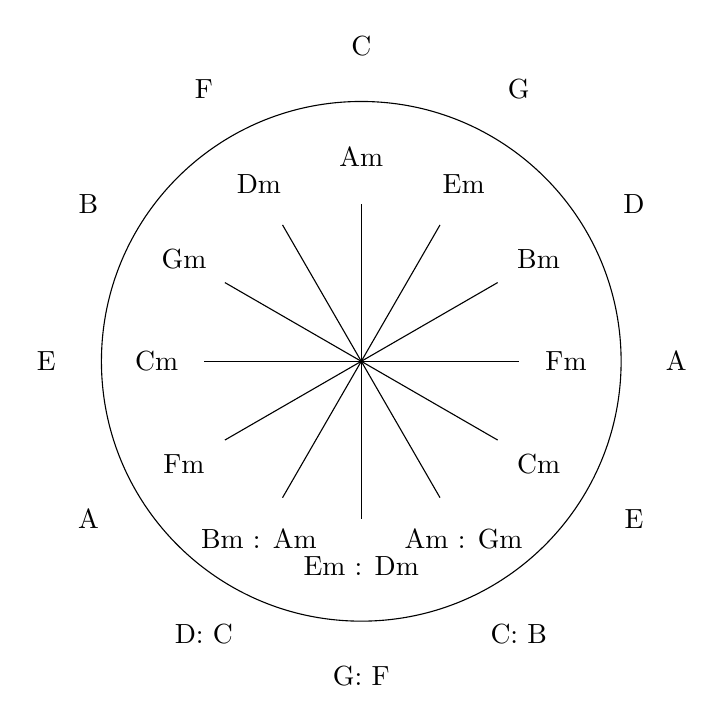
\begin{tikzpicture} % tikzpicture環境開始
\foreach \angle / \label / \Label in
{%
	 90/C/Am, 120/F/Dm, 150/B\aFlat/Gm,
	 180/E\aFlat/Cm, 210/A\aFlat/Fm, 240/D\aFlat : C\aSharp/B\aFlat m : A\aSharp m,
	 270/G\aFlat : F\aSharp/E\aFlat m : D\aSharp m/, 300/C\aFlat : B/A\aFlat m : G\aSharp m/, 330/E/C\aSharp m,
	 0/A/F\aSharp m, 30/D/Bm, 60/G/Em
}
{%
	\draw (\angle:0cm) -- (\angle:2.0cm); 
	\node at (\angle:2.6cm) {\Label};
	\node at (\angle:4.0cm) {\label};
};
\draw (0,0) circle [radius=3.3cm];
\end{tikzpicture} % tikzpicture環境終了
\end{document}

  \caption{五度圏}\figlabel{circle_of_fifths}
\end{center}
\end{figure}

\section{転調の種類}
転調するときに,目的調へ1回の転調のみで到達するものを\KeyBF{直接転調}といい,
目的調までに複数の調を経由して転調するものを\KeyBF{間接転調}といいます.
また間接転調の際に間に挟まれる調を\KeyBF{経過調}といい,
この経過調を速やかに移行する間接転調を\KeyBF{経過転調}といいます.

\section{転調の方法概論}
転調の方法はいくつかの種類分けが可能です.

\begin{description}
\item[直接転調]
出発調のコードから目的調のコードへ直接進行するものです.
シンプルな分,調の関係によっては違和感を生じることがあります.

\item[共通和音を用いた転調]
出発調と目的調での\KeyBF{共通和音}を使い,その機能を転換して転調するものです.
この共通和音のことを\KeyBF{ピボットコード}\xkanjispace(pivot chord,\ common chord)と言います.

\item[ドミナント7thを用いた転調]
基本的には直接転調と同じですが,転調する際に
目的調の\Gnv\subsc{(7)}---\Gni(\Min)という進行をすることでより転調を印象付けるものです.
更にこのドミナント7thコードも\Gnii\Min\subsc7---\Gnv\subsc7に分割したりすることが可能です.
\end{description}

\section{直接転調}
直接転調はポピュラーソングにおいてはサビ前の全音あるいは半音上がる転調のように
使われることが多いものです.
これについて理論的な裏付けをすることはあまり意味を持たないことです.
というのは,この種の転調はそのあからさまな音域上昇を目的としたものが多く,
色彩変化の域にとどまりうるということが理由に挙げられます.

\begin{Yodan}
別に統計を取ったとかではないのですが,このような転調が行われるのはトニックによって終止された直後であったり
ドミナントからそのまま目的調のドミナントへ進むことが多いような気がします.
\end{Yodan}

また時に和音を移高させることで和音進行を作ることがあります.
このとき各和音毎に直接転調していると考えることも出来ます.

%直接転調はその色彩変化の域にとどまる傾向にあることから,調の主音が大きく変化するような場合というのは
%あまり見られないような気がします

\section{共通和音を用いた転調}
共通和音を用いた転調は古典的な楽曲にもよく見られるもので,重要な技法のひとつと言えます.
共通和音を用いた転調は次の三種類に分けることができます
\begin{itemize}
  \item (半音変化を伴わない)調性内和音を共通和音とする近親調または遠隔調への転調
  \item 半音変化を伴う和音を共通和音とする転調
  \item エンハーモニック転換を伴う転調
\end{itemize}

共通和音を用いた転調では多くの場合,共通和音の出発調での機能と目的調での機能を転換する必要があります.
この機能の転換を\KeyBF{転調の作用}と言い,共通和音に目的調の終止形をつけることで達成されます.
\begin{Yodan}%
目的調の終止形をつけることで機能の転換が達成される理由として,T・D・Sの3つの和音を使用することで%
調の構成音がすべて使用されるということが挙げられます.
つまり,終止形をつけることによって完全にその調へ移行したとはっきり示されるのです.
ただし実際にはSが省略され,目的調の属七の和音\Gnv\subsc7が使用されることがあります.
これはDの属七の和音が目的調の上・下属音をもち,一つの調に通常一つしか現れないことから
調を確定することが可能になるためです.
\end{Yodan}
共通和音が目的調でどのような機能を持つかにより,転調の作用がどのように構成されるかが変わります.
\begin{itemize}
  \item 共通和音が目的調でのTまたはその代理
  \item 共通和音が目的調でのSまたはその代理
  \item 共通和音が目的調でのDまたはその代理
\end{itemize}

1番目の場合,共通和音がTまたはその代理ですから,そのあとに目的調での終止形をつける必要があります.
つまり,共通和音と目的調のS,D,Tの3つの和音によって転調が完了します.

2番目の場合,共通和音がSまたはその代理ですから,そのあとに目的調でのD---Tをつなげて終止形を作ればよいです.
つまり,共通和音と目的調のD,Tの3つの和音によって転調が完了します.

3番目の場合,共通和音がDまたはその代理ですから,そのあとに目的調でのTをつなげればよいです.
これは,DからSへとつなげることは通常できないからです.
しかしこの場合Sが終止形に含まれないので不完全なものとなります.
これを解消するために,通常Dの後に目的調の属七の和音\Gnv\subsc7を挟むことが行われます.
この方法による場合,この転調は一種の省略形と見ることができます.
この省略形による転調は速やかに行うことができるので,特に経過転調に好まれます.

\subsection{調性内和音を共通和音とする近親調または遠隔調への転調}
ある長三和音は,複数の調に属しうるということは容易に分かると思います.
例えばCというコードがあったときには次の可能性があります.
\begin{itemize}
  \item C Majの\Gni ,A minの\bFlat\Gniii
  \item G Majの\Gniv ,E minの\bFlat\Gnvi
  \item F Majの\Gnv ,D minの\bFlat\Gnvii
  \item F minの\Gnv
\end{itemize}

この内,G MajおよびE minから見たF MajおよびD min,またその逆は互いに遠隔調の関係になっています.
またF minという調はその他の調と遠隔調の関係になっています.

同様にしてC\Min というコードは
\begin{itemize}
  \item C minの\Gni\Min ,E\aFlat Majの\Gnvi\Min
  \item G minの\Gniv\Min ,B\aFlat Majの\Gnii\Min
  \item F minの\Gnv\Min ,A\aFlat Majの\Gniii\Min
  \item G Majの\Gniv\Min
\end{itemize}
という可能性があります.
ただし\Gnv\Min については上行導音を持たないため,調を確定させる作用に乏しく使用されるのはまれなようです.

C\Dimt というコードは
\begin{itemize}
  \item D\aFlat Majの\Gnvii\Dimt ,B\aFlat minの\Gnii\Dimt
  \item \<(D\aFlat minの\Gnvii\Dimt)
  \item B\aFlat Majの\Gnii\Dimt
\end{itemize}
として\footnote{%
括弧書きしたものについては,通常使われる調ではないという理由がある.
エンハーモニック転換をすればD\aFlat minはC\aSharp minであり,普通に使われる調になるが,それについてはエンハーモニック転換を伴う転調の項で扱う.
},C\Aug というコードは
\begin{itemize}
  \item A minの\Gniii\Aug
  \item E Majの\bFlat\Gnvi\Aug
\end{itemize}
として考えられます.

\begin{Music}[.6\linewidth]
  \nostartrule%
  \generalsignature{0}%
  \Startpiece
  \znotes\lchordsl{C:}\lchordsll{A\Min:}\en%
  \Notes%
  \zchordsl{\Gni}\zchordsll{\bFlat\Gniii}\zw{2}\zw{0}\wh{-2}%
  \en\setdoublebar\generalsignature{1}\ignorenats\changecontext%
  \znotes\lchordsl{G:}\lchordsll{E\Min:}\en%
  \Notes%
  \zchordsl{\Gniv}\zchordsll{\bFlat\Gnvi}\zw{2}\zw{0}\wh{-2}%
  \en\setdoublebar\generalsignature{-1}\ignorenats\changecontext%
  \znotes\lchordsl{F:}\lchordsll{D\Min:}\en%
  \Notes%
  \zchordsl{\Gnv}\zchordsll{\bFlat\Gnvii}\zw{2}\zw{0}\wh{-2}%
  \en\setdoublebar\generalsignature{-4}\ignorenats\changecontext%
  \znotes\lchordsl{F\Min:}\en%
  \Notes%
  \zchordsl{\Gnv}\zw{2}\zw{=0}\wh{-2}%
  \en\setdoublebar%
  \endpiece
  \generalsignature{-3}%
  \Startpiece
  \znotes\lchordsl{C\Min:}\lchordsll{E\aFlat:}\en%
  \Notes%
  \zchordsl{\Gni\Min}\zchordsll{\Gnvi\Min}\zw{2}\zw{0}\wh{-2}%
  \en\setdoublebar\generalsignature{-2}\ignorenats\changecontext%
  \znotes{\lchordsl{G\Min:}}{\lchordsll{B\aFlat:}}\en%
  \Notes%
  \zchordsl{\Gniv\Min}\zchordsll{\Gnii\Min}\zw{2}\zw{0}\wh{-2}%
  \en\setdoublebar\generalsignature{-4}\ignorenats\changecontext%
  \znotes\lchordsl{F\Min:}\lchordsll{A\aFlat:}\en%
  \Notes%
  \zchordsl{\Gnv\Min}\zchordsll{\Gniii\Min}\zw{2}\zw{0}\wh{-2}%
  \en\setdoublebar\generalsignature{1}\ignorenats\changecontext%
  \znotes\lchordsl{G:}\en%
  \Notes%
  \zchordsl{\Gniv\Min}\zw{2}\zw{_0}\wh{-2}%
  \en\setdoublebar%
  \endpiece
  \generalsignature{-5}%
  \Startpiece
  \znotes\lchordsl{D\aFlat:}\lchordsll{B\aFlat\Min:}\en%
  \Notes%
  \zchordsl{\Gnvii\Dimt}\zchordsll{\Gnii\Dimt}\zw{2}\zw{0}\wh{-2}%
  \en\setdoublebar\generalsignature{-2}\ignorenats\changecontext%
  \znotes\lchordsl{B\aFlat:}\en%
  \Notes%
  \zchordsl{\Gnii\Dimt}\zw{_2}\zw{0}\wh{-2}%
  \en\setdoublebar%
  \endpiece%
  \generalsignature{0}%
  \Startpiece%
  \znotes\lchordsl{A\Min:}\en%
  \Notes%
  \zchordsl{\bFlat\Gniii\Aug}\zw{^2}\zw{0}\wh{-2}%
  \en\setdoublebar\generalsignature{4}\ignorenats\changecontext%
  \znotes\lchordsl{E:}\en%
  \Notes%
  \zchordsl{\bFlat\Gnvi\Aug}\zw{2}\zw{0}\wh{=-2}%
  \en\setdoublebar%
  \endpiece
\end{Music}

これらを共通和音として転調に用いることができます.


\subsection{半音変化を伴う和音を共通和音とする転調}
半音変化を伴う和音を頻繁に使うと,時に調性が不安定になることがあります.
これはこの種の和音が時に他調の雰囲気を表すからであると言えます.
通常このように導入された他調の雰囲気は原調の終止形によって取り払われるものですが,
原調ではなくその新しい調に終止することで転調を行うことが可能になります.
この種の転調を\KeyBF{半音階的転調}とか,\KeyBF{クロマチック転調}と呼びます

これは出発調においてノンダイアトニック・コードで目的調において調性内和音という形でもよいですし,
その逆,またはどちらの調においてもノンダイアトニック・コードであるということも可能です.
\begin{Music}
  \generalmeter{\meterC}%
  \generalsignature{0}%
  \setstaffs{1}{2}\setclef{1}{6}%
  \Startpiece
  \NOTes%
  \ha{3}%
  \ha{6}%
  |\zchordsu{C}\zh{5}\zh{2}\hu{0}%
  \zchordsu{F}\zh{5}\zh{3}\hu{1}%
  \en\bar%
  \NOTes%
  \ha{7}%
  \ha{5}%
  |\zchordsu{G}\zh{4}\zh{2}\hu{-1}%
  \zchordsu{C/E}\zh{5}\zh{2}\hu{-2}%
  \en\bar%
  \NOTes%
  \zchordsl{\Gnii\Min}\ha{4}%
  \lrchordsl{es:&\Gniv\Min\subsc6}\ha{_8}%
  |\zchordsu{D\Min}\zh{6}\zh{3}\hu{1}%
  \zchordsu{A\aFlat\Min\subsc6}\zh{_7}\fl[l]{5}\zh{5}\hl{1}%
  \en\bar%
  \NOTes%
  \ha{_9}%
  \ha{_2}%
  |\zchordsu{\hspace{-\QNwidth}E\aFlat\Min/B\aFlat}\zh{_7}\fl[l]{4}\zh{4}\hl{_2}%
  \zchordsu{B\aFlat}\zh{6}\zh{4}\hu{1}%
  \en\bar%
  \NOTEs%
  \wh{_5}%
  |\zchordsu{E\aFlat\Min}\zw{_7}\fl[l]{4}\zw{4}\wh{_2}%
  \en\setdoublebar%
  \endpiece
\end{Music}


\subsection{エンハーモニック転換を伴う転調}\ssectlabel{enharmonic_modulation}
エンハーモニック転換を伴う転調とは,共通和音の構成音の全てあるいは一部に対してエンハーモニック転換を行うものです.
\subsubsection{全ての構成音にエンハーモニック転換を行う例}
全ての構成音にエンハーモニック転換を行う例は少ないと言えます.
先に上げたD\aFlat Maj調でのC\Dimt とC\aSharp min調でのB\aSharp\Dimt は1つの例といえます.

\begin{Music}[.6\linewidth]
  \nostartrule%
  \generalsignature{-5}%
  \Startpiece
  \Notes%
  \lrchordsl{Des:&\Gnvii\Dimt}\zchordsu{C\Dimt}\zw{2}\zw{0}\wh{-2}%
  \en\setdoublebar\generalsignature{+4}\ignorenats\changecontext%
  \Notes%
  \lrchordsl{cis:\hspace{\QNwidth}&\Gnvii\Dimt}\zchordsu{B\aSharp\Dimt}\zw{1}\zw{-1}\wh{^-3}%
  \en\setdoublebar
  \endpiece
\end{Music}


\subsubsection{一部の構成音にエンハーモニック転換を行う例}
一部の構成音にエンハーモニック転換を行う和音の特に重要な例として,減七の和音や増三和音,増三四六の和音
(あるいはエンハーモニック転換して\txCirc\lhsc{7}{\bFlat5})があげられます.
これらは隣り合う構成音間の音程に対称性があります.
例えば減七の和音は半音3つ分の間隔で,増三和音は半音4つ分の間隔で各構成音が存在しています.
また増三四六の和音は半音4つ分と半音2つ分の繰り返しとなっています.
この対称性は容易に響きを保ったまま転義することを可能にします.

\begin{Music}[.7\linewidth]
  \nostartrule%
  \Startpiece
  \Notes%
  \zchordsu{G\aSharp\Dim\subsc7}\zw{1}\zw{-1}\zw{-3}\wh{^-5}%
  \en%
  \Notes\zchordsu{$=$}\en%
  \Notes%
  \zchordsu{B\Dim\subsc7}\zw{_3}\zw{1}\zw{-1}\wh{-3}%
  \en%
  \Notes\zchordsu{$=$}\en%
  \Notes%
  \zchordsu{D\Dim\subsc7}\zw{_5}\fl[l]{3}\zw{3}\zw{1}\wh{-1}%
  \en%
  \Notes\zchordsu{$=$}\en%
  \Notes%
  \zchordsu{F\Dim\subsc7}\zw{_7}\fl[qll]{5}\zw{5}\fl[ql]{3}\zw{3}\zw{1}%
  \en%
  \Notes\zchordsu{$=$}\en%
  \Notes%
  \zchordsu{A\aFlat\Dim\subsc7$=$G\aSharp\Dim\subsc7}\zw{<9}\fl[ll]{7}\zw{7}\fl[ql]{5}\zw{5}\fl[qll]{3}\zw{3}%
  \en%
  \endpiece
  \Startpiece
  \Notes%
  \zchordsu{A\aFlat\Aug}\zw{0}\zw{-2}\wh{_-4}%
  \en%
  \Notes\zchordsu{$=$}\en%
  \Notes%
  \zchordsu{C\Aug}\zw{^2}\zw{0}\wh{-2}%
  \en%
  \Notes\zchordsu{$=$}\en%
  \Notes%
  \zchordsu{E\Aug}\zw{^4}\sh[l]{2}\zw{2}\wh{0}%
  \en%
  \Notes\zchordsu{$=$}\en%
  \Notes%
  \zchordsu{G\aSharp\Aug$=$A\aFlat\Aug}\zw{>6}\sh[hll]{4}\zw{4}\sh[hl]{2}\wh{2}%
  \en%
  \endpiece
  \generalsignature{0}%
  \Startpiece
  \Notes%
  \zchordsu{F\lhsc{7}{\bFlat5}}\zw{_7}\fl[l]{5}\zw{5}\zw{3}\wh{1}%
  \en%
  \Notes\zchordsu{$=$}\en%
  \Notes%
  \zchordsu{C\aFlat\lhsc{7}{\bFlat5}}\dfl{11}\dfl[hll]{9}\fl[ql]{7}\fl[l]{5}\zw{11}\zw{9}\zw{7}\wh{5}%
  \en%
  \Notes\zchordsu{$=$}\en%
  \Notes%
  \zchordsu{B\lhsc{7}{\bFlat5}}\zw{10}\zw{8}\zw{^6}\wh{4}%
  \en%
  \endpiece
\end{Music}



\section{ドミナント7thを用いた転調}
ドミナント7thを用いた転調は直接転調の発展版と言えるもので,多少無理のある調へ進んでも
違和感を少なくすることができます.
これはまた,半音変化を伴う和音を共通和音とする転調と言えなくもないですが,
そのように解釈するよりもこちらのほうが実践的であると考えることができます.
\begin{Music}
  \interstaff{14}%default:9
  \generalmeter{\meterC}%
  \generalsignature{0}%
  \setstaffs{1}{2}%
  \setclef{1}{\bass}%
  \Startpiece
  \NOtes
  \zql{3}\qu{12}%
  \figbassuuu[6]\zql{5}\qu{10}%
% \figbassuuu[3][\txSharp4][6]\lchordsl{a:\ }\zchordsl{\Gnvii\subsc7}\zql{4}\qu{9}%
  \figbassuuu[3][\txSharp4][6]\lrchordsl{A:&\Funktion{\Stellung{\Slash D}{7}\Hochgestellt{9\tiefalt}}}\zql{4}\qu{9}%
% \figbassuuu[6]\zchordsl{\Gni\subsc\txSharp}\zql{^3}\qu{8}%
  \figbassuuu[6]\zchordsl{\Funktion{\Stellung{T}{3}}}\zql{^3}\qu{8}%
  |\zql{2}\qu{5}%
  \zql{0}\qu{2}%
  \rql{1}\qu{^2}%
  \zql{0}\qu{3}%
  \en\bar
  \NOtes
% \figbassuuu[\txSharp][7]\lchordsl{H:\ }\zchordsl{\Gnv\subsc7}\zql{^6}\qu{10}%
  \figbassuuu[\txSharp][7]\lrchordsl{H: &\Funktion{D\Hochgestellt{\subsupsc{5\tiefalt}7}}}\zql{^6}\qu{10}%
% \figbassuuu[\txSharp][6]\zchordsl{\Gni}\zql{^4}\qu{9}%
  \figbassuuu[\txSharp][6]\cchordsl{\Funktion{\Stellung{T}{3}}}\zql{^4}\qu{9}%
% \figbassuuu[\txFlat5][\txSharp6]\lchordsl{g:\ }\zchordsl{\Gniv\subsupsc*{5}{\btxSharp6}}\fl[ql]{5}\zql{5}\qu{_9}%
  \figbassuuu[\txFlat5][\txSharp6]%
    \lrchordsl{G:&\Funktion{\Stellung{\Slash{\WechselD}}{5\tiefalt}\Hochgestellt{\subsupsc7{9\tiefalt}}}}%
    \fl[ql]{5}\zql{5}\qu{_9}%
% \figbassuuu[\txSharp]\lchordsll{G:\ }\zchordsll{\Gnv}\zchordsl{\Gnv}\zql{=4}\qu{8}%
  \figbassuuu[\txSharp]\zchordsl{\Funktion{D}}\zql{=4}\qu{8}%
  |\zql{0}\qu{^3}%
  \zql{^1}\qu{4}%
  \zql{2}\qu{^5}%
  \zql{1}\qu{6}%
  \en\bar%\hardspace{\QNwidth}%
  \NOtes
% \figbassuuu[6]\zchordsll{\Gnvi}\zql{7}\parna{9}\qu{9}%
  \figbassuuu[6]\zchordsl{\Funktion{\Stellung{Tp}{3}}}\zql{7}\parna{9}\qu{9}%
  \figbassuuuu[3][4][\txSharp6]\zql{8}\qu{^11}%
  \figbassuuuu[6]\zql{7}\qu{12}%
% \figbassuuuu[\txFlat][5][6]\lchordsl{C:\ }\zchordsl{\Gnii\subsupsc56}\zql{6}\qu{=11}%
  \figbassuuuu[\txFlat][5][6]\lrchordsl{C: &\Funktion{s\Hochgestellt{\subsupsc56}}}\zql{6}\qu{=11}%
  |\zql{2}\qu{7}%
  \zql{5}\qu{^8}%
  \zql{4}\qu{9}%
  \zql{5}\qu{_10}%
  \en\bar%
  \NOtes
% \figbassuuuu[4][6]\zchordsl{\Gni\subsupsc46}\zhl{7}\hu{12}%
  \figbassuuuu[4][6]\zchordsl{\Funktion{D\Hochgestellt{\subsupsc46}}}\zhl{7}\hu{12}%
  \figbassuuuu[---][---]\sk%
  \figbassuuuu[3][5]\zhl{0}\hu{9}%
  \figbassuuuu[7]\sk%
  |\zql{5}\qu{9}%
  \zql{2}\qu{5}%
  \zql{2}\hu{6}%
  \ql{1}%
  \en\bar%
  \NOTes
  \zw{3}\wh{10}%
  |\zw{0}\wh{5}%
  \en\setdoublebar%
  \endpiece%
\end{Music}
%\begin{chuui}
%下に示したローマ数字による和声記号はその骨格を示すもので,正確な形を示しているものではないことに注意.
%\end{chuui}

ドミナント7thによって転調した先で,さらにドミナント7thを用いて連続で転調することが可能です.
次は最も極端な例と言えるでしょう.

\begin{Music}
  \generalmeter{\meterC}%
  \generalsignature{0}%
  \setstaffs{1}{2}\setclef{1}{\bass}%
  \Startpiece
  \NOTes%
  \ha{9}|\zchordsu{B\subsc7}\zh{^6}\zh{3}\sh[ql]{1}\hu{1}%
  \en%
  \NOTes%
  \ha{5}|\zchordsu{E\subsc7}\zh{=6}\sh[ql]{2}\zh{2}\hu{0}%
  \en\bar%
  \NOTes%
  \ha{8}|\zchordsu{A\subsc7}\zh{^5}\zh{2}\hu{0}%
  \en%
  \NOTes%
  \ha{4}|\zchordsu{D\subsc7}\zh{=5}\sh[ql]{1}\zh{1}\hu{-1}%
  \en\bar%
  \NOTes%
  \ha{7}|\zchordsu{G\subsc7}\zh{4}\zh{1}\hu{-1}%
  \en%
  \NOTes%
  \ha{3}|\zchordsu{C\subsc7}\zh{_4}\zh{0}\hu{-2}%
  \en\bar%
  \NOTes%
  \ha{6}|\zchordsu{F\subsc7}\zh{3}\zh{_0}\hu{-2}%
  \en%
  \NOTes%
  \ha{_2}|\zchordsu{B\aFlat\subsc7}\zh{_3}\zh{-1}\hu{_-3}%
  \en\bar\addspace{.2\afterruleskip}%
  \NOTes%
  \ha{_5}|\zchordsu{E\aFlat\subsc7}\zh{2}\zh{_-1}\fl[hl]{-3}\hu{-3}%
  \en%
  \NOTes%
  \ha{_1}|\zchordsu{A\aFlat\subsc7}\zh{_2}\zh{-2}\hu{_-4}%
  \en\bar%
  \NOTes%
  \ha{_4}|\zchordsu{D\aFlat\subsc7}\zh{1}\zh{_-2}\fl[hl]{-4}\hu{-4}%
  \en%
  \NOTes%
  \ha{_0}|\zchordsu{G\aFlat\subsc7}\zh{_1}\fl[ql]{-3}\zh{-3}\fl[qhl]{-5}\hu{-5}%
  \en\bar%
  \notes\sk\en%
  \NOTEs%
  \wh{_3}|\zchordsu{C\aFlat\subsc7($=$B\subsc7)}\zw{_0}\dfl[qhl]{-3}\zw{-3}\wh{_-5}%
  \en\setdoublebar%
  \endpiece
\end{Music}

この場合,各和音で次の和音の根音を主音とする調に転調していると考えられます.


\chapter{非機能的なハーモナイズ・リハーモナイズ}
機能和声から外れた和音進行も,ある程度の理由付けが可能であれば実用に耐えうるものになります.
\sectref{AlteredFifth}や\sectref{ChPassing},\sectref{DimPassing}などもその一例です.
この種の和声は機能の効力が弱められ,また混合しているために曖昧な変化を感じさせます.

\section{偶成和音の活用}
機能的に良くないとされる\Funktion{D}---\Funktion{S}の接続であっても,どちらか(あるいはどちらも)が偶成和音として解釈されるような場合は
悪作用は取り除かれます.
それ以外であっても偶成和音と解釈される場合には,その和音は装飾的なものと解釈されます.

\begin{Music}
  \setstaffs{1}{2}%
  \setclef{1}{\bass}%
  \interstaff{10}%default:9
%  \setname{1}{\piecenum}
%  \nostartrule%
%  \generalsignature{1}%
  \generalmeter{\meterfrac{3}{4}}%
  \Startpiece%
  \NOtes
  \zchordsl{T}\ha{3}%
  \lrchordsl{|&S|}\sk%
  \zchordsl{T}\qa{3}%
  |\zq{0}\zq{-2}\qu{-5}%
  \zq{1}\zq{-2}\qu{-4}%
  \zq{2}\zq{0}\qu{-2}%
  \en\bar
  \NOtes
  \zchordsl{D}\qa{2}%
  \lrchordsl{|&S|}\qa{1}%
  \zchordsl{D\subsc7}\qa{0}%
  |\zq{2}\rq{-1}\qu{-1}%
  \zq{3}\zq{1}\qu{-2}%
  \zq{4}\zq{1}\qu{-1}%
  \en\bar
  \NOtes
  \zchordsl{T}\qa{-2}%
  \zchordsl{S}\qa{-1}%
  \zchordsl{D}\qa{0}%
  |\zq{5}\zq{2}\qu{-2}%
  \zq{3}\zq{1}\qu{-2}%
  \zq{2}\zq{-1}\qu{-3}%
  \en\bar
  \NOtes
  \lrchordsl{|&S|}\ha{3}%
  \sk
  \zchordsl{T}\qa{3}%
  |\zq{1}\zq{-2}\qu{-4}%
  \zq{-1}\zq{-4}\qu{-6}%
  \zq{0}\zq{-2}\qu{-5}%
  \en\setdoublebar
  \endpiece%
\end{Music}
%偶成和音として解釈されるようなものというのは次のようなものです.
%\begin{description}
%  \item[経過和音]
%  \item[刺繍和音]
%  \item[倚和音]
%  \item[オルガンポイント]
%\end{description}

\section{同種和音による和声付け(constant structure)}
メロディに対して一定の構造を持った和音をつけることで,一つの旋律を和音によって
重層化したものというように聴くことができるようになります.
このような手法を\eghostguarded{\KeyBF{constant structure}}といいます.
この手法は,通常の和声法のように反行や斜行を組み合わせたような進行をさせれば
たちまち声部の区別がつかなくなるであろうような複雑な和音に対して用いられることが多いですが,
そうではない簡素な和音に対しても用いることが可能です.

\begin{Music}
%  \setstaffs{1}{2}%
%  \setclef{1}{\bass}%
%  \interstaff{10}%default:9
%  \setname{1}{\piecenum}
  \nostartrule%
%  \generalsignature{1}%
  \generalmeter{\meterC}%
  \Startpiece%
  \NOtes\zchordsu{(C\supsc{(9)}\Sus4)}%
  \zq{5}\rq{2}\zq{1}\qu{-1}%
  \zq{6}\rq{3}\zq{2}\qu{0}%
  \zq{7}\rq{4}\zq{3}\qu{^1}%
  \zq{8}\zq{5}\lq{_4}\ql{2}%
  \en\bar
  \NOtes
  \zq{7}\rq{4}\zq{3}\qu{^1}%
  \zq{6}\rq{3}\zq{2}\qu{0}%
  \en\NOTes
  \zh{5}\rh{2}\zh{=1}\hu{-1}%
  \en\doublebar
  \NOtes\zchordsu{(A\subsc7\supsc{\bSharp9})}%
  \zq{5}\rq{3}\zq{2}\qu{^-2}%
  \zq{6}\rq{4}\zq{3}\qu{^-1}%
  \zq{7}\sh[l]{5}\zq{5}\lq{4}\ql{^0}%
  \zq{8}\zq{6}\lq{=5}\ql{^1}%
  \en\bar
  \NOtes
  \zq{7}\sh[l]{5}\zq{5}\lq{4}\ql{^0}%
  \zq{6}\lq{4}\zq{3}\qu{^-1}%
  \en\NOTes
  \zh{5}\rh{3}\zh{2}\hu{^-2}%
  \en\setdoublebar
  \endpiece%
  \piececaption{add 9th sus4コードおよび7(\bSharp9)コードによるハーモナイズをした\\「かえるの合唱」.}%
\end{Music}

\begin{Music}
  \setstaffs{1}{2}%
  \setclef{1}{\bass}%
%  \interstaff{10}%default:9
%  \setname{1}{\piecenum}
%  \generalsignature{1}%
  \generalmeter{\meterC}%
  \Startpiece%
  \NOTEs
  \wh{c}%
  |\zchordsu{C}\zw{'e}\zw{'g}\wh{''c}%
  \en\bar
  \NOTEs
  \fl{e}\wh{e}%
  |\zchordsu{E\aFlat}\fl{''e}\fl[l]{'b}\zw{'g}\zw{'b}\wh{''e}%
  \en\bar
  \NOTEs
  \wh{f}%
  |\zchordsu{F}\zw{'a}\zw{''c}\wh{''f}%
  \en\bar
  \NOTEs
  \wh{g}%
  |\zchordsu{G}\zw{'b}\zw{''d}\wh{''g}%
  \en\setdoublebar
  \endpiece\vspace{-.5\baselineskip}%
  \piececaption{この種のコード進行はバスによるマイナー・ペンタトニック・スケールの\\メロディを長三和音でハーモナイズしたものとしても考えられる.}%
\end{Music}

次に示すのはMaurice Ravelの``Pavane pour une infante défunte''の25小節目からの抜粋です.
26小節の3拍目から27小節2拍目までにかけて,同じ構造(\txSqr\subsc9)の和音が並進行しながら使用されているのが分かります.

\begin{Music}
  \settowidth{\parindent}{Pf.}%
  \setstaffs{1}{2}%
  \setclef{1}{\bass}%
  \interstaff{15}%default:9
  \setname{1}{Pf.}%
%  \nostartrule%
  \generalsignature{1}%
  \generalmeter{\meterC}%
  \Startpiece%
  \Notes
  \Mryaku\sk|\Mryaku\sk\islurd0{-5}\isluru1{8}%
  \en\barnumbers\barno24\def\freqbarno{24}\bar\addspace{.3\afterruleskip}%
  \NOtes
  \zq{2}\qu{-2}%
  |\zchordsuu{E\lhsc9{13}}\lst{-5}\tslur0{-5}\zq{1}\rq{-1}\zq{^-2}\sh[hql]{-5}\qu{-5}%
  \en\NOtesp
  \zmidstaff{\mp}\zqp{5}\qup{1}%
  |\zchordsuu{A\subsc9}\lst{-5}\tbsluru1{2}\roff{\pt{1}\pt{-1}\pt{-3}\pt{-5}}\zq{0}\rq{-2}\zq{-3}\na{-5}\qu{-5}%
  \en\Notes
  \Ibu0{8}{2}2\zqb0{8}\qb0{4}\zqb0{5}\qb0{1}\zqb0{2}\tqu0{-2}%
  |\zchordsuu{D\subsc6}\Ibu0{1}{3}2\islurd0{-7}\lst{-6}\zqb0{-1}\zqb0{-3}\qb0{-6}%
  \zchordsuu{A\subsc9}\lst{-5}\zqb0{0}\rqb0{-2}\zqb0{-3}\qb0{-5}%
  \zchordsuu{E\lhsc9{13}}\lst{-5}\zqb0{1}\rqb0{-1}\zqb0{-2}\tqu0{^-5}%
  \en\bar\addspace{.3\afterruleskip}%
  \NOtes
  \icresc\ibsluru2{5}\zq{5}\qu{1}%
  |\zchordsuu{A\subsc9}\flatslur\islurd8{-5}\zq{0}\sh{-2}\rq{-2}\zq{-3}\loffset{2}{\lpar{-5}\rpar{-5}}\na[hql]{-5}\qu{-5}%
  \en\Notes
  \zmidstaff{\tdecresc}\tslur2{8}\zq{8}\cl{4}%
  \ds
  |\zchordsuu{D}\tslur8{-6}\tslur0{-6}\zq{-1}\zq{-4}\cu{-6}%
  \ds
  \en\NOtes
  \lsf{-2}\zq{2}\qu{-2}\zmidstaff{\f}\itied8{-3}\itieu1{1}\lsf{-3}\zq{1}\qu{-3}%
  |\zchordsuu{E\subsc9}\roff{\highslur\isluru0{8}}\usf{6}\zq{1}\zq{-1}\qu{^-5}%
  \zchordsuu{D\subsc9}\usf{6}\itied2{-6}\itieu3{-2}\itieu4{0}\zq{0}\zq{=-2}\qu{-6}%
  \en\bar
  \Notes
  \ttie8\ttie1\ibu0{1}0\zqb0{1}\qb0{-3}%
  \lsf{-4}\zqb0{0}\qb0{-4}%
  \lsf{-3}\zqb0{1}\qb0{-3}%
  \lsf{-2}\zqb0{2}\tqu0{-2}%
  |\ttie2\ttie3\ttie4\ibu0{0}0\zqb0{0}\zqb0{-2}\qb0{-6}%
  \zchordsuu{C\subsc9}\busf0\zqb0{-1}\zqb0{_-3}\qb0{-7}%
  \zchordsuu{D\subsc9}\busf0\zqb0{0}\zqb0{-2}\qb0{-6}%
  \zchordsuu{E\subsc9}\busf0\zqb0{1}\zqb0{-1}\tqu0{^-5}%
  \en\addspace{1.5\QNwidth}\Notes
  \islurd1{0}\zchar{-8}{\decrescendo{2\noteskip}}\zq{4}\qu{0}%
  |\zchordsuu{Gm\lhsc7{13}}\zchar{10}{\decrescendo{2\noteskip}}\ibsluru2{0}\highslur\ibslurd3{-6}%
  \ibl0{-6}0\na[l]{-5}\na[lhql]{-6}\zq{0}\zqu{-3}\lqb0{-6}\qb0{-5}%
  \en\addspace{2\QNwidth}\Notes
  \sk
  |\loff{\itied8{-6}}\sh[l]{-5}\sh[ll]{-6}\lqb0{-6}\tql0{-5}%
  \en\NOtes
  \tslur1{-3}\fermataup{8}\zq{1}\qu{-3}%
  |\zchordsuu{D\subsc7}\fermataup{8}\tslur0{8}\tslur2{4}\tslur3{-6}\ttie8\rq{-1}\zq{-2}\zq{-4}\qu{-6}%
  \en\setdoublebar
  \endpiece%
  \piececaption{Pavane pour une infante défunte (Maurice Ravel)}%
\end{Music}

この手法は複数の旋律に対して適用されることも可能です.
その場合にはより複雑な響きが得られるでしょう.


\section{ダイアトニック・コードによる和声付け}
ダイアトニック・コード同士の接続はどのように選んでも(比較的)破綻しづらいという特徴があるため,
非機能的な接続を選んでも調性を保つことが可能といえます.

\begin{Music}[.6\linewidth]
  \setstaffs{1}{2}%
  \setclef{1}{\bass}%
  \interstaff{10}%default:9
%  \setname{1}{\piecenum}
%  \nostartrule%
%  \generalsignature{1}%
%  \generalmeter{\meterfrac{2}{4}}%
  \Startpiece%
  \NOTes
  \ha{3}|\zchordsu{C}\zh{5}\zh{2}\hu{0}%
  \en\NOtesp
  \qap{4}|\zchordsu{Dm}\zqp{3}\zqp{1}\qup{-1}%
  \en\Notes
  \itied0{5}\ca{5}|\zchordsu{Em}\itieu1{2}\zq{2}\itied2{0}\zq{0}\itied3{-3}\cu{-3}%
  \en\bar
  \NOTes
  \ttie0\ha{5}|\ttie1\ttie2\ttie3\zh{2}\zh{0}\hu{-3}%
  \en\NOtes
  \qa{5}\qa{4}
  |\zq{4}\zq{2}\qu{0}%
  \zchordsu{Dm}\zq{6}\zq{3}\qu{1}%
  \en
  \setdoublebar\endpiece%
\end{Music}

全音階的なメロディの場合,その1音1音に対してダイアトニック・コードで和音をつけることによって
リハーモナイズを行うことがあります.

この手法はまた拡張して三度堆積以外のダイアトニック・スケール上に構成される和音を素材に使うことができます.
このような,三度堆積和音に限らない全音階的な和音による和声を
しばしば\KeyBF{汎全音階法}(\KeyBF[汎全音階法]{pandiatonicism})といいます.

\begin{Music}[.6\linewidth]
  \setstaffs{1}{2}%
  \setclef{1}{\bass}%
  \interstaff{10}%default:9
%  \setname{1}{\piecenum}
%  \nostartrule%
%  \generalsignature{1}%
%  \generalmeter{\meterfrac{2}{4}}%
  \Startpiece%
  \znotes\loffset{2}{\islurd0{g}\tinynotesize\grcu{g}}\en\NOtes
  \tslur0{c}\qap{c}%
  |\zq{''c}\rq{'a}\zq{'g}\qu{'d}%
  \en\Notes
  \sk\itieu0{'c}\ca{'c}%
  |\zq{''d}\rq{'b}\zq{'a}\qu{'e}%
  \en\NOtes
  \ttie0\ha{'c}%
  |\zq{''e}\zq{''c}\lq{'b}\ql{'f}%
  \zq{''f}\zq{''d}\lq{''c}\ql{'g}%
  \en\bar
  \NOtes
  |\zq{''e}\zq{''c}\lq{'b}\ql{'f}%
  \zq{''d}\rq{'b}\zq{'a}\qu{'e}%
  \en\NOTes
  |\zh{''c}\rh{'a}\zh{'g}\hu{'d}%
  \en\def\atnextbar{\znotes\centerbar{\duevolte}\en}%
  \setdoublebar\endpiece%
  \piececaption{汎全音階法によるハーモナイズをされた「かえるの合唱」.}%
\end{Music}

\section{共通音を維持した半音階的和音による和声付け}
共通音を多く持つ和音同士の連結は,機能的な和音連結とは異なった印象を与えます.
例えば
\begin{Music}
  \nobarnumbers%
  \nostartrule%
  \Startpiece%
  \Notes%
  \zchordsu{Dm\subsc7}\MlineC{3}[-\WNwidth]{0}\MlineC{1}[-\WNwidth]{0}\zw{5}\zw{3}\zw{1}\wh{-1}%
  \zchordsu{D\aFlat\Aug\subsc7}\MlineC{5}[-\WNwidth]{-1}\zw{_5}\zw{3}\zw{1}\wh{_-1}%
  \zchordsu{G\aSharp\hDim\subsc7}\roff{\MlineC{4}[-2\WNwidth]{0}\MlineC{2}[-2\WNwidth]{0}}\sh{2}\lsh{1}\llna{-1}\zw{4}\rw{2}\zw{1}\wh{-1}%
  \zchordsu{E\subsc{\Maj7}}\roff{\MlineC{0}[-2\WNwidth]{0}}\sh{2}\lsh{-1}\zw{4}\zw{2}\rw{0}\wh{-1}%
  \zchordsu{C\aSharp\Dim\subsc7}\MlineC{4}[-1.1\WNwidth]{0}\MlineC{-2}[-\WNwidth]{1}\fl{4}\na[l]{2}\sh{-2}\zw{4}\zw{2}\zw{0}\wh{-2}%
  \zchordsu{E\aFlat m\subsc7}\roff{\MlineC{-1}[-2\QNwidth]{0}}\fl{4}\lfl{2}\llfl{0}\fl{-1}\zw{4}\zw{2}\rw{0}\wh{-1}%
  \zchordsu{D\aFlat\lhsc{7}{\Minus5}}\MlineC{3}{-1}\fl{5}\ldfl{3}\fl{-1}\zw{5}\zw{3}\zw{1}\wh{-1}%
  \zchordsu{C}\zw{=5}\zw{2}\zw{0}\wh{-2}%
  \en\doublebar
  \Notes%
  \Mryaku\sk
  \zchordsu{G\lhsc{7}{\Minus5}}\roff{\MlineC{2}[-\WNwidth]{0}}\na{4}\lna{2}\loffset{.1}{\fl{-1}}\zw{4}\rw{2}\zw{1}\wh{-1}%
  \zchordsu{C}\zw{=5}\zw{2}\zw{0}\wh{-2}%
  \en\setdoublebar
  \endpiece%
\end{Music}
あるいは;
\begin{Music}
  \nobarnumbers%
  \nostartrule%
  \Startpiece%
  \Notes\lcharsl{common tone}%
  \ibktu[\textit{bis.}]0{16}\zchordsu{E\subsc7\Sus4}\MlineC{6}{0}\MlineC{3}{0}%
  \Mhshift{.5}{\ccharsl{d,a}}%
    \zw{6}\rw{4}\zw{3}\wh{0}%
  \zchordsu{E\aFlat\lhsc{\Maj7}{\Plus11}}\MlineC{6}{0}\Roff{\MlineC{3}[-\WNwidth]{0}}\MlineC{2}{0}%
  \Mhshift{.5}{\ccharsl{d,g,a}}%
    \fl{0}\zw{6}\rw{3}\zw{2}\wh{0}%
  \loff{\tbkt0{16}}\zchordsu{D\subsc7\Sus4}\Roff{\MlineC{5}[-\WNwidth]{0}\MlineC{2}[-\WNwidth]{0}}%
  \Mhshift{.5}{\ccharsl{c,g}}%
    \rw{6}\zw{5}\rw{3}\zw{2}\wh{-1}%
  \zchordsu{D\aFlat\lhsc{\Maj7}{\Plus11}}\MlineC{-1}[-\WNwidth]{-1}%
  \Mhshift{.5}{\ccharsl{des$=$cis}}%
    \fl{-1}\zw{5}\rw{2}\zw{1}\wh{-1}%
  \zchordsu{C\aSharp\subsc7\Sus4}\MlineC{4}{0}\MlineC{1}[-\WNwidth]{0}%
  \Mhshift{.5}{\ccharsl{fis,h}}%
    \sh{2}\sh[l]{1}\sh[ql]{-2}\zw{4}\rw{2}\zw{1}\wh{-2}%
  \zchordsu{C\lhsc{\Maj7}{\Plus11}}\MlineC{7}{0}\MlineC{4}{0}%
  \Mhshift{.5}{\ccharsl{e,h}}%
    \sh{1}\na[l]{-2}\zw{7}\zw{4}\rw{1}\zw{0}\wh{-2}%
  \zchordsu{F\lhsc{\Maj7}{\Plus11}}\MlineC{7}{0}\Roff{\MlineC{4}[-\WNwidth]{0}}\MlineC{3}{0}%
  \Mhshift{.5}{\ccharsl{e,a,h}}%
    \na{1}\zw{7}\rw{4}\zw{3}\wh{1}%
  \zchordsu{E\subsc7\Sus4}%
    \rw{7}\zw{6}\rw{4}\zw{3}\wh{0}%
  \en\setdoublebar
  \endpiece%
  \piececaption{拙作「Yoru-No-Oto」のAメロからBメロ終わりにかけてのコード進行.}%
\end{Music}
%この種の和声は浮遊和声(Roving Harmony)とも呼ばれます.

\section{上部和音構造と独立した低音をもつ和声付け}
上部で機能的・非機能的に進行するコード進行を持ちながら,メロディラインと
反進行するように動く低音を持つ和音連結が使われることがあります.
これを\eghostguarded{\KeyBF{contrary motion}}といいます.
また,これをより一般化して,上部の進行とは独立に上行・下行する低音の線が作られることがあります.

\begin{Music}
  \nobarnumbers%
  \setstaffs{1}{2}%
  \setclef{1}{\bass}%
  \generalsignature{-3}%
  %\interstaff{11}%default:8
  \Startpiece%
  \NOtes
  \qp|\qa{-3}%
  \en\bar
  \NOtes
  \itieu0{9}\itieu1{7}\itied2{5}\zw{9}\zw{7}\wh{5}%
  |\zchordsu{E\aFlat\subsc{\Maj7}}\qa{-2}\qa{-1}\qa{0}\qa{1}%
  \en\bar
  \NOtes
  \midslur{2}\ttie0\midslur{2}\ttie1\midslur{-2}\ttie2\zw{9}\zw{7}\wh{5}%
  |\qa{2}\qa{4}\qa{1}\qa{0}%
  \en\bar
  \NOTEs
  \zw{10}\zw{6}\wh{4}%
  |\zchordsu{D\hDim\subsc7}\itied0{1}\wh{1}%
  \en\bar
  \NOTesp
  \zw{=9}\rw{7}\wh{6}%
  |\zchordsu{G\subsc7}\ttie0\hap{1}%
  \en\NOtes
  |\Mryaku\sk
  \en\setdoublebar
  \endpiece
  \nobarnumbers%
  \setstaffs{1}{2}%
  \setclef{1}{\bass}%
  \generalsignature{-3}%
  \Startpiece
  \NOtes
  \qp|\qa{4}%
  \en\bar
  \NOtes
  \qa{5}\qa{4}\qa{_4}\qa{3}%
  |\zchordsu{E\aFlat\subsupsc{\Maj7}{13}}\zq{5}\zq{2}\qu{-1}%
  \lrchordscuu{(&D\Dimt}\zq{6}\zq{3}\qu{1}%
  \zchordscuu{E\aFlat\Min}\zq{7}\zq{4}\qu{_2}%
  \zchordscuu{F\Min}\zq{8}\zq{5}\ql{3}%
  \en\bar
  \NOtes
  \qa{=2}\qa{_2}\qa{_4}\qa{7}%
  |\zchordscuu{A\subsc7\Sus}\zq{9}\zq{6}\ql{=3}%
  \zchordscuu{C\subsc7\Sus}\zq{11}\zq{8}\ql{5}%
  \zchordscuuu{D\aFlat\Aug\subsc{\Maj7}}\zq{8}\zq{5}\ql{3}%
  \zchordscuu{E\aFlat\Aug)}\zq{7}\zq{=4}\qu{2}%
  \en\bar\hardspace{\WNwidth}%
  \NOTes
  \ha{^6}\ha{4}%
  |\zchordsu{G\aFlat\subsc{\Maj7}}\itieu0{8}\fl[l]{4}\zh{_6}\zhl{4}\wh{8}%
  \zchordsu{D\hDim\subsc7}\zh{5}\hl{3}%
  \en\bar
  \NOTesp
  \wh{0}%
  |\zchordsu{G\lhsc7{\Minus9}}\midslur{2}\ttie0\na{4}\zh{4}\zhl{2}\hup{8}%
  \en\NOtes
  |\Mryaku\sk
  \en\setdoublebar
  \endpiece%
  \piececaption{There is no greater love (bar 1-4)の原型(a)とcontrary motionによる和声付け(b)}%
\end{Music}

\pieceref{4-8-16}は上部旋律への和声付けを7th \Sus4コード主体で行ったもの.
バスは旋律に対して反行しています.
また最後の和音はエンハーモニック転換して括弧内のように解釈することもできます.
\begin{Music}%[.9\linewidth]
  \nobarnumbers%
  \instrumentnumber{2}%
  \def\EBass{1}\def\Piano{2}%
  \setstaffs{\Piano}{2}%
  \setname{\Piano}{Syn.Brass}
  \setname{\EBass}{Bass}
  \setclef{\EBass}{\bass}%
  \setclef{\Piano}{\bass}%
  \setbassclefsymbol\EBass\basslowoct
  \generalsignature{-3}%
  \generalmeter{\meterC}%
  %\interstaff{11}%default:8
  \setinterstaff{\Piano}{12}%%
  \settowidth{\parindent}{Syn.Brass}
  \Startpiece\addspace{-\elemskip}%
  \notes\selectinstrument\EBass
  \Ibbu0{-1}{6}1\roff{\tbbu0}\qb0{-1}%
  \selectinstrument\Piano
  \qs|\qs%
  \en\Notesp\selectinstrument\EBass
  \pt{6}\tqu0{6}%
  \selectinstrument\Piano
  \zclp{5}\zcup{9}%
  |\zchordsu{F\subsc7\Sus4}\zclp{-2}\cup{0}%
  \en\NOtes\selectinstrument\EBass
  \qa{4}%
  \selectinstrument\Piano
  \na[l]{5}\zql{5}%
  \zqu{=8}%
  |\zchordsu{E\subsc7\Sus4/D}\na[l]{-3}\zql{-3}%
  \qu{=0}%
  \en\Notesp\selectinstrument\EBass
  \Ibl0{3}{7}1\pt{3}\qb0{^3}%
  \selectinstrument\Piano
  \Ibl1{6}{5}1\sh[l]{6}\sh{7}\zqb1{6}%
  \roff{\pt{5}\pt{7}\Ibu2{7}{8}1\qb2{7}}%
  |\zchordsuu{C\aSharp\subsc7\Sus4}\Ibl3{-3}{-1}1\sh{1}\pt{-3}\zqb3{-3}%
  \Ibu4{1}{0}1\pt{1}\qb4{1}%
  \en\notes\selectinstrument\EBass
  \itieu0{7}\tbbl0\tql0{7}%
  \selectinstrument\Piano
  \itied1{5}\tbbl1\ztql1{5}%
  \itieu2{8}\tbbu2\tqu2{8}%
  |\zchordsu{E\subsc7\Sus4/G}\roff{\itied3{-1}\tbbl3\ztql3{-1}}%
  \itieu4{0}\tbbu4\tqu4{0}%
  \en\Notesp\selectinstrument\EBass
  \ttie0\Ibl0{7}{6}1\pt{7}\qb0{7}%
  \selectinstrument\Piano
  \ttie1\Ibl1{5}{6}1\pt{5}\zqb1{5}%
  \ttie2\Ibu2{8}{9}1\pt{9}\qb2{8}%
  |\roff{\ttie3\Ibl3{-1}{-2}1\pt{-1}\pt{1}\zqb3{-1}}%
  \ttie4\Ibu4{0}{1}1\qb4{0}%
  \en\notes\selectinstrument\EBass
  \itieu0{6}\tbbl0\tql0{^6}%
  \selectinstrument\Piano
  \itied1{6}\tbbl1\na{6}\ztql1{6}%
  \itieu2{9}\tbbu2\tqu2{9}%
  |\zchordsu{F\subsc7\Sus4/F\aSharp}\zchordsuu{(F\aSharp\lhsc{\Maj7}{\Plus11})}\itied3{-2}\tbbl3\ztql3{-2}%
  \itieu4{1}\tbbu4\na{1}\tqu4{1}%
  \en\bar
  \NOtes\selectinstrument\EBass
  \ttie0\ppt{6}\ha{6}\Mryaku\sk%
  \selectinstrument\Piano
  \ppt{5}\ttie1\zhl{6}%
  \ppt{9}\ttie2\hu{9}\Mryaku\sk%
  |\ppt{-3}\ttie3\zhl{-2}%
  \ppt{1}\ttie4\hu{1}\Mryaku\sk%
  \en\setdoublebar
  \endpiece%
  \piececaption{拙作「For ate 16」冒頭.}\piecelabel{4-8-16}%
\end{Music}

\section{多重和音}
2つ(またはそれ以上)の和音を結合させて新奇な響きを持つ和音を作ることがあります.
これを\KeyBF{多重和音}とよびます.

この手法は当然ながらしばしば多調性(polytonality)・多旋法性(polymodality)に伴って現れます.
多調性にあっては個々の調的中心をあいまいにするというよりも,
むしろ同時に確立させることが多いといえます.
そのため,この文脈で現れる多重和音というのは,いわば複数の調の対位による結果ともいえるわけです.

この種の用法は特にそうですが,私たちが使うことができる和音というものに顕わな制約というものはないのです.
しかしそれを効果よく使うということは耳の審判によるしかなく,極めて難しいことであるといえましょう.
このような和音をどのように使うという指針を,どうにか与えることが出来ないものでしょうか?

その手掛かりとなるであろうものとしては,芸術一般にあって様々な形で現れる対比構造――例えば
絵画にあっては色彩,図形,その意味する事柄,文芸にあっては様々な二項対立,音楽にあっては音色や旋律構造,
ダイナミクス――ではないかと思います.
殊に音楽は対比構造をもって示すことが多々ある芸術であるわけですから,
その一環として和音の用法を考えることができるのではないかと思います\footnote{まあ,知らんけど.
}.

\chapter{補遺}
\section{\Sus4コード}\sectlabel{sus4}
通常の長短三和音と異なり,第三音を含まず代わりに完全4度音を構成音に持つ和音を\Sus4コードといいます.
第三音を含まないため和音の長短が確定せず,結果的に浮遊感の強い響きとなります.
\Sus4コードは一般的には同じ根音を持つ長短三和音に解決しますが,解決させることなく次の和音へ進行することもあります.
また第五音から堆積し直すと第五音を根音とする7\Sus4コードとなるので,
これも同様に解決させる(あるいは解決せず次の和音へ進行させる)ことができます.

\begin{Music}[0.8\linewidth]
  \generalmeter{\meterC}%
  \generalsignature{0}%
  \setstaffs{1}{2}\setclef{1}{6}%
  \Startpiece
  \NOTes%
  \wh{3}|%
  \zchordsu{C\Sus4}\roff{\MlineC{1}[-\QNwidth]{-1}}\zh{5}\rh{2}\hu{1}%
  \zchordsu{C}\zh{5}\zh{2}\hu{0}%
  \en\bar
  \NOTes%
  \ha{3}\ha{6}|%
  \zchordsu{C\Sus4}\roff{\MlineC{1}[-\QNwidth]{0}}\zh{5}\rh{2}\hu{1}%
  \zchordsu{F}\zh{5}\zh{3}\hu{1}%
  \en\doublebar%
  \NOTes%
  \wh{7}|%
  \zchordsu{G\subsc7\Sus4}\MlineC{5}{-1}\zh{5}\rh{2}\hu{1}%
  \zchordsu{G\subsc7}\zh{4}\rh{2}\hu{1}%
  \en\bar
  \NOTes%
  \ha{7}\ha{3}|%
  \zchordsu{G\subsc7\Sus4}\MlineC{5}{0}\zh{5}\rh{2}\hu{1}%
  \zchordsu{C}\zh{5}\zh{2}\hu{0}%
  \en\setdoublebar
  \endpiece
\end{Music}

\Sus4コードを第五音から堆積したものは,第五音を根音とした完全4度の堆積による和音とも考えることができます.
%このように完全4度で堆積していく和音を一般に「4度堆積和音」と言います.
\begin{Yodan}
\Sus4のsusはsuspendedという単語から来ています.
このsuspendedの原義は「掛留された」というところであり\footnote{
  ドイツ語ではこの種の和音をQuartvorhaltと呼ぶ.Vorhaltは掛留の意である.
},この第4音がまさしく前の和音から掛留して入ってきて第3音へと解決するということを示唆しています.
掛留の用法は元々下方解決を前提としましたが,Bachの時代には緩められて,上方解決も見られるようになりました.
そこから\Sus2(これは長2度の音を構成音に持つ)という表記も生まれるわけです.
\end{Yodan}

\section{パワーコード,空虚五度の和音}
長・短三和音から第三音を省略した和音を\KeyBF{パワーコード}や\KeyBF{空虚五度の和音}と言います.
一般的には\txCirc\subsc5で表すことが多いです.
この和音は三和音と比べて響きが単純であることから,古典的には独立の和音として用いられることは少ないです.

この和音は平行オルガヌムで見られるほか,ロックギターのリフでしばしば用いられます.
ロックギターのリフで使われる場合にはこれを転回した和音や,第五音に半音変化を加えたものが用いられることもあります.


\begin{Music}%[0.6\linewidth]
  \nostartrule%
  \Startpiece%
  \Notes%
  \zchordsu{C\subsc5}\zw{2}\wh{-2}%
  \en\doublebar%
  \Notes%
  \zchordsu{A\subsc5}%
  \Ibu{0}{0}{0}{4}\qb{0}{-4}\qb{0}{-4}\zqb{0}{0}\qb{0}{-4}\tqh{0}{-4}%
  \Ibu{0}{0}{0}{4}\qb{0}{-4}\zqb{0}{_0}\qb{0}{-4}\qb{0}{-4}\tqh{0}{-4}%
  \en\bar
  \Notes%
  \Ibu{0}{0}{0}{4}\parna{0}\zqb{0}{0}\qb{0}{-4}\qb{0}{-4}\qb{0}{-4}\zqb{0}{^0}\tqh{0}{-4}%
  \Ibu{0}{0}{0}{2}\qb{0}{-4}\tqh{0}{-4}%
  \en\NOTes%
  \zq{=0}\qu{-4}%
  \en\setdoublebar%
  \endpiece
\end{Music}

\section{クリシェ}
ある停滞したコード進行の中で,半音階的あるいは音階的に変化する変化音を
\KeyBF{クリシェ}(\KeyBF[クリシェ]{cliché})といいます.
また通常のコード進行中であっても,同様な旋律をもつ場合にもクリシェといわれます.

\begin{Music}
  \generalmeter{\meterC}%
  \generalsignature{0}%
  \setstaffs{1}{2}\setclef{1}{6}%
  \Startpiece
  \NOTes%
  \wh{3}%
  |\MlineC{2}[-\QNwidth]{0}\zchordsu{C}\zh{0}\zh{2}\hu{5}%
  \MlineB{2}{1}\zchordsu{C\Aug}\zh{0}\zh{^2}\hu{5}%
  \en\bar%
  \NOTes%
  \wh{3}%
  |\MlineC{3}[-\QNwidth]{1}\zchordsu{C\subsc6}\zh{0}\zh{3}\hu{5}%
  \zchordsu{C\subsc7}\zh{0}\fl{4}\rh{4}\hu{5}%
  \en\doublebar%
  \NOTes%
  \MlineC{3}{-1}\ha{3}%
  \MlineB{2}[-\QNwidth]{0}\ha{2}%
  |\zchordsu{C}\zh{0}\zh{2}\hu{5}%
  \zchordsu{C/B}\zh{0}\zh{2}\hu{5}%
  \en\bar%
  \NOTes%
  \MlineC{2}{-1}\ha{_2}%
  \ha{1}%
  |\zchordsu{C/B\aFlat}\zh{0}\zh{2}\hu{5}%
  \zchordsu{C/A}\zh{0}\zh{2}\hu{5}%
  \en\doublebar%
  \NOTes%
  \MlineC{3}{-1}\ha{3}|%
  \zchordsu{C}\zh{0}\zh{2}\hu{5}\en%
  \NOTes%
  \MlineB{2}[-\QNwidth]{0}\ha{2}|%
  \zchordsu{G/B}\zh{-1}\zh{2}\hu{6}\en%
  \bar%
  \NOTes%
  \MlineC{2}{-1}\ha{_2}|%
  \zchordsu{\hspace{-1em}C\subsc7/B\aFlat}\zh{0}\zh{2}\hu{5}\en%
  \NOTes%
  \ha{1}|%
  \zchordsu{F/A}\zh{-2}\zh{1}\hu{5}\en\setdoublebar%
  \endpiece
\end{Music}

\section{オルガンポイント}\sectlabel{Orgelpunkt}
コード進行の中で,常にある高さの音を鳴らすようにするものを\KeyBF{オルガン・ポイント}といいます.
特に最低音または最高音での用法が見られます.

最低音で用いられるパターンとしては,調の主音あるいは属音であることが多いです.
これらは特に「トニック・ペダル」,「ドミナント・ペダル」と呼ばれます.
これらのペダルが用いられているときは,上部に構成される和音によらずトニックおよびドミナントの機能を持つと考えます.

最高音で用いられるときは,多くの場合コードの構成音またはテンション・ノートとして用いられます.

\begin{Music}[0.95\linewidth]
  \generalmeter{\meterC}%
  \generalsignature{0}%
  \setstaffs{1}{2}\setclef{1}{6}%
  \Startpiece
  \NOTes%
  \hu{3}|\zchordsu{C}\zh{0}\zh{2}\hu{5}%
  \en%
  \NOTes%
  \hu{3}|\zchordsu{F/C}\zh{1}\zh{3}\hu{5}%
  \en\bar%
  \NOTes%
  \hu{3}|\zchordsu{D/C}\zh{^1}\zh{3}\hu{6}%
  \en%
  \NOTes%
  \hu{3}|\zchordsu{G/C}\zh{2}\zh{4}\hu{6}%
  \en\bar%
  \NOTEs%
  \wh{3}|\zw{5}\zw{2}\wh{0}%
  \en\doublebar%
  \NOTes%
  \hu{0}|\zchordsu{F/G}\zh{1}\zh{3}\hu{5}%
  \en%
  \NOTes%
  \hu{0}|\zchordsu{C/G}\zh{0}\zh{2}\hu{5}%
  \en\bar%
  \NOTes%
  \hu{0}|\zchordsu{\hspace{-1em}D\Min/G}\zh{1}\zh{3}\hu{6}%
  \en%
  \NOTes%
  \hu{0}|\zchordsu{G\subsc7}\zh{1}\zh{4}\hu{6}%
  \en%
  \doublebar%
  \NOTes%
  \zh{3}\hl{7}|%
  \zchordsu{C\subsc{M9}}\zh{0}\zhl{4}\itieu{0}{6}\hu{6}%
  \en%
  \NOTes%
  \zh{-1}\hl{6}|%
  \zchordsu{F\lhsc{\Maj7}{13}}\zh{0}\zhl{3}\ttie{0}\itieu{0}{6}\hu{6}%
  \en%
  \bar%
  \NOTes%
  \zh{-3}\hu{4}|%
  \zchordsu{D\Min}\zh{1}\zhl{3}\ttie{0}\itieu{0}{6}\hu{6}%
  \en%
  \NOTes%
  \zh{0}\hu{4}|%
  \zchordsu{G\subsc7}\zh{1}\zhl{4}\ttie{0}\hu{6}%
  \en\setdoublebar%
  \endpiece
\end{Music}

\section{3度堆積ではない和音}
近代以降では3度で積み重ねる以外に,4度や5度,2度などの音程で音を積み重ねて和音を構成することがあります.
この種の和音は3度で堆積した和音とは異なる響きを持ちます.

\paragraph{4度,5度の堆積和音}
完全4度または完全5度の堆積による和音は,\sectref{sus4}に示したような
3度堆積の和音へ解決する和音として使われる場合には
3度堆積和音のシステムの範疇にとどまっていると言えます.
他方でそのような解決を伴わない独立した和音として使われるときには,
これらの和音は3度堆積和音(tertian chord)の省略としてではなく
完全4度の堆積による和音(quartal chord)あるいは完全5度の堆積による和音(quintal chord)として認識されます.
この種の和音はまた転回形も作ることができ,その場合にはこの2種の和音は同じ形になるかあるいは混合して現れます.

\begin{Music}[0.6\linewidth]
  \nostartrule%
  \Startpiece%
  \Notes%
  \zw{-2}\zw{1}\wh{_4}%
  \zw{-2}\zw{1}\hloff{\fl4}\zw{4}\wh{_7}%
  \zw{-2}\zw{1}\fl{4}\zw{4}\fl[hql]{7}\zw{7}\wh{_10}%
  \en\doublebar%
  \Notes%
  \zw{-2}\zw{2}\wh{6}%
  \zw{-2}\zw{2}\zw{6}\wh{10}%
  \zw{-2}\zw{2}\zw{6}\zw{10}\wh{14}%
  \en\doublebar%
  \Notes%
  \rw{3}\zw{2}\rw{-1}\wh{-2}%
  \zw{3}\rw{-1}\zw{-2}\wh{-5}%
  \en\setdoublebar%
  \endpiece%
\end{Music}

これらの和音はまた,構成音に半音変化を加えることがあります.
その場合にはまた異なる響きが得られます.

普通の三和音と組み合わせて使用することが可能です.
その場合には半音変化などを組み合わせて,既存の体系に見られる解決とは異なるように進行させるとよいでしょう.
\begin{Music}[0.6\linewidth]
  \setstaffs{1}{2}\setclef{1}{\bass}%
  \generalmeter{\meterC}%
  \Startpiece%
  \NOTes%
  \ha{10}\ha{10}|%
  \zh{_7}\hloff{\fl4}\zh{4}\hl{1}\zh{=7}\zh{3}\hl{0}%
  \en\bar%
  \NOTes%
  \ha{9}\ha{8}|%
  \zh{^8}\zh{3}\hl{0}\zh{8}\zh{5}\hl{_0}%
  \en\bar%
  \NOTes%
  \ha{7}\ha{0}|%
  \zhu{9}\zw{4}\wh{-1}\hu{8}%
  \en\bar%
  \NOTEs%
  \wh{3}|%
  \zw{7}\zw{2}\wh{-2}%
  \en\setdoublebar%
  \endpiece%
\end{Music}


\paragraph{2度の堆積和音}
2度音程の堆積による和音(secundal chord)もまた独立の和音として使われうるものです.
この和音はまたクラスター和音(cluster chord)と呼ばれます.
特に短2度音程を作る2音は鋭い響きを持ち,時に打楽器的な使われ方をします
(cf.\ Menuet Antique (M.~Ravel), Mikrokosmos 146. Ostinato (Béla Bartók), Arabesques for Piano (A.~Tansman)).


\begin{comment}
\section{非機能的なハーモナイズ・リハーモナイズ}
機能和声から外れた和音進行も,ある程度の理由付けが可能であれば実用に耐えうるものになります.
\sectref{AlteredFifth}や\sectref{ChPassing},\sectref{DimPassing}などもその一例です.

\subsection{偶成和音の活用}
機能的に良くないとされるD---Sの接続であっても,どちらか(あるいはどちらも)が偶成和音として解釈されるような場合は
悪作用は取り除かれます.
それ以外であっても偶成和音と解釈される場合には,その和音は装飾的なものと解釈されます.

%偶成和音として解釈されるようなものというのは次のようなものです.
%\begin{description}
%  \item[経過和音]
%  \item[刺繍和音]
%  \item[倚和音]
%  \item[オルガンポイント]
%\end{description}

\subsection{同種和音による和声付け}
メロディに対して一定の構造を持った和音をつけることで,オルガンにおけるミューテーションストップのような
独特の効果を与えることができます.

\subsection{ダイアトニック・コードによる和声付け}
ダイアトニック・コード同士の接続はどのように選んでも(比較的)破綻しづらいという特徴があるため,
非機能的な接続を選んでも調性を保つことが可能といえます.

この特徴から,全音階的なメロディの場合にその1音1音に対してダイアトニック・コードで和音をつけることによって
リハーモナイズを行うことがあります.

\subsection{共通音を維持した半音階的和音による和声付け}
共通音を多く持つ和音同士の連結は,機能的な和音連結とは異なった印象を与えます.
例えば
\section{上部和音構造と独立した低音をもつ和声付け}
上部で機能的・非機能的に進行するコード進行を持ちながら,メロディラインと
反進行するように動く低音を持つ和音連結が使われることがあります.

\end{comment}

\section{進んだ内容}\sectlabel{進んだ内容}
次に示すものは現代の作曲方法,或いは音楽解析方法の名称になります.
興味があれば各自研究してください.
\paragraph{中心軸システム(axis system)}
\paragraph{十二音技法(dodecaphony)}
\paragraph{seriel music}
\paragraph{pitch class}
\paragraph{Tonnetz}
\paragraph{neo-Riemannian theory}
\paragraph{Schenkerian theory}
\paragraph{negative harmony}

\section{注意}
近代以降の和声は,もはやその時代に見られる一般的な語法という立場から,
個々人の発想する素材であることが多くなっていきます.
そしてそれはまた抽象化が必ずしも可能ではなくなるということとも考えられます.

もっとも――抽象化が可能だという考えが適切なのかということにも考えを巡らせる必要はあります.
例えば(C, E, G)という構成音からなる和音が基本形かつ密集形態で存在するとき,
この和音は確かにC Majトライアドとして認識されるでしょう.
しかし,それがピアノの最低音付近で構成されるときと中央ド付近で構成されるとき,あるいは最高音あたりで構成されるときでは
耳に聞こえる感覚は確かに異なるものになるでしょう.
果たしてこれらの和音を,音の高さという情報を捨象して分析するのが常に適切でしょうか?
(もっとも音の高さという情報は多くの場合,水平音程関係が保たれる限りは捨象していい情報と思ってもいいのですが)

また,時に和音が掛留を伴ったり変化音を伴うことで特徴的な響きが得られることがあります.
この種の和音の用法は作曲者に特性的な部分であり,捨象された理論骨子だけを学んでも得られない部分です.
抽象化された理論から具体的な作品を作るには,やはり多くの曲を聴き,分析することが必要だといえます.

\begin{comment}
\appendix
\chapter{コード進行について}
コード進行を作る場合には,おおよそ次の要素を考える必要があるでしょう.
\begin{itemize}
  \item メロディとコードの整合性
  \item 前後のコード同士の整合性
  \item 楽曲とコードの複雑さの整合性
\end{itemize}
この内,1つ目については\chapref{harmonize}で,2つ目については\sectref{Chordconection}や\chapref{schluss}で述べています.
また3つ目についても,複雑なコードというのは\chapref{NonDiatonic}や\chapref{tension}などで述べています.
整合性というのは結局,複雑なコードを使うべき曲で複雑なコードを使うということと言えます.

\section{コード進行を}

\end{comment}

%\listofpiece
\clearpage% <--- 追加
\twocolumn
\phantomsection%
\backmatter
\chapter{付録}
\section{更新履歴}
\subsection{v0.16}
\begin{itemize}
  \item コード編加筆修正
  \begin{itemize}
    \item 各部の表現の訂正
  \end{itemize}
  \item レイアウトの調整
\end{itemize}
\subsection{v0.15}
\begin{itemize}
  \item コード編加筆修正
  \begin{itemize}
    \item 非機能的なハーモナイズ・リハーモナイズの章を追加
    \item \Sus4コードへの用例追加
    \item 近親調の説明に追加
    \item 各部の表現の訂正
  \end{itemize}
  \item 使用しているスタイルファイルなどの構成を変更(フォントのいくつかの変更のため)
\end{itemize}
\subsection{v0.14}
\begin{itemize}
  \item コード編加筆修正
  \begin{itemize}
    \item 音程の説明の詳細化
    \item ファイル構成の変更
    \item 各部の表現の訂正
  \end{itemize}
\end{itemize}
\subsection{v0.13}
\begin{itemize}
  \item コード編加筆修正
  \begin{itemize}
    \item 偽属和音の余談を削除(基本形同士の時のみという確認が取れたため)
    \item オンコードの章を転調の前に移動
    \item 各部の表現の訂正
  \end{itemize}
  \item 作成日を表記するように
\end{itemize}
\subsection{v0.12a}
\begin{itemize}
  \item コード編レイアウトミスの修正
\end{itemize}
\subsection*{v0.12}
\begin{itemize}
  \item コード編加筆修正
  \begin{itemize}
    \item \chapref{harmonize}の細分化
    \item 和音の表記法の追加
  \end{itemize}
\end{itemize}
\subsection{v0.11}
\begin{itemize}
  \item \LaTeX 版組方法の変更
  \item コード編加筆修正
\end{itemize}
\subsection{v0.10}
\begin{itemize}
  \item コード完成
\end{itemize}

\section{To Do}
\begin{itemize}
  \item 譜例の充実
  \item 適切な引用記号付け
  \item 内容の整理および精査
  \item 機能和声学の記号についてのもう少し詳細な説明
  \item 3度近親性と転調の関係
  \item UST,分数コードの章
  \item 時代ごとの和声技法の概観
  \item 非機能的な和音の接続
  \item Modalな和音連結
  \item 副三和音のところで転位とか顕わな導音の三度下行の悪作用を挙げているのに説明していないので,
        これをどうにかする.
\end{itemize}
%
\onecolumn
\clearpage% <--- 追加
\phantomsection%
\printindex
\clearpage% <--- 追加
\phantomsection%
%\bibliographystyle{jplain}%
%\bibliography{music_text}%
\nocite{ccERNO1,%
  chDIETHER1,chHASEGAWA1,chMATSUDAIRA1,chMONONOBE1,chMOROI1a,chRAMEAU1,chSHIMAOKA1i,chSHIMAOKA1ii,chMALER1i,%
  chSHIMAOKA1iii,chSHIMOFUSA1,chSHIMOFUSA2,chTHUILLE1,%
  cmTOKAWA1,%
  ctSHIMAOKA1i,ctSHIMAOKA1ii,ctSHIMAOKA1iii,%
  jtFUJII1i,jtFUJII1ii,jtOYAMA1i,jtOYAMA1ii,%
  mgAOSHIMA1,mgKIKUCHI1}
\defbibfilter{PopsOrRock}{%
  keyword=Pops or keyword=Rock
}
\printbibliography[heading=bibintoc,title={参考文献}]
\clearpage
\printbibliography[heading=subbibintoc,keyword={Harmony},title={和声学関連}]
\printbibliography[heading=subbibintoc,keyword={Classic},notkeyword={Harmony},title={和声学以外のクラシック関係}]
\printbibliography[heading=subbibintoc,keyword={Jazz},title={ジャズ関連}]
\printbibliography[heading=subbibintoc,filter=PopsOrRock,title={ポップス・ロック関係}]
\printbibliography[heading=subbibintoc,keyword={Traditional},title={伝統音楽関連}]
\end{document}